% Dies ist Teil der Vorlesung Physik auf dem Computer, SS 2012, 2013
% Axel Arnold, Universitaet Stuttgart.
% 
% Dieses Werk ist unter einer Creative Commons-Lizenz vom Typ
% Namensnennung-Weitergabe unter gleichen Bedingungen 3.0 Deutschland
% zugänglich. Um eine Kopie dieser Lizenz einzusehen, konsultieren Sie
% http://creativecommons.org/licenses/by-sa/3.0/de/ oder wenden Sie sich
% schriftlich an Creative Commons, 444 Castro Street, Suite 900, Mountain
% View, California, 94041, USA.

\documentclass[BCOR0mm,index=default]{scrbook}
\usepackage[utf8]{inputenc}
\usepackage[T1]{fontenc}

\usepackage{csquotes}
\usepackage[ngerman]{babel}

\usepackage[colorlinks,citecolor=blue,
pdfauthor={A. Arnold und O. Lenz},
pdfkeywords={CC-Lizenz: http://creativecommons.org/licenses/by-nc-sa/3.0/deed.de},
pdftitle={Physik auf dem Computer Sommersemester 2014}]{hyperref}
\usepackage{scrhack} % fix listings behavior with recent KOMA
\usepackage{ifthen}
\usepackage{todonotes} % comments and todos
\usepackage{afterpage} % \afterpage command
\usepackage{multirow}
\usepackage{enumitem} % better control about enums/itemizes
\usepackage{longtable}

%%%%%%%%%%%%%%%%%%%%%%%%%%%%%%%%%%%%%%%%%%%%%%%%%%%%%%%%%%%%%%%%%%%%
% graphics tools

\usepackage{graphicx}
\usepackage{tikz}
\usetikzlibrary{positioning,arrows,decorations.pathreplacing,patterns,calc}

\newcommand{\tikzlabel}[1]{\tikz[overlay, remember picture] \coordinate (#1);}

\graphicspath{{figures/}}

%%%%%%%%%%%%%%%%%%%%%%%%%%%%%%%%%%%%%%%%%%%%%%%%%%%%%%%%%%%%%%%%%%%%
% index
\usepackage{makeidx}
\makeindex

%%%%%%%%%%%%%%%%%%%%%%%%%%%%%%%%%%%%%%%%%%%%%%%%%%%%%%%%%%%%%%%%%%%%
% bibliography

\usepackage[style=alphabetic,backend=bibtex]{biblatex}
\bibliography{padc}

%%%%%%%%%%%%%%%%%%%%%%%%%%%%%%%%%%%%%%%%%%%%%%%%%%%%%%%%%%%%%%%%%%%%
% formatting

% bold true type
\DeclareFontShape{OT1}{cmtt}{bx}{n}{%
  <5><6><7><8><9><10><10.95><12><14.4><17.28><20.74><24.88>cmttb10}{}

% the default font for listings needs to be the ttdefault, otherwise
% all special characters are messed up and you cannot copy&paste out
% of the code.
\renewcommand{\ttdefault}{fvm}

\renewcommand{\floatpagefraction}{.8}

\setcapindent{0em}

% we have lots of formulas, so stretching is not that bad, and we have
% lots of formulas causing stretches...
\vbadness=5000

%%%%%%%%%%%%%%%%%%%%%%%%%%%%%%%%%%%%%%%%%%%%%%%%%%%%%%%%%%%%%%%%%%%%
% listings

\usepackage{listings}

\lstset{%
  frame=tb,
  language=Python,
  aboveskip=\medskipamount,
  belowskip=\medskipamount,
  showstringspaces=false,
  basicstyle={\ttfamily\small},
  keywordstyle={\bfseries\color{violet}},
  stringstyle={\fontfamily{cmtt}\selectfont},
  commentstyle={\itshape\color{red!80!black}},
  basewidth={0.55em},
  escapechar=@,
  captionpos=b,
  abovecaptionskip=\medskipamount
}
\lstdefinestyle{floating}{float=p,lineskip={-0.3\baselineskip}}
\lstdefinestyle{multipage}{captionpos=t,belowcaptionskip=\medskipamount,
  lineskip={-0.3\baselineskip}}
\lstdefinestyle{scipy}{style=inline,
  basicstyle={\ttfamily\bfseries\color{violet}},
  breaklines=true
}
\lstdefinestyle{inline}{columns=fullflexible,
  basicstyle={\ttfamily}
}
\newcommand{\scipy}[1]{\lstinline[style=scipy]!#1!}
\newcommand{\argd}[1]{\lstinline[style=inline]!#1!}

%%%%%%%%%%%%%%%%%%%%%%%%%%%%%%%%%%%%%%%%%%%%%%%%%%%%%%%%%%%%%%%%%%%%
% math tools
\usepackage{amsmath}
\usepackage{amsfonts}
\usepackage{icomma} % correct decimal commas in formulas
\usepackage{nicefrac} % \nicefrac -> e.g. ½

\renewcommand{\Re}{\mathrm{Re}}
\renewcommand{\Im}{\mathrm{Im}}

\renewcommand{\O}{\mathcal O}
\newcommand{\FT}{\mathcal F}
\newcommand{\CC}{\mathbb{C}}
\newcommand{\RR}{\mathbb{R}}
\newcommand{\ZZ}{\mathbb{Z}}
\newcommand{\NN}{\mathbb{N}}
\newcommand{\FF}{\mathbb{F}}

\newcommand{\mean}[1]{\left\langle{#1}\right\rangle}
\newcommand{\norm}[1]{\left\lVert{#1}\right\rVert}
\newcommand{\abs}[1]{\left\lvert{#1}\right\rvert}

\newcommand{\erf}{\operatorname{erf}}
\newcommand{\keyword}[1]{%
  #1\index{#1}}

%%%%%%%%%%%%%%%%%%%%%%%%%%%%%%%%%%%%%%%%%%%%%%%%%%%%%%%%%%%%%%%%%%%%
% shortcuts
\usepackage{xspace}
\renewcommand{\dh}{d.\,h.\xspace}
\newcommand{\zb}{z.\,B.\xspace}
\newcommand{\usw}{usw.\xspace}

%%%%%%%%%%%%%%%%%%%%%%%%%%%%%%%%%%%%%%%%%%%%%%%%%%%%%%%%%%%%%%%%%%%%
% CC-license stuff

\usepackage{cclicenses} % license symbols
\usepackage{xmpincl} % include license information for automatic parsing
% embedded electronic license
\includexmp{license}

%%%%%%%%%%%%%%%%%%%%%%%%%%%%%%%%%%%%%%%%%%%%%%%%%%%%%%%%%%%%%%%%%%%%
% start of content

\begin{document}

\title{Skript zur Vorlesung\\
  ``Physik auf dem Computer''}
\author{JP Dr. A. Arnold\\
  Universität Stuttgart\\
  Institut für Computerphysik\\[2em]
  {\small unter Mithilfe von }\\
  Dr.~O.~Lenz
}
\date{\vfill Sommersemester 2014}
\uppertitleback{%
  Dies ist das Skript zur Vorlesung "`Physik auf dem Computer"', die
  von Axel Arnold in den Sommersemestern 2012 und 2013 an der
  Universität Stuttgart gehalten wurde.
  \bigskip
  
  Ich danke H.~Menke, M.~Kuron, J. Landsgesell, K. Szuttor und A. Weyman
  für zahlreiche Korrekturen.
}
\lowertitleback{%
Dieses Skript und alle Quelldateien sind unter einer Creative
Commons-Lizenz vom Typ Namensnennung-Weitergabe unter gleichen
Bedingungen 3.0 Deutschland zugänglich. Um eine Kopie dieser Lizenz
einzusehen, konsultieren Sie
\url{http://creativecommons.org/licenses/by-sa/3.0/de/} oder wenden
Sie sich schriftlich an Creative Commons, 444 Castro Street, Suite
900, Mountain View, California, 94041, USA.

\hfill\Large\cc\bysa}
\maketitle

\tableofcontents
% Dies ist Teil der Vorlesung Physik auf dem Computer, SS 2012,
% Axel Arnold, Universitaet Stuttgart.
% 
% Dieses Werk ist unter einer Creative Commons-Lizenz vom Typ
% Namensnennung-Weitergabe unter gleichen Bedingungen 3.0 Deutschland
% zugänglich. Um eine Kopie dieser Lizenz einzusehen, konsultieren Sie
% http://creativecommons.org/licenses/by-sa/3.0/de/ oder wenden Sie sich
% schriftlich an Creative Commons, 444 Castro Street, Suite 900, Mountain
% View, California, 94041, USA.

\chapter{Einleitung}

In dieser Vorlesung geht es darum, wie der Computer in der modernen
Physik eingesetzt wird, um neue Erkenntnisse zu gewinnen. Klassisch
war die Physik ein Zusammenspiel aus Experiment und Theorie. Die
Theorie macht Vorhersagen, die im Experiment überprüft
werden. Umgekehrt kann im Experiment ein neuer Effekt beobachtet
werden, für den die Theorie eine Erklärung liefert. Durch den Einsatz
von Computern ist dieses Bild komplizierter geworden. In der folgenden
Graphik sind die Bereiche farblich hinterlegt, in denen heutzutage
Computer zum Einsatz kommen, die hellroten Bereiche werden in dieser
Vorlesung behandelt:
\begin{center}
  \tikzset{>=stealth',
    master/.style={rectangle,very thick,
      rounded corners,draw=black,font={\sffamily\bfseries\Large},
      node distance=6em and 0em},
    subnode/.style={rectangle,very thick,
      draw=black,fill=gray!10!white,font={\sffamily},
      node distance=0.2em},
    edge/.style={very thick},
    vorl/.style={fill=red!20!white}
  }
  \begin{tikzpicture}
    \node[master,vorl] (sim) {Simulation};
    \node[master,above left= of sim] (theo) {Theorie};
    \node[master,above right= of sim] (exp) {Experiment};
    \node[subnode,vorl,above left= of theo] (sym) {Symbolische Mathematik};
    \node[subnode,vorl,below left= of theo] (num) {Numerische Lösung};
    \node[subnode,vorl,above right= of exp] (ausw) {Auswertung};
    \node[subnode,below right= of exp,draw=gray] (mess) {Steuerung};

    \draw[edge] (theo) -- (sym);
    \draw[edge] (theo) -- (num);
    \draw[edge] (exp)  -- (ausw);
    \draw[edge] (exp)  -- (mess);

    \draw[edge,->] (theo) to [bend left] node[above] {Vorhersage} (exp);
    \draw[edge,->] (exp) to [bend left] node[below] {Überprüfung} (theo);

    \draw[edge,->] (exp.south) to [bend left=30] node[left] {Eichung} (sim.east);
    \draw[edge,->] (sim.east) to [bend right=60] node[right] {Vorhersage} (exp.south);

    \draw[edge,->] (theo.south) to [bend right=30] node[right] {Vorhersage} (sim.west);
    \draw[edge,->] (sim.west) to [bend left=60] node[left] {Überprüfung} (theo.south);
  \end{tikzpicture}
\end{center}
Zu den klassischen Säulen Theorie und Experiment ist die
\emph{Simulation} als Mittelding zwischen Theorie und Experiment
gekommen. Computersimulationen stellen Experimente im Computer nach,
ausgehend von bekannten theoretischen Grundlagen. Praktisch alles kann
simuliert werden, von Galaxien bis hin zu Elektronen und Quarks. Dazu
gibt es eine Vielzahl an unterschiedlichen Methoden. Simulationen
erfüllen zwei Hauptaufgaben: Simulationen können einerseits
Experimente ziemlich genau reproduzieren, andererseits kann man mit
Ihrer Hilfe theoretische Modelle in ihrer vollen Komplexität
untersuchen.

Simulationen, die an ein Experiment angepasst (geeicht) sind, können
zusätzliche Informationen liefern, die experimentell nicht zugänglich
sind. Zum Beispiel kann man dort Energiebeiträge getrennt messen oder
sehr kurzlebige Zwischenprodukte beobachten. Außerdem erlauben
Simulationen, Wechselwirkungen und andere Parameter gezielt zu
verändern, und damit Vorhersagen über zukünftige Experimente zu
machen.

Simulationen, die auf theoretischen Modellen basieren, sind oft ein
gutes Mittel, um notwendige Näherungen auf Plausibilität zu überprüfen
oder um einen ersten Eindruck vom Verhalten dieses Modells zu
erhalten. Damit können Simulationen auch helfen, zu entscheiden, ob
notwendige Näherungen oder das Modell unvollständig ist, wenn Theorie
und Experiment nicht zu einander passen.

In der klassischen theoretischen Physik werden Papier und Bleistift
zunehmend vom Computer verdrängt, denn \emph{Computeralgebra} ist
mittlerweile sehr leistungsfähig und kann zum Beispiel in wenigen
Sekunden komplexe Integrale analytisch lösen. Und falls eine Gleichung
doch einmal zu kompliziert ist für eine analytische Lösung, so kann
der Computer mit \emph{numerischen Verfahren} oft sehr gute Näherungen
finden.

In der experimentellen Physik fallen immer größere Datenmengen an. Der
LHC erzeugt zum Beispiel pro Jahr etwa 10 Petabyte an Daten, also etwa
200 Millionen DVDs, was über mehrere Rechenzentren verteilt
gespeichert und ausgewertet werden muss. Klar ist, dass nur Computer
diese gigantischen Datenmengen durchforsten können. Aber auch bei
einfacheren Experimenten helfen Computer bei der \emph{Auswertung und
  Aufbereitung} der Daten, zum Beispiel durch Filtern oder
statistische Analysen. Viele Experimente, nicht nur der LHC, sind aber
auch so komplex, dass Computer zur \emph{Steuerung} der Experimente
benötigt werden, was wir in dieser Vorlesung aber nicht behandeln
können. Die Auswertung und Aufbereitung der Daten hingegen wird
besprochen, auch weil dies genauso auch für Computersimulationen
benutzt wird.

Neben diesen direkten Anwendungen in der Physik ist der Computer
mittlerweile natürlich auch ein wichtiges Mittel für den
Wissensaustausch unter Physikern. Quasi alle wissenschaftlichen
Arbeiten, wie etwa dieses Skript, werden heute nicht mit der
Schreibmaschine und Schablonen erzeugt, sondern auf dem Computer. Die
großen Verlage verlangen mittlerweile auch, Manuskripte als
elektronische Dokumente zur Publikation einzureichen. Umgekehrt stehen
wissenschaftliche Arbeit, vor allem Zeitschriftentexte, normalerweise
nur noch in elektronischen Bibliotheken zur Verfügung, dafür aber
Texte aus der gesamten Welt. Zur Suche in diesen riesigen Datenmengen
dienen wiederum Computer. Und schließlich ist der Computer natürlich
auch unverzichtbar, um international zusammenzuarbeiten - Brief und
Telefon wären schlicht zu langsam und unflexibel. Diese Aspekte wurden
aber schon in den Computergrundlagen behandelt, und sind nicht Teil
dieser Vorlesung.

Um den Computer für Simulationen, Auswertung von Daten oder auch
Lösung komplexer Differenzialgleichungen nutzen zu können, sind neben
physikalischen Kenntnissen auch solche in Programmierung, numerischer
Mathematik und Informatik gefragt. In diesem Skript geht es vor allem
um die grundlegenden Methoden und wie diese angewandt werden, daher
dominiert die numerische Mathematik etwas. Anders als in einer
richtigen Vorlesung zur Numerik stehen hier aber die Methoden und
Anwendungen anstatt der Herleitungen im Vordergrund.

\section{Über dieses Skript}

Im folgenden wird eine in der numerischen Mathematik übliche Notation
benutzt. Wie auch in den meisten Programmiersprachen werden skalare
und vektorielle Variablen nicht durch ihre Schreibweise unterschieden,
allerdings werden üblicherweise die Namen $i$--$l$ für (ganzzahlige)
Schleifenindizes benutzt, $n$ und $m$ für Dimensionen. Da Schleifen sehr
häufig auftreten, wird hierfür die Kurznotation Anfang(Inkrement)Ende
benutzt. Zum Beispiel bedeuten
\begin{align*}
  1(1)n\,=\,1,2,\ldots, n\\
  n(-2)1\,=\,n, n-2,\ldots, 3, 1.
\end{align*}
Alle anderen Variablen sind reellwertige Skalare oder Vektoren,
$\RR^n$ bezeichnet dabei den $n$-dimensionalen Vektorraum reller
Zahlen. Mit $e_i$ wird dabei der Einheitsvektor der $i$-ten Spalte
bezeichnet, mit $e_i^T$ seine Transponierte, also der Einheitsvektor
der $i$-ten Zeile. Bei komplexen Vektoren steht entsprechend der obere
Index $^H$ für die Hermitesche eines Vektors, also die Transponierte
des Vektors, bei der alle Komponenten komplex konjugiert sind. Für
reelle Vektoren sind also $^H$ und $^T$ gleichbedeutend.

Integrale werden mit dem Volumenelement am Ende geschrieben, dessen
Dimensionalität sich aus dem Integrationsbereich erschließt. Sehr
häufig werden Abschätzungen mit Hilfe der \emph{Landau}-Symbole
verkürzt. Wie üblich heißt für zwei Funktionen $f$ und $g$
\begin{equation*}
  f = \O_{x\to a}(g) \quad\iff\quad \lim_{x\to a}
  \frac{\lvert f(x)\rvert}{\lvert g(x)\rvert}<\infty.
\end{equation*}
In den meisten Fällen ist $a=0$ oder $a=\infty$ und aus dem Kontext
klar, welcher Grenzwert gemeint ist. Dann wird die Angabe
weggelassen. Oft wird auch die Notation $f = g + \O(h)$ benutzt, um $f
+ g = \O(h)$ auszudrücken. $f(x) \dot{=} g(x)$ schließlich bedeutet 
$f(x) - g(x) = \O{x\to 0}(x)$.

Um einzelne Methoden konkret vorstellen zu können, wird in diesem
Skript auf die Sprachen Python und C zurückgegriffen. Im Bereich des
Hochleistungsrechnens werden vor allem die Sprachen Fortran und C/C++
eingesetzt, weil diese in Verbindung mit guten Compilern sehr
effizienten Code ergeben. Allerdings bieten diese Sprachen keine
nativen Datentypen wie zum Bespiel Listen oder Wörterbücher und
verlangen die explizite Typisierung von Variablen, was Beispiele
unnötig verkompliziert. Daher benutzt dieses Skript die
Programmiersprache Python\footnote{\url{www.python.org}} mit den
Erweiterungen NumPy und SciPy\footnote{\url{http://www.scipy.org}},
die eine leistungsfähige numerische Bibliothek und umfangreiche
Visualisierungsmöglichkeiten bietet. Für elementare Beispiele hingegen
greift dieses Skript auf das hardwarenähere C zurück.

Zum Erlernen der Programmiersprachen Python und C sei auf die
Materialien der Veranstaltung „Computergrundlagen“ hingewiesen, die im
Fachbereich Physik der Universität Stuttgart jährlich angeboten
wird.

Die meisten der in diesem Skript vorgestellten numerischen Methoden
werden von SciPy direkt unterstützt. Die Qualität dieser
Implementationen ist mit eigenem Code nur schwierig zu überbieten. Wo
immer möglich, wird daher auf die entsprechend SciPy-Befehle
verwiesen. Zum Beispiel wird auf die Funktion "`method"' im
SciPy-Modul "`library"' in der in der Form
\scipy{scipy.library.method(arg1, arg2, ...)} verwiesen. Trotzdem
sind viele Methoden auch als expliziter Code gezeigt, da man natürlich
eine Vorstellung davon haben sollte, was diese Methoden tun.

\section{Beispiel: Fadenpendel}
\index{Fadenpendel}

\begin{figure}
  \centering
  \newcommand{\auslenkung}{50}
  \newcommand{\kraft}{1.5}
  \begin{tikzpicture}[x=3em,y=3em]
    \draw[dashed] (0,1)--(0,-2.5);

    % Winkel
    \filldraw[fill=none,draw=black] (0,-1.5) arc (-90:-90-\auslenkung:1.5);
    \pgftransformrotate{-\auslenkung/2}
    \node at (-0.0,-1) {$\alpha$};
    \pgftransformrotate{\auslenkung/2}

    % ausgelenkte Kugel
    \pgftransformrotate{-\auslenkung}

    \draw[color=black,dashed] (0,1) -- (0,-3);
    \draw[thick,fill] (0,-3) circle (0.18cm) node (masse) {};
    \draw[thick] (0,0) circle (.1cm);
    \draw[thick] (0,0) -- (0,-3);
    \draw[decorate,decoration=brace] (-.2,-3) -- (-.2,0);
    \node at (-0.7,-1.5) {$l$};

    \draw[->,color=blue,thick] (masse) -- +({\kraft*sin(\auslenkung)},0)
    node (ft) {} node[right] {$F_\text{tan} = F_\text{G}\sin(\alpha)$};
    \draw[->,color=red,thick] (masse) -- +(0,{-\kraft*cos(\auslenkung)})
    node (fr) {} node[left] {$F_\text{rad}$};

    % totale Kraft
    \pgftransformrotate{\auslenkung}
    \draw[->,very thick] (masse) -- +(0,-\kraft)
    node (fg) {} node[below] {$F_\text{G} = -mg$};
    \draw[thin,dotted] (fr.center) -- (fg.center) -- (ft.center);
  \end{tikzpicture}
  \caption{Schematisches Fadenpendel der Masse $m$, das an einem
    masselosen, steifen Faden der Länge $l$ hängt.}
  \label{fig:pendel}
\end{figure}

Wir betrachten ein einfaches Beispielsystem, nämlich ein Fadenpendel.
Wird dieses Pendel nun ausgelenkt, vollführt es eine periodische
Schwingung um die Ruhelage, d.h., den tiefsten Punkt. Unser Ziel als
Physiker ist nun, die Position der Kugel als Funktion der Zeit
vorherzusagen. Das allerdings ist eine unmögliche Aufgabe --- man
stelle sich zum Beispiel eine stark inhomogene Masse vor (oder ein
Fadenpendel als Masse) oder dass der Faden elastisch ist. Daher müssen
wir zunächst ein geeignet vereinfachtes \emph{Modell} erstellen, auf
das wir dann die bekannten physikalischen Gesetze anwenden
können.

\subsection{Modell}

Als Modell wählen wir eine homogene Kugel der Masse $m$, die an einem
masselosen, steifen Faden der Länge $l$ hängt (vergleiche
Figur~\ref{fig:pendel}). Auf diese Kugel wirkt nur eine Gewichtskraft
der Größe $mg$ senkrecht nach, alle anderen Kräfte vernachlässigen wir
komplett, insbesondere auch die Reibung.

Da der Faden unendlich steif sein soll, kann sich Kugel lediglich auf
einem Kreis mit Radius $l$ um die Aufhängung bewegen, d.h. die
Position der Kugel ist durch die Auslenkung $\alpha$ aus dem tiefsten
Punkt vollständig beschrieben. Weiter wird die Komponente der Kraft
parallel zum Faden komplett von diesem kompensiert, daher bleibt bei
Auslenkung $\alpha$ von der Gewichtskraft nur ihre Komponente
\begin{equation}
  F_\text{tan} = F_\text{G}\sin(\alpha) = -mg\sin(\alpha)
\end{equation}
senkrecht zum Faden übrig. Das Newtonsche Gesetz besagt nun, dass
die Tangentialbeschleunigung, also die Beschleunigung entlang $\alpha$
\begin{equation}
  l\ddot\alpha = F_\text{tan}/m = -g\sin(\alpha)
  \label{eq:pendelgln}
\end{equation}
beträgt. Dies ist jetzt eine Differentialgleichung für die Auslenkung
$\alpha(t)$ des Pendels als Funktion der Zeit. Diese wiederum liefert
uns die gewünschte Position $(\cos(\alpha)l,\sin(\alpha)l)$ der Kugel
relativ zur Aufhängung als Funktion der Zeit. Leider hat selbst diese
einfache Differentialgleichung keine geschlossene Lösung, und wir
müssen weitere Näherungen einführen, um eine analytische Lösung zu
erhalten.

\subsection{Näherung: der harmonische Oszillator}

\begin{figure}
  \centering
  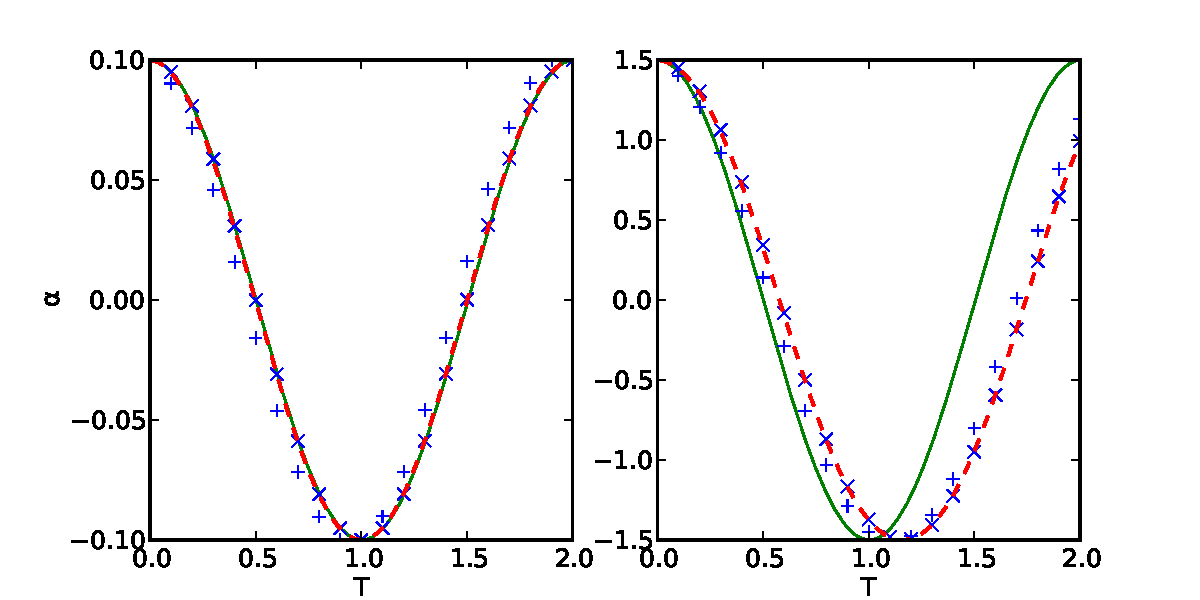
\includegraphics[width=\textwidth]{plots/pendel_loesung}
  \caption{Lösungen für ein Fadenpendel der Länge $l=1m$. Im linken Graphen
    ist die Ausgangslage $\alpha=1,5$, im rechten $\alpha=0,1$; in
    beiden Fällen ist die Ausgangsgeschwindigkeit 0. Die durchgezogene
  grüne Linie markiert die analytische Näherungslösung
  \eqref{eq:naeherung} für kleine Winkel. $\times$ markiert die
  Ergebnisse einer Integration mit dem einfachen Vorwärtsschritt
  \eqref{eq:simple} mit Zeitschritt $0,1s$, die gestrichelte rote
  Linie mit Zeitschritt $0,01s$. $+$ markiert die Lösung mit Hilfe des
  Velocity-Verlet-Algorithmus und Zeitschritt $0,1s$.}
  \label{fig:loesung}
\end{figure}

Für kleine Winkel gilt $\sin(\alpha)\approx\alpha$, und damit
\begin{equation}
  \ddot\alpha \approx = -\frac{g}{l}\alpha.
\end{equation}
Diese Differentialgleichung hat die allgemeine Lösung
\begin{equation}
  \alpha(t) = A \sin(\omega t + \phi)
  \label{eq:naeherung}
\end{equation}
mit $\omega=\sqrt{g/l}$, wie man sich leicht durch Einsetzen
überzeugt. Die Größen $A$ und $\phi$ ergeben sich aus den
Anfangsbedingungen, nämlich der Anfangsposition
\begin{equation}
  \alpha_0 = A \sin(\phi)
\end{equation}
und "~geschwindigkeit
\begin{equation}
  v_0 = A \omega \cos(\phi).
\end{equation}
Ist zum Beispiel $v_0=0$, so ist $\phi=\pi/2$ und $A=\alpha_0$, im
allgemeinen Fall ist
\begin{equation}
\phi =
\arctan\left(\frac{\alpha_0\omega}{v_0}\right)\quad\text{und}\quad
A = \frac{\alpha_0}{\sin(\phi)}.
\end{equation}
Wir haben nun eine geschlossene Lösung für die Position des Pendels,
so lange die Ausgangslage nicht zu sehr ausgelenkt ist. Um diese
Lösung zu visualisieren, nutzt man heute üblicherweise den Computer,
siehe Graph~\ref{fig:loesung}.

\subsection{Numerische Lösung}

Was passiert nun, wenn das System stärker ausgelenkt ist? Mit sehr
viel mehr Aufwand lässt sich auch für diesen Fall eine analytische
Lösung finden, allerdings in Form einer Reihe, die nicht mehr so
einfach zu zeichnen ist. Eine Alternative ist, die
Differentialgleichung \eqref{eq:pendelgln} mit Hilfe des Computers zu
berechnen. Wir sagen, wir "`simulieren"' das Pendel. Dazu fixieren wir
ein Einheitensystem, zum Beispiel eine Sekunde als Zeiteinheit und
einen Meter als Längeneinheit. In diesem System ist also $l=1$,
$g\approx 9,81$ und $\omega\approx 3,13$, falls des Pendel einen Meter
lang ist.

Zunächst müssen wir das Problem aber für den Computer anpassen, der ja
nur mit (endlich vielen) gewöhnlichen Zahlen rechnen kann, wir müssen
das Problem \emph{diskretisieren}. Wir betrachten nur die Zeitpunkte
\begin{equation}
  t_n = n\delta t, n=1(1)N,
\end{equation}
wobei der Zeitschritt $\delta t$ frei wählbar ist. Je kleiner $\delta
t$, desto genauer können wir $\alpha(t)$ bestimmen, allerdings steigt
natürlich die Anzahl der Schritte, die nötig sind, um eine feste
Gesamtzeit zu erreichen. Unsere Lösung, die Funktion $\alpha(t)$ wird
also durch ihre Werte $\alpha(t_n)$ an den diskreten Zeitpunkten
dargestellt.

\begin{figure}
  \centering
  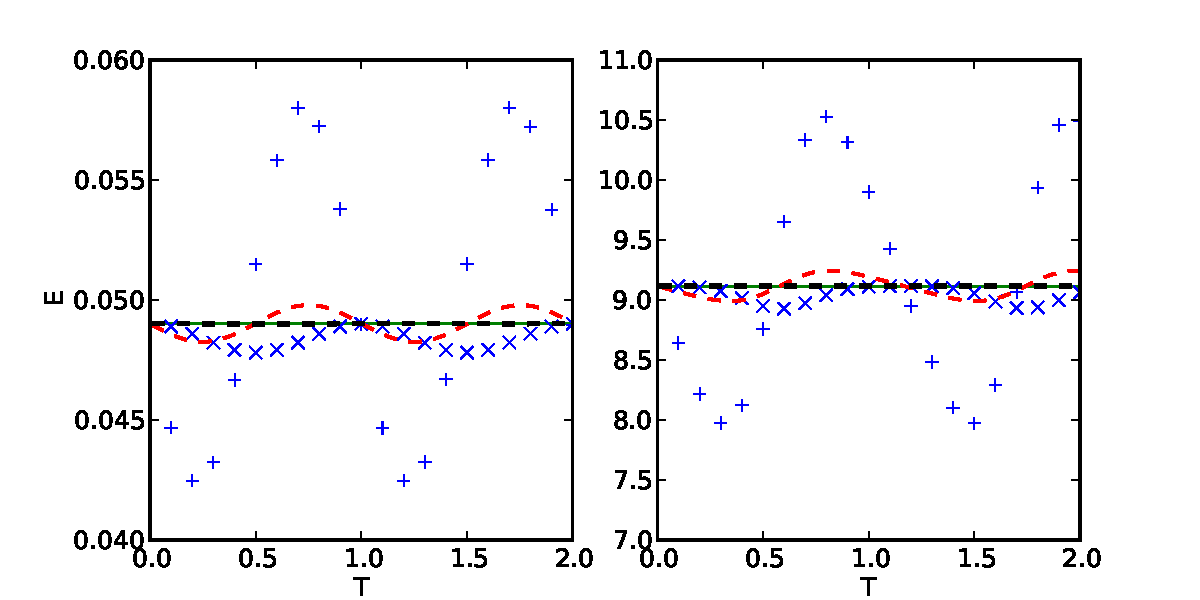
\includegraphics[width=\textwidth]{plots/pendel_energie}
  \caption{Energie als Funktion der Zeit, wieder für $l=1m$, und
    Ausgangslage $\alpha=1,5$ (links) und $\alpha=0,1$ (rechts) in
    Ruhe.  $+$ markiert die Ergebnisse einer Integration mit dem
    einfachen Vorwärtsschritt \eqref{eq:simple} mit Zeitschritt
    $0,1s$, die gestrichelte rote Linie mit Zeitschritt $0,01s$. $\times$
    markiert die Lösung mit Hilfe des Velocity-Verlet-Algorithmus und
    Zeitschritt $0,1s$, und die gestrichelte blaue Linie mit $0,01s$.}
  \label{fig:energie}
\end{figure}

Um Gleichung \eqref{eq:pendelgln} auf den Computer zu bringen, müssen
wir uns allerdings noch überlegen, wie wir mit der Ableitung verfahren.
Da wir die Ausgangsposition und "~ge\-schwin\-dig\-keit gegeben haben, liegt
es nahe, die Gleichung zu integrieren:
\begin{equation}
  v(t+\delta t) = \dot\alpha(t + \delta t) = v(t) + \int_{t}^{t+\delta t}
  -\omega^2\sin \alpha(\tau)\, d\tau.
\end{equation}
Da $\delta t$ aber unser Zeitschritt ist, wir also nichts weiter über
$\alpha(\tau)$ wissen, bietet sich die folgende Näherung an:
\begin{equation}
  v(t+\delta t) \approx v(t) - \omega^2\sin\alpha(t) \delta t.
\end{equation}
Analog ergibt sich dann durch nochmalige Integration:
\begin{equation}
  \alpha(t+\delta t) \approx \alpha(t) + v(t) \delta t.
  \label{eq:simple}
\end{equation}
Ausgehend von
\begin{equation}
  \alpha(0) = \alpha_0 \quad\text{und}\quad v(0) = v_0
\end{equation}
lässt sich damit also $\alpha(t)$ numerisch bestimmen. Der
Quellcode~\ref{lst:pendel} zeigt, wie eine einfach Implementation in
Python aussehen könnte.

Wie kann man nun überprüfen, ob diese Lösung tatsächlich korrekt ist?
Da das System abgeschlossen ist, muss seine Energie
\begin{equation}
  E = \frac{1}{2} l^2 v(t)^2 + gl (1 - \cos(\alpha(t)))
\end{equation}
erhalten sein. Lässt man sich diese allerdings ausgeben, stellt man
fest, dass $E(t)$ erheblich schwankt, vergleiche
Graph~\ref{fig:energie}. Dies lässt sich durch Verringern des
Zeitschritts beheben, das kostet aber entsprechend mehr Rechenzeit.

Eine bessere Alternative ist, den Algorithmus zu verbessern, was
wiederum etwas analytische Arbeit erfordert. Wir betrachten die
Taylorentwicklungen
\begin{align}
  \alpha\left(t+\delta t\right) &= \alpha\left(t+\frac{\delta t}{2}\right) + \frac{\delta t}{2}
  v\left(t+\frac{\delta t}{2}\right) + \frac{\delta t^2}{8} F\left(t+\frac{\delta t}{2}\right) + \O(\delta t^3)
  \intertext{und}
  \alpha\left(t\right) &= \alpha\left(t+\frac{\delta t}{2}\right) - \frac{\delta t}{2}
  v\left(t+\frac{\delta t}{2}\right) + \frac{\delta t^2}{8} F\left(t+\frac{\delta t}{2}\right) - \O(\delta t^3).
\end{align}
Durch Subtraktion ergibt sich
\begin{align}
  \alpha(t+\delta t) = \alpha(t) + \delta t\,v\left(t+\frac{\delta t}{2}\right) + \O(\delta t^4).
\end{align}
Die Geschwindigkeiten an den halben Zeitschritten erhält man einfach
durch $v(t + \delta t /2) = v(t) + \delta t F(t) / 2$.
Zusammengefasst ergibt sich der folgende \emph{Velocity-Verlet-Algorithmus}:
\begin{align}
  v\left(t + \frac{\delta t}{2}\right) &= v(t) + \frac{\delta t}{2} F(t) \\
  \alpha(t + \delta t) &= \alpha(t) + v\left(t + \frac{\delta t}{2}\right) \\
  v(t + \delta t) &= v\left(t + \frac{\delta t}{2}\right) + \frac{\delta t}{2}
  F(t + \delta t),
\end{align}
der anders als die direkte Vorgehensweise vorher numerisch stabil ist
und quasi keine Energieschwankungen aufzeigt, vergleiche
Graph~\ref{fig:energie}. 
Im Quellcode~\ref{lst:pendel} ist alternativ auch dieser Integrator
implementiert. Obwohl er nur unwesentlich komplizierter ist als der
einfache Integrator zuvor, erreicht etwa dieselbe Genauigkeit wie
dieser mit einem Zehntel der Zeitschritte.

Als weiterer Test bietet sich an, bei kleinen Auslenkungen mit der
analytisch bekannten Lösung zu vergleichen, die gut reproduziert wird,
siehe Graph~\ref{fig:loesung}. Bei größeren Anfangsauslenkungen oder
-ge\-schwin\-dig\-keiten ist die Abweichung allerdings sehr groß, weil
hier die analytische Näherung versagt. Im Rahmen ihrer Genauigkeit
erlaubt also die numerische Lösung, das vorgegebene Modell in einem
größeren Parameterraum auf sein Verhalten hin zu untersuchen, als
analytisch möglich wäre.

\lstinputlisting[style=floating,firstline=10,
caption={[Fadenpendel] Python-Code zum Fadenpendel
  mit graphisch aufbereiteter Ausgabe mit Hilfe der \texttt{matplotlib}.},
label=lst:pendel]{pendel.py}

%%% Local Variables: 
%%% mode: latex
%%% TeX-master: "padc"
%%% TeX-PDF-mode: t
%%% End: 

% Dies ist Teil der Vorlesung Physik auf dem Computer, SS 2012,
% Axel Arnold, Universitaet Stuttgart.
% 
% Dieses Werk ist unter einer Creative Commons-Lizenz vom Typ
% Namensnennung-Weitergabe unter gleichen Bedingungen 3.0 Deutschland
% zugänglich. Um eine Kopie dieser Lizenz einzusehen, konsultieren Sie
% http://creativecommons.org/licenses/by-sa/3.0/de/ oder wenden Sie sich
% schriftlich an Creative Commons, 444 Castro Street, Suite 900, Mountain
% View, California, 94041, USA.
\chapter{Lineare Algebra \textrm{I}}
\index{Gleichungssysteme>lineare}

Lineare Gleichungssysteme sind die einfachste Art von
Gleichungssystemen, für die sich zum Beispiel leicht bestimmen lässt,
ob und wieviele Lösungen es gibt. Daher führt man auch die Lösung
komplexerer Probleme, wie zum Beispiel Differentialgleichungen, oft
auf die Lösung eines Satzes von linearen Gleichungssystemen
zurück. Lineare Gleichungssysteme sind in diesem Sinne eine der
wesentlichen Grundlagen der numerischen Mathematik. Der händischen
Lösung der Systeme steht dabei vor allem ihre Größe im Weg ---
Finite-Elemente-Rechnungen können leicht die Lösung von
Gleichungssystemen mit Millionen von Variablen erfordern. Mit modernen
Algorithmen und Computern lassen sich solche Gleichungssysteme
allerdings schnell und zuverlässig lösen. In diesem Kapitel lernen wir
die grundlegende Methode zum Lösen von Gleichungssystemen kennen,
nämlich die allgemeine, aber langsame Gaußelimination. Daneben lernen
wir noch die LU-Zerlegung und die Choleskyzerlegung kennen, die mit
etwas Vorarbeit eine effizientere Lösung erlauben und im folgenden oft
zum Einsatz kommen werden.

Wir betrachten also folgendes Problem: Sei $A=(a_{ik})\in\RR^{m\times
  n}$, $b\in\RR^m$. Gesucht ist die Lösung $x\in\RR^n$ des
Gleichungssystems
\begin{equation}
  \label{eq:lgs}
  \begin{matrix}
    a_{11}x_1 &+&  a_{12}x_2 &+& \ldots &+& a_{1n}x_n &=& b_1\\
    a_{21}x_1 &+&  a_{22}x_2 &+& \ldots &+& a_{2n}x_n &=& b_2\\
    \vdots   &&   \vdots   &&         && \vdots  && \vdots\\
    a_{m1}x_1 &+&  a_{m2}x_2 &+& \ldots &+& a_{mn}x_n &=& b_m
  \end{matrix}
\end{equation}
oder kurz $Ax=b$. In dieser allgemeinen Form ist weder garantiert,
dass es eine Lösung gibt (z.B. $A=0$, $b\neq 0$), noch, dass diese
eindeutig ist ($A=0$, $b=0$).

\section{\keyword{Dreiecksmatrizen}}

Eine Matrix $A\in\RR^{n\times n}$ heißt eine \emph{rechte obere
  Dreiecksmatrix}, wenn sie quadratisch ist und $a_{ij}=0$ für $i>j$.
Analog kann man auch die linken unteren Dreiecksmatrizen definieren,
mit $a_{ij}=0$ für $i<j$. In jedem Fall bilden rechte obere und linke
untere Dreiecksmatrizen jeweils Unteralgebren der Matrixalgebra, d.h.,
sie sind abgeschlossen unter Addition und Multiplikation. Die
Schnittmenge dieser Algebren ist wiederum die Algebra der
\emph{\keyword{Diagonalmatrizen}}.

Ist $A$ eine rechte obere Dreiecksmatrix, so hat das Gleichungssystem
die Form
\begin{equation}
  \begin{matrix}
    a_{11}x_1 &+&  a_{12}x_2 &+& \ldots &+& a_{1n}x_n &=& b_1\\
             &&  a_{22}x_2 &+& \ldots &+& a_{2n}x_n &=& b_2\\
             &&            && \ddots && \vdots  && \vdots\\
             &&            &&        && a_{nn}x_n &=& b_n.
  \end{matrix}
\end{equation}
Dieses Gleichungssystem hat genau dann eine Lösung, wenn $A$ regulär
ist, also $\det A=\prod_{i=1}^na_{ii}\neq 0$. Die Lösung kann dann durch
\emph{Rücksubstitution} direkt bestimmt werden:
\begin{equation}
  \label{eq:ruecksubst}
  x_i = \frac{1}{a_{ii}}\left( b_i - \sum_{k=i+1}^n a_{ik}x_k\right)
  \quad\text{für}\; i=n(-1)1.
\end{equation}

Für reguläre \emph{linke untere Dreiecksmatrizen} ergibt sich die
Lösung entsprechend durch \emph{Vorwärtssubstitution}:
\begin{equation}
  \label{eq:vorwsubst}
  x_i = \frac{1}{a_{ii}}\left( b_i - \sum_{k=1}^{i-1} a_{ik}x_k\right)
  \quad\text{für}\; i=1(1)n.
\end{equation}

Für Diagonalmatrizen ist die Situation natürlich einfacher, es gilt
\begin{equation}
  x_i = \frac{1}{a_{ii}} b_i
  \quad\text{für}\; i=1(1)n.
\end{equation}

\begin{sloppypar}
  SciPy stellt für Dreiecksmatrizen spezielle Löserroutinen zur
  Verfügung, \scipy{scipy.linalg.solve_triangular(A, b, lower=False)},
  wobei \argd{lower} angibt, ob  \argd{A} eine linke untere statt rechte
  obere Dreiecksmatrix ist.
\end{sloppypar}

\section{\keyword{Gaußelimination}}

Die Gaußelimination ist ein Verfahren, um eine beliebiges
Gleichungssystem $Ax=b$, mit $A\in\RR^{m\times n}$, auf die
äquivalente Form
\begin{equation}
  \label{eq:rform}
  \begin{pmatrix}
    R & K \\
    0 & 0
  \end{pmatrix} x' = b'
\end{equation}
zu bringen, wobei $R$ eine reguläre rechte obere Dreiecksmatrix und
$K\in\RR^{k\times l}$ beliebig ist, und $x'$ eine Permutation
(Umordnung) von $x$. Dieses Gleichungssystem hat offenbar nur dann
eine Lösung, wenn $b_i'=0$ für $i=m-k+1(1)m$.

Diese ist im allgemeinen auch nicht eindeutig, vielmehr können die
freien Variablen $x_\text{K} = (x'_i)_{i=n-k+1}^{n}$ frei gewählt
werden. Ist $x_\text{R} = (x'_i)_{i=1}^{n-k}$ der Satz der
verbleibenden Lösungsvariablen, so gilt also
\begin{equation*}
  x_\text{L} = R^{-1}b' - R^{-1}K x_\text{K}.
\end{equation*}
Die Lösungen ergeben sich daraus als
\begin{equation}
  x' =
  \begin{pmatrix}
    R^{-1}b'\\
    0
  \end{pmatrix} +
  \left<
    \begin{pmatrix}
      -R^{-1}K_i\\
      e_i
    \end{pmatrix}
  \right>,
\end{equation}
wobei $K_i$ die $i$-te Spalte von K und
$\left<\right>$ den aufgespannten Vektorraum bezeichnet. Die
Ausdrücke, die $R^{-1}$ enthalten, können durch Rücksubstitution bestimmt
werden.

Um das System $Ax=b$, das wir im folgenden als $A|b$ zusammenfassen,
auf diese Form zu bringen, stehen folgende Elementaroperationen zur
Verfügung, die offensichtlich die Lösung nicht verändern:
\begin{enumerate}
\item Vertauschen zweier Gleichungen (Zeilentausch in $A|b$)
\item Vertauschen zweier Spalten in $x$ und $A$ (Variablenaustausch)
\item Addieren eines Vielfachen einer Zeile zu einer anderen
\item Multiplikation einer Zeile mit einer Konstanten ungleich 0
\end{enumerate}
Die Gausselimination nutzt nun diese Operationen, um die Matrix
spaltenweise auf die gewünschte Dreiecksform zu bringen. Dazu werden
Vielfache der ersten Zeile von allen anderen abgezogen, so dass die
Gleichung die Form
\begin{equation}
  \left(\begin{array}{lll|c}
      a_{11}^{(0)} & a_{12}^{(0)}\ldots &a_{1n}^{(0)} & b_1^{(0)}\\
      0     & a_{22}^{(1)}\ldots &a_{2n}^{(1)} & b_2^{(1)}\\
      \vdots& \vdots      &\vdots& \vdots\\
      0     & a_{m2}^{(1)}\ldots &a_{mn}^{(1)} & b_m^{(1)}\\
    \end{array}\right) =: A^{(1)} | b^{(1)}
\end{equation}
annimmt, wobei
\begin{equation}
  \begin{array}{rcll}
    a_{ik}^{(1)} &=& a_{ik}^{(0)} -  l_{i}^{(1)}a_{1k}^{(0)}
    & \quad\text{für}\; i=2(1)n, k=1(1)m\\[0.3em]
    b_{i}^{(1)} &=& b_{i}^{(0)} - l_{i}^{(1)} b_{1}^{(0)}
    & \quad\text{für}\; i=2(1)n \\[0.3em]
    a_{1k}^{(1)} &=& a_{1k}^{(0)},\quad b_{1}^{(1)} = b_{1}^{(0)}
    & \quad\text{sonst}
  \end{array}
  \quad\text{mit}\, l_{i}^{(1)} = \frac{a_{i1}^{(0)}}{a_{11}^{(0)}}.
\end{equation}
Mit dem verbleibenden Resttableau wird nun
genauso weiter verfahren:
\begin{equation}
  \label{eq:gausseli}
  \begin{array}{rcll}
    a_{ik}^{(r)} &=& a_{ik}^{(r-1)} -  l_{i}^{(r)}a_{r,k}^{(r-1)}
    & \quad\text{für}\; i=r+1(1)n, k=r(1)m\\[0.3em]
    b_{i}^{(r)} &=& b_{i}^{(r-1)} - l_{i}^{(r)} b_{r}^{(r-1)}
    & \quad\text{für}\; i=r+1(1)n \\[0.3em]
    a_{ik}^{(r)} &=& a_{ik}^{(r-1)},\quad b_{i}^{(r)} = b_{i}^{(r-1)}
    & \quad\text{sonst}
  \end{array}
  \text{mit}\, l_{i}^{(r)} = \frac{a_{ir}^{(r-1)}}{a_{rr}^{(r-1)}}.
\end{equation}
Das Verfahren ist beendet, wenn das Resttableau nur noch eine Zeile hat.

Ist während eines Schrittes $a_{rr}^{(r-1)} = 0$ und
\begin{enumerate}
\item nicht alle $a_{ir}^{(r-1)}=0$, $i=r+1(1)m$. Dann tauscht man
  Zeile $r$ gegen eine Zeile $i$ mit $a_{ir}^{(r-1)}\neq 0$, und fährt
  fort.
\item alle $a_{ir}^{(r-1)}=0$, $i=r(1)m$, aber es gibt ein
  $a_{ik}^{(r-1)}\neq 0$ mit $i,k\ge r$. Dann vertauscht man zunächst
  Zeile $r$ mit Zeile $i$, tauscht anschließend Spalte $k$ mit
  Spalte $r$, und fährt fort.
\item alle $a_{ik}^{(r-1)}=0$ für $i,k \ge r$. Dann hat
  $A^{(r-1)}|b^{(r-1)}$ die gewünschte Form \eqref{eq:rform} erreicht,
  und das Verfahren terminiert.
\end{enumerate}

Das Element $a_{rr}^{(r-1)}$ heißt auch \emph{Pivotelement}, da es
sozusagen der Dreh- und Angelpunkt des iterativen Verfahrens ist.  In
der Praxis ist es numerisch günstiger, wenn dieses Element möglichst
groß ist. Das lässt sich erreichen, in dem wie in den singulären
Fällen verfahren wird, also Zeilen oder Spalten getauscht werden, um
das betragsmäßig maximale $a_{ik}^{(r-1)}$ nach vorne zu
bringen. Folgende Verfahren werden unterschieden
\begin{itemize}
\item \emph{kanonische \keyword{Pivotwahl}}: es wird stets
  $a_{rr}^{(r-1)}$ gewählt und abgebrochen, falls dieses betragsmäßig
  zu klein wird. Diese Verfahren scheitert schon bei einfachen
  Matrizen (z.B. {\tiny $\begin{pmatrix} 0 & 1\\ 1 &
      0\end{pmatrix}$}), und kann daher nur eingesetzt werden, wenn
  die Struktur der Matrix sicherstellt, das $a_{rr}^{(r-1)}$ stets
  hinreichend groß ist.
\item \emph{Spaltenpivotwahl}: es wird wie oben im 1. Fall nur in der
  Spalte maximiert, d.h. wir wählen als  Pivotelement
  \begin{equation}
    i_0 = \text{argmax}_{i>r} \lvert a_{ir}^{(r-1)}\rvert
  \end{equation}
  und tauschen Zeilen $i_0$ und $r$; die Variablenreihenfolge bleibt
  unverändert. Ist die Matrix $A$ quadratisch, bricht das Verfahren
  genau dann ab, wenn $A$ singulär ist.
\item \emph{Totalpivotwahl}: wie oben im 2. Fall wird stets das maximale
  Matrixelement im gesamten Resttableau gensucht, also
  \begin{equation}
    i_0,k_0 = \text{argmax}_{i,k>r} \lvert a_{ik}^{(r-1)}\rvert.
  \end{equation}
  Dann vertauscht man zunächst Zeile $r$ mit Zeile $i_0$, und tauscht
  anschließend Spalte $k_0$ mit Spalte $r$, wobei man sich noch die
  Permutation der Variablen geeignet merken muss, zum Beispiel als
  Vektor von Indizes.
\end{itemize}

Unabhängig von der Pivotwahl benötigt die Gaußelimination bei
quadratischen Matrizen im wesentlichen $\O(n^3)$
Fließkommaoperationen. Das ist relativ langsam, daher werden wir
später bessere approximative Verfahren kennenlernen. Für Matrizen
bestimmter Struktur, zum Beispiel Bandmatrizen, ist die
Gaußelimination aber gut geeignet. NumPy bzw. SciPy stellen daher auch
keine Gaußelimination direkt zur Verfügung.
\scipy{scipy.linalg.solve(A, b)} ist ein Löser für Gleichungssysteme
$Ax=b$, der immerhin auf der LU-Zerlegung durch Gaußelimination
basiert. Dieser Löser setzt allerdings voraus, dass die Matrix nicht
singulär ist, also eindeutig lösbar.
 
\section{\keyword{Matrixinversion}}

Ist $A\in\RR^{n\times n}$ regulär, so liefert die Rücksubstitution
implizit die Inverse von $A$, da für beliebige $b$ das
Gleichungssystem $Ax=b$ gelöst werden kann. Allerdings muss das für
jedes $b$ von neuem geschehen. Alternativ kann mit Hilfe der
Gaußelimination auch die Inverse von $A$ bestimmt werden. Dazu wird
das Tableau $A|I$ in das Tableau $I|A^{-1}$ transformiert, wobei $I$
die $n\times n$-Einheitsmatrix bezeichnet. Die Vorgehensweise
entspricht zunächst der Gaußelimination mit
Spaltenpivotwahl. Allerdings werden nicht nur die Elemente unterhalb
der Diagonalen, sondern auch oberhalb eliminiert. Zusätzlich wird die
Pivotzeile noch mit $1/a_{ii}^{(i-1)}$ multipliziert, so dass das $A$
schrittweise die Form
\begin{equation}
  \left(\begin{array}{cccc}
      1     & 0      & a_{12}^{(2)}\ldots &a_{1n}^{(2)} \\
      0     & 1      & a_{22}^{(2)}\ldots &a_{2n}^{(2)} \\
      \vdots& 0      & a_{32}^{(2)}\ldots &a_{3n}^{(2)} \\
      \vdots& \vdots & \vdots             & \vdots      \\
      0     & 0      & a_{n2}^{(2)}\ldots &a_{nn}^{(2)} \\
    \end{array}\right)
\end{equation}
annimmt. Das Verfahren ist allerdings numerisch nicht sehr stabil, und
generell sollte die explizite Berechnung der Inversen wann inner
möglich vermieden werden. SciPy stellt die Matrixinversion als
Funktion \scipy{scipy.linalg.inv(A)} zur Verfügung.

Eine Ausnahme bilden Matrizen der Form $I + A$ mit $\lVert A \rVert =
\max \lVert Ax\rVert / \lVert x \rVert < 1$. Dann ist
\begin{equation}
  (I+A)^{-1} = I - A + A^2 - A^3 + \cdots
\end{equation}
eine gut konvergierende Näherung der Inversen.

\section{\keyword{LU-Zerlegung}}
\index{LR-Zerlegung}

Eine weitere Anwendung der Gaußelimination ist die LU-Zerlegung von
bestimmten quadratischen Matrizen. Dabei wird eine Matrix
$A\in\RR^{n\times n}$ so in eine ein linke untere Dreiecksmatrix $L$
und eine rechte obere Dreiecksmatrix $U$ zerlegt, dass $A=L\cdot U$.
Um die LU-Zerlegung eindeutig zu machen, vereinbart man üblicherweise,
dass $l_{ii}=1$ für $i=1(1)n$. Das $U$ steht übrigens für das
englische "`upper right"' und $L$ für "`lower left"'. Im Deutschen
findet sich vereinzelt noch der Begriff LR-Zerlegung, wobei hier L für
eine linke untere und R für eine rechte obere Matrix steht.

Ist eine solche Zerlegung einmal gefunden, lässt sich das
Gleichungssystem $Ax=b$ für beliebige $b$ effizient durch Vorwärts-
und Rücksubstitution lösen:
\begin{equation}
  L y = b,\, U x = y \quad\implies\quad Ax = L\,U x = L y = b.
\end{equation}
Zunächst wird also $y$ durch Vorwärtssubstitution berechnet,
anschließend $x$ durch Rückwärtssubstitution. Die Inverse lässt
sich so auch bestimmen:
\begin{equation}
  L y_i = e_i,\, U x_i = y_i\quad\text{für}\; i=1(1)n
  \quad\implies\quad  A^{-1} = \left(x_1,
    \ldots, x_n\right).
\end{equation}
Die Determinante von $A=L\cdot U$ ist ebenfalls einfach zu bestimmen:
\begin{equation}
  \det A = \det L\,\det U = \prod_{i=1}^n u_{ii}
\end{equation}

Um die LU-Zerlegung zu berechnen, nutzen wir wieder die
Gaußelimination.  Kann bei $A\in\RR^{n\times n}$ die Gaußelimination
in kanonischer Pivotwahl durchgeführt werden, so ist die LU-Zerlegung
von $A$ durch $U=A^{(n-1)}$, also die finale, auf rechte obere
Dreiecksform transformierte Matrix, und durch die Matrix
\begin{equation}
  L =
  \begin{pmatrix}
    1       &          &         &          & 0 \\
    l_1^{(0)} & 1       &         &           &  \\
    l_2^{(0)} & l_2^{(1)} & 1       &          &  \\
    \vdots  &          & \ddots & \ddots    & \\
    l_n^{(0)} & \ldots  & \ldots  & l_n^{(n-1)} & 1
  \end{pmatrix}
\end{equation}
der Updatekoeffizienten aus \eqref{eq:gausseli} gegeben.

Wie bereits gesagt, ist die Voraussetzung, dass die Gaußelimination
mit kanonischer Pivotwahl durchgeführt werden kann, stark, und
schließt selbst einfache Matrizen wie {\tiny $\begin{pmatrix} 0 & 1\\
    1 & 0\end{pmatrix}$} aus. Wie man sich leicht überlegt, besitzt
diese Matrix allerdings keine LU-Zerlegung.

Für manche Anwendungen ist es günstiger, wenn $L$ und $U$ normiert
sind. Dann benutzt man die \keyword{LDU-Zerlegung} $A=LDU$, mit $L$
linker unterer Dreiecksmatrix, $D$ Diagonalmatrix und $U$ rechter
oberer Dreiecksmatrix. Jetzt müssen $l_{ii}=1$ und $r_{ii}=1$
sein. Die LDU-Zerlegung ergibt sich aus der LU-Zerlegung durch $d_{ii}
= u_{ii}$ und $u'_{ik}=u_{ik}/u_{ii}$.

In SciPy ist die LU-Zerlegung in den Funktionen
\scipy{scipy.linalg.lu_factor(A)} oder \scipy{scipy.linalg.lu(A)} (zur
Zerlegung der Matrix A) und \scipy{scipy.linalg.lu_solve((lu,piv), b)}
(zum Lösen des LGS) implementiert.

\section{Cholesky-Zerlegung}
\index{Cholesky>-Zerlegung}

Wir betrachten im folgenden nur symmetrische, positiv definite
Matrizen, wie sie gerade in der Physik oft vorkommen. Auch in der
Optimierung spielen diese eine wichtige Rolle. Sei $A=LDU$ eine
LDU-Zerlegung einer symmetrischen Matrix, dann gilt
\begin{equation}
  LDU = A = A^T = (LDU)^T = U^T D L^T.
\end{equation}
Da die LDU-Zerlegung aber eindeutig ist und $U^T$ eine normierte,
linke untere Dreiecksmatrix und $L^T$ eine normierte, rechte obere
Dreiecksmatrix, so gilt $U=U^T$, und damit
\begin{equation}
  A = U^TDU = \widehat{U}^T\widehat{U} \quad\text{mit}\; \widehat{U}=\text{diag}(\sqrt{d_{ii}})U.
\end{equation}
Dies ist die Cholesky-Zerlegung. Anstatt die Gaußelimination
durchzuführen, lässt sich die Zerlegung aber auch direkt mit Hilfe des
\emph{Cholesky-Verfahrens}\index{Cholesky>-Verfahren} bestimmen: Sei
$A=\widehat{R}^T\widehat{R}$ eine Cholesky-Zerlegung.
Da $\widehat{R}$ unterhalb der Diagonalen nur 0 enthält, gilt
\begin{equation}
  a_{ik} = \sum_{l=1}^{i} \hat{r}_{li}\hat{r}_{lk} \quad\text{für}\;
  i=1(1)n,\,k=1(1)n.
\end{equation}
Daraus lässt sich die erste Zeile von $\widehat{R}$ direkt ablesen:
\begin{equation}
\hat{r}_{11} = \sqrt{a_{11}}\quad\text{und}\;
\hat{r}_{1k} = \frac{a_{1k}}{\hat{r}_{11}} \quad\text{für}\;k=2(1)n.
\end{equation}
Die nächsten Zeilen lassen sich analog bestimmen, da für jedes $i$
\begin{equation}
  a_{ii} = \sum_{l=1}^{i} \hat{r}_{li}^2\quad\implies\;
  \hat{r}_{ii} = \sqrt{a_{ii} - \sum_{l=1}^{i-1} \hat{r}_{li}^2}.
\end{equation}
Für die restlichen Elemente der Zeile gilt
\begin{equation}
  \hat{r}_{ik} = \frac{1}{\hat{r}_{ii}}\left(a_{ik} - \sum_{l=1}^{i-1}\hat{r}_{li}\hat{r}_{lk}\right) \quad\text{für}\;k=i+1(1)n
\end{equation}
Das Cholesky-Verfahren ist wie die Gaußelimination von der Ordnung
$\O(n^3)$, braucht aber nur halb so viele Operationen. In SciPy ist die
Cholesky-Zerlegung als \scipy{scipy.linalg.cholesky(A)} implementiert.

\section{\keyword{Bandmatrizen}}

Im folgenden werden wir oft mit $k$-Bandmatrizen zu tun haben, also
Matrizen, bei denen nur die Diagonale und einige Nebendiagonalen
besetzt sind. Diagonalmatrizen sind also 1-Bandmatrizen, eine
\emph{Dreibandmatrix}\index{Dreibandmatrizen} hat die Form
\begin{equation}
  \begin{pmatrix}
    d_1 & t_1    &     & & 0 \\
    b_1 & d_2    & t_2 \\
    {}  & \ddots & \ddots & \ddots \\
    {}  &        & b_{n-2} & d_{n-1} & t_{n-1}\\
    0   &        &        & b_{n-1} & d_n
  \end{pmatrix}.
\end{equation}
Für Matrizen dieser Form ist die Gaußelimination mit kanonischer
Pivotwahl sehr effizient, da pro Iteration jeweils nur die erste Zeile
des Resttableaus verändert werden muss. Dadurch ist der Rechenaufwand
nur noch linear in der Matrixgröße bzw. Länge der Bänder. Die
Dreiecksmatrizen $L$ und $U$ der LU-Zerlegung sind zusätzlich
(Drei-) Bandmatrizen, wobei $L$ nur auf der Haupt und der unteren
Nebendiagonalen von Null verschiedene Einträge hat, $U$ nur auf der
Diagonalen und der Nebendiagonalen oberhalb.

SciPy stellt für Bandmatrizen ebenfalls spezielle Löserroutinen zur
Verfügung, \scipy{scipy.linalg.solve_banded((l,u), A, b)},
wobei \argd{l} und \argd{u} die Anzahl der Nebendiagonalen oberhalb
und unterhalb angeben, und \argd{A} die Matrix in Bandform
angibt.

%%% Local Variables: 
%%% mode: latex
%%% TeX-master: "padc"
%%% TeX-PDF-mode: t
%%% End: 

% Dies ist Teil der Vorlesung Physik auf dem Computer, SS 2012,
% Axel Arnold, Universitaet Stuttgart.
% 
% Dieses Werk ist unter einer Creative Commons-Lizenz vom Typ
% Namensnennung-Weitergabe unter gleichen Bedingungen 3.0 Deutschland
% zugänglich. Um eine Kopie dieser Lizenz einzusehen, konsultieren Sie
% http://creativecommons.org/licenses/by-sa/3.0/de/ oder wenden Sie sich
% schriftlich an Creative Commons, 444 Castro Street, Suite 900, Mountain
% View, California, 94041, USA.

\chapter{Darstellung von Funktionen}

Auch moderne Prozessoren beherrschen nur die Grundrechenarten. Wie
kann man also auf einem Computer kompliziertere Funktionen berechnen,
wie z.B. die Sinusfunktion?

Beispielsweise könnte man die Funktionen als Vektor von
Funktionswerten speichern. Für die graphische Darstellung reicht das
aus, aber um Funktionen mit wenigstens sechs Stellen Genauigkeit im
Computer bereitzustellen, wären Millionen von Stützstellen nötig.

Daher müssen bessere Darstellungen für Funktionen genutzt werden.  Um
beliebige Funktionen auf dem Computer berechnen zu können, führt man
diese meist auf (stückweise definierte) Polynome zurück, die nur mit
Hilfe der Grundrechenarten berechnet werden können. Dies ist selbst
dann der Fall, wenn ein Prozessor gewisse Funktionen scheinbar in
Hardware implementiert hat; tatsächlich führt dieser intern die
notwendigen elementaren Operationen durch.

\section{\keyword{Horner-Schema}}
\label{sec:horner}

Die naive Auswertung eines Polynoms $\sum_{i=0}^{n} c_ix^{i}$ mit
$n+1$ Termen bzw.\ vom Grad $n$ benötigt $n$ Additionen und $2n$
Multiplikationen sowie einen Zwischenspeicher für die Potenzen $x^i$
des Arguments $x$. Besser ist die Auswertung des Polynoms nach dem
Horner-Schema:
\begin{equation}
  \label{eq:horner}
  \sum_{i=0}^{n} c_ix^{i} = c_0 + x(c_1 + x(c_2 + x(\ldots (c_{n-1} + x c_{n})))).
\end{equation}
Wird dieser Ausdruck von rechts nach links ausgewertet, so muss das
Ergebnis in jedem Schritt nur mit $x$ multipliziert und der nächste
Koeffizient addiert werden, was nur $n$ Multiplikationen und
Additionen benötigt. Auch muss kein Zwischenwert gespeichert werden,
was Prozessorregister spart. Als C-Code sieht die Auswertung des
Hornerschemas so aus:
\begin{lstlisting}[language=C]
double horner(double *series, int n, double x)
{
    double r = series[n];
    for(int i = n-1; i >= 0; --i)
        r = r*x + series[i];
    return r;
}
\end{lstlisting}
\sloppypar Die Polynomauswertung stellt NumPy als
\scipy{numpy.polyval(x, c)} zur Verfügung. \argd{c} bezeichnet die
Koeffizienten des Polynoms und \argd{x} das Argument, für das das
Polynom ausgewertet werden soll.

Eine weitere Anwendung des Hornerschemas ist die Polynomdivision durch
lineare Polynome der Form $x-x_0$, die zum Beispiel wichtig für die
iterative Bestimmung von Nullstellen ist. Es gilt nämlich
\begin{equation}
  \label{eq:polynomdiv}
  P(x) = \sum_{i=0}^{n} c_ix^{i} = 
  \left(\sum_{i=0}^{n-1} d_{i+1}x^{i}\right)(x-x_0) + d_0,
\end{equation}
wobei $d_i = c_i + x_0(c_{i+1} + x_0(\ldots (c_{n-1} + x_o c_n)))$ die
Zwischenterme des Hornerschemas bei Auswertung an der Stelle $x_0$
sind. $d_0$ ist dabei der Divisionsrest; ist $P(x)$ durch $x-x_0$
teilbar, so ist $d_0=0$. 

Dies zeigt man durch Induktion: für $P(x) = c_1 x + c_0$ ist offenbar
$P(x) = c_1(x-x_0) + c_0 + x c_1 = d_1(x-x_0) + d_0$. Für Grad $n$ ist
also
\begin{equation}
    P(x) = x \left(\sum_{i=0}^{n-1} c_{i+1}x^{i}\right) + c_0
    = x\left(\sum_{i=0}^{n-2} d'_{i+1}x^{i}(x-x_0) + d'_0\right) +
    d_0
\end{equation}
wobei sich die $d'_i = c_{i+1} + x_0(c_{i+2} + x_0(\ldots (c_{n-1} +
x_o c_n))) = d_{i+1}$ bei der Polynomdivision von $\sum_{i=0}^{n-1}
c_{i+1}x^{i}$ durch $x-x_0$ ergeben. Daher ist
\begin{equation}
    P(x) = \left(\sum_{i=0}^{n-2} d_{i+2}x^{i+1} + d_1\right)(x-x_0) +
    d_0 + x_0 d_1,
\end{equation}
was zu zeigen war.

\section{Taylorreihen}
\index{Taylorreihe}

\begin{figure}
  \centering
  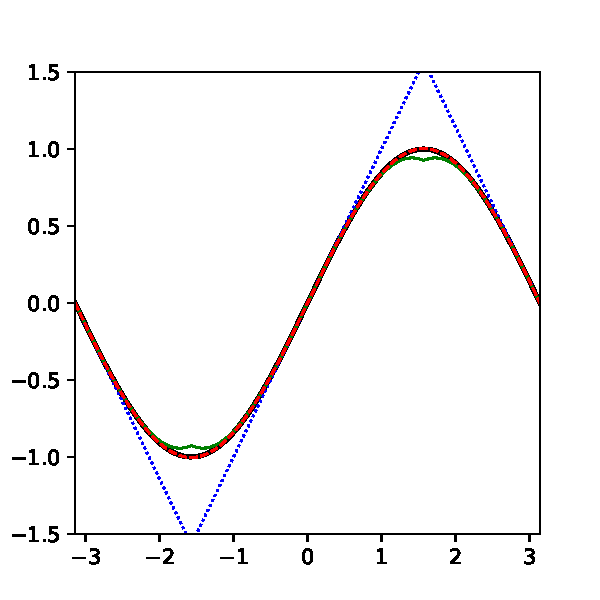
\includegraphics[width=0.5\textwidth]{plots/sinus}
  \caption{Näherung der Sinusfunktion durch die abgeschnittene
    Taylorreihe. Als schwarze durchgezogene Linie ist die tatsächliche
    Sinusfunktion dargestellt, blau gepunktet ist die Näherung erster
    Ordnung um Null, $x$, grün durchgezogen ist die kubische Näherung
    $x - x^3/6$, und rot gestrichelt $x-x^3/6 + x^5/120$. Die Kurven
    nutzen die Symmetrie der Sinuskurve, sind also an $\pm\pi/2$
    gespiegelt.}
  \label{fig:sinus}
\end{figure}

Nachdem wir nun wissen, wie Polynome effizient ausgewertet werden
können, stellt sich die Frage, wie man ein gutes Näherungspolynom für
eine Funktion bekommt. Dazu gibt es viele verschiedene Ansätze, deren
Vor- und Nachteile im Folgenden kurz besprochen werden. Der älteste
Ansatz, der auch in der Analytik weiten Einsatz findet, ist die
Taylorentwicklung.  Ist eine Funktion $f$ um einen Punkt $x_o$
hinreichend gut differenzierbar, lässt sie sich als bekannterweise
lokal als Taylorreihe darstellen:
\begin{equation}
  f(x) = \sum_{i=0}^\infty \frac{f^{(i)}(x_0)}{i!} (x-x_0)^i,
  \label{eq:taylor}
\end{equation}
wobei $f^{(i)}(x)$ die $i$-te Ableitung von $f$ an der Stelle $x$
bezeichnet.  Falls die Ableitungen existieren und $x-x_0$ klein genug
ist, so konvergiert diese Darstellung schnell, und einige Terme
genügen, um zufriedenstellende Genauigkeit zu erreichen. Lokal um den
Entwicklungspunkt $x_0$ is eine abgeschnittene Taylorreihe also eine
gute polynomielle Näherung. Leider gibt es für die meisten Funktionen
einen Konvergenzradius, außerhalb dessen die Reihe nicht einmal
konvergiert. Daher eignen sich Taylorreihen vor allem gut für kleine
Umgebungen. Auch ist eine abgeschnittene Taylorreihe nur im
Entwicklungspunkt $x_0$ exakt; dort stimmen allerdings gleich die
ersten $i$ Ableitungen.

Um  zum  Beispiel die  oben  angeführte  Sinusfunktion  mit 7  Stellen
Genauigkeit im Intervall $[0:\pi/2]$  auszuwerten, genügen die ersten 7
Terme der Taylorreihe. Mit Hilfe der Symmetrien der Funktion lässt sie
sich damit bereits für alle Argumente auswerten. Da
\begin{equation*}
  \sin'(x) = \cos(x) \quad\text{und} \quad \cos'(x) = -\sin(x),
\end{equation*}
ergibt sich die bekannte Reihe
\begin{equation}
  \sin(x) = \sum_{i=0}^\infty \frac{\sin^{(i)}(0)}{i!} x^i =
  \sum_{i=0}^\infty \frac{(-1)^i}{(2i+1)!} x^{2i+1}.
\end{equation}
Wie gut diese Darstellung mit entsprechender Rückfaltung funktioniert,
zeigt Abbildung~\ref{fig:sinus}.  Für viele andere komplexe Funktionen
ist es ebenfalls möglich, Taylorreihen analytisch oder numerisch zu
bestimmen, die dann zur Auswertung auf dem Computer genutzt werden
können.

\section{Polynom- oder Lagrangeinterpolation}
\index{Interpolation}
\index{Interpolation>Polynom-}
\index{Interpolation>Lagrange-}

\begin{figure}
  \centering
  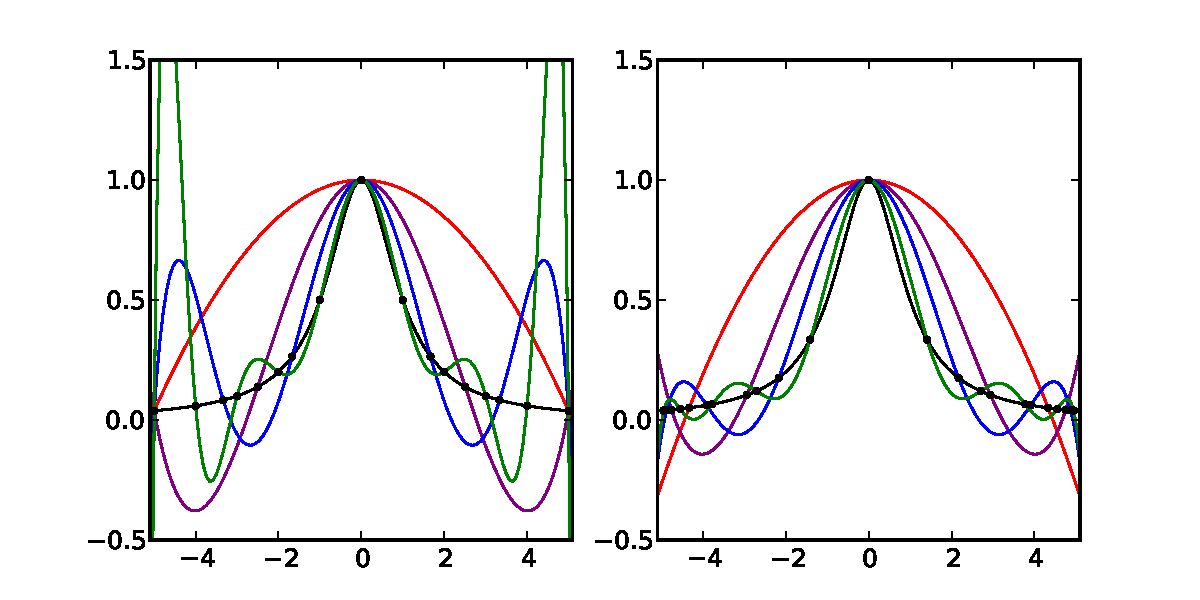
\includegraphics[width=\textwidth]{plots/runge_lagrange}
  \caption{Lagrange-Interpolation der Rungefunktion $1/(1+x^2)$
    (schwarze Linie). Im linken Graph sind die Stützstellen
    äquidistant gewählt (markierte Punkte), die farbigen Linien sind
    die interpolierenden Polynome durch 3 (rot), 5 (lila), 7 (blau)
    und 11 (grün) Stützstellen. Mit steigender Ordnung wird die
    Interpolation am Rand immer schlechter, das Polynom 10. Ordnung
    erreicht Werte bis nahe an zwei. Im rechten Graph sind
    für die gleichen Ordnungen Chebyshev-Stützstellen gewählt worden,
    die den Interpolationsfehler minimieren.}
  \label{fig:runge}
\end{figure}

Wie besprochen ist eine abgeschnittene Taylorreihe nur im
Entwicklungspunkt exakt (dann allerdings auch die Ableitungen),
innerhalb des Konvergenzradius nur eine Annäherung, und außerhalb des
Konvergenzradius sogar divergent.  Oft möchte man aber eher für einen
größeren Wertebereich eine gute (oder wenn möglich exakte) Darstellung
der Funktion haben.

Eine Möglichkeit dazu bietet die Polynom- oder
Lagrangeinterpolation. Dazu legt man eine Anzahl von Punkten im
gewünschten Wertebereich fest (die sogenannten \emph{Stützstellen}).
Wie sich zeigt, gibt es dann genau ein Polynom, dass die Funktion an
diesen Punkten exakt interpoliert. Genauer: seien Punkte $(x_i, y_i)$,
$i=0(1)n-1$ gegeben mit $x_i$ paarweise verschieden. Dann gibt es
genau ein Polynom $P(x)=\sum_{k=0}^{n-1} a_kx^{k}$ vom Grad $n-1$, so
dass $P(x_i) = y_i$, da die Gleichung
\begin{equation}
  \begin{split}
    y_1 &= P(x_0) = a_0 + a_1 x_0 + \cdots + a_{n-1}x_0^{n-1}\\
    \vdots\\
    y_n &= P(x_{n-1}) = a_0 + a_1 x_{n-1} + \cdots + a_{n-1}x_{n-1}^{n-1}
  \end{split}
  \label{eq:interpol}
\end{equation}
genau eine Lösung hat.

Leider ist aber nicht gewährleistet, dass mit steigender Anzahl von
Punkten die Funktion auch zwischen den Stützstellen immer besser
angenähert wird. Tatsächlich hat Runge ein einfaches Beispiel
angegeben, nämlich die Rungefunktion $1/(1+x^2)$, für die die Näherung
mit steigender Anzahl an äquidistanten Punkten immer schlechter wird,
siehe Abbildung~\ref{fig:runge}.

Bei der etwas allgemeineren Hermite-Interpolation können an den
Stützstellen neben den Funktionswerten auch Ableitungen vorgegeben
werden. Das eindeutige interpolierende Polynom hat dann einen Grad,
der der Gesamtanzahl an vorgegebenen Funktionswerten und Ableitungen
entspricht. Ist zum Beispiel nur eine Stützstelle $x_0$ gegeben und
neben dem Funktionswert $n$ Ableitungen, so entspricht das
Hermite-Polynom genau den ersten $n+1$ Termen der Taylorreihe.

Das interpolierende Polynom kann nicht nur zur Interpolation verwendet
werden, also der Bestimmung an Punkten zwischen den Stützstellen,
sondern --- mit Vorsicht --- auch zur Extrapolation, also um Werte
außerhalb des Bereichs zu bestimmen. Da bei der Hermite-Interpolation
auch die Ableitungen insbesondere am Rand kontrolliert werden können,
ist diese hier tendenziell vorteilhafter. Extrapolation spielt eine
wichtige Rolle, wenn eine direkte Auswertung der Zielfunktion
numerisch zu teuer oder unmöglich wird. Bei Computersimulationen tritt
dies insbesondere in der Nähe von kritischen Punkten auf.

In SciPy liefert die Funktion \scipy{scipy.interpolate.lagrange(x, y)}
das interpolierende Polynom durch die Stützstellen (\argd{x[i]},
\argd{y[i]}).

\subsection{\keyword{Lagrangepolynome}}

Die Koeffizienten $a_i$ können im Prinzip als Lösung von
Gleichung~\eqref{eq:interpol} mit geeigneten Lösern für lineare
Gleichungssysteme gefunden werden, was im allgemeinen allerdings recht
langsam ist. Daher benutzt man besser eine direkte Darstellung mit
Hilfe der \emph{Lagrangepolynome}, die wie folgt definiert sind:
\begin{equation}
  \label{eq:lagrange}
  L_i(x) = \prod_{k\neq i} \frac{x-x_k}{x_i-x_k}.
\end{equation}
Die Polynominterpolation wird daher auch Lagrange-Interpolation
genannt.  Wie man leicht sieht, gilt $L_i(x_k) = \delta_{ik}$, so dass
das Polynom\index{interpolierendes Polynom>Lagrangedarstellung}
\begin{equation}
  P(x) = \sum_{i=1}^n y_i\,L_i(x)
\end{equation}
das eindeutige interpolierende Polynom durch $(x_i, y_i)$
ist.

\index{interpolierendes Polynom>baryzentrische Darstellung}
Diese Darstellung ist allerdings für praktische Zwecke nur sinnvoll,
wenn sich die Stützstellen $x_i$ nicht ändern, da die Bestimmung der
Lagrangepolynome $L_i(x)$ zeitaufwändig ist. Geeigneter ist die
\emph{baryzentrische Darstellung}
\begin{equation}
P(x) = \sum_{i=0}^{n-1} y_i\, \mu_i \; \Big/ \; \sum_{i=0}^{n-1}
\mu_i\quad\text{mit}\quad
\mu_i := \frac{1}{x-x_i}\prod_{k\neq i}\frac{1}{x_i-x_k},
\end{equation}
bei der lediglich der Quotient zweier rationaler Funktionen gebildet
werden muss. 

\subsection{\keyword{Neville-Aitken-Schema}}

Das rekursive Neville-Schema ist eine effiziente Möglichkeit, das
interpolierende Polynom auszuwerten ohne es tatsächlich zu
berechnen. Das ist nützlich, wenn nur wenige Auswertungen nötig sind,
wie zum Beispiel beim Romberg-Integrationsverfahren, bei dem zur
Schrittweite 0 extrapoliert wird.

Wir definieren $P_{i,k}$ als das interpolierende Polynom der Ordnung
$k-1$ durch die Stützstellen $x_j, j=i(1)i+k-1$.  Gesucht ist der Wert
$P(x)=P_{0,n}(x)$ des interpolierenden Polynoms an der Stelle $x$.
Dann ist
\begin{align}
  P_{i,1}(x)&=y_i \quad\text{für}\, i=0(1)n-1
  \intertext{und}
  \label{eq:divdiff}
  P_{i,k}(x)&= \frac{P_{i,k-1}(x)(x_{i+k-1} - x) + P_{i+1,k-1}(x)(x -
    x_i)}{x_{i+k-1} - x_i} \quad\text{für}\, k=2(1)n, i=0(1)n-k,
\end{align}
da ja an den inneren Stützstellen $x_l$, $l=i+1(1)i+k-2$,
$P_{i,k-1}(x_l)=P_{i+1,k-1}(x_l) = y_l$ gilt, und per Konstruktion
$P_{i,k}(x_i)=y_i$ und $P_{i,k}(x_{i+k-1})=y_{i+k-1}$. Durch
sukzessives Berechnen zunächst der $P_{i,2}(x)$, dann der
$P_{i,3}(x)$, usw.\ lässt sich das interpolierende Polynom bequem an
einer fixen Stelle auswerten. Als (Neville-)Schema sieht das so aus:
\begin{center}
  \begin{tikzpicture}[on grid=true, node distance=1.5em and 10em]
    \node (u01) {$y_0$};
    \node[below=of u01] (u11) {$y_1$};
    \node[below=of u11] (u21) {$y_2$};
    \node[below=of u21] (u31) {$y_3$};
    \node[below=of u31] (u41) {$\vdots$};
  
    \node[right=of u11] (u02) {$P_{0,2}(x)$};
    \node[below=of u02] (u12) {$P_{1,2}(x)$};
    \node[below=of u12] (u22) {$P_{2,2}(x)$};
    \node[below=of u22] (u32) {$\vdots$};
  
    \node[right=of u12] (u03) {$P_{0,3}(x)$};
    \node[below=of u03] (u13) {$P_{1,3}(x)$};
    \node[below=of u13] (u23) {$\vdots$};

    \node[right=of u13] (u04) {$P_{0,3}(x)$};
    \node[below=of u04] (u14) {$\vdots$};

    \draw[->] (u01) -- (u02);
    \draw[->] (u11) -- (u02);
    \draw[->] (u11) -- (u12);
    \draw[->] (u21) -- (u12);
    \draw[->] (u21) -- (u22);
    \draw[->] (u31) -- (u22);

    \draw[->] (u02) -- (u03);
    \draw[->] (u12) -- (u03);
    \draw[->] (u12) -- (u13);
    \draw[->] (u22) -- (u13);

    \draw[->] (u03) -- (u04);
    \draw[->] (u13) -- (u04);
  \end{tikzpicture}
\end{center}
wobei die Pfeilpaare dividierte Differenzen gemäß \eqref{eq:divdiff} bedeuten.

\subsection{Newtonsche Darstellung}
\index{interpolierendes Polynom>Newtonsche Darstellung}

Wir betrachten nun die Polynome $P_{0,k}$ des Nevilleschemas. Es gilt
offenbar
\begin{equation}
  P_{0,k}(x) - P_{0,k-1}(x) = \gamma_k(x-x_0)\cdots(x-x_{k-2}),
\end{equation}
da die beiden Polynome in den Stützstellen $x_0,\ldots,x_{k-2}$
übereinstimmen und die Differenz ein Polynom vom Grad $k-1$ ist, also
höchstens $k-1$ Nullstellen hat. Weiter ist $\gamma_k$ der führende
Koeffizient des Polynoms $P_{0,k}(t)$, da $P_{0,k-1}(t)$ ja einen
niedrigeren Grad hat. Daraus ergibt sich die folgende \emph{Newtonsche
  Darstellung} des interpolierenden Polynoms:
\begin{equation}
  \begin{split}
    P_{0,n}(x) &= y_0 + \sum_{k=2}^{n} P_{0,k}(x) - P_{0,k-1}(x)\\
    &= y_0 + \gamma_2(x-x_0) + \gamma_3(x-x_0)(x-x_1) + \cdots
    + \gamma_n(x-x_0)\cdots(x-x_{n-2})\\
    &= y_0 + (x-x_0)\biggl(\gamma_2 + (x-x_1)\Bigl(\gamma_3 + \cdots
    \bigl(\gamma_{n-1} + (x-x_{n-2})\gamma_n\bigr)\cdots\Bigr)\biggr).
  \end{split}
\end{equation}
Die letztere Umformung zeigt, dass sich die Newtonsche Darstellung
effizient mit einem leicht abgewandelten Hornerschema auswerten lässt:
\begin{lstlisting}
def horner(x0, x, gamma):
    r = 0
    for k in range(len(x)-1, -1, -1):
        r = r*(x0-x[k]) + gamma[k];
    return r
\end{lstlisting}

Die Koeffizienten $\gamma_i$, $i=2(1)n$ lassen sich dabei bequem mit
dem Nevilleschema bestimmen. $\gamma_k$ ist ja der höchste Koeffizient
von $P_{0,k}$ ist, der sich leicht aus \eqref{eq:divdiff} berechnen
lässt. Wenn $\gamma_{i,k}$ den führenden Koeffizienten des Polynoms
$P_{i,k}$ bezeichnet, so erhalten wir das Nevilleschema
\begin{align}
  \gamma_{i,1} &= y_i \quad\text{für}\, i=0(1)n-1\quad\text{und}\\
  \gamma_{i,k}&= \frac{\gamma_{i+1,k-1} - \gamma_{i,k-1}}{x_{i+k-1} -
    x_i}
  \quad\text{für}\, k=2(1)n, i=0(1)n-k.
\end{align}
Da letztlich nur die $\gamma_{0,k}$ interessant sind, also die obere
Diagonale des Nevilleschemas, benötigt man für die Berechnung nur
einen Vektor
\begin{equation}
  \gamma' = \left(\gamma_{0,1},\gamma_{0,2},\ldots,\gamma_{0,k-1},
    \gamma_{0,k},\gamma_{1,k},\ldots,\gamma_{n-k,k}\right),
\end{equation}
der wie folgt berechnet wird:
\begin{lstlisting}
def neville(x, y):
    n = len(x)
    gamma = y.copy()
    for k in range(1, n):
        for i in range(n-k-1, -1, -1):
            gamma[i+k] = (gamma[i+k] - gamma[i+k-1])/(x[i+k] - x[i])
    return gamma
\end{lstlisting}
Man beachte, dass die Schleife über $i$ herunterläuft, um benötigte
Werte nicht zu überschreiben.

\subsection{\keyword{Chebyshev-Stützstellen}}

Bis jetzt haben wir wenig zur Wahl der Stützstellen gesagt. Oft liegt
es auch nahe, äquidistante Stützstellen zu verwenden wie im
Fadenpendel-Beispiel. Man kann allerdings zeigen, dass die
Chebyshev-Stützstellen den Fehler der Polynominterpolation minimieren.
Diese sind definiert als die Nullstellen der Polynome (!)
\begin{equation}
  \label{eq:chebyshev}
  T_n(\cos\phi) = \cos(n\phi),
\end{equation}
die offensichtlich zwischen -1 und 1 liegen und daher geeignet
skaliert werden müssen für die Interpolation in einem allgemeinen
Intervall. Die Chebyshev-Polynome $T_n$, $n\ge 0$, bilden eine
orthogonale Basis der Funktionen über $[-1,1]$ bezüglich des mit
$1/\sqrt{1-x^2}$ gewichteten Skalarprodukts. Daher kann jede genügend
glatte Funktion auf $[-1:1]$ als eine Reihe
\begin{equation}
  f(x) = \sum_{n=0}^\infty a_n T_n(x)
\end{equation}
dargestellt werden, die sogenannte Chebyshev-Reihe (siehe auch z.B.
\textcite{abramowitz70a}).

 Explizit sind diese Nullstellen gegeben durch
\begin{equation}
  x_{k,n} = \cos\left(\frac{2k+1}{2n}\pi\right),\quad k=0(1)n-1.
\end{equation}
Wird die Rungefunktion mit Chebyshevstützstellen interpoliert, so
konvergiert das interpolierende Polynom, im Gegensatz zu äquidistanten
Stützstellen.

\section{Splines}
\index{Spline}
\index{Interpolation>Spline-}

Wie wir gesehen haben, kann unter ungünstigen Umständen die Güte der
Polynominterpolation mit steigender Anzahl an Stützstellen sinken, vor
allem, wenn diese äquidistant verteilt sind. Oft ist das aber nicht zu
vermeiden, zum Beispiel, wenn die Daten in einem Experiment regelmäßig
gemessen werden. Das Problem ist, das die Koeffizienten des Polynoms
global gelten, sich glatte Funktionen aber nur lokal wie ein Polynom
verhalten (Taylorentwicklung!). Daher ist es günstiger, statt der
gesamten Funktion nur kleine Abschnitte durch Polynome zu nähern.

Der einfachste Fall einer solchen Näherung ist die \emph{lineare
  Interpolation}\index{Interpolation>lineare}, bei der die
Stützstellen durch Geraden, also Polynome vom Grad 1, verbunden
werden. Sind die Stützstellen $(x_i, y_i)$, $i=1(1)n$ gegeben, so ist
der lineare interpolierende Spline
\begin{equation}
  P_1(x) = \frac{(x_{i+1} - x)y_i + (x - x_i)y_{i+1}}
  {x_{i+1}-x_i}
  \quad\text{für}\, x_i \le x < x_{i+1}.
\end{equation}

\begin{figure}
  \centering
  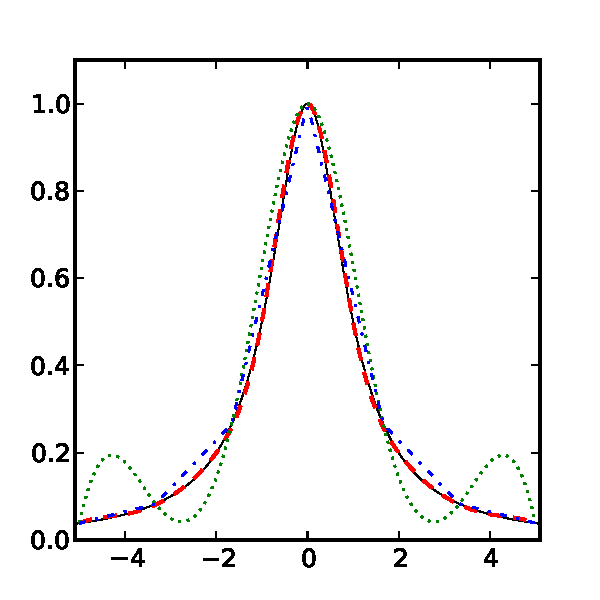
\includegraphics[width=0.5\textwidth]{plots/splines}
  \caption{Spline-Interpolation der Rungefunktion (durchgezogene
    schwarze Linie). Die gestrichelte blaue Linie ist die lineare
    Spline-Interpolierende mit 7 Stützstellen, die anderen Kurven sind
    kubische Splines mit 7 (grün gepunktet) und 11 Stützstellen (rot
    gestrichelt). Mit 11 Stützstellen ist der Spline von der
    Rungefunktion praktisch nicht mehr zu unterscheiden.}
  \label{fig:spline}
\end{figure}

Diese Funktionen sind aber an den Stützstellen im allgemeinen nicht
differenzierbar. Soll die Interpolierende differenzierbar sein, müssen
Polynome höherer Ordnung genutzt werden. Solche stückweise definierten
Polynome heißen \emph{Splines} --- das englische Wort Splines
bezeichnete dünne Latten, die vor dem Computerzeitalter benutzt
wurden, um glatte, gebogene Oberflächen vor allem für Schiffsrümpfe zu
entwickeln. Der wichtigste Spline ist der \emph{kubische} oder
\emph{natürliche}
Spline\index{Spline>kubisch}\index{Spline>natürlich}, der aus
Polynomen dritten Grades zusammengesetzt und zweifach stetig
differenzierbar ist. Seine allgemeine Form ist
\begin{equation}
  P_3(x) = y_i + m_i(x-x_i) + \frac{1}{2}M_i(x-x_i)^2 + \frac{1}{6}\alpha_i(x-x_i)^3
  \quad\text{für}\, x_i \le x < x_{i+1}.
\end{equation}
Da die zwei rechten und linken zweiten Ableitungen an den Stützstellen
übereinstimmen müssen, gilt
\begin{equation}
  \alpha_i = \frac{M_{i+1} - M_i}{x_{i+1} - x_i}.
\end{equation}
Aus der Gleichheit der Funktionswerte an den Stützstellen ergibt sich
\begin{equation}
  m_i = \frac{y_{i+1} - y_i}{x_{i+1}-x_i} -
  \frac{1}{6}(x_{i+1}-x_i)(2M_i + M_{i+1}).
\end{equation}
Aus der Gleichheit der ersten Ableitungen ergibt sich schließlich ein
Gleichungssystem für die $M_i$. Hier kommen in den Gleichungen
gleichzeitig $M_{i-1}$, $M_i$ und $M_{i+1}$ vor, daher müssen für die
Randwerte weitere Vorgaben gemacht werden. Sollen die Splines am Rand
festgelegte 2. Ableitungen $M_0$ und $M_n$ haben, so hat das
Gleichungssystem die Form
\begin{equation}
  \label{eq:spline1}
  \begin{pmatrix}
    2      & \lambda_1 &           &           &           &         0 \\
    \mu_2  & 2         & \lambda_2 \\
           &           & \ddots    & \ddots    & \ddots \\
           &           &           & \mu_{n-2}  & 2         & \lambda_{n-2} \\
    0      &           &           &           & \mu_{n-1}  & 2         \\
  \end{pmatrix}
  \begin{pmatrix}
    M_1\\
    M_2\\
    \vdots\\
    M_{n-2}\\
    M_{n-1}
  \end{pmatrix} \,=\,
  \begin{pmatrix}
    6S_1 - \mu_1 M_0\\
    6S_2\\
    \vdots\\
    6S_{n-2} \\
    6S_{n-1} -  \lambda_{n-1} M_n
  \end{pmatrix},
\end{equation}
mit
\begin{equation}
  \lambda_i = \frac{x_i - x_{i-1}}{x_{i+1} - x_{i-1}},\quad
  \mu_i = \frac{x_{i+1}-x_i}{x_{i+1} + x_{i-1}}\quad\text{und}\quad
  S_i = \frac{\frac{y_{i+1}-y_i}{x_{i+1} -
      x_i} - \frac{y_i-y_{i-1}}{x_i - x_{i-1}}}{x_{i+1}-x_{i-1}}.
\end{equation}
Auch periodische Funktionen können kubisch interpoliert werden, wobei
dann die zusätzliche Bedingungen durch die Kontinuität über die periodische
Grenze hinweg gegeben sind. Die Gleichungen für $\alpha_i$ und $m_i$
sind dabei unverändert, nur das Gleichungssystem wird
\begin{equation}
  \label{eq:spline2}
  \begin{pmatrix}
    2      & \lambda_1 &           &           &           &      \mu_1 \\
    \mu_2  & 2         & \lambda_2 &           & 0\\
           &           & \ddots    & \ddots    & \ddots \\
           & 0          &           & \mu_{n-2}  & 2         & \lambda_{n-2} \\
    \lambda_{n-1} &           &           &           & \mu_{n-1}  & 2         \\
  \end{pmatrix}
  \begin{pmatrix}
    M_1\\
    M_2\\
    \vdots\\
    M_{n-2}\\
    M_{n-1}
  \end{pmatrix} \,=\,
  \begin{pmatrix}
    6S_1\\
    6S_2\\
    \vdots\\
    6S_{n-2} \\
    6S_{n-1}
  \end{pmatrix},
\end{equation}
wobei die Funktion als $x_n-x_1$-periodisch mit $y_1=y_n$
vorausgesetzt wird. Abbildung~\ref{fig:spline} zeigt die
Spline-Interpolation der Rungefunktion, die für diesen
Interpolationstyp keine Probleme zeigt.

Die Gleichungssysteme \eqref{eq:spline1} und \eqref{eq:spline2} sind
sehr gut konditioniert und mit einem einfachen Gleichungslöser zu
behandeln.  Zum Beispiel ist die Gauß-Elimination ist für die hier
auftretenden einfachen Bandstrukturen sehr effizient. In SciPy gibt es
selbstverständlich bereits eine fertige Routine für die
Spline-Interpolation, nämlich \scipy{scipy.interpolate.interp1d(x, y,
  kind)}. (\argd{x},\argd{y}) sind dabei die Stützstellen, und
\argd{kind} eine Zeichenkette, die den Typ des Splines
bestimmt. Mögliche Werte sind zum Beispiel "`linear"' und "`cubic"'
für lineare bzw..\ kubische interpolierende Splines.

\section{Ausgleichsrechnung, Methode der kleinsten Quadrate}
\index{Ausgleichsrechnung}
\index{Fitting}
\index{Methode der kleinsten Quadrate}

\begin{figure}
  \centering
  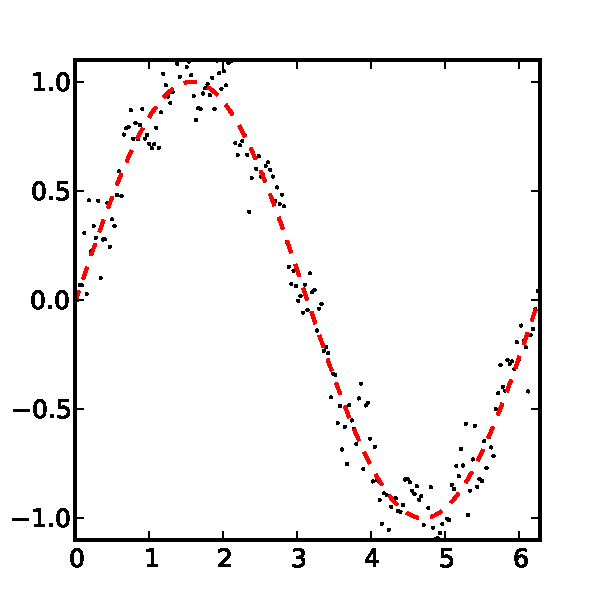
\includegraphics[width=0.5\textwidth]{plots/leastsq}
  \caption{Methode der kleinsten Quadrate zum Fitten der Sinusfunktion
    $y=\sin(x)$. 200 Datenpunkte zwischen 0 und $2\pi$ wurden als
    $\sin(x) + 0,1\,\sin(10 x) + \xi$ erzeugt, wobei $\xi$ eine
    Gauß-verteilte Pseudozufallsvariable mit Varianz $0,01$ war. Die
    resultierende Sinusfunktion (rot gestrichelt) hat die Form $a
    \sin(bx+c)$, wobei die Koeffizienten auf gut 2\% Genauigkeit
    $a=b=1$ und $c=0$ entsprechen. Die kleine höherfrequente
    Schwingung kann durch einen Fit allerdings nicht zuverlässig
    erkannt werden.}
  \label{fig:leastsq}
\end{figure}

Interpolierende Polynome, Taylorreihen und Splines haben gemeinsam,
das diese exakt durch die gegebenen Stützstellen verlaufen. Oftmals
ist das aber gar nicht gewünscht, da die Daten selbst nicht exakt
sind, zum Beispiel wenn diese aus einem Experiment oder einer
Simulation stammen. In diesem Fall hat man üblicherweise eine
Vorstellung, welche funktionelle Form die Daten annehmen, und möchte
nun wissen, mit welchen Parametern diese Funktion am besten mit den
Daten verträglich ist. Dazu muss man den Parametersatz bestimmen, so
dass der Abstand der Daten von der Funktion minimiert wird.

Seien also wieder Daten $(x_i, y_i)$, $i=1(1)n$ und eine Funktion
$f_v(x)$ gegeben. Gesucht ist dann derjenige Parametervektor $v$, der
die Abweichung
\begin{equation}
  \label{eq:leastsq}
  \Delta(v) = \sum_i (f_v(x_i) - y_i)^2
\end{equation}
minimiert. Dieses Verfahren wird auch Methode der kleinste Quadrate
genannt, da ja die quadrierten Abweichungen minimiert werden
sollen. Ist $f_{a,b}(x) = ax + b$ eine Gerade, spricht man auch von
\emph{linearer Regression}\index{lineare Regression}. In diesem Fall lässt
sich das Optimum einfach bestimmen, da
\begin{equation}
  0 = \frac{d}{da} \Delta(a,b) = \sum_i 2 (a x_i + b - y_i)x_i
  = 2N \left(a  \left<x_i^2\right> + b \left<x_i\right> -
    \left<y_ix_i\right> \right)
\end{equation}
und
\begin{equation}
  0 = \frac{d}{db} \Delta(a,b) = \sum_i 2 (a x_i + b - y_i)
  = 2N \left(a  \left<x_i\right> + b - \left<y_i\right> \right),
\end{equation}
wobei $\left<\cdot\right>$ den Mittelwert über alle Datenpunkte
bedeutet. Daraus ergibt sich
\begin{equation}
  a = \frac{\left<y_ix_i\right> -
    \left<y_i\right>\left<x_i\right>}{\left<x_i^2\right>-\left<x_i\right>^2}
  \quad\text{und}\;
  b = \left<y_i\right> - a \left<x_i\right>,
\end{equation}
was sich einfach auf dem Computer berechnen lässt.

Auch für quadratische und andere einfache Funktionen lassen sich die
Koeffizienten geschlossen darstellen, aber bei allgemeinen Funktionen
ist dies nicht immer der Fall. Dann muss die nichtlineare
Optimierungsaufgabe \eqref{eq:leastsq} numerisch gelöst werden, was
wir später behandeln werden. Für den Moment genügt uns, dass SciPy die
Funktion \scipy{scipy.optimize.leastsq(delta, v0, (x, y))} dafür
bereitstellt. \argd{(x, y)} sind dabei die Ausgangsdaten, die hier zu
einem Tupel zusammengefasst sind. \argd{v0} ist der Startwert für die
Berechnung, der nicht zu weit vom (unbekannten) Optimum entfernt
liegen darf. \argd{delta} ist eine Python-Funktion, die als Argumente
$v$, $x_i$ und $y_i$ nimmt und $f_v(x_i) - y_i$ zurückliefert.  Da
$f_v(x)$ eine beliebig komplizierte Form annehmen kann, ist diese
Aufgaben im allgemeinen nicht lösbar, allerdings funktioniert ein
solcher \emph{Fit} für einfache Funktionen meistens recht
gut. Abbildung~\ref{fig:leastsq} zeigt einen solchen Funktionsfit an
eine verrauschte Sinusfunktion, die mit 200 Datenpunkten auf etwa 2\%
genau gefittet werden kann. Man beachte, das der Ausgangswert für den
Fit mit Hilfe der SciPy-Funktion \lstinline!leastsq! $a=0$, $b=1$,
$c=0$ war; beim Startwert $a=0$, $b=0$, $c=0$ bricht das Verfahren
ab. Das zeigt, dass man tatsächlich nicht zu weit vom Optimum starten
kann, was ein gewisses Verständnis der Zielfunktion voraussetzt.

Ist die Funktionsform, die den Daten zugrundeliegt, unbekannt, ist es
normalerweise keine gute Idee, die Form zu raten. Generell sollte auch
die Anzahl der Parameter sehr klein sein, da sich sonst fast alles
"`gut"' fitten lässt ("`With four parameters I can fit an elephant and
with five I can make him wiggle his trunk."' --- J. von Neumann).

Soll aber zum Beispiel für Visualisierungszwecke eine ansprechende
Kurve entlang der Daten gelegt werden, deren tatsächliche Abhängigkeit
unbekannt ist, dann sind \emph{Pad\'e-Funktionen} oft eine gute
Wahl. Diese haben die Gestalt $P(x)/Q(x)$, wobei $P$ und $Q$ zwei
Polynome mit paarweise verschiedenen Nullstellen sind. Üblicherweise
lassen sich schon niedrigen Polynomgraden ansprechende Fits finden,
sofern die Grade der beiden Polynome in etwa gleich gewählt werden.

\section{Fourierreihen}

Bis jetzt waren unsere Näherungsfunktionen auf Polynomen basierend, da
diese einerseits vom Computer verarbeitet werden können und
andererseits aufgrund der Taylorentwicklung glatte Funktionen meist
gut approximieren. Für periodische Funktionen sind Polynome aber an
sich erst einmal wenig geeignet, da sie selbst nicht periodisch
sind. Splines können zwar auch periodisch gemacht werden, aber
trotzdem sind trigonometrische Funktionen besser geeignet, um
periodische Funktionen darzustellen. Fourierreihen und
-transformationen stellen Funktionen als trigonometrische Reihen dar,
die meist gut konvergieren und darüber hinaus einige nützliche
Eigenschaften haben.

Es gibt zwei Hauptanwendungen der Fourierdarstellung: die Analyse und
Aufbereitung periodischer Signale und die Lösung von
Differentialgleichungen.  Bei periodischen Signalen dient die
Fourierdarstellung zur Analyse des \emph{Spektrums} des Signals.
Diese gibt nützliche Informationen über die charakteristischen
Zeitskalen von Strukturen im Signal, zum Beispiel die Tonhöhe und die
Obertonreihe eines Instruments. In dieser Frequenzdarstellung lassen
sich auch gezielt einzelne Frequenzen dämpfen, was Rauschen
unterdrücken kann und im ursprünglichen Funktionsraum teure Faltungen
erfordert.  Bei Differentialgleichungen nutzt man aus, dass die
Ableitung im Frequenzraum eine algebraische Operation ist, und die
Differentialgleichung somit in eine gewöhnliche algebraische (und oft
sogar lineare) übergeht.

\subsection{Komplexe Fourierreihen}
\index{Fourierreihen>komplexe}
\index{Fouriertransformation>komplexe}
Wir betrachten eine periodische Funktion $f(t)$ mit $f(t+T) = f(t)$
für alle $t\in\RR$, d.h. $f$ hat Periode $T$. Dann ist die
Fourierdarstellung von $f$ gegeben durch
\begin{equation}
  \label{eq:fourier}
  f(t) = \sum_{n\in\ZZ} \hat{f}_n e^{i n\omega t}
\end{equation}
mit $\omega=2\pi/T$. Die Koeffizienten $\hat{f}_n$ lassen sich
berechnen als
\begin{equation*}
  \label{eq:fouriercoeff}
  \hat{f}_n = \frac{1}{T}\int_0^T f(t)e^{-i n\omega t}\, dt
\end{equation*}
und sind im allgemeinen komplex, auch wenn $f$ reellwertig ist. Die
Beiträge $\hat{f}_{\pm n}$ haben dieselbe Frequenz $\pm n/T$,
unterscheiden sich aber in ihrer Phase. Die \emph{Leistung} zu dieser
Frequenz ist $\hat{f}_{n}\hat{f}_{-n}$.

\eqref{eq:fourier} lässt sich auch so lesen, dass
\begin{equation}
  e^{-i n\omega t} = \cos(n \omega t) + i \sin(n \omega t)
\end{equation}
eine orthonormale Basis bezüglich des Skalarprodukts
\begin{equation}
  \label{eq:l2scalar}
  (f, g) = \frac{1}{T}\int_0^T f(t)\overline{g(t)}\,dt
\end{equation}
bilden. Ähnlich wie ein Vektor im $\RR^n$ wird die Funktion $f$ also
durch die Fouriertransformation in ihre Schwingungskomponenten
zerlegt.  Insbesondere sind die Fourierkoeffizienten linear in der
Funktion, d.h.
\begin{equation}
  \widehat{f+\lambda g}_n = \hat{f}_n +\lambda \hat{g}_n.
\end{equation}

Die Voraussetzungen für die Konvergenz der Fourierreihe sind sehr
schwach - solange die Funktion wenigstens quadratintegrabel ist,
konvergiert die Fourierreihe fast überall, d.h.
\begin{equation}
  \left\lVert f(t) - \sum_{n=-N}^N \hat{f}_n e^{i n\omega t} \right\rVert \xrightarrow{N\to\infty} 0.
\end{equation}
Daneben ist die Transformation $f\to\hat{f}$ eine \emph{Isometrie},
genauer gilt das \emph{\keyword{Parsevaltheorem}}
\begin{equation}
  \sum_{n\in\ZZ} \lvert\hat{f}_n\rvert^2 =
  \frac{1}{\omega}\int_0^t \lvert f(t)\rvert^2\,dt.
\end{equation}
Das Parsevaltheorem besagt auch, dass die Restbeiträge von großen $n$
immer kleiner werden, so dass also eine abgeschnittene Fourierreihe
eine Approximation an die gesuchte Funktion darstellt. Anders als
abgeschnittene Taylorreihen, die nur in einer schmalen Umgebung um den
Aufpunkt exakt sind, konvergiert die Fourierreihe
gleichmäßig. Allerdings muss die abgeschnittene Fourierreihe im
allgemeinen keinen einzigen Punkt mit der Zielfunktion gemeinsam
haben, anders als Taylorreihen oder Splines.

Weiter gilt:
\begin{itemize}
\item Die Fourierreihe über einem Intervall $[0,T)$ kann aus der
  Fourierreihe für das Intervall $[0,2\pi)$ durch Streckung mit
  $\omega$ berechnet werden:
  \begin{equation}
    \widehat{f(t)}_n = \frac{1}{T}\int_0^T f(t)e^{-i n\omega t}\, dt
    = \frac{1}{2\pi}\int_0^{2\pi} f(t'/\omega)e^{-i n t'}\, dt',
  \end{equation}
\item Es gilt
  \begin{equation}
    \widehat{f(t + t_0)}_{n} = e^{i n \omega t_0} \widehat{f(t)}_{n}
  \end{equation}
  die Phase kann also nach Belieben verschoben werden. Die Leistung
  $\hat{f}_{n}\hat{f}_{-n}$ bleibt dabei natürlich erhalten.
\item Für die komplexe Konjugation gilt stets
  $\widehat{\overline{f}}_n = \overline{\hat{f}_n}$, da die
  Fouriertransformation ja linear ist.
\item Ist Funktion $f$ symmetrisch, also $f(t) = f(-t) = f(T-t)$, so ist
  $\hat{f}_{-n} = \hat{f}_n$, also $\hat{f}$ symmetrisch.
\item Ist Funktion $f$ ungerade, also $f(t) = -f(-t) = -f(T-t)$, so ist
  $\hat{f}_{-n} = -\hat{f}_n$, also $\hat{f}$ ungerade.
\item Ist Funktion $f$ reellwertig, also $f(t) = \overline{f(t)}$, so
  ist $\hat{f}_{-n} = \overline{\hat{f}_n}$. Allerdings sind die
  Fourierkoeffizienten im allgemeinen komplex!
\item 
  Ist die komplexwertige Funktion $f(t)=g(t) + ih(t)$ mit $g$, $h$
  reellwertig, gilt also
  \begin{equation}
    \hat{f}_{n}  + \hat{\overline{f}}_{n} = \widehat{2g}_{n}
    \quad\text{und}\;
    \hat{f}_{n}  - \hat{\overline{f}}_{n} = \widehat{2ih}_{n}.
  \end{equation}
  Dies bedeutet, dass sich die Fourierreihen zweier reellwertiger
  Funktionen zusammen berechnen und anschließend wieder trennen
  lassen. Da die Berechnung der Fourierkoeffizienten sowieso komplex
  erfolgen muss, erspart dies bei numerischer Auswertung eine
  Transformation.
\item Die Ableitung der Fourierreihe ist sehr einfach:
  \begin{equation}
    \frac{d}{dt}  f(t) = \sum_{n\in\ZZ} \hat{f}_n i n\omega e^{i n\omega
      t} = \sum_{n\in\ZZ} \widehat{\left(\frac{df}{dt}\right)}_n e^{i n\omega
      t}\quad\implies\quad \widehat{\left(\frac{df}{dt}\right)}_n= i n\omega\hat{f}_n.
  \end{equation}
\end{itemize}

\subsection{Reelle Fourierreihen}
\index{Fourierreihen>reelle}
\index{Fouriertransformation>reelle}

Da die Fourieranalyse besonders zur Analyse und Bearbeitung von
Messdaten genutzt wird, sind die Fourierreihen reellwertiger
Funktionen besonders wichtig. Ist die Funktion $f$ rellwertig, so ist
\begin{multline}
  \hat{f}_{n}e^{in \omega t} + \hat{f}_{-n}e^{-in \omega t} =
  \hat{f}_{n}e^{in \omega t} + \overline{\hat{f}_{-n}e^{in \omega t}}
  = 2\Re(\hat{f}_{n}e^{in \omega t})\\
  = 2\Re(\hat{f}_{n})\cos(n \omega t) - 2\Im(\hat{f}_{n})\sin(n \omega t).
\end{multline}
Daraus folgt, dass sich die Fourierreihe auch komplett reellwertig
schreiben lässt:
\begin{equation}
  f(t) = \frac{a_0}{2} + \sum_{n=1}^\infty a_n \cos(n\omega t) + b_n
  \sin(n\omega t)
\end{equation}
mit
\begin{align}
  a_n &= 2\Re(\hat{f}_{n}) = \frac{2}{T}\int_0^T f(t)\cos(n\omega t)\,
  dt
  \intertext{und}
  b_n &= -2\Im(\hat{f}_n) = \frac{2}{T}\int_0^T f(t)\sin(n\omega t)\,
  dt.
\end{align}
Für symmetrische Funktionen ist offenbar $b_n=0$, für ungerade
Funktionen $a_n=0$.

\begin{figure}
  \centering
  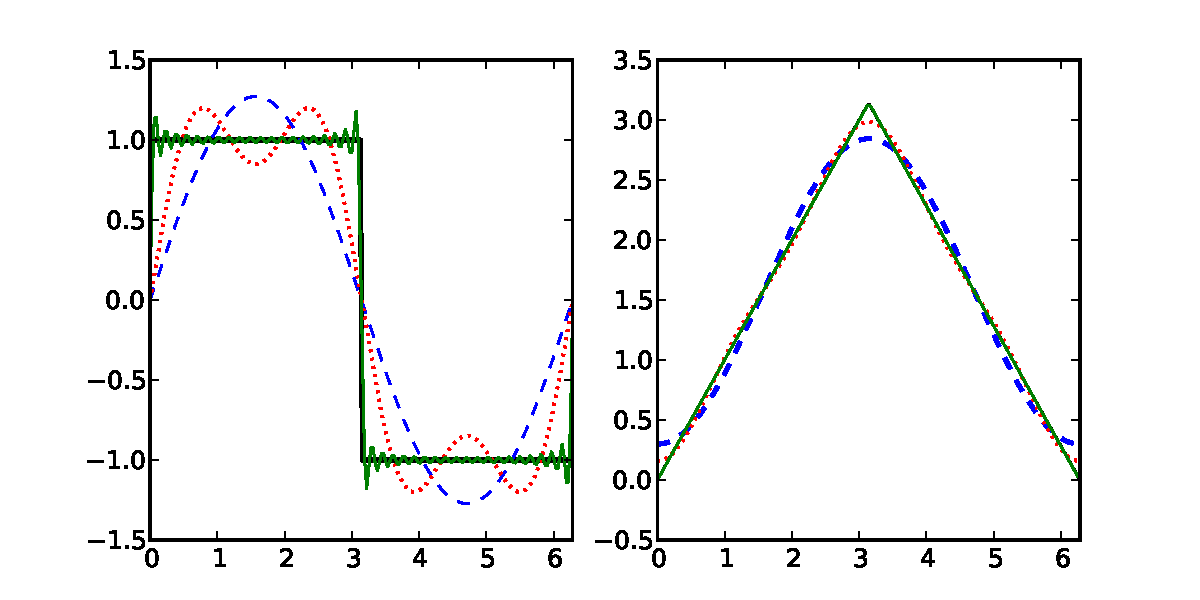
\includegraphics[width=\textwidth]{plots/fourier}
  \caption{Abgeschnittene Fourierreihen der Rechteckfunktion (links)
    und eines Dreieckpulses (rechts). Die Funktionen sind jeweils als
    schwarze durchgezogene Linien eingezeichnet, die Näherungen mit
    einem Term blau gestrichelt, mit zwei Termen rot gepunktet, und
    mit 20 Termen grün durchgezogen. Für den Dreieckpuls ist letztere
    Näherung nicht mehr von der Funktion zu unterscheiden, während der
    Rechteckpuls noch deutliche Artefakte an den Unstetigkeiten zeigt.}
  \label{fig:fourier}
\end{figure}
Einige reelle Fourierreihen sind zum Beispiel:
\begin{itemize}
\item Konstante $f(t) = f_0$:
  \begin{equation}
    a_0 = 2 f_0,\quad a_n,\,b_n= 0\quad\text{sonst}
  \end{equation}
\item Rechteckfunktion
  \begin{equation}
    f(t) = \begin{cases}
      1 &\text{für}\; 0 \le t < \frac{T}{2} \\
      -1  &\text{für}\; \frac{T}{2} \le t < T
    \end{cases}\\
    = \quad\frac{4}{\pi}\sum_{n=1}^\infty
    \frac{1}{2n-1}\sin\left((2n-1)\omega t\right)
  \end{equation}
\item kurzer Rechteckpuls. Wir betrachten nun die auf konstanten
  Flächeninhalt normierte Funktion
  \begin{equation}
    f_S(t) = \begin{cases}
      1/S &\text{für}\; 0 \le t < S \\
      0  &\text{für}\; S \le t < T
    \end{cases},
  \end{equation}
  deren Fourierreihe
  \begin{equation}
    f_s(t) =
    \quad \frac{1}{T} +
    \quad\frac{2}{T}\sum_{n=1}^\infty
    \frac{\sin(n\omega S)}{n\omega S}\cos(n\omega t) +
    \frac{1-\cos(n\omega S)}{n\omega S}\sin(n\omega t)
  \end{equation}
  ist. Je kleiner $S$ wird und damit der Träger von $f_S$, desto
  langsamer konvergiert ihre Fourierreihe, da die Funktion $\sin(x)/x$
  immer dichter an der Null ausgewertet wird. Für jede feste Frequenz
  $n$ gilt schließlich
  \begin{equation}
    \widehat{\left(f_S\right)}_n \xrightarrow{S\to 0} \frac{1}{T} = \hat\delta_n
    \quad\text{für alle}\;n\in\ZZ
  \end{equation}
  bzw.. $a_n\to 2/T$ und $b_n\to 0$. Die $\delta$-Funktion, die ja der
  formale Grenzwert der $f_S$ ist, und den kleinstmöglichen
  Träger hat, hat also in gewisser Weise die am schlechtesten
  (tatsächlich gar nicht!) konvergierende Fourierreihe.
\item Dreiecksfunktion
  \begin{equation}
    f(t) = \begin{cases}
      t      &\text{für}\; 0 \le t < \frac{T}{2} \\
      T - t  &\text{für}\; \frac{T}{2} \le t < T
    \end{cases}\quad=\quad\frac{\pi}{2} -
    \frac{4}{\pi}\sum_{n=1}^\infty
    \frac{1}{(2n-1)^2}\cos\left((2n-1)\omega t\right)
  \end{equation}
\end{itemize}
Genau wie die komplexe Fourierreihe lässt sich natürlich auch die
reelle Fourierreihe abschneiden, um Näherungen für Funktionen zu
bekommen, vergleiche Abbildung~\ref{fig:fourier}. Es fällt auf, das
die Fourierreihe besonders schlecht dort konvergieren, wo die Funktion
nicht differenzierbar ist bzw..\ einen Sprung aufweist.

\subsection{Diskrete Fouriertransformation}
\index{Fouriertransformation>diskrete}
\index{DFT}

\begin{figure}
  \centering
  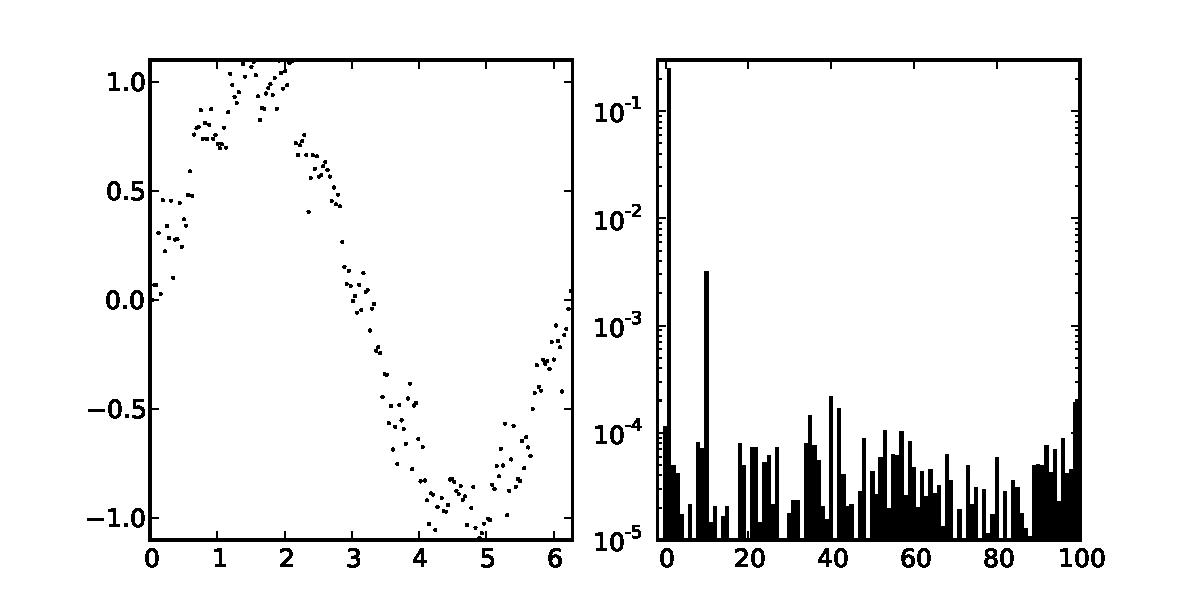
\includegraphics[width=\textwidth]{plots/fftsin}
  \caption{Diskrete Fouriertransformation von 200 diskreten
    Datenpunkten, die analog zu Abbildung~\ref{fig:leastsq} zwischen 0
    und $2\pi$ als $\sin(x) + 0,1\,sin(10 x) + \xi$ erzeugt wurden.
    Anders als der Funktionsfit erlaubt die DFT, auch die kleine
    zusätzliche Schwingung gut vom Rauschen zu unterscheiden. Im
    Graphen ist das Leistungsspektrum $\lvert DFT(k)\rvert^2$ gezeigt.
    Man erkennt die Amplitudenquadrate $0,25$ bei 1 und $0,01$ bei 10,
    auch wenn letztere Frequenz durch das Rauschen etwas an Intensität
    verloren hat.
  }
  \label{fig:fouriersin}
\end{figure}

\begin{figure}
  \centering
  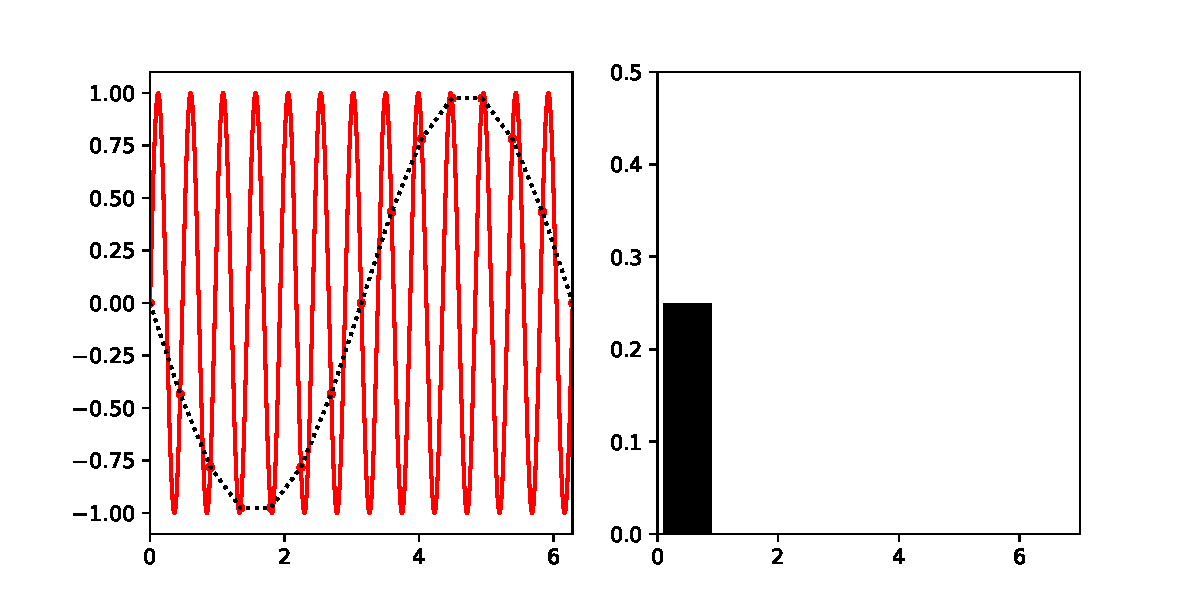
\includegraphics[width=\textwidth]{plots/fftalias}
  \caption{Diskrete Fouriertransformation von 14 äquidistanten
    diskreten Datenpunkten (rote Punkte links) der Funktion
    $\sin(13t)$ (rote Kurve links) im Interval $[0:2\pi]$.  Die
    Frequenz der Funktion $13/2\pi$ ist höher als die Nyquist-Frequenz
    $f_\text{Nyquist}=14/2\pi$, daher kommt es zu
    Aliasing-Artefakten. Die rekonstruierte Kurve ist links schwarz
    gepunktet eingezeichnet, ihr Spektrum rechts. Die abgetastete
    Funktion ist also scheinbar $\sin(t)$, was einer Frequenz von
    $2f_\text{Nyquist} - 13/2\pi$ entspricht.}
  \label{fig:fourieralias}
\end{figure}

Bei praktischen Anwendungen sind die Integrale zur Bestimmung der
Koeffizienten oft nicht analytisch lösbar, oder die Funktion ist von
vornherein nur an diskreten Punkten gegeben, etwa weil es sich um
Messdaten handelt. In diesem Fall müssen die Integrale numerisch
approximiert werden. Wir betrachten nun also nicht mehr eine
kontinuierliche Funktion $f$, sondern Daten $f_k = f(t_k)$ mit
$t_k=k\Delta$, $k=0(1)N-1$ und Schrittweite $\Delta =
\frac{T}{N}$. Dann ist
\begin{equation}
  \hat{f}_n = \frac{1}{T}\int_0^T f(t)e^{-i n\omega t}\, dt
  \approx
  \frac{\Delta}{T}\sum_{k=0}^{N-1} f(k\Delta) e^{-i n\omega k\Delta}
  =
  \frac{1}{N}\sum_{k=0}^{N-1} f_k e^{-i\frac{2\pi}{N} n k} =: \frac{g_n}{N}.
\end{equation}
Die Koeffizienten
\begin{equation}
  \label{eq:dft}
  \text{DFT}(f_k)_n = g_n = \sum_{k=0}^{N-1} f_k e^{-i \frac{2\pi}{N} n k}
\end{equation}
werden als die \emph{diskrete Fouriertransformierte} bezeichnet, die
sehr effizient berechnet werden kann, wie wir im folgenden sehen
werden. Analog wird die \emph{inverse diskrete Fouriertransformation}
\begin{equation}
  \label{eq:idft}
  \text{iDFT}(g_n)_k = f(t_k) = \sum_{n=0}^{N-1} \frac{g_n}{N} e^{i \frac{2\pi}{N} n k}
\end{equation}
definiert, die aus den Koeffizienten wieder die Funktion $f$ an den
diskreten Eingangspunkten $t_k$
berechnet. Abbildung~\ref{fig:fouriersin} zeigt zum die DFT der Summe
zweier verrauschter Sinusfunktionen, aus der die beiden
Basisfrequenzen und deren Amplituden klar gegenüber dem Rauschen zu
erkennen sind.

Die Koeffizienten sind offenbar periodisch, da
\begin{equation}
  \label{eq:dftper}
  g_{n+N} = \sum_{k=0}^{N-1} f_k e^{-i\frac{2\pi}{N} (n + N) k} =
  \sum_{k=0}^{N-1} f_k e^{-i\frac{2\pi}{N} n k} \underbrace{e^{-2\pi i k}}_{=1} = g_n.
\end{equation}
Insbesondere ist $g_{-k} = g_{N-k}$, und es gibt nur $N$ echt
verschiedene Koeffizienten bzw.. Frequenzen $n/T$. DFT-Bibliotheken
speichern die Koeffizienten daher meist als Vektor
$(g_{0},\ldots,g_{N-1})$
bzw.. $(g_{0},\ldots,g_{N/2-1},g_{-N/2},\ldots,g_{-1})$.  Ist $f$
reell, so gilt noch dazu $g_{-k} = \overline{g_{k}}$, sodass lediglich
$\lceil N/2\rceil$ Koeffizienten wirklich verschieden sind. Allerdings
sind diese im allgemeinen komplex, so dass die $N$ reellen
Freiheitsgrade der Eingangsfunktion erhalten bleiben.

% verhindert zwei ziemlich unterfüllte Seiten
\enlargethispage{\baselineskip}

Die endliche Anzahl der diskreten Fourierkoeffizienten bedeutet, dass
bei einem reellen Signal mit Schrittweite $\Delta$ die maximal
darstellbare Frequenz $f_\text{Nyquist}=\frac{1}{2\Delta}$ beträgt,
die sogenannte
\emph{Nyquist-Frequenz}\index{Nyquist-Frequenz}. Signale mit höherer
Frequenz $f$ werden zu scheinbaren Signalen niedrigerer Frequenz
\begin{equation}
  f_\text{scheinbar} = \begin{cases}
    f \bmod 2 f_\text{Nyquist} & \text{falls}\; f \bmod 2 f_\text{Nyquist}
    < f_\text{Nyquist} \\
    2f_\text{Nyquist} - f \bmod 2 f_\text{Nyquist} & \text{falls}\; f \bmod 2 f_\text{Nyquist}
    \ge f_\text{Nyquist},
  \end{cases}
\end{equation}
was auch als \emph{Aliasing} bezeichnet
wird. Sollen analoge Signale digital weiter verarbeitet werden, kann
es daher notwendig sein, höhere Frequenzen durch analoge
Tiefpassfilter zu unterdrücken. Abbildung~\ref{fig:fourieralias}
illustriert dieses Problem.

\subsection{Schnelle Fouriertransformation}
\index{Fouriertransformation>schnelle}\index{FFT}

Die Berechnung der Fouriertransformierten nach \eqref{eq:dft} ist zwar
möglich, aber ziemlich langsam --- jeder der $N$ Koeffizienten
benötigt offenbar $\O(N)$ Operationen, so dass die DFT insgesamt
$\O(N^2)$ Operationen braucht. Das limitiert für praktische
Anwendungen $N$ auf einige tausend, was für viele Anwendungen zu wenig
ist. Die DFT konnte daher nur durch die \emph{schnelle
  Fouriertransformation} (FFT) von \emph{Cooley und Tukey} zu breiter
Anwendung finden. Diese basiert auf der Beobachtung, dass für $N=2M$
\begin{align}
  \text{DFT}(f_k)_n &= \sum_{k=0}^{M-1} f_{2k} e^{-i\frac{2\pi}{2M} n\, 2k} +
  \sum_{k=0}^{M-1} f_{2k+1} e^{-i\frac{2\pi}{2M} n\, (2k + 1)}\\
  &= \text{DFT}(f_{2k})_n + e^{-i\frac{2\pi}{2M} n}
  \text{DFT}(f_{2k+1})_n,
\end{align}
wobei $\text{DFT}(f_{2k})_n$ den $n$-ten Koeffizienten einer DFT auf
den Datenpunkten $f_{2k}$, $k=0(1)M-1$, bezeichnet. Gemäß
\eqref{eq:dftper} ist dabei $\text{DFT}(f_{2k})_n =
\text{DFT}(f_{2k})_{n-M}$ für $n>M$.

Die Fouriertransformierte der $N$ Datenpunkte ergibt sich also als
einfache Summe von zwei
Fouriertransformierten mit lediglich der halben Menge $M$ an
Datenpunkten, wobei die ungerade Hälfte mit der \emph{Einheitswurzel}
\begin{equation}
  w^n := e^{-i\frac{2\pi}{2M} n}
\end{equation}
multipliziert wird.  Ist nun $M$ wieder durch zwei teilbar, so lassen
sich diese Fouriertransformierten ebenfalls als Summe zweier nochmals
halb so langer Fouriertransformationen darstellen. Wenn nun $N$ eine
Zweierpotenz ist, kann man so fortfahren, bis $M=1$ erreicht ist, also
$\text{DFT}(f_0)_0 = f_0$. Dabei gibt es offenbar $\log_2(N)$ viele
Unterteilungsschritte, die jeder $\O(N)$ Operationen kosten. Insgesamt
benötigt die FFT also lediglich $\O(N\log N)$ Operationen.

Schematisch funktioniert ein FFT-Schritt wie folgt:
\begin{center}
  \begin{tikzpicture}[x=2em,y=3em,>=stealth']
    \draw (0,0)  node (f0) {$f(0)$} ;
    \draw (0,-1) node (f1) {$f(\Delta)$} ;
    \draw (0,-2) node (f2) {$f(2\Delta)$} ;
    \draw (0,-3) node (f3) {$f(3\Delta)$} ;

    \draw (3,0.25) rectangle +(2,-1.5);
    \draw (4,-0.5) node {
      \begin{minipage}{4em}\centering
        Halbe\\
        FFT
      \end{minipage}
    } ;

    \draw (3,-1.75) rectangle +(2,-1.5);
    \draw (4,-2.5) node {
      \begin{minipage}{4em}\centering
        Halbe\\
        FFT
      \end{minipage}
    } ;

    \draw (8,0)  node (g0) {$g_0$} ;
    \draw (8,-1) node (g1) {$g_1$} ;
    \draw (8,-2) node (g2) {$g_2$} ;
    \draw (8,-3) node (g3) {$g_3$} ;

    \draw[->] (f0) -- (3,0);
    \draw[->] (f2) -- (3,-1);
    \draw[->] (f1) -- (3,-2);
    \draw[->] (f3) -- (3,-3);

    \draw[->] (5,0)   -- node[above,pos=0.97] {$\cdot 1$} (g0.west);
    \draw[->] (5,-2)  -- node[below,pos=0.97] {$\cdot w^0$}(g0.west);
    \draw[->] (5,-1)  -- node[above,pos=0.97] {$\cdot 1$}(g1.west);
    \draw[->] (5,-3)  -- node[below,pos=0.97] {$\cdot w^1$}(g1.west);
    \draw[->] (5,-2)  -- node[above,pos=0.97] {$\cdot 1$}(g2.west);
    \draw[->] (5,0)   -- node[below,pos=0.97] {$\cdot w^2$}(g2.west);
    \draw[->] (5,-3)  -- node[above,pos=0.97] {$\cdot 1$}(g3.west);
    \draw[->] (5,-1)  -- node[below,pos=0.97] {$\cdot w^3$}(g3.west);
  \end{tikzpicture}
\end{center}
Aufgrund ihres Aussehens wird dieses Datenpfadschema auch als
Butterfly-Schema genannt. Damit die beiden Unter-FFTs auf einem
zusammenhängenden Satz von Daten operieren können, müssen also auch
die Eingabedaten $f_k$ umsortiert werden, ebenso wie auch für die
Unter-FFTs. Man kann sich leicht überlegen, dass dabei $f_k$ auf
$f_{k'}$ sortiert wird, wobei die Bits  $k'$ in Binärdarstellung
dieselben wie von $k$ sind, nur in umgedrehter Reihenfolge.

Die FFT erlaubt also die effiziente Zerlegung einer Funktion in ihre
Schwingungskomponenten, was viele wichtige Anwendungen nicht nur in
der Physik hat. Daher gibt es eine Reihe sehr guter Implementierungen
der FFT, allen voran die "`Fastest Fourier Transform in the West"'
(FFTW, \url{http://www.fftw.org}). Selbstverständlich bietet auch NumPy
eine FFT, \scipy{numpy.fft.fft(f_k)}, mit der inversen FFT
\scipy{numpy.fft.ifft(g_n)}. Die Routinen sind so implementiert, dass
bis auf Maschinengenauigkeit $\text{iFFT}(\text{FFT}(f_k)) = f_k$.

Wichtige Anwendungsbeispiele der diskreten Fouriertransformation sind
zum Beispiel die Datenformate JPEG, MPEG und MP3, die alle drei auf
einer Abwandlung der DFT beruhen, der \emph{diskreten
  Cosinustransformation} (DCT) für reelle Daten. Bei dieser wird der
Datensatz so in der Zeitdomäne verdoppelt, dass er in jedem Fall eine
gerade Funktion repräsentiert, wodurch die Fourierreihe in eine reine
Cosinusreihe übergeht mit nur reellen Koeffizienten. Die DCT ist also
eine Umwandlung reeller in reelle Zahlen. Wegen Ihrer Wichtigkeit gibt
es nicht nur extrem effiziente Implementierungen für die meisten
Prozessortypen, sondern auch spezielle Hardware.

\section{\keyword{Wavelets}}
\index{Multiskalenanalyse}

Die Fouriertransformation wird vor allem deshalb für die Kompression
von Audio- oder Bilddaten genutzt, weil sie hochfrequente von
niederfrequenten Signalen trennt und die menschlichen Sinne die
hochfrequenten Anteil meist nicht gut wahrnehmen können. Das ist
allerdings nicht ganz korrekt, tatsächlich können wir nur stark lokale
Änderungen nicht gut wahrnehmen. Dafür sind Fourierreihen an sich gar
nicht so gut geeignet, da ja auch die hochfrequenten Schwingungen
alles andere als lokal sind. Als Alternative hat sich die
\emph{Multiskalenanalyse} (MSA) oder \emph{diskrete
  Wavelettransformation} etabliert, die auch im transformierten Raum
lokal ist.

\begin{figure}
  \centering
  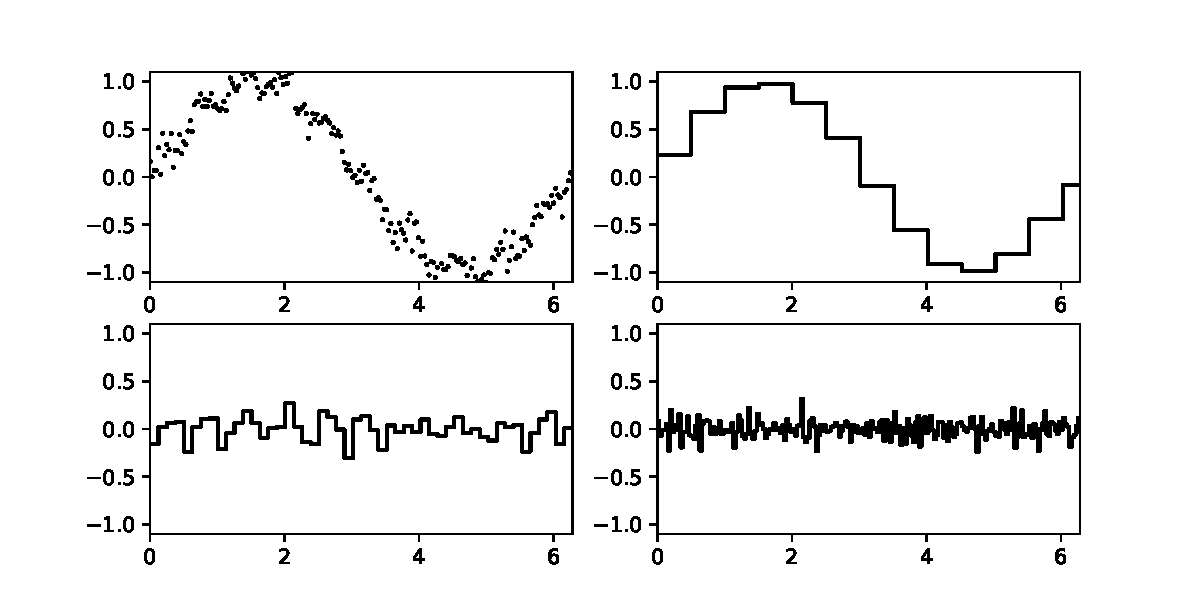
\includegraphics[width=\textwidth]{plots/wavelet}
  \caption{Diskrete Wavelettransformation von 200 diskreten
    Datenpunkten, die analog zu Abbildung~\ref{fig:fouriersin} zwischen
    0 und $2\pi$ als $\sin(x) + 0,1\,sin(10 x) + \xi$ erzeugt
    wurden. Für die Transformation wurden die Wavelets von $(0,1]$ auf
    den Bereich $(0,2\pi]$ gestreckt. Der linke obere Graph zeigt
    nochmals das Ausgangssignal, von rechts oben nach rechts unten
    folgen die Anteile der Stufen 0--3, also $(f,\phi_0)\phi_0 +
    \sum_{j=0}^{3} \sum_{k=0}^{2^j-1} (f,\psi_{jk})\psi_{jk}$, dann
    Stufen 4 und 5 ($\sum_{j=4}^{5} \sum_{k=0}^{2^j-1}
    (f,\psi_{jk})\psi_{jk}$) und schließlich Stufen 6--8, womit die
    Auflösung der Ausgangsdaten erreicht ist.}
  \label{fig:dwt}
\end{figure}

Anders als bei der Fouriertransformation, die eine Zerlegung in
trigonometrische Funktionen darstellt, gibt es für die MSA
verschiedene Sätze von Basisfunktionen mit verschiedenen Eigenschaften
wie Differenzierbarkeit und Lokalität. Im folgenden soll die MSA mit
Hilfe des Haar-Wavelets dargestellt werden, dass das einfachste und
älteste bekannte Wavelet ist. Zunächst betrachten wir die
\emph{Skalierungsfunktion}
\begin{equation}
  \phi(x) = \chi_{(0,1]} =
  \begin{cases}
    1 &\text{für}\; 0 < x \le 1\\
    0 &\text{sonst}
  \end{cases}
\end{equation}
sowie das Haar-\emph{Wavelet}
\begin{equation}
  \psi(x) =
  \begin{cases}
    -1 &\text{für}\; 0 < x \le \frac{1}{2}\\
    1 &\text{für}\; \frac{1}{2} < x \le 1 \\
    0 &\text{sonst},
  \end{cases}
\end{equation}
aus denen wir die Basisfunktionen $\phi_k(x) := \phi(x - k)$ der nullten
Stufe und $\psi_{jk}(x) := 2^{j/2}\psi(2^jx-k)$ der $j$-ten Stufe
konstruieren. Durch die Skalierung mit $2^j$ werden die $\psi_{j,k}$
also immer schmaler, sind aber wegen des Vorfaktors alle normiert,
d.h. $\lVert \psi_{jk} \rVert = 1$. Ebenso sind auch die $\phi_k$
normiert. Zusätzlich sind sämtliche Basisfunktionen zu einander
orthogonal, wie man sich leicht überlegt. Daher lässt sich jede
quadratintegrable Funktion $f$ wie folgt zerlegen:
\begin{equation}
  f(x) = \sum_{k\in\ZZ} (f,\phi_k)\phi_k + \sum_{j\in\NN_0}
  \sum_{k\in\ZZ} (f,\psi_{jk})\psi_{jk}
\end{equation}
Dies ist die Multiskalenanalyse von $f$. Die Koeffizienten der Stufe
$j$ werden auch Details der Stufe $j$ genannt. In der Praxis ist das
Signal durch endlich viele äquidistante Datenpunkte gegeben, analog
zur diskreten Fouriertransformation. In diesem Fall sind die Summen
endlich, da einerseits der Träger endlich ist und damit nur endlich
viele $(f,\phi_k)\neq 0$, und es andererseits keine Details unterhalb
der Auflösung des Signals gibt. Man skaliert dann die Wavelets und
Skalierungsfunktion so, dass der Abstand der Datenpunkte gerade der
halben Breite des Wavelets auf der feinsten Auflösung entspricht, und
$\phi = \phi_0$ bereits das gesamte Interval überdeckt. Für eine nur
auf $[0,1]$ nichtverschwindende Funktion, deren Werte an $2^N$ Punkten
äquidistanten Punkten bekannt ist, reduziert sich die
Multiskalenanalyse zur \emph{diskreten
  Wavelettransformation}\index{Wavelets>-transformation}
\begin{equation}
  \label{eq:idwt}
  f(x) = (f,\phi)\phi +
  \sum_{j=0}^{N-1} \sum_{k=0}^{2^j-1} (f,\psi_{jk})\psi_{jk}.
\end{equation}
Die Anzahl der Koeffizienten ist dann $1 + 1 + 2 + \cdots + 2^{N-1} =
2^N$, also genau die Anzahl der Eingabedaten. Genau wie die diskrete
Fouriertransformation bildet die Wavelettransformation $2^N$ Werte
$f(k/2^N)$ auf $2^N$ Werte $(f,\phi)$ und $(f,\psi_{jk})$ ab und
besitzt eine exakte Rücktransformation, \eqref{eq:idwt}.

Analog zur schnellen Fouriertransformation gibt es auch eine schnelle
Wavelettransformation (FWT), die sogar linearen Aufwand hat, also $\O(N)$
Schritte bei $N$ Datenpunkten benötigt. Eine einfache Implementation
der FWT und der inversen FWT für das Haar-Wavelet zeigt
Codebeispiel~\ref{lst:dwt}. Der Kern dieser Transformation liegt
darin, die Transformierte von der höchsten Detailauflösung herab
aufzubauen, und dadurch die die Integrale approximierenden Summen
schrittweise aufzubauen (\emph{Downsampling}). Für genauere
Informationen siehe zum Beispiel \textcite{daubechies92a}.

Abbildung~\ref{fig:dwt} zeigt einige Detailstufen der
Wavelet-Zerlegung der verrauschten Sinusfunktionen analog
Abbildung~\ref{fig:fouriersin}. Auch hier lässt sich das Rauschen auf
den höheren Detailstufen gut vom Nutzsignal trennen, allerdings kann
die Oberschwingung nicht detektiert werden. Das hängt allerdings vor
allem daran, dass das Haar-Wavelet nicht sehr geeignet ist, da es
nicht glatt ist, im Gegensatz zum Nutzsignal. Daher sind in den
meisten Fällen glatte Wavelets besser geeignet. Das bekannteste
Beispiel von glatten Wavelets sind die Daubechies-Wavelets, die
daneben auch einen kompakten Träger haben, also stark lokalisiert
sind. Mit solchen Wavelets lassen sich sogar reale Musikdaten in
Akkorde zurücktransformieren. Auch der JPEG-Nachfolger JPEG2000
basiert auf einer Wavelettransformation statt einer
Cosinustransformation, allerdings mit
Cohen-Daubechies-Feauveau-Wavelets.

\lstinputlisting[style=floating,firstline=10,
caption={Diskrete Wavelettransformation und ihre Inverse als
  Python-Code. Die Länge der Eingabedaten muss eine Zweierpotenz $2^N$
  sein. Die Details sind in einem Vektor $c$ gespeichert, in der Form
  $c=((f,\phi_0)$, $(f, \psi_{00})$, $(f, \psi_{10})$, $(f, \psi_{11})$,
  $(f, \psi_{20})$, $(f, \psi_{21})$, $(f, \psi_{22}), \ldots,
  (f, \psi_{N-1,2^{N-1}-1}))$.
},
label=lst:dwt]{dwt.py}

%%% Local Variables: 
%%% mode: latex
%%% TeX-master: "padc"
%%% TeX-PDF-mode: t
%%% End: 

% Dies ist Teil der Vorlesung Physik auf dem Computer, SS 2012,
% Axel Arnold, Universitaet Stuttgart.
% 
% Dieses Werk ist unter einer Creative Commons-Lizenz vom Typ
% Namensnennung-Weitergabe unter gleichen Bedingungen 3.0 Deutschland
% zugänglich. Um eine Kopie dieser Lizenz einzusehen, konsultieren Sie
% http://creativecommons.org/licenses/by-sa/3.0/de/ oder wenden Sie sich
% schriftlich an Creative Commons, 444 Castro Street, Suite 900, Mountain
% View, California, 94041, USA.

\chapter{Datenanalyse und Signalverarbeitung}

In diesem Kapitel geht es darum, was man mit einem gemessenen Signal
machen kann und muss. Ein gemessenes Signal kann dabei entweder
tatsächlich von einem Messgerät kommen oder aber das Ergebnis einer
Computersimulation sein. Zwei Fragen sind dabei vor allem wichtig:
Welche Eigenschaften hat das Signal, und wie vertrauenswürdig sind die
Werte?

Um die Eigenschaften von Signalen zu untersuchen, ist die
kontinuierliche Fourieranalyse ein gutes Werkzeug, die das Signal vom
Zeit- in den Frequenzraum überträgt. So lassen sich zum Bespiel
charakteristische Frequenzen und damit Zeitskalen bestimmen. Außerdem
bietet der Übergang in den Frequenzraum analytisch viele Vorteile, die
sich auch auf dem Computer nutzen lassen. So werden zum Beispiel
langreichweitige Wechselwirkungen in Molekulardynamiksimulationen
meist im Frequenzraum berechnet.

Als weiteres Werkzeug werden wir Faltungen kennen lernen, die
erlauben, Signale nach bestimmten Frequenzen zu filtern oder aber aus
der (gemessenen) Antwort eines linearen Systems auf ein einfaches
Eingangssignal die Antwort auf beliebige Signale zu berechnen.

Sollen Signale mit dem Computer weiterverarbeitet werden, müssen diese
\emph{digitalisiert} werden, also in eine Reihe von Zahlen
übersetzt. Üblicherweise passiert dies dadurch, dass das Signal nur zu
äquidistanten Zeitpunkten ausgewertet, \emph{abgetastet} wird. Das
wirft die Frage auf, welche Funktionen dadurch überhaupt gut gemessen
werden können. Wie wir sehen werden, beschränkt diese Abtastung die
Frequenzen, die von einer digitalen Auswertung erfasst werden können.

Die meisten Signale sind außerdem, durch Messungenauigkeiten und
prinzipielle stochastische Prozesse, selbst \emph{stochastisch},
\dh die Verteilung der Ergebnisse vieler Messungen ist
vorherbestimmbar, die einzelne Messung hingegen nicht. Trotzdem sind
Messungen oft korreliert, zum Beispiel weil eine Observable sich nur
kontinuierlich ändert.  Durch Korrelationsanalysen lässt sich
bestimmen, wann Messungen wirklich unabhängig sind. Dies gibt wiederum
Aufschluss über die Zeitskalen wichtiger Prozesse im System, ist aber
auch wichtig für eine korrekte Abschätzung des Messfehlers, womit sich
der letzte Abschnitt beschäftigt.

\section{Kontinuierliche Fouriertransformation}
\index{Fouriertransformation>kontinuierliche}

Für die Analyse zeitlich veränderlicher Signale besonders nützlich ist
die Fouriertransformation, die ein kontinuierliches Signal in den
Frequenzraum übersetzt. Dies gilt nicht nur für periodische Signale,
sondern zum Beispiel auch dann, wenn die Antwort eines Systems auf ein
komplexes Eingangssignal gefragt ist. Der tiefere Grund dafür ist,
dass die Fouriertransformation Differential- und Integraloperatoren in
einfache algebraische Operationen übersetzt.

Betrachten wir nochmals die Fourierreihe im Interval $[-T/2,T/2)$
\begin{multline}
  f(t) = \sum_{n\in\ZZ}
  \left(\frac{\Delta\omega}{2\pi}\int_{-T/2}^{T/2}
    f(t)e^{-i n\Delta\omega t}\, dt\right)
  e^{i n\Delta\omega t}\\
  =
  \frac{1}{\sqrt{2\pi}}\sum_{n\in\ZZ}
  \left(\frac{1}{\sqrt{2\pi}}\int_{-T/2}^{T/2} f(t)e^{-i \omega t}\,dt\right)
  e^{i \omega t}\,\Delta\omega
\end{multline}
mit der Grundfrequenz $\Delta\omega=2\pi/T$ und
$\omega=n\Delta\omega$. Im Grenzwert $T\to\infty$ ergibt sich
\begin{equation}
  \label{eq:contfourierinverse}
  f(t) = \frac{1}{\sqrt{2\pi}}\int_{-\infty}^{\infty}
  \FT(f)(\omega)e^{i \omega t}\,d\omega
\end{equation}
mit
\begin{equation}
  \label{eq:contfourier}
  \FT(f)(\omega) =
  \frac{1}{\sqrt{2\pi}}\int_{-\infty}^{\infty} f(t)e^{-i \omega t}\, dt.
\end{equation}
Die \emph{kontinuierliche Fouriertransformation} $\FT$ ist das
Analogon der periodischen Fourierreihe, ist allerdings keine
Transformation in eine Reihe mehr, sondern eine Abbildung zwischen
Funktionen. Für $\FT$ gelten eine Menge sehr starker Aussagen, die wir
zum großen Teil in ähnlicher Art schon von der Fourierreihe kennen:
\begin{itemize}
\item $\FT(f)$ existiert, falls $f$ quadratintegrabel ist, und
  bildet $f$ auf eine quadratintegrable Funktion ab. Für solche
  Funktionen mit der zugehörigen Norm $\lVert f \rVert_2 =
  \int_{-\infty}^{\infty} \lvert f(t) \rvert^2\,dt$ gilt dann sogar
  die Isometrie
  (\emph{Parsevaltheorem}\index{Parsevaltheorem>kontinuierliches}):
  \begin{equation}
    \lVert \FT(f) \rVert_2 = \lVert f \rVert_2
  \end{equation}
\item $\FT$ ist linear, \dh $\FT(f + \lambda g) = \FT{f} + \lambda
  \FT{g}$.
\item $\FT$ ist reziprok gegen Streckungen, \dh
  \begin{equation}
    \label{eq:fourierreziprok}
    \FT[f(\alpha
    t)](\omega) = \frac{1}{\lvert \alpha \rvert}
    \FT(f)\left(\frac{\omega}{\alpha}\right).
  \end{equation}
  Wird also eine Funktion $\alpha$ immer stärker gestaucht, so wird
  ihre Transformierte immer weiter gestreckt.  Entsprechend wird aus
  Zeitumkehr Frequenzumkehr: $\FT(f(-t))(\omega) = \FT(f)(-\omega)$.
\item $\FT$ ist invertierbar, die Umkehrfunktion $\FT^{-1}$ ist durch
  \eqref{eq:contfourierinverse} explizit gegeben. Offenbar ist auch
  die Umkehrung eine Isometrie, es gilt $\lVert \FT^{-1}(f)
  \rVert_2 =\lVert f \rVert_2$.
\item Weiter gilt $\FT(\FT(f(t))) = f(-t)$, und damit $\FT^4(f) =
  f$. Insbesondere ist auch $\FT^{-1} = \FT^3$. Die
  Fouriertransformation ist damit eine vierte Einheitswurzel auf dem
  Raum der quadratintegrablen Funktionen, ähnlich wie $i$ bei den
  komplexen Zahlen.
\item Eine zeitliche Verschiebung wird zu einer Frequenzmodulation und
  umgekehrt:
  \begin{eqnarray}
    \label{eq:fouriertimeshift}
    \FT(f(t-t_0))(\omega) = e^{-i\omega t_0} \FT(f(t))(\omega)\\
    \label{eq:fourierfreqshift}
    \FT(e^{i\omega_0 t}f(t))(\omega) = \FT(f(t))(\omega-\omega_0).
  \end{eqnarray}
  Wird also ein niederfrequentes Signal (Radioprogramm) auf ein
  hochfrequentes Trägersignal aufmoduliert, verschiebt sich nur dessen
  Spektrum. 
\item Aus der Linearität folgt, dass stets gilt:
  $\FT(\overline{f})(\omega) = \overline{\FT(f)(\omega)}$.
\item Ist Funktion $f$ gerade (symmetrisch), also $f(t) = f(-t)$, so ist
  $\FT(f)(-\omega) = \FT(f)(\omega)$, also gerade (symmetrisch).
\item Ist Funktion $f$ ungerade (antisymmetrisch), also $f(t) = -f(-t)$, so ist
  $\FT(f)(-\omega) = -\FT(f)(\omega)$, ungerade (antisymmetrisch).
\item Ist Funktion $f$ reellwertig, also $f(t) = \overline{f(t)}$, so
  ist $\FT(f)(-\omega) = \overline{\FT(f)(\omega)}$, aber im
  allgemeinen komplexwertig!
\item Für die Fouriertransformierte der Ableitung gilt
  \begin{equation}
    \begin{split}
      \FT\left(\frac{d}{dt}f(t)\right)(\omega) &=
      \frac{1}{\sqrt{2\pi}}\int_{-\infty}^{\infty}
      \left[\frac{df}{dt}(t)\right]e^{-i
        \omega t}\, dt\\
      &\substack{=\\\text{part. Int.}} -\frac{1}{\sqrt{2\pi}}\int_{-\infty}^{\infty}
      f(t)\frac{d}{dt}e^{-i \omega t}\, dt = i\omega
      \FT(f(t))(\omega).
    \end{split}
  \end{equation}
  Dies spielt eine wichtige Rolle beim Lösen von
  Differenzialgleichungen, weil diese in gewöhnliche algebraische
  Gleichungen übergehen.
\item Es gilt die Poissonsche Summenformel
  \begin{equation}
    \label{eq:poissonsumme}
    \sum_{k\in\ZZ}f(t_0 + k\, \delta)=
    \frac{\sqrt{2\pi}}{|\delta|}\sum_{n\in\ZZ}\FT(f)
    \left(\frac{2\pi n}{\delta}\right)
    \exp\left(i \frac{2\pi n}{\delta} t_0\right).
  \end{equation}
  Diese Gleichung beruht darauf, dass $\sum_{t\in\ZZ}f(\cdot + t\,
  \delta)$ eine $\delta$-periodische Funktion ist, die durch eine
  Fourierreihe dargestellt werden kann. Wegen
  \eqref{eq:fouriertimeshift} reicht es
  dabei o.B.d.A. $\delta=1$ zu
  betrachten:
  \begin{multline}
    \sum_{k\in\ZZ}f(t_0 + k) =
    \sum_{n\in\ZZ} \int_0^1 \sum_{k\in\ZZ}f(\tau + k)e^{-2\pi i
      n \tau}\, d\tau
    \, e^{2\pi i n t_0} =\\
    \sum_{n\in\ZZ} \int_{-\infty}^\infty f(\tau)e^{-2\pi i
      n \tau}\, d\tau
    \, e^{2\pi i n t_0}
    = \sqrt{2\pi}\sum_{n\in\ZZ}\FT(f)(2\pi n)\, e^{2\pi i n t_0}.
  \end{multline}

  Eine wichtige Anwendung der Poissonschen Summenformel ist die
  Summation schlecht konvergenter Reihen. Fällt die Funktion $f$ sehr
  langsam gegen unendlich ab, so fällt ihre Fouriertransformierte
  wegen der Reziprozität \eqref{eq:fourierreziprok} im Allgemeinen
  schneller, so das aus einer langsam eine rasch konvergierende Reihe
  wird.
\end{itemize}

\subsection{Spezielle Fouriertransformierte}

Die Fouriertransformierte einer Gaußglocke ist
\begin{equation}
  \FT\left(\frac{1}{\sqrt{2\pi}}e^{-t^2/2}\right)
  =
  \frac{1}{2\pi}e^{-\omega^2/2}\int_{-\infty}^{\infty} e^{-(t-i\omega)^2/2}\, dt
  =
  \frac{1}{\sqrt{2\pi}}e^{-\omega^2/2}
\end{equation}
Die Gaussglocke ist also eine Eigenfunktion der Fouriertransformation
zum Eigenwert 1. Die Fouriertransformation hat tatsächlich sehr viel
mehr echt verschiedene Eigenfunktionen, die Familie der
Hermitefunktionen~\cite{pinsky02a}. Wegen $\FT^4=1$ kann die
Fouriertransformation nur die vier Eigenwerte $\pm 1$ und $\pm i$
haben. Jeder dieser Eigenwerte ist stark degeneriert, also der
Eigenraum zu jedem Eigenwert unendlichdimensional.

Die (formale) Fouriertransformierte der $\delta$-Funktion ist
\begin{equation}
  \label{eq:fourierdelta}
  \FT(\delta(t))(\omega)
  =
  \frac{1}{\sqrt{2\pi}}\int_{-\infty}^{\infty}
  \delta(t)e^{-i \omega t}\, dt = \frac{1}{\sqrt{2\pi}},
\end{equation}
also einfach die konstante Funktion $1/\sqrt{2\pi}$, die ebensowenig
wie die $\delta$-Funktion eine quadratintegrable Funktion
ist. Alternativ lässt sich die Beziehung aus der
Fouriertransformierten der Gaußglocke mit sinkender Varianz herleiten.

\subsection{Numerische kontinuierliche Fouriertransformation}
\label{sec:contdft}

Um die Eigenschaften der kontinuierlichen Fouriertransformation
numerisch zu nutzen, machen wir den Grenzübergang $T\to\infty$
rückgängig und ziehen uns auf ein für die betrachtetete Funktion
hinreichend großes $T$ zurück, so dass $\int_{\lvert t\rvert>T}\lvert
f(t)\rvert^2\, dt$ hinreichend klein ist. Das geht insbesondere, wenn
das Signal endlichen Träger hat, wie das bei echten gemessenen
Signalen stets der Fall ist.

Wir betrachten nun als Signal eine Funktion $f$, die wir nur an auf
einem äquidistanten Gitter $t_k = t_0 + k\frac{T}{N}$, $k=0(1)N-1$
kennen, also im Intervall $[t_0, t_o + T]$. Dann setzen wir
$\omega_0:=\frac{2\pi}{T}$ und $\Delta := \frac{T}{N}$, und erhalten
für ganzzahliges $n$
\begin{multline}
  \label{eq:dftcont}
  \FT(f)(\omega_0 n)\approx
  \frac{1}{\sqrt{2\pi}}\int_{t_0}^{t_0 + T} f(t)e^{-i n \omega_0 t}\, dt
  \approx
  \frac{1}{\sqrt{2\pi}}\sum_{k=0}^{N-1}
  \Delta f(t_k)
  e^{-i n\omega_0 \left(t_0 + k\Delta\right)}\,
  \\
  =   \Delta \frac{e^{-i n\omega_0 t_0}}{\sqrt{2\pi}}\sum_{k=0}^{N-1}
  f(t_k) e^{-2\pi i n k / N}\,
  =\frac{T}{N}\frac{\left(e^{-i\omega_0 t_0}\right)^n}{\sqrt{2\pi}} \text{DFT}(f(t_k))_n\,,
\end{multline}
wobei DFT die diskrete Fouriertransformation aus \eqref{eq:dft}
bezeichnet. Meist werden Messungen bei $t=0$ begonnen, die Funktion
ist dann nur im positiven Halbinterval von Null verschieden.  In
diesem Fall wählt man natürlicherweise $t_0 = 0$, so dass der Faktor
$e^{-i\omega_0 t_0} = 1$ entfällt. Wir werden allerdings später noch
Faltungen kennenlernen, bei denen es häufig natürlicher ist, eine
symmetrische Lage der Filterfunktion um die Null anzunehmen. In diesem
Fall wählt man $t_0 = -T/2$, so dass $e^{-i\omega_0 t_0} = -1$.

Die Koeffizienten der DFT sind periodisch, daher auch diese Näherung
für $\FT(f)$. Tatsächlich sollten die Koeffizienten aber nur als
Frequenzen im Interval $[-\omega_0 N/2,\omega_0 N/2]$ interpretiert
werden, alle Frequenzen außerhalb dieses Intervals sollten als Null
angesehen werden. Der Grund dafür ist das Abtasttheorem, dass im
folgenden Abschnitt besprochen wird. Dieses besagt, dass bei einem
Zeitschritt $\Delta=T/N$ nur Kreisfrequenzen bis $\omega_0 N/2 =
\pi/\Delta$ eindeutig gemessen werden können. Daher ist die
Beschränkung auf das innerste Interval die natürliche
Interpretation. Bei rein reellen Signalen ist es daher günstiger,
direkt die reellen Varianten der FFT-Implementationen zu nutzen, die
von vorneherein nur die relevanten positiven Koeffizienten bis $N/2$
zurückgeben.

Die Einschränkung der Frequenzen ist besonders wichtig, wenn $N$
ungerade ist und die um Null symmetrische Lage von $-T/2$ bis $T/2$
gewählt wird. Dann ist $\left(e^{-i\omega_0 t_0}\right)^{N-n} =
(-1)^{N-n} = - (-1)^{-n} = -\left(e^{-i\omega_0 t_0}\right)^{-n}$. Mit
anderen Worten, wird einfach die gesamte diskrete
Fouriertransformierte mit $(-1)^n$ multipliziert, so bekommen die
negativen Frequenzen das falsche Vorzeichen. Das hat drastische
Konsequenzen: wenn die Ursprungsfunktion reell ist, gilt
$DFT(f_k)_{-n}=\overline{DFT(f_k)}_{n}$, für die genäherte
kontinuierliche Fouriertransformierte also
$\FT(f)(-\omega)=-\overline{\FT(f)(\omega)}$. Das entspricht der
Tranformierten einer rein imaginären Funktion!

Analog wie die Fouriertransformation selber lässt sich auch ihre
Rücktransformation nähern:
\begin{equation}
  \label{eq:idftcont}
  \FT^{-1}(f)(t_k)\approx
  \text{iDFT}\left(\sqrt{2\pi}\frac{N}{T}\left(e^{i\omega_0 t_0}\right)^n f_n\right)_k
\end{equation}
Der Faktor $\left(e^{i\omega_0 t_0}\right)^n$ invertiert genau den
Faktor $\left(e^{-i\omega_0 t_0}\right)^n$ der
Vorwärtstransformation. Für $t_0=0$ ist er wieder 1 und muss nicht
berücksichtigt werden, bei $t_0=-T/2$ ist er $(-1)^n$.

Die bekannten schnellen FFT-Routinen lassen sich also auch für die
numerische Bearbeitung der kontinuierlichen Fouriertransformation
nutzen. Auf diese Weise ist \zb Abbildung~\ref{fig:fourierfaltung}
entstanden.

\subsection{\keyword{Abtasttheorem}}

In der Praxis sind Signale meist als diskrete Werte an (endlich
vielen) äquidistanten Stellen beziehungsweise Zeitpunkten gegeben, zum
Beispiel, weil ein Messgerät Daten in regelmäßigen Abständen liefert.
Eine wichtige Frage ist, wie gut man das reale Signal und sein
Frequenzspektrum aus den diskreten Datenpunkten rekonstruieren kann.

Hierzu betrachten wir zunächst ein \emph{bandbreitenbeschränktes
  Signal} $f$, \dh ein Signal, dessen Fouriertransformierte einen
kompakten Träger $[-\omega_\text{max},\omega_\text{max}]$ hat. Dann besagt die
Poissonsche Summenformel~\eqref{eq:poissonsumme}, dass für
$\omega\in[-\omega_\text{max},\omega_\text{max}]$
\begin{equation}
  \FT(f)(\omega) =
  \sum_{k\in\ZZ}\FT(e^{-i\omega \cdot} f)\left(2k\omega_0\right)
  =
  \frac{1}{\sqrt{2\pi}}
  \sum_{n\in\ZZ} e^{-i \omega n \Delta}f\left(n \Delta\right)
\end{equation}
mit $\Delta=\pi/\omega_\text{max}$. Die Fouriertransformierte eines
bandbreitenbeschränkten Signals lässt sich also \emph{exakt} nur aus
den Funktionswerten an den äquidistanten diskreten Stellen mit
Abtastrate $\Delta$ berechnen. Dadurch kann natürlich auch die
Funktion exakt aus ihrer Fouriertransformierten rekonstruiert werden:
\begin{equation}
  \label{eq:ftreconst}
  f(t)
  = \frac{\Delta}{2\pi}\sum_{n\in\ZZ} f\left(n \Delta\right)
  \int_{-\omega_\text{max}}^{\omega_\text{max}} e^{-i \omega (t - n\Delta)} \,d\omega
  = \frac{\Delta}{\pi}\sum_{n\in\ZZ} f\left(n \Delta\right)
  \frac{\sin(\omega_\text{max}(t-n\Delta))}{t-n\Delta}.
\end{equation}

Ist nun umgekehrt ein Signal $f$ an äquidistanten diskreten Stellen
$n\Delta$ gegeben, so lässt sich diesem gemäß \eqref{eq:ftreconst} ein
kontinuierliches Signal zuordnen, dessen Fouriertransformierte nur in
$[-\omega_\text{max},\omega_\text{max}]$ nicht verschwindet, wobei $\omega_\text{max} =
\pi/\Delta$. Das bedeutet, dass bei Abtastrate $\Delta$ nur Frequenzen
bis zur Nyquist-Frequenz $f_\text{Nyquist}=\frac{1}{2\Delta} =
\frac{\omega_\text{max}}{2\pi}$ eindeutig abgetastet werden können, ähnlich wie
im periodischen Fall.

\section{Faltungen}
\index{Faltung}

Die \emph{Faltung} der quadratintegrablen Funktionen $f$ und $g$ ist
definiert als
\begin{equation}
  (f \star g)(t) := \int_{-\infty}^{\infty} f(t')g(t-t')\,dt'.
\end{equation}
Das negative Vorzeichen von $t'$ in der zweiten Funktion sorgt
dafür, dass die Faltung kommutativ ist. Weitere Eigenschaften der
Faltung sind Linearität in den Komponenten und sogar
Assoziativität. Die Faltung verhält sich also so ähnlich wie die
klassische Multiplikation und wird daher mit dem Zeichen $\star$
bezeichnet.  Vereinfacht gesagt, deponiert die Faltung an jedem Punkt
$t$ die Funktion $f$, skaliert mit $g(\cdot - t) $. Daher ist \zb
\begin{equation}
  (\delta(\cdot - t_0) \star g)(t) = g(t - t_0).
\end{equation}
\index{Glättung}
Wird nun statt der unendlich dünnen $\delta$-Funktion zum Beispiel
eine Gaußglocke gewählt, so wird die Funktion $g$ verschmiert
bzw.\ geglättet, siehe Abbildung~\ref{fig:fourierfaltung}.

\begin{figure}
  \centering
  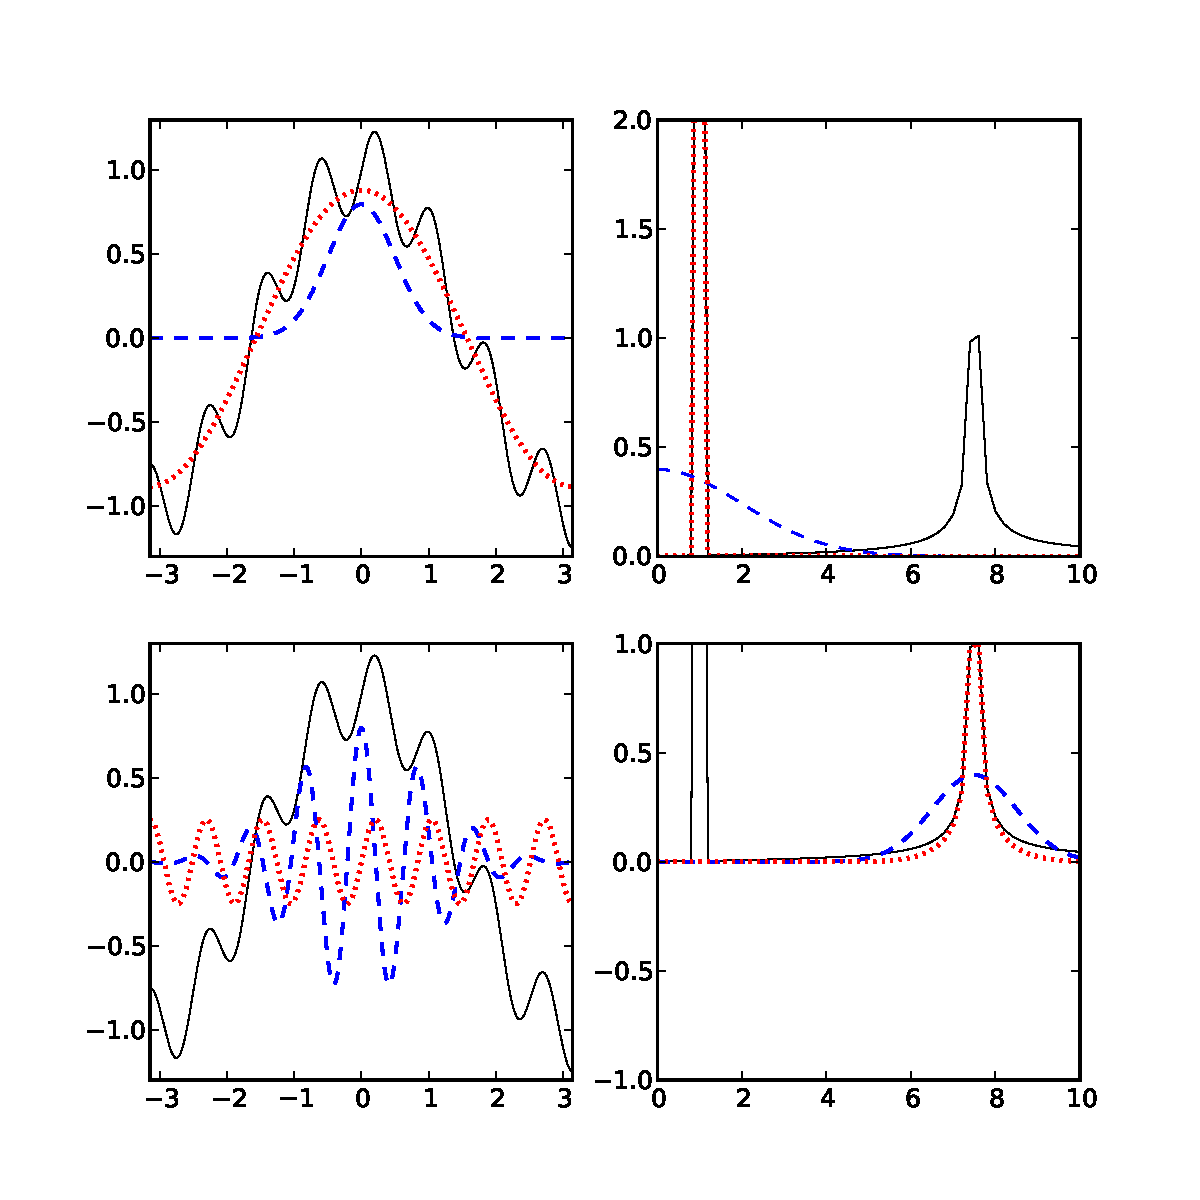
\includegraphics[width=\textwidth]{plots/fouriertrafo}
  \caption{Oben links: Summe zweier Schwingungen $\cos(x) +
    0,25\sin(7,5 x)$ (schwarze Linie), die mit einer Gaußglocke (blau
    gestrichelt) gefaltet wird. Das Ergebnis (rote gepunktete Linie)
    ist die quasi ungestörte langsame Schwingung ohne die
    höherfrequente Schwingung, die weggeglättet wurde. Oben rechts:
    Fouriertransformierte der Funktionen. Klar sichtbar ist die
    hochfrequente Störung mit einer Frequenz von $7,5$, die im
    gefilterten Signal fehlt. In der unteren Reihe wurde eine
    frequenzverschobene Gaußglocke benutzt, um statt der langsamen die
    schnelle Schwingung zu filtern; die Farbcodierung ist wie
    oben. Gemäß \eqref{eq:fourierfreqshift} bewirkt die
    Frequenzverschiebung eine Modulation der Gaußfunktion.}
  \label{fig:fourierfaltung}
\end{figure}

Die Fouriertransformierte der Faltung zweier Funktionen ist
\begin{equation}
  \label{eq:fourierfaltung}
  \begin{split}
    \FT(f\star g)(\omega) &=
    \frac{1}{\sqrt{2\pi}}\int_{-\infty}^{\infty}
    \int_{-\infty}^{\infty} f(t')g(t-t')\,dt' e^{-i \omega t}\,
    dt\\
    &= \frac{1}{\sqrt{2\pi}}\int_{-\infty}^{\infty}
    \int_{-\infty}^{\infty} f(t') g(t) e^{-i \omega (t+t')}\, dt\,
    dt'\\
    &= \frac{1}{\sqrt{2\pi}} \int_{-\infty}^{\infty} f(t')e^{-i
      \omega t'}\, dt' \int_{-\infty}^{\infty} g(t) e^{-i \omega
      t}\, dt = \sqrt{2\pi}\FT(f)(\omega)\FT(g)(\omega).
  \end{split}
\end{equation}
Die Faltung geht also in eine punktweise Multiplikation über. Im
Fourierraum lässt sich also sehr viel schneller falten, als im
Realraum, wo ja für jeden Punkt ein Integral zu lösen ist.

Dies nutzt man auch numerisch, um Faltungen zu berechnen, in
Verbindung mit \eqref{eq:dftcont}. Seien zwei Sätze mit $N$ Datenpunkten $f_k =
f(t_k)$  mit $t_k = t_0 + k\frac{T}{N}$  und $g_k = g(t'_k) $ mit
$t'_k = t'_0 + k\frac{T}{N}$ gegeben. Mit anderen Worten, die beiden
Funktionen müssen mit der selben Frequenz abgetastet worden sein, der
Anfangszeitpunkt kann aber verschieden sein. Das ist etwa beim
Glätten wichtig, bei dem die Filterfunktion meist symmetrisch um die
Null definiert ist, die zu glättende Funktion aber beliebig liegen
kann. Es gilt
\begin{multline}
  \label{eq:discretefold}
  (f\star g)(t_k) =
  \sqrt{2\pi}\FT^{-1}\left(\FT(f)(\omega)\FT(g)(\omega)\right)(t_k)\\
  \approx
  iDFT\left(2\pi \frac{N}{T} \left(e^{i\omega_0 t_0}\right)^n
  \left[\frac{T^2}{2\pi N^2}\left(e^{-i\omega_0 t_0}\right)^n\text{DFT}(f_k)_n\left(e^{-i\omega_0 t'_0}\right)^n\text{DFT}(g_k)_n\right]\right)_k\\
  =
  \frac{T}{N} \text{iDFT}\left[\left(e^{-i\omega_0 t'_0}\right)^n DFT(f_k)_n DFT(g_k)_n\right]_k.
\end{multline}
Wie im Abschnitt~\ref{sec:contdft} besprochen, muss $n$ als Frequenz
im Bereich $-N/2$ bis $N/2$ interpretiert werden. Man beachte, dass
der Faktor $\left(e^{-i\omega_0 t'_0}\right)^n$ nur durch den Aufpunkt
$t'_0$ der Abtastung der Funktion $g$ bestimmt ist, da wir an den
Stellen $t_k$ auswerten. Dadurch ist die Funktion $g$ die
Filterfunktion, die auf $f$ angewendet wird. Ist $g$ wie üblich
symmetrisch um Null abgetastet, so ist $\left(e^{-i\omega_0
    t'_0}\right)^n=(-1)^n$. Vergisst man diesen Term, entspricht das
einem impliziten Verschieben der Filterfunktion zur Null hin.
Die Lage $t_0$ der Abtastung der Funktion $f$ kann hingegen beliebig
verschoben sein. Die Faltung wird in jedem Fall natürlich nur im
Abtastbereich der Funktion $f$ berechnet.

\subsection{Filter}
\index{Filter}

Außerdem lässt \eqref{eq:fourierfaltung} noch eine weitere
Interpretation der Faltung der Funktion $g$ mit der Funktion $f$ zu:
Ist $f$ bzw. $\FT(f)$ reellwertig und symmetrisch, so werden die
einzelnen Frequenzkomponenten der Funktion $g$ mit den
Frequenzanteilen von $f$ gestreckt bzw.\ gestaucht, $g$ also
frequenzgefiltert. Man beachte, dass $g$ für die Definition
\eqref{eq:fourierfaltung} nicht quadratintegrabel sein muss, sofern
der Filter $f$ schnell genug abfällt. Insbesondere kann $g$ eine nur
beschränkte, aber nicht abklingende Funktion sein, wie etwa ein
Messsignal.

Durch Wahl einer symmetrischen und reellwertigen
Fouriertransformierten und Rücktransformation lassen sich also
beliebige Frequenzfilter realisieren; in der Praxis wird natürlich
direkt im Fourierraum gefiltert. Später lernen wir die numerische
diskrete Fouriertransformation kennen, die nicht zuletzt wegen dieser
Filtereigenschaften so wichtig ist. Abbildung~\ref{fig:fourierfaltung}
illustriert einen (gaußschen) Tiefpassfilter und einen Bandfilter, die
nur bestimmte Frequenzen passieren lassen. Daher wird beim
Tiefpassfilter die aufgeprägte hochfrequente Schwingung unterdrückt,
beim Hochpassfilter hingegen die an sich dominante langsame
Schwingung.

\subsection{Antwort zeitinvarianter linearer Systeme}
\index{zeitinvariante lineare Systeme}

Eine weitere wichtige Anwendung der Faltung ist die Bestimmung der
Antwort eines zeitinvarianten linearen Systems auf ein beliebiges
Eingangssignal. Einfach zu messen ist typischerweise die Antwort
$A_\theta(t)$ des Systems auf einen Einschaltvorgang, also ein
Eingangssignal der Form
\begin{equation}
  \theta(t) =
  \begin{cases}
    0 & \text{für}\; t < 0\\
    1 & \text{für}\; t \ge 0.
  \end{cases}
\end{equation}
Um daraus die Antwort auf ein beliebiges Eingangssignal zu bestimmen,
schreiben wir das Eingangssignal $f$ als $f = f \star \delta$. Wegen
der Linearität der Faltung und der Systemantwort ist die Antwort auf
das Signal $f$ gegeben durch die Faltung $A_f(t) = f \star A_\delta$
mit der Antwort auf einen $\delta$-Impuls. Diese Antwort wiederum
lässt sich aus der Sprungantwort durch einfach Ableitung erhalten, was
mit Hilfe der Fouriertransformierten sehr bequem zu berechnen ist:
\begin{equation}
  A_f(t) = f \star A_\delta = f \star
  \frac{d}{dt} A_\theta = \sqrt{2\pi} \FT^{-1}\bigl( i\omega \FT(f) \FT(A_\theta)\bigr).
\end{equation}

\section{Kreuz- und Autokorrelation}
\index{Korrelationsanalyse}

Bis jetzt haben wir uns mit der Verarbeitung idealer Signale
beschäftigt, die zu einem gegebenen Zeitpunkt einen prinzipiell
eindeutig vorherbestimmten Wert haben.  Reale Signale sind aber oft
verrauscht, entweder durch Messungenauigkeiten, Bauteiltoleranzen oder
prinzipielle stochastische Prozesse.  Trotzdem möchte man oft wissen,
ob zwei gemessene Signale von einander abhängig, \emph{korreliert},
sind. Zum Beispiel könnte man die Position eines Elektrons und seinen
Spin, die Menge der verkauften Eis- und Sonnencreme, oder auch die
Position eines Pendels zu zwei verschiedenen Zeitpunkten betrachten.
In den beiden letzteren Fällen werden diese im Allgemeinen korreliert,
also abhängig, sein. Allerdings gibt dies keinen Aufschluss über den
dahinterstehenden kausalen Mechanismus. Im Fall des Pendels rührt die
Korrelation daher, dass es sich in kurzer Zeit nicht beliebig weit von
seiner Ausgangsposition bewegen kann. Bei der Eis- und Sonnencreme
wird es vermutlich auch eine Korrelation geben, aber weder erzeugt
Eiscreme Sonnenbrand, noch macht Sonnencreme Lust auf Eis. Allerdings
haben wir Menschen nunmal bei strahlendem Sonnenschein mehr Lust auf
Eis, aber brauchen auch Sonnencreme.

Formal betrachten wir zunächst zwei Observablen $A$ und $B$. Diese
beiden heißen genau dann unkorreliert, falls die Mittelwerte
$\mean{A\cdot B} = \mean{A}\mean{B}$
bzw. $\mean{(A-\mean{A})(B-\mean{B})}=0$ erfüllen.  Im Allgemeinen
wird man aber vielleich nicht erwarten, dass sich die Änderung einer
Observablen unmittelbar in einer anderen niederschlägt, sondern erst
nach einer Zeit $\tau$.  Man betrachtet daher die Korrelation zwischen
$A$ und $B$ mit einem zeitlichen Versatz von $\tau$, die
\emph{\keyword{Kreuzkorrelationsfunktion}}:
\begin{equation}
  \label{eq:crosscorr}
  C(A,B)(\tau) := \mean{A(0)B(\tau)},
\end{equation}
wobei die Signale $A$ und $B$ zeitinvariant sein sollen, so dass der
Zeitpunkt $t=0$ beliebig gewählt sein kann. Für große $\tau$
dekorrelieren die Signale, daher gilt $C(A,B)\to \mean{A}\mean{B}$ für
$\tau\to\infty$. Wird stattdessen die normierte Kreuzkorrelation
$C(A-\mean{A}, B-\mean{B})$ betrachtet, verschwindet dieses also im
Limit $\tau\to\infty$.

$\mean{\cdot}$ bezeichnet in der Physik üblicherweise den
Ensemblemittelwert, also den Mittelwert über alle möglichen
Realisationen des Experiments. Sind nun $A=A(t)$ und $B=B(t)$
zeitliche Messreihen eines zeitinvarianten Systems, so ermittelt man
die Mittelwerte üblicherweise als Zeitmittelwerte, also Integrale über
die Zeit:
\begin{equation}
  \label{eq:crosscorrtime}
  C(A,B)(\tau) = \mean{A(0)\cdot B(\tau)} \stackrel{!}{=}
  \lim_{T\to\infty}\frac{1}{T}\int_{-T/2}^{T/2} A(t)B(t+\tau)\,dt.
\end{equation}
Das Ausrufezeichen soll andeuteten, dass dies eine Annahme ist, denn
die Gleichheit gilt nur genau dann, wenn das System \emph{ergodisch}
ist, \dh\,, dass der Prozess bei einer unendlich langen zeitlichen
Messung alle möglichen Realisationen einmal besuchen wird. Diese
Annahme wird meist gemacht, obwohl die Ergodizität für die meisten
Systeme nicht bewiesen werden kann. Hinzu kommt, dass ja in der Praxis
niemals über beliebig lange Zeiträume gemittelt werden kann. Daher
können auch endliche, aber hohe Energiebarrieren zu einem
systematischen Fehler führen, weil das System im Zeitraum der Messung
nur den Teil des Phasenraums besucht, der von der Energiebarriere
eingeschlossen ist, selbst wenn auch andere Bereiche zulässig wären.

$\mean{A}$ bzw. $\mean{B}$ sind oft gar nicht genau bekannt, und
müssen numerisch durch \mbox{(Zeit--)}Mittelung der Daten bestimmt
werden. Da hier aber normalerweise dieselben Daten zugrunde gelegt
werden, die auch zu Berechnung der Kreuzkorrelation selber genutzt
werden, sind diese notwendigerweise korreliert, was zu kleinen
Abweichungen in der Kreuzkorrelationsfunktion führt. Im häufigen Fall,
dass eine Observable aus Symmetriegründen einen Mittelwert von Null
haben muss, sollte daher auf keinen Fall der numerische gemessene
Mittelwert abgezogen werden, "`um das Ergebnis zu verbessern"'. Diese
übliche Praxis ist falsch, da sie ja erzwingt, dass der letzte
Datenpunkt der gemessenen Kreuzkorrelationsfunktion notwendigerweise
auf $\mean{A}\mean{B}$ abfällt, selbst wenn einfach nur das
Messinterval zu kurz gewählt wurde. Daher führt diese Methode zu einer
Unterschätzung der Langzeitkorrelationen!

Analog zu \eqref{eq:crosscorrtime} kann man die Kreuzkorrelation auch
für \emph{endliche} Signale definieren. Für zwei quadratintegrable, reelle
Signale $f$ und $g$ ist in Analogie die Kreuzkorrelationsfunktion
definiert als
\begin{equation}
  C(f,g)(\tau) = \int_{-\infty}^{\infty} f(t)g(t+\tau)\,dt,
\end{equation}
wobei wegen der Quadratintegrabilität auf die Normierung verzichtet
werden kann. Diese Kreuzkorrelation misst keine Korrelationen im
stochastischen Sinne mehr, weil das Integral nun keine Zeitmittelung
mehr darstellt. Stattdessen ist $C(f,g)(\tau)$ in diesem Fall ein Maß
dafür, wie sehr sich die Signale $f$ und $g$ mit einem Zeitversatz
$\tau$ im Verlauf ähneln. Diese Form der Kreuzkorrelation ähnelt einer
Faltung sehr. Tatsächlich ist
\begin{equation}
  C(f,g)(\tau) = \bigl(f \star g(-\cdot)\bigr)(-\tau) =
  \bigl(f(-\cdot) \star g\bigr)(\tau)
\end{equation}
und kann damit effizient im Frequenzraum bestimmt werden:
\begin{equation}
  \label{eq:crosscorrfft}
  C(f,g)(t) = \sqrt{2\pi}\FT^{-1}
  \bigl(\FT(f)(-\omega)\FT(g)(\omega)\bigr) = \sqrt{2\pi}\FT^{-1}
  \bigl(\overline{\FT(f)}\FT(g)\bigr).
\end{equation}

Kommen wir nun zu unserem Ausgangsproblem mit zwei stochastischen,
zeitinvarianten Variablen $A$ und $B$ und dem Zeitmittel zurück. Wie
üblich nehmen wir an, dass $A$ und $B$ an endlich vielen, diskreten
Zeitpunkten $k\Delta$, $k=0(1)N-1$, gemessen wurden. Die Messung
erstreckt sich also über den Zeitraum $[0,T]$ mit $T=N\Delta$. Dann
ist eine Näherung für die Kreuzkorrelation von $A$ und $B$ gegeben
durch
\begin{equation}
  \label{eq:crosscorrnum}
  C(A,B)(k\Delta) = \mean{A(0)\cdot B(k\Delta)}
  \approx
  \frac{1}{N-k}\sum_{l=0}^{N-k}A(l\Delta)B\left((l+k)\Delta\right)
  \quad\text{für}\; k=0(1)N-1.
\end{equation}
Die unterschiedliche Gewichtung $1/(N-k)$ ergibt sich durch die
unterschiedliche Anzahl an Messungen für den Versatz $k$. Für große
Versätze ist die Anzahl der Messungen sehr klein (für $k=N-1$ nur noch
eine), daher muss $k \ll N$ sein. Form \eqref{eq:crosscorrnum} ist
numerisch allerdings nicht sehr effizient auszuwerten, da im
allgemeinen $2N^2$ viele Operationen benötigt werden.  Daher liegt es
nahe, auch hier die FFT gemäß \eqref{eq:discretefold} zur
Beschleunigung einzusetzen.  Für gleich lange Messreihen $A$ und $B$
ergibt sich
\begin{equation}
  \label{eq:crosscorrnumfft}
  C(A,B)(k\Delta)
  \approx
  \frac{1}{N}\,\text{iDFT}
  \bigl(\overline{\text{DFT}(A)}\,\text{DFT}(B)\bigr)(k)\,,
\end{equation}
wobei angenommen wurden, dass beide Messungen bei $t_0=0$ begonnen
haben, so dass der Faktor $\left(e^{-i\omega_0 t_0}\right)^n$
entfällt.

Die Berechnung der 2 DFTs sowie der inversen DFT braucht etwa $6 N\log
N$ Operationen, was normalerweise wesentlich weniger als die $2N^2$
der direkten Berechnung ist.  Allerdings werden das Signal und damit
auch $C(A,B)$ durch die Benutzung der DFT implizit mit Periode
$N\Delta$ periodisiert. Daher sollte $C(A,B)(k\Delta)$ nur für $k\ll
N/2$ interpretiert werden. Wie besprochen gilt dies allerdings genauso
auch für die direkte Auswertung nach \eqref{eq:crosscorrnum}, da für
größere $k$ die Anzahl der Messwerte nicht ausreichend ist.

In Python sieht die Berechnung der Kreuzkorrelation so aus:
\begin{lstlisting}
import numpy
import numpy.fft as fft

def kreuzkorrelation(A, B):
    ftA = fft.fft(A).conj()
    ftB = fft.fft(B)
    return numpy.real(fft.ifft(ftA*ftB))/A.shape[0]
\end{lstlisting}

\begin{figure}
  \centering
  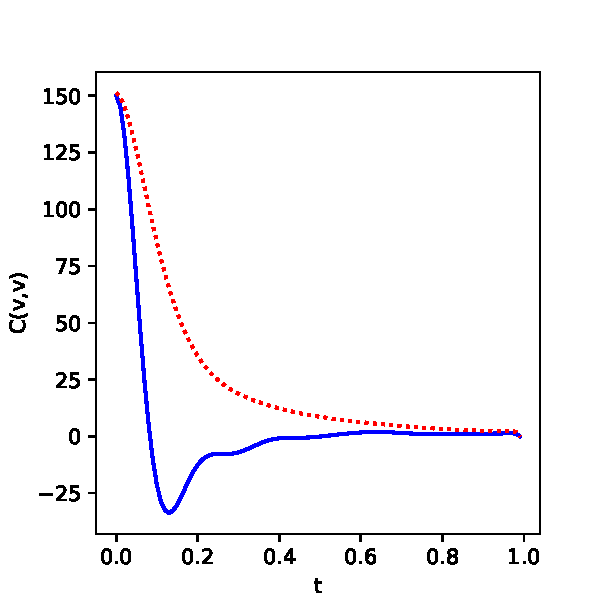
\includegraphics[width=0.5\textwidth]{plots/v_ac}
  \caption{Geschwindigkeitsautokorrelationsfunktion einer temperierten
    Lennard-Jones-Flüs\-sig\-ke\-it mit niedriger Dichte (rot
    gepunktet) und hoher Dichte (blau durchgezogen). Für die niedrige
    Dichte ist die Autokorrelationsfunktion im wesentlichen
    exponentiell abfallend, mit einer Korrelationszeit $\tau_c=0.17$,
    die durch die Kopplungszeit des Thermostaten bestimmt ist.}
  \label{fig:vac}
\end{figure}

\subsection{Autokorrelationsfunktion}

Im Spezialfall $A=B$ spricht man von der
\emph{\keyword{Autokorrelationsfunktion}}. Diese ist offenbar
symmetrisch, daher sind nur Zeitversätze $\tau\ge 0$ von
Interesse. Die Autokorrelationsfunktion misst gewissermaßen, wie lange
es dauert, bis die Observable nicht mehr von ihrem vorherigen Wert
abhängt, wann es diesen sozusagen "`vergisst"'. In dem häufigen Fall,
dass die Autokorrelationsfunktion zunächst exponentiell abfällt, lässt
sich dem Gedächtnis eine Zeitkonstante $\tau_c$, die
\emph{\keyword{Korrelationszeit}}, zuordnen. Diese kann man entweder
durch einen geeigneten Funktionsfit bestimmen, oder aber durch
Integration aus
\begin{equation}
  \label{eq:tauc}
  \int_{0}^{\infty} C(A,A)(\tau)\,d\tau = \int_{0}^{\infty}
  C(A,A)(0)e^{-\tau/\tau_c}\,d\tau = \tau_c\,C(A,A)(0).
\end{equation}

Abbildung~\ref{fig:vac} zeigt die Geschwindigkeitsautokorrelation
$C(v,v)$ einer temperierten Lennard-Jones-Flüs\-sig\-ke\-it bei zwei
verschiedenen Dichten. Die Temperierung wird dabei mit Hilfe eines
Thermostaten erreicht, der die Teilchen stochastisch an ein Wärmebad
koppelt. Dadurch dekorreliert die Geschwindigkeit eines Teilchens in
einer Korrelationszeit von etwa $1/6$.

$C(v,v)$ wird häufig dazu benutzt, um die Diffusionskonstante $D =
\int_0^{\infty} C(v,v)(\tau)\, d\tau$ des Systems zu bestimmen, die
also eng mit der Korrelationszeit des Thermostaten verwandt ist.  Bei
niedriger Dichte ist das System annähernd ein ideales Gas, und die
Teilchen dekorrelieren im wesentlichen nur durch den Einfluss des
Thermostaten, der durch Zufallskräfte wirkt, daher ist $C(v,v)$
tatsächlich gut exponentiell abfallend.  Formel~\eqref{eq:tauc}
bestimmt die Korrelationszeit mit guter Genauigkeit zu etwa
$\tau_c=0.17$, wie durch den Thermostaten zu erwarten. Im Falle der
dichteren Flüssigkeit hingegen kann diese Formel nicht angewendet
werden, da die Autokorrelation kein einfacher exponentieller Abfall
mehr ist, da auch Stoßprozesse eine wichtige Rolle spielen. Diese
führen zum Durchschwingen der Autokorrelationsfunktion.

\section{Messfehlerabschätzung}
\index{Messfehler}

In diesem letzten Abschnitt zur Datenanalyse geht es darum, wie der
Messfehler bei der Messung des Erwartungswerts einer stochastischen
Observable abgeschätzt werden kann. Wir betrachten also eine Messreihe
$x_i$, $i=1(1)N$, die verschiedene Messungen einer stochastischen
Observablen $x$ darstellen, deren Verteilung zeitlich unveränderlich
sein soll (wie zum Beispiel die Temperatur eines abgeschlossenen
Systems im Gleichgewicht). Die gesuchte Größe ist dann meist der
Erwartungswert $\mean{x}$ der Observablen oder ihre \emph{Varianz}
\begin{equation}
  \sigma^2(x) = \mean{\bigl(x-\mean{x}\bigr)^2}
  = \mean{x^2} - 2\mean{\mean{x}x}  + \mean{x}^2
  = \mean{x^2} - \mean{x}^2,
\end{equation}
die die erwartete quadratische Abweichung einer Messung vom
Erwartungswert beschreibt. Sie ist wie der Erwartungswert eine
Eigenschaft der zu messenden Observablen $x$ und im Gegensatz zum
Messfehler nicht von der Anzahl der Messungen abhängig.

Aus der Messreihe lässt sich der Erwartungswert dieser Observablen als
\begin{equation}
  \label{eq:mean}
  \mean{x} \approx \bar{x} := \frac{1}{N}\sum_{i=1}^N x_i
\end{equation}
abschätzen, da $\mean{\bar{x}} = \mean{x}$. Doch was ist nun der
Fehler, den wir mit dieser Schätzung machen? Dieser ist die zu
erwartende quadratische Abweichung des numerischen Mittelwerts vom
tatsächlichen Erwartungswert:
\begin{equation}
  \mean{\left(\overline{x} - \mean{x}\right)^2} =
  \frac{1}{N^2}\sum_{i,j=1}^N \mean{x_ix_j} -
  \frac{2}{N}\sum_{i=1}^N \mean{x_i}\mean{x} + \mean{x}^2
  = \frac{2}{N^2}\sum_{i > j} \mean{x_ix_j}
  + \frac{1}{N}\mean{x^2} - \mean{x}^2.
\end{equation}
An dieser Stelle nimmt man nun an, dass die Messungen paarweise
unabhängig sind, also, dass $\mean{x_ix_j} = \mean{x_i}\mean{x_j}$ für
$i\neq j$. In der Praxis lässt sich das zum Beispiel durch Betrachten
der Autokorrelationsfunktion sicherstellen, indem nur Messwerte mit
einem zeitlichen Abstand berücksichtigt werden, der sehr viel größer
als die Korrelationszeit ist. Diese Einschränkung werden wir im
folgenden noch genauer untersuchen, für den Moment nehmen wir die
Unabhängigkeit an und erhalten
\begin{equation}
  \label{eq:errestvar}
  \mean{(\overline{x} - \mean{x})^2}
  = \frac{N(N-1)}{N^2}\mean{x}^2 + \frac{1}{N}\mean{x^2} - \mean{x}^2
  = \frac{1}{N}\left(\mean{x^2} - \mean{x}^2\right)
  = \frac{1}{N}\sigma^2(x).
\end{equation}

Als Fehlerbalken wird üblicherweise die \emph{Standardabweichung} der
Messung $\overline{x}$ angegeben. Diese ist durch
\begin{equation}
  \sqrt{\mean{(\overline{x} - \mean{x})^2}}
  = \frac{1}{\sqrt{N}}\sigma(x)
\end{equation}
gegeben. Dies bedeutet, dass für eine Halbierung des Fehlerbalken
bereits viermal soviele Messungen durchgeführt werden müssen, und für
eine Größenordnung an Genauigkeit hundert Mal soviele. Besonders für
Computersimulationen ist das ein Problem, da die Rechenzeit im
allgemeinen proportional zur Anzahl der Messungen ist. Dauert also
eine Simulation eine Woche, was nicht ungewöhnlich ist, so würde eine
Messung mit einer Größenordnung mehr Genauigkeit fast zwei Jahre in
Anspruch nehmen!

Zur Berechnung des Fehlers benötigen wir noch eine Schätzung der
Varianz, die im Allgemeinen ebensowenig wie der Erwartungswert bekannt
ist und geschätzt werden muss. Dazu ersetzt man die Erwartungswerte in
$\mean{x^2} - \mean{x}^2$ durch den Schätzer \eqref{eq:mean}. Für
diesen Ausdruck gilt:
\begin{equation}
  \label{eq:varestalmost}
  \mean{\overline{x^2} - \bar{x}^2}
  = \mean{x^2} - 
  \frac{1}{N^2}\sum_{i=1}^n \mean{x_i^2}
  - \frac{1}{N^2}\sum_{i\neq j} \mean{x_ix_j}
  = \frac{N-1}{N}\left(\mean{x^2} - \mean{x}^2\right),
\end{equation}
wobei wir wieder annehmen, dass die Messungen unabhängig voneinander
sind. Der Ausdruck auf der linken Seite ist selber also \emph{kein} guter
Schätzer für die Varianz, obwohl er genau wie der Schätzer für den
Erwartungswert konstruiert ist. Das liegt daran, dass für die Schätzung
von $\mean{x}$ zweimal $\bar{x}$ und damit zweimal derselbe
Datensatz benutzt wurde.

Ein guter Schätzer für $\sigma^2(x)$ ergibt sich aus der Umkehrung von
\eqref{eq:varestalmost}:
\begin{equation}
  \label{eq:varest}
  \sigma^2(x) \approx \frac{N}{N-1}\left(\overline{x^2} -
    \bar{x}^2\right)
  = \frac{N}{N-1}\left(\overline{(x -
      \bar{x})^2}\right).
\end{equation}
Damit kann für unkorrelierte Daten der quadratische Fehler durch
\begin{equation}
  \label{eq:esterr}
  \mean{(\overline{x} - \mean{x})^2}
  \approx \frac{1}{N}\sigma^2(x)
  = \frac{1}{N-1}\left(\overline{x^2} - \bar{x}^2\right)
\end{equation}
abgeschätzt werden.

Auf dem Computer lassen sich $\mean{x}$ und $\sigma^2(x)$ mit Hilfe
von \eqref{eq:varest} bequem in einem Durchlauf der Daten abschätzen:
\begin{lstlisting}
sum  = 0
sum2 = 0
for v in x:
    sum  += v
    sum2 += v*v
mittel = sum/len(x)
sigma2 = (sum2/len(x) - mittel**2)*len(x)/(len(x)-1)
fehler = sqrt(sigma2/N)
\end{lstlisting}
Der zweite Weg in \eqref{eq:varest} via $\overline{(x - \bar{x})^2}$
ist zwar numerisch etwas stabiler, aber erfordert zwei Schleifen über
alle Daten, da der Mittelwert zunächst bestimmt werden muss, was unter
Umständen zu einer Verdoppelung der Laufzeit führen kann.

Selbstverständlich sind diese elementaren Schätzer aber auch direkt in
NumPy implementiert. \scipy{numpy.mean(x)} berechnet den Schätzer für
den Erwartungswert eines Arrays \argd{x}, \scipy{numpy.var(x, ddof=1)}
den Schätzer für seine Varianz. \argd{ddof} bezeichnet dabei die
Anzahl der abhängigen Freiheitsgrade, die von $N$ im Nenner von
\eqref{eq:varest} abgezogen werden. Wie wir eben gesehen haben, ist
dies bei unabhängigen Daten $\text{\argd{ddof}} = 1$.

\subsection{Fehler bei der Messung korrelierter Daten}

In der Praxis wird oft einfach angenommen, dass die Messungen
unabhängig sind. Was passiert nun, wenn dies nicht der Fall ist?
Betrachten wir also eine Observable die o.B.d.A. Erwartungswert
$\mean{x} = 0$ habe. Dann ist wie oben gezeigt
\begin{equation}
  \label{eq:correrr}
  \mean{(\overline{x} - \mean{x})^2} = \frac{2}{N^2}\sum_{i > j}
  \mean{x_ix_j}
  + \frac{1}{N}\sigma^2(x)
  = \frac{2}{N^2}\sum_{j=1}^{N}\sum_{n = 1}^{N-j} \mean{x_jx_{j+n}}
  + \frac{1}{N}\sigma^2(x).
\end{equation}
Für eine Observable $x$, die in gleichmäßigen Zeitabständen $\Delta$
gemessen wird, lässt sich die innere Summe des linken Terms mit Hilfe
der Autokorrelationsfunktion $C(\tau) = C(x,x)(\tau)$
abschätzen:\nobreak
\begin{equation}
  \sum_{n = 1}^{N-j} \mean{x_jx_{j+n}}
  \approx \int_{n = 0}^{\infty} C(n\Delta)
  = \frac{\tau_c}{\Delta} C(0)
  = \frac{\tau_c}{\Delta}\sigma^2(x),
\end{equation}
wobei $\tau_c$ die Korrelationszeit gemäß \eqref{eq:tauc} ist und
entsprechend ein einfacher exponentieller Abfall angenommen
wurde. Außerdem muss $\tau_c\ll N\Delta$ sein, so dass die Erweiterung
des Integrals bis unendlich keinen nennenswerten Beitrag mehr
liefert. Eingesetzt in \eqref{eq:correrr} ergibt sich
\begin{equation}
  \label{eq:correrrest}
  \mean{(\overline{x} - \mean{x})^2}
  \approx
  \frac{2}{N^2}\sum_{j=1}^{N} \frac{\tau_c}{\Delta}\sigma^2(x)
  + \frac{1}{N}\sigma^2(x)
  =
  \left(1 + 2\frac{\tau_c}{\Delta}\right)\frac{\sigma^2(x)}{N}.
\end{equation}
Der Fehler ist also um einen Faktor $1 + 2 \tau_c /\Delta$
\emph{größer}, als man aufgrund der Varianz und Anzahl Messungen
erwarten würde, wenn man einfach annimmt, dass die Messungen
unabhängig sind. Setzt man $N_\text{eff} = N \Delta / (2\tau_c)$, dann
ergibt sich
\begin{equation}
  \label{eq:errestvarcorr}
  \mean{(\overline{x} - \mean{x})^2}
  \approx
  \left(1 + 2\frac{\tau_c}{\Delta}\right)\frac{\sigma^2(x)}{N}.
  \approx \frac{\sigma^2(x)}{N_\text{eff}}.
\end{equation}
Mit anderen Worten, $N_\text{eff}$ kann als die Anzahl der tatsächlich
unabhängigen Messungen interpretiert werden. Nur Messungen, die etwa
zwei Autokorrelationszeiten auseinanderliegen, sind hinreichend
unabhängig.

Auch der Schätzer \eqref{eq:varest} für die Varianz setzt die
Unabhängigkeit der Messungen voraus. Für abhängige Daten ergibt sich
\begin{align}
  \frac{N}{N-1}\mean{\overline{x^2} - \bar{x}^2}
  &= \frac{1}{N-1}\left(N\mean{x^2} - \mean{x^2}
    - \frac{1}{N}\sum_{i\neq j} \mean{x_ix_j}\right)\nonumber\\
  &= \sigma^2(x) - \frac{2}{N(N-1)}\sum_{i> j} \mean{x_ix_j}
  \approx \left(1 - 2\frac{\tau_c}{\Delta N}\right)\sigma^2(x).
\end{align}
Die Varianz wird also zusätzlich um einen Faktor $1 -
2\frac{\tau_c}{\Delta N}$ \emph{unterschätzt}. Immerhin lässt sich
dieser Fehler durch ausreichend viele Messungen minimieren. Allerdings
bringt es nichts, einfach häufiger zu messen, sondern man muss
tatsächlich länger messen, da ja die Gesamtmesszeit $\Delta N$
eingeht.

\begin{figure}
  \centering
  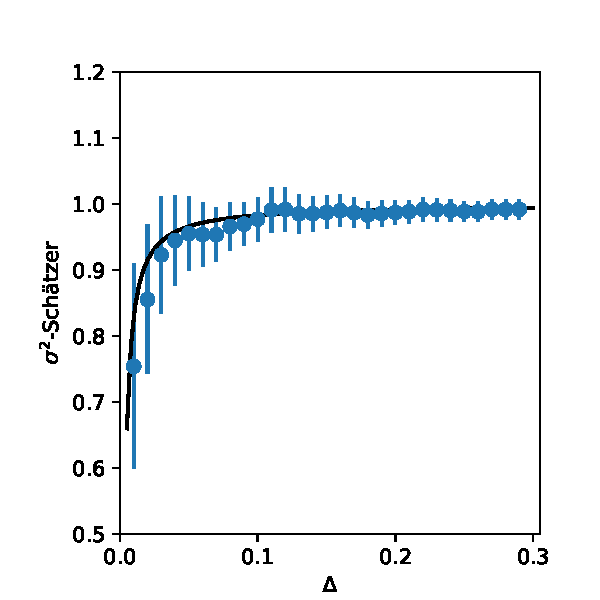
\includegraphics[width=0.5\textwidth]{plots/error}
  \caption{Geschätzte, scheinbare Varianz der Komponenten der
    Geschwindigkeitsverteilung in einem dünnen temperierten
    Lennard-Jones-Systems als Funktion der gewählten Schrittweite
    $\Delta$. Analytisch erwartet man bei der gewählten Temperatur
    eine Varianz von 1. Die blauen Balken geben das
    $1\sigma$-Intervall der beobachteten Varianzen an. Die schwarze
    Linie zeigt die Abschätzung der scheinbaren Varianz gemäß
    \eqref{eq:correrrest} als $(1-2\tau_c/(\Delta N))\sigma^2(x)$, was
    gut zu den gemessenen Daten passt.}
  \label{fig:error}
\end{figure}

Abbildung~\ref{fig:error} zeigt die scheinbare Varianz der Verteilung
der einzelnen Komponenten der Geschwindigkeit als Funktion der
gewählten Messschrittweite im weniger dichten thermalisierten
Lennard-Jones-System. Diese Geschwindigkeiten sind im thermischen
Gleichgewicht normalverteilt um die Null mit einer Varianz
proportional zur Temperatur des Systems. Im Falle der hier benutzten
Simulationen stellt ein Thermostat sicher, dass die Temperatur exakt 1
ist. Wie man in Abbildung~\ref{fig:error} allerdings deutlich sieht,
wird mit korrelierten Messungen die Varianz, und damit die Temperatur,
um bis zu 25\% unterschätzt, sofern zwischen den Messungen deutlich
weniger Zeit als die Korrelationszeit des Systems, $\approx 0,17$,
liegt. Im Beispiel wurden alle $0,01$ Schritte insgesamt 50.000 Daten
erhoben. Der quadratische Fehler der beobachteten mittleren
Geschwindigkeitskomponenten ist also $1\cdot 34/50.000 \approx 7\cdot
10^{-4}$ anstatt $2\cdot 10^{-5}$, wie man ohne Berücksichtigung der
Korrelationen erhalten würde.

Im Falle der Temperatur gibt es eine einfache Abhilfe, da die
Temperatur auch aus der kinetische Energie abgeschätzt werden kann,
allerdings ist das nicht immer der Fall. So wird die Wärmekapazität
eines Systems aus der Varianz der Energiedichte bestimmt, und die
dielektrische Konstante aus der Varianz des Dipolmoments. In diesem
Fall ist es also enorm wichtig, mit ausreichend vielen unkorrelierten
Daten zu arbeiten.

\subsection{Binning-Analyse}
\index{Binning}

Im obigen Beispiel ist die Autokorrelationsfunktion tatsächlich
einfach exponentiell und daher die Autokorrelationszeit einfach zu
bestimmen. Bei den meisten komplexen Systemen ist das nicht der Fall.
Trotzdem lässt sich \eqref{eq:correrrest} anwenden, allerdings geht
dann die \emph{integrierte} Autokorrelationszeit
\begin{equation}
  \tau_\text{int} := \frac{1}{C(A,A)(0)}\int_0^\infty C(A,A)(\tau)\,d\tau
\end{equation}
ein. Eine Möglichkeit, diese abzuschätzen, ist die
Binning-Analyse~\cite{janke02a}. Diese Methode liefert direkt den
Messfehler, kann aber auch benutzt werden, um die $\tau_\text{int}$ zu
bestimmen.

Dazu seien die Daten $x$ in $B$ Blöcke (\enquote{Bins}) der Länge $k$
eingeteilt. Ist $N$ nicht durch $k$ teilbar, muss dazu der Datensatz
etwas gekürzt werden, so dass alle Blöcke voll sind. Anstatt der
einzelnen Daten in den Blöcken, betrachten wir nun nur ihre jeweiligen
Mittelwerte
\begin{equation}
  X_{k,l} = \frac{1}{k}\sum_{j=1}^{k}x_{(l-1)k + j}\quad l=1(1)B.
\end{equation}
Offenbar hängen der Erwartungswert und die Varianz der einzelnen
$X_{k,l}$ nicht vom Aufpunkt $l$ ab. Wir schreiben daher kurz $X_k$
für die Observable der Blockmittelwerte der Länge $k$.  Der
Erwartungswert von $X_k$ ist unverändert der von $x$, also $\mean{X_k}
= \mean{x}$, und auch für den Mittelwert aller $X_k$ gilt $\bar{X} =
\bar{x}$. Allerdings ist die Varianz $\sigma^2(X_{k})$ im allgemeinen
von $\sigma^2(x)$ verschieden, und zwar abhängig von $k$. Sofern $k$
sehr viel größer als die typischen Korrelationslängen ist, gilt nach
\eqref{eq:errestvarcorr} $\sigma^2(X_{k}) \approx
\sigma^2(x)/k_\text{eff}$, wobei $k_\text{eff} = k \Delta /
(2\tau_\text{int})$ die effektive Anzahl der unabhängigen Messungen
ist. Für sehr kleine $k$ hingegen spielt die Mittelung keine Rolle,
daher ist $\sigma^2(X_{k}) \approx \sigma^2(x)$.

Diese Verhalten nutzen wir nun, um den Fehler korrelierter Daten
abzuschätzen. Dazu berechnen wir den quadratischen Fehlerschätzer
\eqref{eq:esterr} für die Blockmittelwerte bei verschiedenen
Blockgrößen $k$:
\begin{equation}
  \epsilon^2(k) := \frac{1}{B - 1} \left(\overline{X_k^2} -
    \overline{X_k}^2\right) \approx \frac{k}{N} \sigma^2(X_k).
\end{equation}
Ist $k$ klein, so ist $\sigma^2(X_k)\approx \sigma^2(x)$, und
$\epsilon^2(k)$ wächst linear in $k$. Für große $k$ hingegen ist
$\sigma^2(X_k) \approx \sigma^2(x)/k_\text{eff}$, so dass
$\epsilon^2(k)$ konstant wird, und zwar
\begin{equation}
  \epsilon^2(k)= \frac{k}{N}\frac{\sigma^2(x)}{k_\text{eff}} =
  \frac{\sigma^2(x)}{N_\text{eff}}.
\end{equation}
Der konstante Wert bei großen $k$ ist also der gesuchte tatsächliche
Fehler!  Allerdings stehen bei großen $k$ für die Mittelung immer
weniger Blöcke zur Verfügung, so dass $\epsilon^2(k)$ stark
verrauscht. Daher funktioniert diese Analyse nur, sofern man genügend
Daten gesammelt hat. Auch die Umkehrung gilt: trägt man
$\epsilon^2(k)$ gegen $k$ auf und sieht kein Plateau bei großen $k$,
hat man noch nicht genügend Daten gesammelt, um eine Aussage über die
Güte der Messung zu machen, man benötigt also mehr Daten.

Neben des Fehlers lässt sich für große $k$ auch die integrierte
Autokorrelationszeit gemäß
\begin{equation}
  \label{eq:tauint}
  k \Delta\frac{\sigma^2(X_k)}{\sigma^2(x)} \approx
  \frac{k\Delta}{k_\text{eff}} = 2\tau_\text{int}
\end{equation}
bestimmen, wobei die Messung von $\sigma^2(x)$ ausreichend unabhängige
Daten voraussetzt. Dies überprüft man zunächst anhand von
$\epsilon^2(k)$.

\begin{figure}
  \centering
  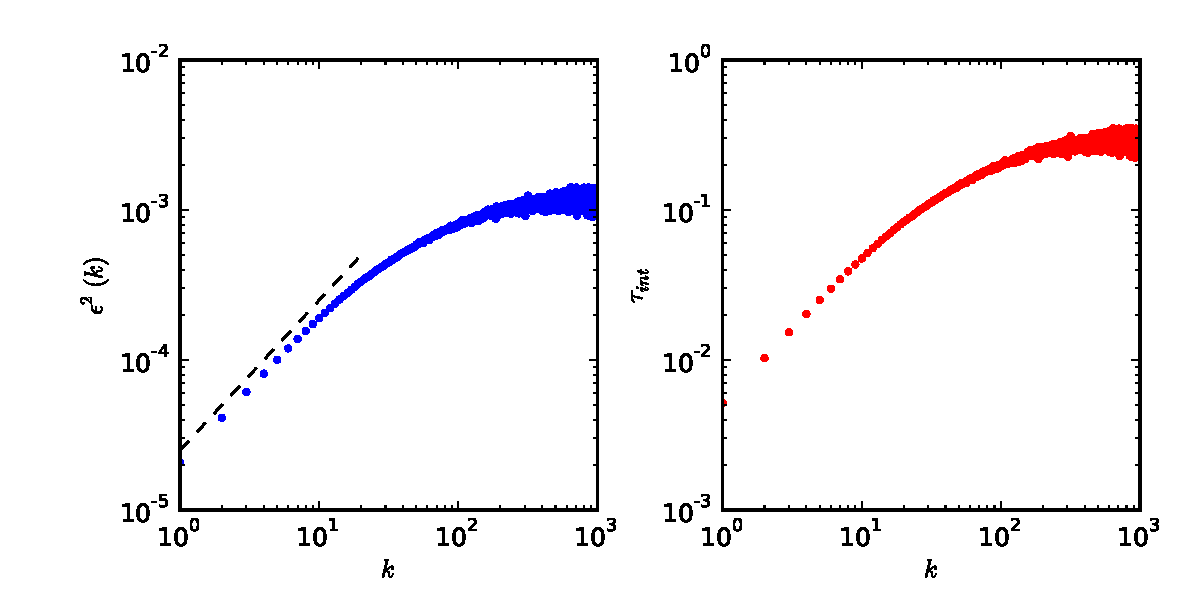
\includegraphics[width=\textwidth]{plots/binning}
  \caption{Links: geschätzter quadratischer Fehler $\epsilon^2(k)$ in
    der Messung der Komponenten der Geschwindigkeitsverteilung in
    einem dünnen temperierten Lennard-Jones-Systems als Funktion der
    Blockgröße $k$. Der Fehler erreicht sein Plateau bei etwa
    0,001, was gut mit der Abschätzung über die Autokorrelationszeit
    übereinstimmt.  Die gestrichelte schwarze Linie demonstriert das
    lineare Wachstum für kleine $k$. Rechts: Geschätzte integrierte
    Autokorrelationszeit $\tau_\text{int}$ für dasselbe System.  Diese
    erreicht ihr Plateau bei $\tau_\text{int} \approx 0,25$, was etwas
    größer als $\tau_c$ ist.}
  \label{fig:binning}
\end{figure}

Abbildung~\ref{fig:binning} demonstriert die Abschätzung des
quadratischen Fehlers und der integrierten Autokorrelationszeit für
die Messung der Geschwindigkeitskomponenten in der
Lennard-Jones-Flüssigkeit. Wie erwartet werden beide Größen für große
$k$ konstant, aber sind verrauscht, während sie für kleine $k$ linear
anwachsen.  Für die Bestimmung der integrierten Autokorrelationszeit
wurde das analytische Ergebnis $\sigma^2(x)=1$ benutzt, die gemessene
ist mit $1,03$ etwas größer. Aus der Binning-Analyse ergibt sich ein
quadratischer Fehler von etwa 0,001 und eine integrierte
Autokorrelationszeit von 0,25, was gut zu unserer Autokorrelationszeit
$0,17$ und der Fehlerschätzung von $7\cdot 10^{-4}$ passt.

\section{Ausgleichsrechnung, Methode der kleinsten Quadrate}
\index{Ausgleichsrechnung}
\index{Fitting}
\index{Methode der kleinsten Quadrate}

\begin{figure}
  \centering
  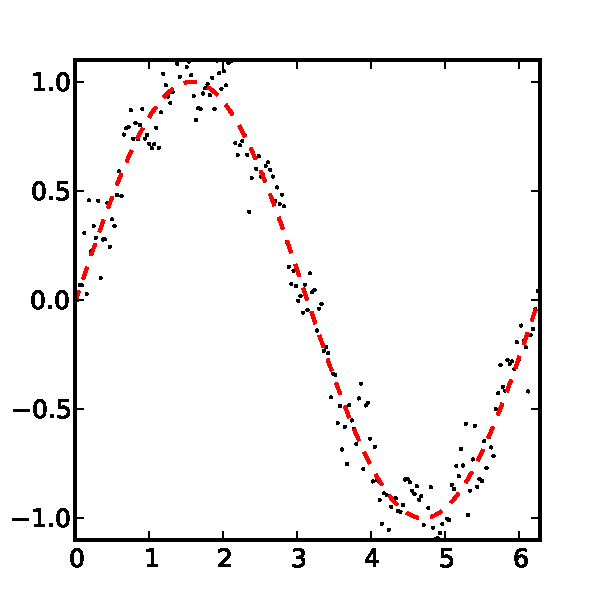
\includegraphics[width=0.5\textwidth]{plots/leastsq}
  \caption{Methode der kleinsten Quadrate zum Fitten der Sinusfunktion
    $y=\sin(x)$. 200 Datenpunkte zwischen 0 und $2\pi$ wurden als
    $\sin(x) + 0,1\,\sin(10 x) + \xi$ erzeugt, wobei $\xi$ eine
    Gauß-verteilte Pseudozufallsvariable mit Varianz $0,01$ war. Die
    resultierende Sinusfunktion (rot gestrichelt) hat die Form $a
    \sin(bx+c)$, wobei die Koeffizienten auf gut 2\% Genauigkeit
    $a=b=1$ und $c=0$ entsprechen. Die kleine höherfrequente
    Schwingung kann durch einen Fit allerdings nicht zuverlässig
    erkannt werden, anders als durch eine Fouriertransformation,
    vergleiche Abbildung~\ref{fig:fourieralias}}
  \label{fig:leastsq}
\end{figure}

Interpolierende Polynome, Taylorreihen und Splines haben gemeinsam,
das diese möglichst nahe an alle gegebenen Stützstellen verlaufen. Die
Anzahl der Terme in der Approximation ist nur durch die Anzahl der
Stützstellen begrenzt, und meist wählt man so viele Stützstellen wie
möglich, um eine möglichst genaue Näherung der unbekannten
Funktionsform zu erhalten.

Wenn die Daten an den Stützstellen aus Experimenten oder
Computersimulationen gewonnen werden, ist das aber gar nicht
gewünscht, da die Daten selbst nicht exakt sind. Wie wir gesehen
haben, kann deren Qualität zwar durch Mittelung verbessert werden,
trotzdem bleibt eine gewisse Unsicherheit.  Andererseits hat man in
diesem Fall üblicherweise eine Vorstellung aus der Theorie, welche
funktionelle Form die Daten annehmen, und möchte nun wissen, bei
welcher Parameterwahl diese Funktion am besten mit den Daten
verträglich ist. Man möchte also den Parametersatz bestimmen, der den
Abstand der Daten von der Funktion minimiert. Dabei ist bei sinnvollen
Experimenten die Anzahl der Datenpunkte sehr viel größer als die
Anzahl der Parameter.

Seien also wieder Daten $(x_i, y_i)$, $i=0(1)n-1$ und eine Funktion
$f_v(x)$ gegeben. Gesucht ist dann derjenige Parametervektor $v$, der
die Abweichung
\begin{equation}
  \label{eq:leastsq}
  \Delta(v) = \sum_i (f_v(x_i) - y_i)^2
\end{equation}
minimiert. Dieses Verfahren wird auch Methode der kleinste Quadrate
genannt, da ja die quadrierten Abweichungen minimiert werden
sollen. Ist $f_{a,b}(x) = ax + b$ eine Gerade, spricht man auch von
\emph{linearer Regression}\index{lineare Regression}. In diesem Fall lässt
sich das Optimum einfach bestimmen, da
\begin{equation}
  0 = \frac{d}{da} \Delta(a,b) = \sum_i 2 (a x_i + b - y_i)x_i
  = 2n \left(a  \overline{x_i^2} + b \overline{x_i} -
    \overline{y_ix_i} \right)
\end{equation}
und
\begin{equation}
  0 = \frac{d}{db} \Delta(a,b) = \sum_i 2 (a x_i + b - y_i)
  = 2n \left(a  \overline{x_i} + b - \overline{y_i} \right),
\end{equation}
wobei $\overline{x} = \frac{1}{n} \sum_{i=0}^{n-1} x_i$ den Mittelwert
über alle Datenpunkte bedeutet. Daraus ergibt sich
\begin{equation}
  a = \frac{\overline{y_ix_i} -
    \overline{y_i}\cdot\overline{x_i}}{\overline{x_i^2}-\overline{x_i}^2}
  \quad\text{und}\;
  b = \overline{y_i} - a \overline{x_i},
\end{equation}
was sich einfach auf dem Computer berechnen lässt.

Auch für quadratische und andere einfache Funktionen lassen sich die
Koeffizienten geschlossen darstellen, aber bei allgemeinen Funktionen
ist dies nicht immer der Fall. Dann muss die nichtlineare
Optimierungsaufgabe \eqref{eq:leastsq} numerisch gelöst werden, was
wir später behandeln werden. Für den Moment genügt uns, dass SciPy die
Funktion \scipy{scipy.optimize.leastsq(delta, v0, (x, y))} dafür
bereitstellt. \argd{(x, y)} sind dabei die Ausgangsdaten, die hier zu
einem Tupel zusammengefasst sind. \argd{v0} ist der Startwert für die
Berechnung, der nicht zu weit vom (unbekannten) Optimum entfernt
liegen darf. \argd{delta} ist eine Python-Funktion, die als Argumente
$v$, $x_i$ und $y_i$ nimmt und $f_v(x_i) - y_i$ zurückliefert.  Da
$f_v(x)$ eine beliebig komplizierte Form annehmen kann, ist diese
Aufgaben im Allgemeinen nicht lösbar, allerdings funktioniert ein
solcher \emph{Fit} für einfache Funktionen meistens recht
gut. Abbildung~\ref{fig:leastsq} zeigt einen solchen Funktionsfit an
eine verrauschte Sinusfunktion, die mit 200 Datenpunkten auf etwa 2\%
genau gefittet werden kann. Man beachte, das der Ausgangswert für den
Fit mit Hilfe der SciPy-Funktion \lstinline!leastsq! $a=0$, $b=1$,
$c=0$ war; beim Startwert $a=0$, $b=0$, $c=0$ bricht das Verfahren
ab. Das zeigt, dass man tatsächlich nicht zu weit vom Optimum starten
kann, was ein gewisses Verständnis der Zielfunktion voraussetzt.

Ist die Funktionsform, die den Daten zugrundeliegt, unbekannt, ist es
normalerweise keine gute Idee, die Form zu raten. Generell sollte auch
die Anzahl der Parameter sehr klein sein, da sich sonst fast alles
"`gut"' fitten lässt ("`With four parameters I can fit an elephant and
with five I can make him wiggle his trunk."' --- J. von Neumann).

Soll aber zum Beispiel für Visualisierungszwecke eine ansprechende
Kurve entlang der Daten gelegt werden, deren tatsächliche Abhängigkeit
unbekannt ist, dann sind \emph{Pad\'e-Funktionen} oft eine gute
Wahl. Diese haben die Gestalt $P(x)/Q(x)$, wobei $P$ und $Q$ zwei
Polynome mit paarweise verschiedenen Nullstellen sind. Üblicherweise
lassen sich schon für niedrige Polynomgrade ansprechende Fits finden,
sofern die Grade der beiden Polynome in etwa gleich gewählt werden.

%%% Local Variables: 
%%% mode: latex
%%% TeX-master: "padc"
%%% TeX-PDF-mode: t
%%% End: 

% Dies ist Teil der Vorlesung Physik auf dem Computer, SS 2012,
% Axel Arnold, Universitaet Stuttgart.
% 
% Dieses Werk ist unter einer Creative Commons-Lizenz vom Typ
% Namensnennung-Weitergabe unter gleichen Bedingungen 3.0 Deutschland
% zugänglich. Um eine Kopie dieser Lizenz einzusehen, konsultieren Sie
% http://creativecommons.org/licenses/by-sa/3.0/de/ oder wenden Sie sich
% schriftlich an Creative Commons, 444 Castro Street, Suite 900, Mountain
% View, California, 94041, USA.

\chapter{Nichtlineare Gleichungssysteme}
\index{Nullstellensuche}
\index{Fixpunktsuche}

Im zweiten Kapitel hatten wir uns mit der Lösung linearer
Gleichungssysteme beschäftigt, die ja eine wesentliche Grundlage der
numerischen Mathematik darstellen. Allerdings tauchen in der Praxis,
besonders in der Physik, leicht auch nichtlineare Gleichungssysteme
auf. In diesem Fall kann man meist keine allgemeine Aussage über
Existenz und Anzahl der Lösungen machen und auch keine exakten
Verfahren zur Lösung angeben.

Nichtlineare Gleichungssysteme werden typischerweise in zwei Formen
betrachtet. Sei eine Funktion $f:M\subseteq\RR^n\to\RR^n$ gegeben. Dann suchen
wir die \emph{Nullstellen}
\begin{equation}
  \label{eq:nullstellen}
  x, \quad\text{so dass}\; f(x) = 0,
\end{equation}
also die Lösungen zur Gleichung $f(x) = 0$. Man beachte, dass anders
als im Fall der linearen Gleichungssysteme gefordert wird, dass der
Bildraum wie auch der Ursprungsraum $M$ zu einem Vektorraum derselben
Dimension $n$ gehören. Ohne diese Voraussetzung ist eine eindeutige
Lösung im Allgemeinen unmöglich. Anders als im Falle der linearen
Gleichungssysteme ist es hier auch nicht ohne Weiteres möglich, den
Lösungsraum anzugeben, falls die Lösung nicht eindeutig
ist. Tatsächlich kann der Lösungsraum ja eine beliebig komplexe
Mannigfaltigkeit innerhalb $M$ darstellen, die dann gar nicht
geschlossen parametrisiert werden kann. Das macht die numerische
Bestimmung dieser Lösungsmannigfaltigkeit sehr schwierig.

Alternativ können wir für eine Funktion $g:M\subseteq\RR^n\to\RR^n$ die
\emph{Fixpunkte} suchen. Diese sind
\begin{equation}
  \label{eq:fixpunkt}
  x, \quad\text{so dass}\; g(x) = x,
\end{equation}
also die Lösungen der Gleichung $g(x) = x$. Eine Fixpunktgleichung
lässt sich natürlich stets auch als Nullstellenproblem mit $f(x) =
g(x) - x$ formulieren und umgekehrt.

Die beiden Formulierungen unterscheiden sich allerdings im natürlichen
Lösungsansatz. Die Nullstellengleichung \eqref{eq:nullstellen} ähnelt
dem linearen Gleichungssystem \eqref{eq:lgs}. Das
\emph{Newtonverfahren} beruht auf einer lokalen Linearisierung und dem
Lösen dieses linearen Gleichungssystems. Die Fixpunktgleichung
hingegen legt nahe, den Fixpunkt durch \emph{sukzessive Substitution}
zu suchen: $x_0\to g(x_0)\to g(g(x_0))\to\ldots$.

\section{Sukzessive Substitution}
\index{sukzessive Substitution}
\index{Fixpunktsuche}

Eine Abbildung $g:M\to M$ mit $M\subset\RR^n$ heißt Lipschitz-stetig
(L-stetig), falls es ein $L\in\RR$ gibt, so dass
\begin{equation}
  \norm{g(x) - g(y)} \le L \norm{x - y}\quad\forall x,y\in M.
\end{equation}
Alle auf $M$ differenzierbaren Funktionen mit beschränkter Ableitung
sind L-stetig, wenn ihre Ableitung beschränkt ist. Die
Lipschitzkonstante ergibt sich aus dem Mittelwertsatz zu $L=\max_{x\in
  M}\norm{g'(x)}$.  Es gibt allerdings noch mehr L-stetige Funktionen,
zum Beispiel die in 0 nicht differenzierbare Betragsfunktion, die auf
ganz $\RR$ L-stetig mit $L = 1$ ist. Auf der anderen Seite ist
offenbar jede L-stetige Funktion auch stetig, \dh\,, die L-stetigen
Funktionen sind eine eigene Klasse zwischen den stetigen und
differenzierbaren Funktionen. Dabei ist es nicht wesentlich, welche
Norm $\norm{\cdot}$ genutzt wird. Sie kann für das Problem geeignet
gewählt werden, sofern sie die üblichen Bedingungen an eine Norm, wie
etwa die Dreiecksungleichung, erfüllt.

\index{Banachscher Fixpunktsatz} Hat eine Funktion $g:M\to M$ eine
Lipschitz-Konstante $L<1$, so heißt $g$ \emph{kontrahierend}, weil
zwei verschiedene Punkte durch die Abbildung stets näher aneinander
geschoben werden. Wir betrachten nun einen beliebigen Startpunkt
$x_0\in M$ und definieren damit die Folge der \emph{sukzessiven Substitution}:
\begin{equation}
  x_{n} := g(x_{n-1}) \quad\text{für}\; n\ge 1.
\end{equation}
Dann gilt für alle $n,m\in\NN$ der \emph{Banachsche Fixpunktsatz}
\begin{align}
  \label{eq:banach}
  \norm{x_{n+m} - x_n} \,=\, &\norm{\sum_{k=0}^{m-1} x_{n+k+1} - x_{n+k}}
  \,\le\, \sum_{k=0}^{m-1} \norm{x_{n+k+1} - x_{n+k}}\nonumber\\
  \,=\, &\norm{g(g(\ldots g(x_{n+1}))) - g(g(\ldots g(x_{n})))}
  + \cdots\nonumber\\
  &+ \norm{g(g(x_{n+1})) - g(g(x_{n}))}
  + \norm{g(x_{n+1}) - g(x_{n})} + \norm{x_{n+1} - x_{n}}\nonumber\\
  \le\, &\sum_{k=0}^{m-1} L^k \norm{x_{n+1} - x_{n}}
  \,\le\, \frac{1}{1-L}\norm{x_{n+1} - x_{n}} \le
  \frac{L^n}{1-L}\norm{g(x_0) - x_0}.
\end{align}
Die sukzessive Substitution definiert also eine Cauchyfolge, die in
$M$ konvergiert, sofern $M$ abgeschlossen ist (\zb $M=\RR^n$ oder $M$
Einheitskugel). Für den Grenzwert $\overline{x}$ dieser Folge gilt
\begin{equation}
  \overline{x} = \lim_{n\to\infty}x_{n+1} = \lim_{n\to\infty}g(x_{n})
  = g(\overline{x}),
\end{equation}
er ist also ein Fixpunkt.

Wir betrachten nun zwei Fixpunkte $\overline{x}$ und $\overline{y}$. Dann gilt
\begin{equation}
  \norm{\overline{x} - \overline{y}} = \norm{g(\overline{x}) -
    g(\overline{y})} \le L \norm{\overline{x} - \overline{y}} \implies
  \overline{x} = \overline{y}.
\end{equation}
Das bedeutet, dass es nur genau einen Fixpunkt $\overline{x}$ von $g$
in $M$ gibt, und dass die sukzessive Substitution für jeden Startwert
\emph{global} gegen $\overline{x}$ konvergiert. \eqref{eq:banach}
gibt auche eine \textit{a priori}-Abschätzung des Fehlers:
\begin{equation}
  \norm{\overline{x} - x_n} \le \frac{L^n}{1-L}\norm{g(x_0) - x_0}
\end{equation}
sowie eine Abschätzung der Konvergenzrate:
\begin{equation}
  \frac{\norm{x_{n+1} - \overline{x}}}{\norm{x_n - \overline{x}}}
  = \frac{\norm{g(x_n) - g(\overline{x})}}{\norm{x_n - \overline{x}}}
  \le L < 1.
\end{equation}
Die sukzessive Substitution konvergiert also linear. Das Verfahren
wird abgebrochen, wenn $\norm{x_{n+1} - x_n}$ hinreichend klein ist,
da dann nach \eqref{eq:banach} auch
\begin{equation}
  \norm{\overline{x} - x_n} \le \frac{1}{1-L}\norm{x_{n+1} - x_n}.
\end{equation}
Offenbar konvergiert die sukzessive Substitution um so schneller, je
kleiner die Lipschitzkonstante $L$ ist.

Neben der globalen Konvergenzeigenschaft konvergiert die sukzessive
Substituion auch lokal: ist $g:\RR^n\to\RR^n$ eine differenzierbare
Funktion und hat einen Fixpunkt $\overline{x}$ mit $\norm{g'(x)} < 1$,
so gibt es eine Umgebung des Fixpunktes, in dem die sukzessive
Substitution gegen diesen Fixpunkt konvergiert.

\begin{figure}
  \centering
  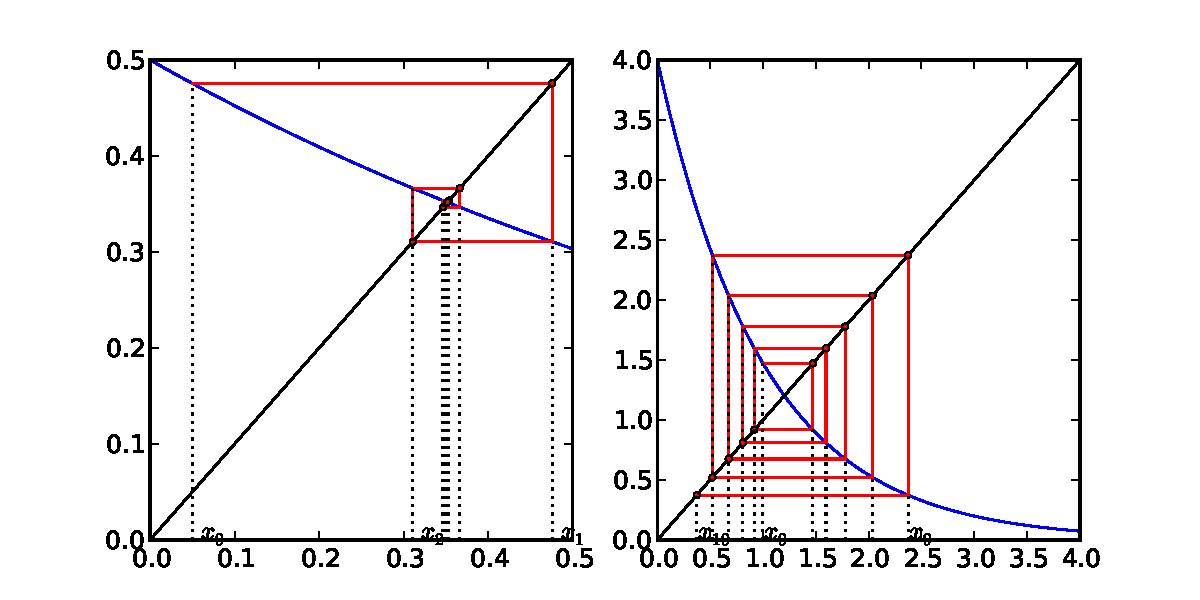
\includegraphics[width=\textwidth]{plots/banach}
  \caption{Sukzessive Substitution mit Funktion $g(r) = e^{-r}/\phi_0$
    mit $\phi_0=2$ (links) und $\phi_0=1/4$ (rechts). Blau
    durchgezogen ist die Funktion $g$, die Winkelhalbierende ist
    schwarz dargestellt. Die Punkte auf der Winkelhalbierenden
    markieren die Punkte $(x_1,x_1)$, $(x_2,x_2)$ \usw\,, durch die das
    Lot auf $g$ gefällt wird, um den nächsten Punkt der sukzessiven
    Substitution zu erhalten. Im linken Graph sind die ersten sieben
    Glieder dargestellt, die exponentielle Konvergenz ist gut zu
    sehen. Im rechten Graph konvergiert das Verfahren nicht mehr.}
  \label{fig:banach}
\end{figure}

\subsection{Beispiel}

Als Beispiel für eine Anwendung des Banachschen Fixpunktsatzes
betrachten wir die dimensionslose Form des Yukawa- oder
Debye-Hückel-Potentials $\phi(r) = e^{-r}/r$. Wir fragen uns, wann für
welches $r$ dieses Potential einen gegeben Wert $\phi_0$ annimmt. Das
führt zu der Fixpunktgleichung
\begin{equation}
  g(r) = \frac{e^{-r}}{\phi_0} = r
\end{equation}
Die linke Seite ist eine auf $[0,\infty)$ L-stetige Funktion mit
$L=1/\phi_0$, wie man durch Ableiten leicht sieht.

Abbildung~\ref{fig:banach} zeigt die sukzessive Substitution für
$g(r)$. Graphisch lässt sich das Verfahren visualisieren, indem in
jeder Iteration der Funktionswert $x_{n+1} = y =g(x_{n})$ an der
Winkelhalbierenden $y=x$ auf die $x$-Achse zurückgespiegelt wird. Im
linken Graph ist $\phi_0=2$ und damit $L=1/2$, so dass die sukzessive
Substitution exponentiell konvergiert. Für das letzte abgebildete
Glied, $x_7$, gilt $\abs{x_7-\overline{x}} \le 1/2^8 = 1/256$. Im
rechten Graph ist $\phi_0=1/4$ und damit $L=4$. Insbesondere ist auch
im Fixpunkt $g'(\overline(x))>1$. Abgebildet sind die ersten zehn
Glieder der sukzessiven Substitution, die hier nicht mehr
konvergiert. Wird hingegen $\phi_0$ so gewählt, dass 
$g'(\overline(x))<1$, aber $L>1$, so konvergiert das Verfahren zwar
noch, aber nicht mehr exponentiell.

\section{Newtonverfahren in einer Dimension}
\index{Newtonverfahren}
\index{Nullstellensuche}

Nachdem wir bis jetzt die sukzessive Substitution zur Bestimmung von
Fixpunkten betrachtet haben, geht es nun um die Nullstellensuche. Sei
also zunächst eine stetig differenzierbare Funktion $f:[a,b]\to\RR$
gegeben und deren Nullstellen $x$, $f(x) = 0$, gesucht. Ähnlich wie
bei der sukzessiven Iteration starten wir mit einem Startwert
$x_0$. Um uns nun der Nullstelle der Funktion zu nähern, linearisieren
wir in der aktuellen Näherung $x_n$ und lösen nach der Nullstelle
$x_{n+1}$ auf:
\begin{equation}
  x_{n+1} = g(x_n) := x_n - \frac{f(x_n)}{f'(x_n)}\quad\text{für}\; n\ge 0,
\end{equation}
wobei wir annehmen, dass $f'(x)\neq 0$ auf $[a,b]$.  Für eine
Nullstelle $\overline{x}$ von $f$ gilt offenbar $g(\overline{x}) =
\overline{x}$, \dh wir suchen einen Fixpunkt von $g$, den wir wieder
durch sukzessive Substitution annähern können. Man bricht das
Verfahren wie auch die sukzessive Substitution ab, wenn
$\abs{x_{n}-x_{n-1}}$ bzw. $\abs{f(x_n)}$ hinreichend klein sind.

\begin{figure}
  \centering
  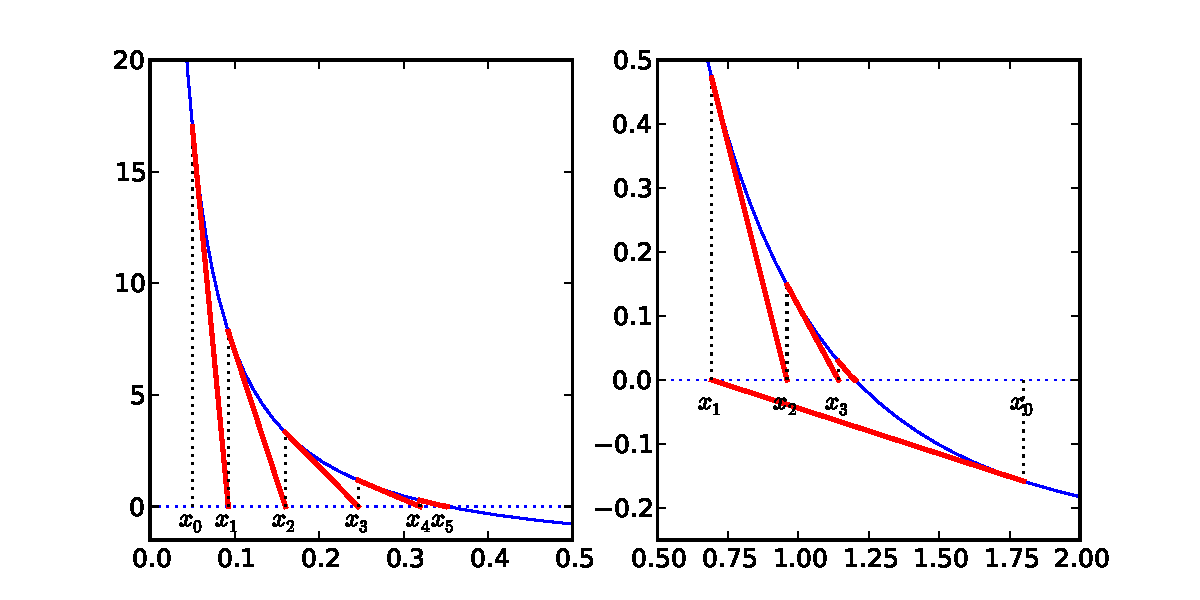
\includegraphics[width=\textwidth]{plots/newton}
  \caption{Newtonverfahren für die Funktion $f(r) = e^{-r}/r -
    \phi_0$. Wie schon beim Graphen zur sukzessiven Substitution ist
    links $\phi_0=2$, rechts $\phi_0=1/4$, allerdings konvergiert das
    Newtonverfahren für beide Werte. Blau dargestellt ist $f$, die
    roten, dicken Linien stellen die Tangenten dar, deren Nullstellen
    die neuen Näherungen für die gesuchte Nullstelle von $f$ sind.}
  \label{fig:newton}
\end{figure}

Ist nun $f$ sogar zweifach stetig differenzierbar, so gilt
\begin{equation}
  g'(x) = 1 - \frac{f'(x)^2 - f(x)f''(x)}{f'(x)^2} =
  \frac{f(x)f''(x)}{f'(x)^2} \implies g'(\overline{x}) = 0.
\end{equation}
Das Newtonverfahren konvergiert also zumindest lokal gegen einen
Fixpunkt $\overline{x}$ von $g$ beziehungsweise eine Nullstelle von
$f$. Tatsächlich konvergiert das Verfahren wenigstens quadratisch,
wenn $f$ zweifach differenzierbar ist, da
\begin{align}
  x_{n+1} - \overline{x} = \frac{(x_n - \overline{x})f'(x_n) -
    f(x_n)}{f'(x_n)}
  = \frac{(x_n - \overline{x})}{f'(x_n)}\left( f'(x_n) -
    \frac{f(x_n) - f(\overline{x})}{x_n - \overline{x}}\right)\nonumber\\
  = \frac{(x_n - \overline{x})}{f'(x_n)}\left( f'(x_n) -
    f'(\xi')\right)
  = \frac{(x_n - \overline{x})(x_n - \xi')}{f'(x_n)}f''(\xi)
\end{align}
und somit
\begin{equation}
  \frac{\abs{x_{n+1} - \overline{x}}}{\abs{x_n - \overline{x}}^2}
  \le \frac{\max_{\xi\in [a,b]} \abs{f''(\xi)}}{\min_{\xi\in [a,b]} \abs{f'(\xi)}}
\end{equation}
Ist $f$ nur differenzierbar, so lässt sich ähnlich zeigen, dass das
Newtonverfahren superlinear konvergiert. Das Newtonverfahren
konvergiert also in jedem Fall schneller als die sukzessive
Substitution, erfordert allerdings eine mindestens stetig
differenzierbare Funktion.

Bis jetzt haben wir nur die lokale Konvergenz des
Newton-Verfahrens. Ist die Zielfunktion $f\in C^1([a,b])$ allerdings
konvex bzw.\ konkav, also $f'$ monoton wachsend bzw.\ fallend und
beschränkt, und hat $f$ eine Nullstelle in $[a,b]$, so kann man
zeigen, dass das Newtonverfahren global gegen eine Nullstelle
$\overline{x}$ von $f$ in $[a,b]$ konvergiert. Dabei ist das Verfahren
nach dem ersten Schritt monoton, \dh entweder $x_1\le
x_2\le\ldots\le\overline{x}$ oder $x_1\ge
x_2\ge\ldots\ge\overline{x}$.

In SciPy gibt es natürlich auch das Newtonverfahren sowie einige
verbesserte Algorithmen. Das Newtonverfahren ist als
\scipy{scipy.optimize.newton(f, x0, df)} implementiert, wobei \argd{f}
und \argd{df} die Funktion $f$ und ihre Ableitung $\nicefrac{df}{dx}$
angeben, und \argd{x0} der Startwert des Newtonverfahrens.

\subsection{Beispiel}

Wir betrachten wieder die Aufgabe $e^{-r}/r = \phi_0$, bzw. $f(r) =
e^{-r}/r - \phi_0 = 0$. Die Ableitung dieser Funktion ist $-e^{-r}(1 +
r)/r^2$, $f$ fällt also monoton. Daher konvergiert das Newtonverfahren
global und monoton, wie in Abbildung~\ref{fig:newton} zu sehen. Im
linken Graphen ist $r_0<\overline{r}$, daher startet das Verfahren
sofort monoton. Im rechten Graphen ist $r_0 < \overline{r}$. Hier wird
im ersten Schritt $r_1 < \overline{r}$, und erst dann wächst die
Näherung wieder monoton. In jedem Fall konvergiert das
Newtonverfahren, anders als die sukzessive Substitution, für beide
Werte von $\phi_0$ innerhalb weniger Schritte zuverlässig gegen die
Nullstelle.

\subsection{Wurzelziehen}

Wir betrachten die Gleichung $f(x) = x^k - a = 0$ auf der positiven
Halbachse. Dann konvergiert für jeden Startwert $x_0>0$ das
Newtonverfahren
\begin{equation}
  x_{n+1} = x_n - \frac{f(x_n)}{f'(x_n)} = \left(1 -
    \frac{1}{k}\right) x_n + \frac{1}{k} \frac{a}{x_n^{k-1}}
\end{equation}
gegen die einzige Nullstelle, nämlich die $k$-te Wurzel aus
$a$. Sinnvollerweise wählt man daher $x_0=a$ als Startwert. Für $k=2$
ergibt sich das \emph{Heron-Verfahren} $x_{n+1} = \frac{1}{2}\left(x_n
  + \frac{a}{x_n}\right)$, das bereits im 2.\ Jhdt.\ vor Christus zum
Wurzelziehen benutzt wurde.

Für die Wurzel aus $a=2$ sind die ersten 5 Schritte des Heronverfahrens:
\begin{center}
  \begin{tabular}{r|l|l}
    Schritt $n$ & $x_n$ & Anzahl korrekter Stellen \\\hline
    0 & 1.000000000000000 & 1 \\
    1 & 1.500000000000000 & 1 \\
    2 & 1.416666666666667 & 2 \\
    3 & 1.414215686274510 & 5 \\
    4 & 1.414213562374690 & 11 \\ 
    5 & 1.414213562373095 & 15
  \end{tabular}
\end{center}
Mit der auf Rechnern üblichen doppelten Genauigkeit ist das Verfahren
damit auskonvergiert.

Die Anzahl der Rechenoperationen für $n$ Schritte entspricht der
Auswertung eines Polynoms mit $3n/2$ Koeffizienten. Wäre man zum
Beispiel nur an der Wurzel im Bereich $[0,5]$ interessiert und würde
hierzu ein interpolierendes Polynom mit 7 Chebyshev-Stützstellen
nutzen, wäre $\sqrt{2}\approx 1.40966$ mit gerade einmal einer
korrekten Stelle. Mit einer Taylorentwicklung um 1 würde es etwas
besser. Bei 7 Termen liefert diese $\sqrt{2}\approx 1.4214$ mit 2
korrekten Stellen.

Für $k=-1$ wird aus der Wurzelaufgabe eine Division, da wir die
Nullstelle der Funktion $f(x) = \frac{1}{x} - a$ suchen. Die Lösung
kann nur mit Hilfe der Grundrechenarten durch die Iteration
\begin{equation}
  x_{n+1} = x_n - \frac{f(x_n)}{f'(x_n)} = 2x_n - a x_n^2 
\end{equation}
bestimmt werden. Allerdings ist die Ableitung von $a/x$ unbeschränkt,
daher konvergiert das Verfahren nur für Startwerte, die hinreichend
nah an der Lösung sind. Wie man sich in diesem Fall leicht überlegt,
konvergiert das Verfahren nur für $x_o\in (0, 2/a)$, was schwierig zu
erfüllen ist, ohne $a^{-1}$ bereits zu kennen.

\subsection{Nullstellen von Polynomen}

Ist $p$ ein Polynom, so lassen sich dessen Nullstellen (approximativ)
mit Hilfe des Newtonverfahrens bestimmen:
\begin{equation}
  x_{n+1} = x_n - \frac{p(x_n)}{p'(x_n)},
\end{equation}
wobei $p(x_n)$ und $p'(x_n)$ durch ein modifiziertes Hornerschema
bestimmt werden können. Die folgende Routine berechnet effizient
$x_{n+1}$ aus $x_n$:%
\lstinputlisting[firstline=10]{horner_newton.py}%
Das Newtonverfahren liefert natürlich nur eine Nullstelle des
Polynoms. Durch die Polynomdivision, wieder mit Hilfe des
Hornerschemas wie in Abschnitt~\ref{sec:horner}, lässt sich diese
aber abspalten und das Newtonverfahren erneut starten, bis alle
Nullstellen gefunden sind.

\section{\keyword{Sekantenmethode}}

\begin{figure}
  \centering
  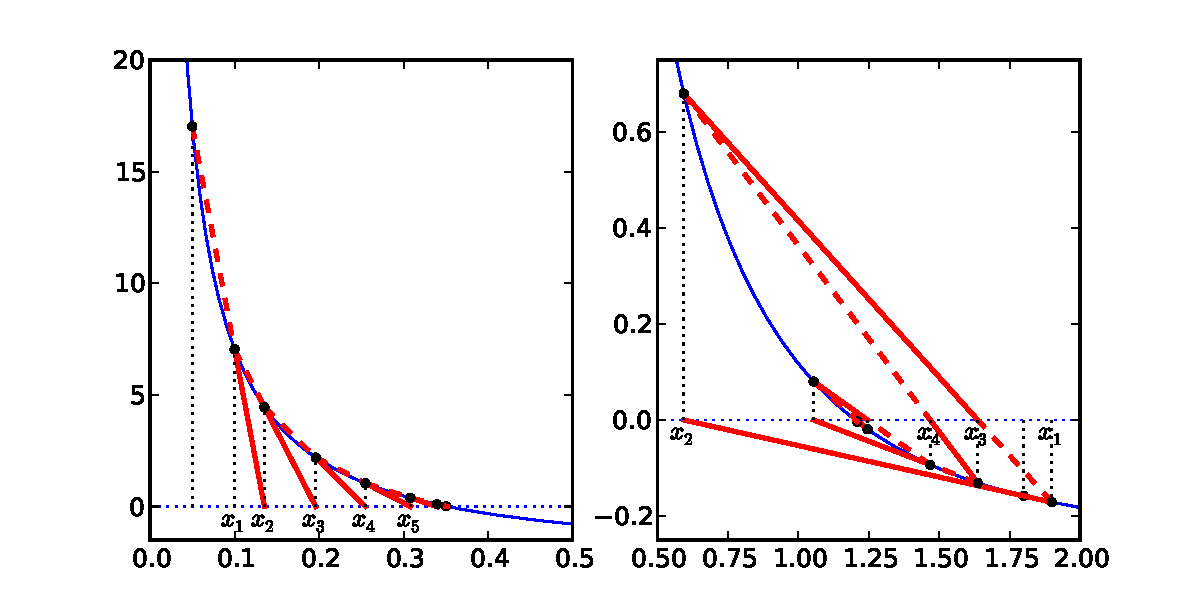
\includegraphics[width=\textwidth]{plots/sekanten}
  \caption{Sekantenmethode für die Funktion $f(r) = e^{-r}/r -
    \phi_0$. Wie zuvor ist links $\phi_0=2$, rechts $\phi_0=1/4$.
    Blau dargestellt ist wieder $f$, die roten, gestrichelten dicken
    Linien stellen die Sekanten dar, deren Nullstellen die neuen
    Näherungen für die gesuchte Nullstelle von $f$ sind. Durchgezogen
    ist der Abschnitt der Sekante durch $x_{n-1}$ und $x_n$, der von $x_n$
    zu $x_{n+1}$ führt.}
  \label{fig:sekanten}
\end{figure}

In vielen Fällen ist es nicht einfach oder unmöglich, die Ableitung
einer Funktion zu bestimmen. In diesem Fall kann man die Ableitung
durch die dividierte Differenz annähern, wobei nun zwei Startpunkte
$x_0$ und $x_1$ gebraucht werden. Dies führt dazu, dass die
Näherungsfunktion keine Tangente mehr ist, wie beim Newtonverfahren,
sondern im Allgemeinen eine Sekante. Daher rührt der Name der
\emph{Sekantenmethode}
\begin{equation}
  x_{n+1} = x_n - f(x_n)\frac{x_n - x_{n-1}}{f(x_n) - f(x_{n-1})},
\end{equation}
die nicht mehr quadratisch, aber wenigstens superlinear konvergiert.

Das Bestimmen der Ableitung von $f$ ist immer dann unmöglich, wenn $f$
sehr komplex ist. Ein Extremfall wäre eine
Molekulardynamik-Computersimulation, bei der zum Beispiel in
Abhängigkeit vom aktuellen Volumen $V$ der mittlere Druck $P(V)$ in
einem gegebenen System bestimmt wird. Den mittleren Druch nach $V$
abzuleiten, ist vollkommen aussichtslos, wenn die Wechselwirkungen
zwischen den Teilchen hinreichend komplex sind. Dabei ist es von
großem Interesse, dasjenige Volumen zu bestimmen, für das $P(V)$
gleich einem vorgegebenen Außendruck $P_0$ ist, denn dies ist die
natürliche Bedingung im isobarischen Ensemble. Dies führt aber zur
Nullstellengleichung $P(V)-P_0 = 0$.

Als Beispiel für die Sekantenmethode soll ein weiteres Mal die
Funktion $f(r) = e^{-r}/r - \phi_0$ dienen. Für diese zeigt
Abbildung~\ref{fig:sekanten} die erste paar Schritte der
Sekantenmethode. Unter geeigneten Umständen, nämlich, wenn die
angenäherte Tangente hinreichend gut mit der tatsächlichen über
einstimmt, konvergiert die Sekantenmethode praktisch genauso gut wie
das normale Newtonverfahren. Sind die Startpunkte allerdings ungünstig
gewählt, wie im rechten Beispiel, so kann es passieren, dass diese
abwechselnd um die Nullstelle liegen, und damit nicht mehr monoton
konvergieren.

In SciPy implementiert \scipy{scipy.optimize.newton(f, x0)} (also bei
Nichtangabe der Ableitung) die Sekantenmethode. \argd{f} ist wieder
die Funktion, deren Nullstelle gesucht wird, und \argd{x0} ein
Startwert. Der zweite wird hardcodiert in einer Umgebung von \argd{x0}
gewählt, kann also vom Benutzer nicht gesetzt werden.

\section{\keyword{Bisektion}}
\index{Bisektionsverfahren}

Wie wir gesehen haben, konvergiert das Newtonverfahren und seine
Varianten sehr schnell, allerdings oft nur unter der Voraussetzung,
dass der Startwert hinreichend nah an einer Nullstelle liegt. Wie aber
kann man einen solchen Startwert finden? Hierfür wird ein langsameres,
robusteres Verfahren gebraucht, zum Beispiel das
\emph{Bisektionsverfahren} in einer Dimension.

Sei also wieder $f\in C([a,b])$ eine stetige Funktion, und
$f(a)f(b)<0$. Dann hat $f$ gemäß Mittelwertsatz wenigstens eine
Nullstelle im Interval $[a,b]$, die wir suchen. Dazu setzen wir
zunächst $a_0=a$ und $b_0=b$. Dann betrachten wir den
Intervallmittelpunkt
\begin{equation}
  m_{n} = \frac{a_n + b_n}{2}.
\end{equation}
Ist $f(m_n)f(a_n) < 0$, hat die Funktion also bei $m_n$ und $a_n$ unterschiedliche Vorzeichen, so
muss eine Nullstelle im halb so großen Interval $a_1=a_0$, $b_1=m_0$
liegen, mit dem wir nun weiter verfahren. Anderfalls ist
notwendigerweise $f(m_n)f(b_n)\le 0$, und die Nullstelle ist im neuen
Interval $a_1=m_0$, $b_1 = b_0$. Ist $b_n - a_n$ kleiner als die
gewünschte Genauigkeit für die Nullstelle, bricht man einfach
ab. $m_n$ ist dann die endgültige Näherung für die Nullstelle.

Das Verfahren halbiert in jedem Schritt die Intervallgröße und damit
auch den maximalen Abstand der Näherung zur tatsächlichen
Nullstelle $\overline{x}$. Es gilt also
\begin{equation}
  \frac{\abs{m_{n+1} - \overline{x}}}{\abs{m_{n} - \overline{x}}}\le \frac{1}{2},
\end{equation}
das Verfahren konvergiert also nur linear, dafür aber global.

In der Praxis kombiniert man die Bisektion mit dem Newtonverfahren, indem
zunächst einige Schritte des Bisektionsverfahrens durchgeführt
werden, und dann vom Intervallmittelpunkt aus das
Newtonverfahren. Konvergiert dieses, so ist man fertig. Läuft das
Newtonverfahren aus dem Bisektionsinterval heraus,
verkleinert man dieses durch weitere Bisektionsschritte, und versucht dann
erneut, das Newtonverfahren anzuwenden.

In Abbildung~\ref{fig:bisektion} dient uns ein letztes Mal die
Funktion $f(x) = e^{-r}/r - 2$ als Beispiel für die Bisektion. Mit
sieben Schritten schließt diese bei Startinterval $[0,1,\,1]$ die
Nullstelle bis auf $[0,3391,\,0,3461]$, als etwa $10^{-2}$ genau
ein. Zum Vergleich: das Newtonverfahren mit Startwert $0,05$ erreicht
in sieben Schritten eine Genauigkeit von etwa $10^{-5}$, und selbst
die Sekantenmethode $10^{-3}$.
Der Vorteil der Bisektion ist aber, dass diese Methode im Allgemeinen
auch noch einigermaßen zufriedenstellend funktioniert, falls nicht nur
die Ableitungen unbekannt sind, sondern sogar die Funktionswerte gar
nicht genau bekannt sind. Dies wäre zum Beispiel bei der bereits
angesprochenen Messung des Drucks in einer Simulation der Fall, da
dieser starken Schwankungen unterliegt. Dadurch kann man meist den
Druck in akzeptabler Rechenzeit nicht so gut mitteln, dass dessen
Messfehler vernachlässigt werden kann. Die Bisektion muss in diesem
Fall schon abgebrochen werden, sobald der Funktionswert an einer der
Grenzen innerhalb des Fehlerbalkens Null ist.

In SciPy implementiert \scipy{scipy.optimize.bisect(f, a, b)} mit der
Funktion \argd{f} und Intervalgrenzen \argd{a} und \argd{b} die
Bisektion. \scipy{scipy.optimize.brentq(f, a, b)} implementiert die
Brentsche Methode, die unter den selben Bedingung wie die Bisektion
konvergiert, aber meist wesentlich schneller.

\begin{figure}
  \centering
  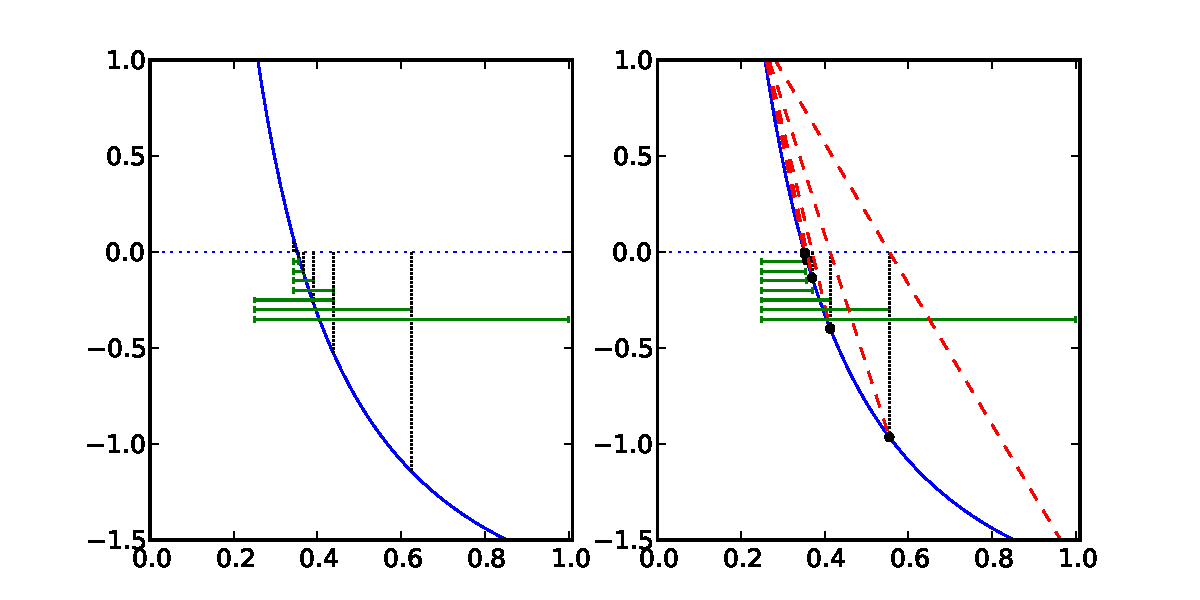
\includegraphics[width=\textwidth]{plots/bisektion}
  \caption{Links: Bisektion für die Funktion $f(r) = e^{-r}/r -
    \phi_0$, hier nur mit $\phi_0=2$, da die genaue Form der Funktion
    für diese Methode unerheblich ist. Blau dargestellt ist wieder
    $f$, die grünen Balken markieren die nacheinander generierten,
    kleiner werdenden Intervalle $[a_n, b_n]$. Die gestrichelten,
    schwarzen Linien markieren die Intervalmitten $m_n$, die im
    nächsten Schritt eine der beiden Intervalgrenzen werden. Rechts:
    Regula falsi für dieselbe Funktion. Die Funktion ist streng
    konvex, daher reagiert die Regula falsi lethargisch und ist der
    Bisektion unterlegen; die Intervalle verkürzen sich praktisch
    nicht mehr, da die untere Anfangsgrenze $1/4$ nie versetzt wird,
    nur die obere Grenze.}
  \label{fig:bisektion}
\end{figure}

\section{\keyword{Regula falsi}}

Sowohl die Bisektion wie auch die Sekantenmethode benötigen zwei
Startwerte. Daher liegt es nahe, die Verfahren zu kombinieren.
Bei der \emph{Regula falsi} wird wie bei der Bisektion ein Interval
$[a,b]$ schrittweise verkleinert so dass dieses stets wenigstens eine
Nullstelle enthält. Anders als bei der Bisektion wird der neue
Randpunkt $m$ allerdings nicht einfach als Intervalmitte bestimmt,
sondern mit Hilfe der Sekantenmethode, mit den beiden
Intervalrandpunkten $a$ und $b$ als Stützstellen:
\begin{equation}
  m = b - f(b)\frac{b - a}{f(b) - f(a)} =
  \frac{f(b)a - f(a)b}{f(b) - f(a)}.
\end{equation}
Da $f(a)f(b)<0$, schneidet die Sekante die Nulllinie immer im
Interval.  Dadurch verkleinert sich das Interval schneller als beim
Bisektionsverfahren, sofern die Nullstelle der Sekante dicht an der
echten Nullstelle liegt. Hat die Funktion im Intervall allerdings
einen Wendepunkt, ist also nicht streng konkav oder konvex, dann wird
die Regula falsi sehr langsam, was auch als Lethargie bezeichnet
wird. Der Grund ist, dass eine der beiden Intervallgrenzen sehr dicht
an die Nullstelle rückt, und im folgenden nur noch diese Grenze
minimal verbessert wird, während die zweite Grenze unverändert
bleibt. Dies ist zum Beispiel in Abbildung~\ref{fig:bisektion} rechts
gezeigt. Leider sind nicht streng konkave oder konvexe Funktionen eher
die Regel als die Ausnahme, daher ist die einfache Bisektion oft
schneller als die Regula falsi.  Die Regula falsi ist nur dann die
schnellste und stabilste Nullstellensuche, falls die Ableitung der
Funktion nicht bekannt ist, man aber weiß, dass die Funktion streng
konvex oder konkav ist.

\section{Newtonverfahren in mehreren Dimensionen}
\index{Newtonverfahren>in mehreren Dimensionen}
\index{Gleichungssysteme>nichtlineare}

Bis jetzt haben wir das Newtonverfahren nur für eindimensionale
Funktionen betrachtet. Im mehrdimensionalen funktioniert das Verfahren
aber sehr ähnlich, wobei die Ableitung zur Jacobimatrix wird.

Sei also $f\in C^1(M, \RR^n)$ eine stetig differenzierbare Abbildung
von $M\in\RR^n$ in den $\RR^n$. Wir suchen nun eine Nullstelle
$\overline{x}\in D$, \dh eine Lösung des nichtlinearen
Gleichungssystems $f(x) = 0$.

Wie schon im Eindimensionalen starten wir mit einer Näherung
$x^{(0)}\in M$, und berechnen die nächste Näherung $x^{(1)}$ durch
Linearisieren von $f$ in $x^{(0)}$. Die Linearisierung ergibt sich aus
der Taylorentwicklung:
\begin{equation}
  \label{eq:linnewton}
  F(x^{(1)}) \,\dot{=}\, F(x^{(0)}) +
  F'(x^{(0)})\left(x^{(1)}-x^{(0)}\right),
\end{equation}
wobei
\begin{equation}
  F'(x) = \left(\frac{d}{dx_j}F_k(x)\right)_{k,j} = 
  \begin{pmatrix}
    \frac{d}{dx_1}F_1(x) & \ldots & \frac{d}{dx_n}F_1(x)\\
    \vdots               &        & \vdots \\
    \frac{d}{dx_1}F_n(x) & \ldots & \frac{d}{dx_n}F_n(x)
  \end{pmatrix}
\end{equation}
die \emph{\keyword{Jacobimatrix}} von $f$ an der Stelle $x$ bezeichnet.
Die neue Näherung $x^{(1)}$ suchen wir als Nullstelle der
Linearisierung \eqref{eq:linnewton}, also aus der Bedingung
$F(x^{(1)})\stackrel{!}{=} 0$. Da wir ja damit nur die
linearisierte Gleichung gelöst haben, linearisieren wir erneut im
neuen Punkt $x^{(1)}$, und so weiter. Ein Schritt des Newtonverfahrens
ist dann also
\begin{equation}
  x^{(m+1)} = x^{(m)} + d^{(m)}\quad\text{mit}\;
  F'(x^{(m)})\,d^{(m)} = -F(x^{(m)}).
\end{equation}
Die \emph{Newtonkorrektur} $d^{(m)}$ wird als aus der Lösung eines
linearen Gleichungssystems gewonnen, zum Beispiel mit Hilfe der
Gaußelimination. Allerdings ist $f'$ im Allgemeinen vollbesetzt, daher
verwendetet man normalerweise schnellere, approximative Verfahren, die
wir später kennenlernen werden. Ist $F'(x^{(m)})$ in einem Schritt
singulär, so bricht das Verfahren ab. Ansonsten wird weiter iteriert,
bis $\norm{d^{(m)}}$ hinreichend klein ist.

Auch im mehrdimensionalen konvergiert dieses Verfahren lokal
mindestens quadratisch, sofern in einer abgeschlossenen Umgebung der
Nullstelle $\norm{F'(x)^{-1}}$ beschränkt ist und $f$ zweifach stetig
differenzierbar. Allerdings gibt es kein langsames Verfahren ähnlich
der Bisektion, dass man dem Vefahren vorausschicken könnte, um die
Nullstelle einzugrenzen. Die globale Suche nach Nullstellen in
mehreren Dimensionen ist also eine schwierige Aufgabe. Eine
Möglichkeit ist, zunächst mit Hilfe von Optimierungsverfahren ein
$x_0$ zu finden mit möglichst kleiner Norm $\norm{f(x_0)}$, und von
dort das (gedämpfte) Newtonverfahren zu starten. Die globale
Optimierung in vielen Dimensionen ist selber eine sehr schwierige
Aufgabe, allerdings existieren hierfür Ansätze wie genetische
Algorithmen oder Simulated Annealing, die wir später kennenlernen
werden.

\subsection{Gedämpftes Newtonverfahren}
\index{Newtonverfahren>gedämpftes}

Leider ist im Mehrdimensionalen die Umgebung um die Nullstelle, in der
das Verfahren konvergiert, oftmals deutlich kleiner. Das Verfahren
springt dann leicht über die Nullstelle hinweg, wie es im
eindimensionalen nur am Anfang des Verfahrens vorkommt
(\zb Abbildung~\ref{fig:newton} rechts, im ersten Schritt). Um dies
zu verhindern, kann man die Schrittweite reduzieren, als den Schritt
$d^{(m)}$ verkürzen. Die Iteration lautet dann
\begin{equation}
  x^{(m+1)} = x^{(m)} + \lambda d^{(m)}\quad\text{mit}\;
  F'(x^{(m)})\,d^{(m)} = -F(x^{(m)}),
\end{equation}
wobei die Dämpfung $\lambda\in (0,1]$ so gewählt wird, dass
$\norm{F(x^{m+1})}\le\norm{F(x^{m})}$. Dazu wird zum Bespiel mit
$\lambda=1$ begonnen, und $\lambda$ solange verringert, bis die
Bedingung erreicht ist.

\begin{lstlisting}[style=floating,deletekeywords={lambda},
caption={Gedämpftes Newtonverfahren in mehreren
Dimensionen. \lstinline!f(x)! muß
eine vektorwertige Funktion sein, \lstinline!fprime(x)! ihre
Ableitung, d.h. eine matrixwertige Funktion.}]
# Gedaempftes Newtonverfahren
#############################

def gedaempfter_newton(f, fprime, x0, epsilon):
   xn = x0
   konvergiert = False
   while not konvergiert:
      # Newton-Korrektur
      dn = solve(fprime(xn), f(xn))
      if norm(dn) < epsilon:
         konvergiert = True
      else:
         # Schrittweitendaempfung
         lambda = 1.0
         abstieg = False
         while not abstieg:
            # neue Naeherung
            xneu = xn + lambda*dn
            if norm(f(xneu)) < norm(f(xn)):
               abstieg = True
            else:
               lambda = lambda / 2.0
         xn = xneu
   return xn
\end{lstlisting}

%%% Local Variables: 
%%% mode: latex
%%% TeX-master: "padc"
%%% TeX-PDF-mode: t
%%% End: 

% Dies ist Teil der Vorlesung Physik auf dem Computer, SS 2012,
% Axel Arnold, Universitaet Stuttgart.
% 
% Dieses Werk ist unter einer Creative Commons-Lizenz vom Typ
% Namensnennung-Weitergabe unter gleichen Bedingungen 3.0 Deutschland
% zugänglich. Um eine Kopie dieser Lizenz einzusehen, konsultieren Sie
% http://creativecommons.org/licenses/by-sa/3.0/de/ oder wenden Sie sich
% schriftlich an Creative Commons, 444 Castro Street, Suite 900, Mountain
% View, California, 94041, USA.

\chapter{Numerisches Differenzieren und Integrieren}

In diesem Kapitel geht es darum, wie eine Funktion, die an diskreten
Stützstellen gegeben ist, numerisch differenziert und integriert
werden kann. Die Grundlagen dazu wurden bereits mit dem Kapitel
``Darstellung von Funktionen'' gelegt: für die numerische Ableitung
liegt es nahe, aus der Taylorentwicklung geeignete Ausdrücke für die
Ableitungen zu gewinnen, und für die Integration bieten sich das
interpolierende Polynom oder auch ein Spline and, die sich mit dem
Computer leicht analytisch integrieren lassen.

Numerisches Integrieren und Differenzieren kann dabei nicht nur dazu
dienen, Integrale oder Ableitungen abzuschätzen, sondern erlaubt auch,
einfache Differential- oder Integralgleichungen numerisch zu
lösen. Dazu muss die Gleichung mit Hilfe der hier vorgestellten
Verfahren diskretisiert und das resultierende lineare Gleichungssystem
gelöst werden.

\section{Numerisches Differenzieren}
\index{Differenzieren}

Die erste Ableitung einer Funktion $f\in C^1([a,b])$ ist definiert als
\begin{equation}
  \lim_{h\to 0} \frac{f(x+h) - f(x)}{h}.
\end{equation}
Um den Grenzwert abzuschätzten, liegt es nahe, die Ableitung durch die
dividierte Differenz
\begin{equation}
  f'(\xi) \approx f[x,y] := \frac{f(x) - f(y)}{x - y}
\end{equation}
anzunähern, wobei $x$ und $y$ beide nahe bei $\xi$ liegen sollten.

Doch an welchem Punkt $\xi$ ist diese Näherung optimal? Gemäß
Mittelwertsatz gilt auf jeden Fall $f[x,y]=f'(\xi)$ für ein $\xi\in
[x,y]$. Man erwartet daher, dass $f[x,y]$ am besten in der
Intervallmitte $m=\frac{x+y}{2}$ approximiert. Das ist tatsächlich so,
wie wir nun per Taylorentwicklung sehen werden. Mit Entwicklung um $m$
und $h=x-y$ gilt
\begin{align}
  \frac{f(x) - f(y)}{x-y} &= \frac{1}{h}
  \biggl(+f(m) + \frac{h}{2}f'(m) + \frac{h^2}{8}f''(m) + \O(h^3)\nonumber\\
  &\phantom{= \frac{1}{h}\biggl(}-f(m) + \frac{h}{2}f'(m) - \frac{h^2}{8}f''(m) + \O(h^3)
  \biggr)\nonumber\\
  &=  f'(m) + \O(h^2).
\end{align}
Bei Ansatzpunkt $x$ gilt hingegen nur
\begin{align}
  \frac{f(x) - f(y)}{x-y} = \frac{1}{h}
  \biggl(f(x) + h f'(x) + \frac{h^2}{8}f''(x) + \O(h^3) - f(x) \biggr)
  =  f'(x) + \O(h).
\end{align}

In der Praxis ist die Funktion meist an an äquidistanten Stützstellen
$x_i$ mit $x_{i+1}-x_i=h$ gegeben. Dann ist, wie oben gezeigt, die
beste Zweipunkt-Näherung für die Ableitung die zentrale Differenz
\begin{equation}
  \label{eq:2orderdiff}
  \frac{f(x_{i+1}) - f(x_{i-1})}{2h} = f[x_{i-1},x_{i+1}] = f'(x_i) + \O(h^2),
\end{equation}
während für die linken und rechten dividierten Differenzen gilt:
\begin{equation}
  \frac{f(x_{i+1}) - f(x_{i})}{h} = f[x_{i},x_{i+1}] = f'(x_i) + \O(h)
\end{equation}
bzw.
\begin{equation}
  \frac{f(x_{i}) - f(x_{i-1})}{h} = f[x_{i},x_{i-1}] = f'(x_i) + \O(h).
\end{equation}

\subsection{Näherungen höhererer Ordnung und höhere Ableitungen}

Mit Hilfe von Taylorentwicklungen lassen sich auch Näherungen mit mehr
Stützpunkten und für höhere Ableitungen entwickeln.  Wir betrachten
zum Beispiel die Punkte für $k=-2(1)2$, d.h.\ die 5 benachbarten
Punkte, und suchen Koeffizienten $c_k$ derart, dass
\begin{equation}
  c_2 f(x_{i+2}) + c_1 f(x_{i+1})  + c_0 f(x_i) + c_{-1}f(x_{i-1}) +
  c_{-2}f(x_{i-2}) = f'(x_i) + \O(h^5),
\end{equation}
unabhänging von der Form von $f$ und seiner Ableitungen. Durch
Einsetzen der Taylorentwicklung
\begin{equation}
  f(x + k h) = f(x) + k\, hf'(x) + k^2\,\frac{h^2}{2} f''(x_i) +
  k^3\,\frac{h^3}{6}f^{(3)}(x) + k^4\,\frac{h^4}{24}f^{(4)}(x) + \O(h^5)
\end{equation}
können wir nun die obige Gleichung auf beiden Seiten als Vielfache von
$f(x)$, $f'(x)$, $f''(x)$ usw.\ schreiben. Da unsere Koeffizienten
unabhängig von diesen sein sollen, müssen die Vorfaktoren vor diesen
auf beiden Seiten übereinstimmen. Diese sind, beginnend bei $f(x)$:
\begin{align}
  \label{eq:derivatives}
  c_{2} + c_{-2} + c_{-1} + c_1 + c_0 &= 0\nonumber\\
  h\left[2 (c_{2} - c_{-2})  + c_{1} - c_{-1}\right] &= 1\nonumber\\
  \frac{h^2}{2}\left[4(c_{2} + c_{-2})  + c_{1} + c_{-1}\right] &= 0\nonumber\\
  \frac{h^3}{6}\left[8 (c_{2} - c_{-2})  + c_{1} - c_{-1}\right] &= 0\nonumber\\
  \frac{h^4}{24}\left[16 (c_{2} + c_{-2}) + c_{1} + c_{-1}\right] &= 0.
\end{align}
Durch Lösen des Gleichungssystems folgt
\begin{equation}
  \label{eq:4orderdiff}
  -\frac{1}{12h} f(x_{i+2}) + \frac{2}{3h} f(x_{i+1})  - \frac{2}{3h} f(x_{i-1}) +
  \frac{1}{12h}f(x_{i-2}) = f'(x_i) + \O(h^4).
\end{equation}
Auf diese Weise lässt sich auch die höhere Güte der zentralen
Differenz verstehen: tatsächlich entspricht diese der optimalen
Näherung durch $x_{i-1}$, $x_i$  und $x_{i+1}$, nur dass aus
Symmetriegründen der Koeffizient zu $x_i$ verschwindet.

Um nun zum Beispiel die zweite Ableitung zu berechnen, lösen wir
\eqref{eq:derivatives}, allerdings mit einer 1 nicht in der zweiten,
sondern dritten Zeile. Das ergibt
\begin{equation}
  \label{eq:3order2diff}
  \frac{1}{h^2}\left(-\frac{1}{12} f(x_{i+2}) + \frac{4}{3} f(x_{i+1}) +
  \frac{5}{2} f(x_i)  + \frac{4}{3} f(x_{i-1}) -
  \frac{1}{12}f(x_{i-2})\right) = f''(x_i) + \O(h^4).
\end{equation}
Die Fehlerordnung ist hier um eins höher als man erwarten würde, da für den
Term dritter Ordnung der Vorfaktor ebenfalls verschwindet:
\begin{equation}
  \frac{1}{12} \cdot 8 - \frac{4}{3} +
  \frac{4}{3} - \frac{1}{12}\cdot 8 = 0.
\end{equation}

Mit drei Stützpunkten ergibt sich die Näherung für die zweite
Ableitung analog als
\begin{multline}
  \label{eq:1order2diff}
  \frac{1}{h^2}\bigl(f(x_{i+1}) -
  2f(x_i)  + f(x_{i-1})\bigr) =
  \frac{\frac{f(x_{i+1}) - f(x_i)}{h}  -
    \frac{f(x_i) - f(x_{i-1})}{h}}{h}
  = f''(x_i) + \O(h^2).
\end{multline}
Die mittlere Form zeigt, dass sich diese einfachste Form der zweiten
Ableitung auch als dividierte Differenz der dividierten Differenzen
verstehen lässt. Technisch wird also die zweite Ableitung also einfach
in erster Ordnung aus der ersten Ableitung in erster Ordnung
bestimmt. Analog lässt sich jede $n$-te Ableitung aus $n+1$
benachbarten Stützstellen in erster Ordnung durch dividierte
Differenzen approximieren.

\subsection{Genauigkeit}

\begin{figure}
  \centering
  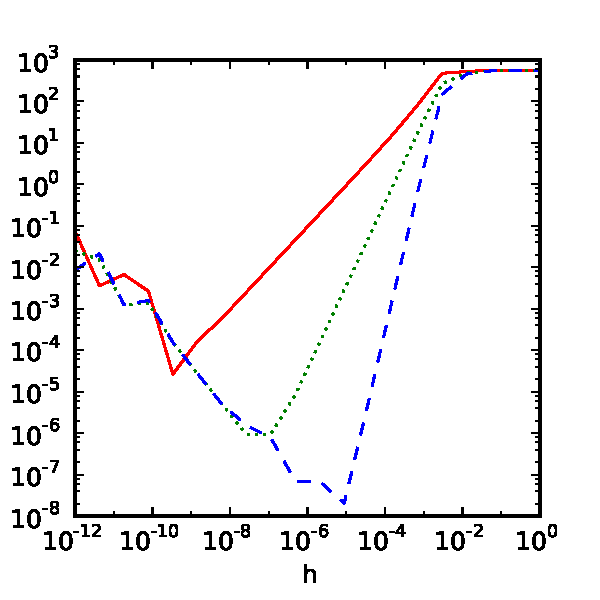
\includegraphics[width=0.5\textwidth]{plots/num_diff}
  \caption{Maximale Abweichung $\max_{x\in[-\pi,pi]} \abs{f'(x) - a(h;
      x)}$ für verschiedene Näherungen $a(h; x)$, als Funktion der
    Schrittweite $h$. Die Funktion ist $f(x)=sin(100x^2)$. Rot
    durchgezogen ist die linksseitige Differenz $a(h; x) = (f(x) -
    f(x-h))/h$, die zentrale Differenz $a(h; x) = (f(x+h) -
    f(x-h))/2h$ ist grün gepunktet und die Näherung 4. Ordnung
    \eqref{eq:4orderdiff} blau gestrichelt. Der rechtsseitige Abfall
    der Kurven entspricht den Ordnungen $\O(h)$ für die linksseitige
    Differenz, $\O(h^2)$ für die rechtsseitige und $\O(h^4)$ für die
    Gleichung 4. Ordnung. Das linksseitige Verhalten ist
    methodenunabhängig und durch die endliche Rechenauflösung bestimmt.}
  \label{fig:num_diff}
\end{figure}

Generell sind alle diese Näherungen numerisch instabil, da bei kleinen
Abständen $h$ auch $f(x)$ und $f(x+h)$ sehr ähnlich sind. Sind diese
betragsmäßig groß, kommt es zu Auslöschung, d.h., $f(x+h) - f(x)$ hat
deutlich weniger signifikante Stellen als Maschinengenauigkeit. Daher
gibt es stets ein optimales $h$, das allerdings von der unbekannten
zweiten Ableitung der betrachteten Funktion abhängt.

Auch Verfahren höherer Ordnung sind nicht notwendigerweise genauer, da
bei manchen Funktionen die Ableitungen sehr rasch wachsen. Dann ist
zwar $h^4$ sehr viel kleiner als $h^2$, aber der Vorfaktor
kompensiert das zunächst. Abbildung~\ref{fig:num_diff} illustriert
dieses Verhalten am Beispiel der Funktion $\sin(100x^2)$. Erst, wenn
die Schrittweite $h$ unter die charakteristische Breite von etwa 600
sinkt, spielt die Ordnung des Verfahrens eine Rolle. Wird allerdings
$h$ zu klein, zeigt sich die endliche Auflösung, mit der der Rechner
arbeitet, und der Fehler steigt wieder an.

\subsection{Beispiel: Besselsche Differentialgleichung}

\begin{figure}
  \centering
  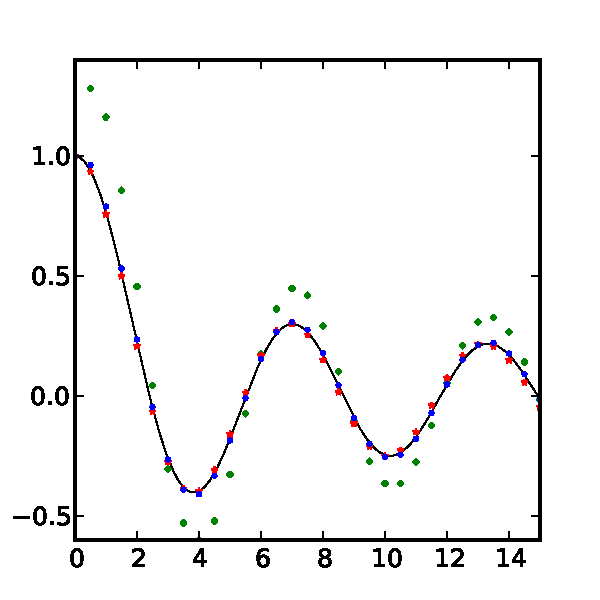
\includegraphics[width=0.5\textwidth]{plots/bessel_diff}
  \caption{Numerische Lösungen der Besselschen Differentialgleichung
    auf $[0,15]$ mit Schrittweite $h=0,5$ und $N=31$ Stützpunkten. Die
    durchgezogene schwarze Linie markiert die analytische Lösung. Mit
    grünen Diamanten ist die Lösung mit Hilfe von
    \eqref{eq:besseldiscrete} und Dirichletrandbedingungen
    dargestellt, für die roten Sterne wurden Funktionswert und
    Ableitung bei $0$ festgelegt. Blaue Punkte schließlich markieren
    den Löser dritter Ordnung mit Dirichletrandbedingungen, der von
    der analytischen Lösung praktisch nicht zu unterscheiden ist.}
  \label{fig:bessel_diff}
\end{figure}

Wir betrachten die Besselsche Differentialgleichung, eine gewöhnliche
lineare Differentialgleichung zweiter Ordnung:
\begin{equation}
  \label{eq:besselode}
  x^2\frac{d^2f}{dx^2} + x\frac{df}{dx} + (x^2-\nu)f = 0
\end{equation}
für $f\in C^{\infty}([0,\infty))$. Die Besselsche
Differentialgleichung spielt eine wichtige Rolle in der Physik, weil
sie den radialen Anteil der Laplacegleichung in Zylinderkoordinaten
beschreibt.  Für die Lösungen dieser Gleichung lassen sich schnell
konvergierende Reihen oder Integraldarstellungen
angeben~\cite{abramowitz70a,jackson99}, wir wollen aber zu
Demonstrationszwecken diese Differentialgleichung für $\nu=0$
numerisch lösen. Hierzu definieren wir $f_k := f(kh)$, $k\ge 0$, und
diskretisieren \eqref{eq:besselode} mit Hilfe der finiten Differenzen
\eqref{eq:2orderdiff} und \eqref{eq:1order2diff} in linearer Ordnung:
\begin{align}
  \label{eq:besseldiscrete}
  0 &= k^2\left(f_{k-1} - 2f_k + f_{k+1} \right)
  + k\left(\frac{1}{2} f_{k+1} - \frac{1}{2} f_{k-1}\right)
  + k^2h^2f_k\nonumber\\
  &= \left(k^2 - \frac{1}{2}k\right)f_{k-1}
  + k^2(h^2 - 2)f_k
  + \left(k^2 + \frac{1}{2}k\right)f_{k+1}.
\end{align}
Für die Lösung $f$ auf dem endlichen Intervall $[0, (N-1)h]$ sind das
$N-2$ Gleichungen, da zumindest für die Randpunkte die zweite
Ableitung so nicht abgeschätzt werden kann. Dies ist aber auch nicht
weiter verwunderlich, da wir ja die Randbedingungen noch nicht
festgelegt haben. Die natürlichen Randbedingungen der Diskretisierung
sind also Dirichlet-Randbedingungen, bei denen die fehlenden Randwerte
vorgegeben werden: $f_0 = f(0)=F_0$ und $f_{N-1} = f((N-1)h) = F_{N-1}$.

Wir erhalten das folgende lineare Gleichungssystem:
\begin{equation}
  \begin{pmatrix}
    1 & 0         & 0         &\ldots & \ldots & 0\\
    \nicefrac{1}{2} & -\lambda & \nicefrac{3}{2} & 0 & \ldots & 0\\
    0 & 3         & -4\lambda & 5 & 0\quad \ldots & 0\\
    & & \ddots & \ddots & \ddots\qquad\qquad \\
    0 & \ldots & 0 & \mu_n - \nu_n & -\mu_n\lambda & \mu_n + \nu_n\\
    0 &          &  \ldots  &   & 0      & 1
  \end{pmatrix}
  \begin{pmatrix}
    f_0\\
    \vdots\\
    f_{N-1}
  \end{pmatrix}=
  \begin{pmatrix}
    F_0\\
    0\\
    0\\
    \vdots\\
    0 \\
    F_{N-1}
  \end{pmatrix},
\end{equation}
wobei $\lambda=(2-h^2)$, $\mu_n=(N-2)^2$ und $\nu_n=
\frac{1}{2}(N-2)$. Die beiden äußeren Zeilen implementieren die
Dirichletbedingungen, die restlichen Zeilen Gleichung
\eqref{eq:besseldiscrete} für $k=1(1)N-1$.  Da die Matrix Bandstruktur
hat, können wir dieses lineare Gleichungssystem effizient mit dem
Gaußverfahren lösen.

Beispielcode~\ref{lst:bessel} zeigt ein Pythonskript zur Lösung dieses
Gleichungsssystems. Dessen Lösung für $h=0,5$ ist in
Abbildung~\ref{fig:bessel_diff} mit grünen Diamanten gezeigt und
weicht noch signifikant ab, was allerdings durch die hohe Schrittweite
bedingt ist. Mit einer Schrittweite $h < 0,1$ gäbe es keine sichtbaren
Abweichungen mehr.

Alternativ können wir statt der Dirichlet-Randbedingungen auch
Funktion $f(0) = F_0$ und Ableitung $f'(0)=F'_0$ am linken Rand
festlegen. Das ergibt:
\begin{equation}
  \begin{pmatrix}
    1 & 0         & 0         &\ldots & \ldots & 0\\
    -\nicefrac{1}{2h} & 0         & \nicefrac{1}{2h} &\ldots & \ldots & 0\\
    \nicefrac{1}{2} & -\lambda & \nicefrac{3}{2} & 0 & \ldots & 0\\
    0 & 3         & -4\lambda & 5 & 0\quad \ldots & 0\\
    & & \ddots & \ddots & \ddots\qquad\qquad \\
    0 & \ldots & 0 & \mu_n - \nu_n & -\mu_n\lambda & \mu_n + \nu_n\\
  \end{pmatrix}
  \begin{pmatrix}
    f_0\\
    \vdots\\
    f_{N-1}
  \end{pmatrix}=
  \begin{pmatrix}
    F_0\\
    F'_0\\
    0\\
    \vdots\\
    0 \\
  \end{pmatrix}.
\end{equation}
Abbildung~\ref{fig:bessel_diff} zeigt, dass die Lösung in diesem Fall
am linken Rand genauer ist, während sie zum rechten Rand hin
abweicht. Das ist ist zu erwarten, da unsere Bedingung die Lösung ja
nur am linken Rand zwingen, mit der analytischen Lösung
übereinzustimmen.

Generell zeigen allerdings sowohl Dirichlet- wie auch gemischte
Randbedingungen noch leichte Artefakte. Diese lassen sich durch
natürlich durch kleinere Schrittweite verringern, da die Lösung aber
$C^\infty$ ist, kann man aber stattdessen auch auf
Ableitungsnäherungen höherer Ordnung zurückzugreifen, etwa
\eqref{eq:3order2diff} und \eqref{eq:4orderdiff}. Dann ist die
Hauptgleichung
\begin{align}
  0 = &\frac{1}{12}(-k^2 + k)f_{k-2}
  + \frac{2}{3}(2k^2 - k)f_{k-1}
  + k^2\left(h^2 - \frac{5}{2}\right)f_k\nonumber\\
  &+ \frac{2}{3}(2k^2 - k)f_{k+1}
  + \frac{1}{12}(-k^2 + k)f_{k+2}.
\end{align}
Bei $N$ Punkten lassen sich hierdurch nur $N-4$ Gleichungen
formulieren, weil ja am linken und rechten Rand jeweils noch zwei
Nachbarpunkte benötigt werden. Von diesen benutzen wir zwei zum
Beispiel als Dirichletbedingungen $f_0 = F_0$ und $f_{N-1} = F_{N-1}$,
und generieren daraus über Gleichung \eqref{eq:besseldiscrete}
Näherungen für $f_1$ und $f_{N-2}$. Die Lösung dieses Gleichungssystem
ist in Abbildung~\ref{fig:bessel_diff} blau gepunktet eingezeichnet
und fast nicht mehr von der analytischen Lösung zu unterscheiden. Dies
zeigt den Nutzen von Ableitungsnäherungen höherer Ordnung.

\afterpage{\raggedbottom
  \lstinputlisting[style=multipage,firstline=10,
  caption={Numerische Lösung der Besselschen Differentialgleichung mit
    Hilfe von finiten Differenzen linearer und kubischer Ordnung. Dieser
    Code erzeugt Abbildung~\ref{fig:bessel_diff}},
  label=lst:bessel]{bessel.py}
  \clearpage
}

\section{\keyword{Quadratur}: \keyword{numerische Integration}}
\index{Integration>numerische}

Bei der numerischen Integration geht es genau wie beim Differenzieren
darum, aus endlich vielen Stützwerten das Integral einer Funktion in
einem endlichen Intervall abzuschätzen. Wir suchen also Gewichte
$\alpha_{i}\in\RR$, so dass möglichst genau
\begin{equation}
  \int_a^b f(x)\, dx \approx \sum_{i=0}^{n-1} \alpha_if(x_i),
\end{equation}
wobei die $\alpha_i$ von der Lage der Stützpunkte ("`Knoten"') $x_i$
abhängen, aber nicht von $f$. Dadurch, dass die Funktion über dem
ganzen Intervall $[a,b]$ in das Integral eingeht, wird man für die
numerische Integration natürlich mehr Punkte als beim Differenzieren
einbeziehen wollen, und hat dementsprechend auch mehr Möglichkeiten,
die Gewichte zu wählen. Im folgenden werden wir einige der
gebräuchlichsten Verfahren kennenlernen.

\subsection{\keyword{Newton-Cotes-Formeln}}
\index{Integration>Newton-Cotes-Formeln}

Um eine an diskreten Stützstellen $x_i$, $i=0(1)n-1$ gegebene Funktion
$f$ zu integrieren, liegt es nahe, die Funktion mit Hilfe eines
Polynoms zu interpolieren und dieses dann analytisch zu integrieren:
\begin{equation}
  \int_a^b f(x)\, dx \approx
  \int_a^b \sum_{i=0}^{n-1} f(x_i) L_i(x) \, dx = \sum_{i=0}^{n-1}
  \underbrace{\int_a^b
  L_i(x) dx}_{\alpha_i}\, f(x_i).
\end{equation}
Diese \emph{Newton-Cotes-Formeln} integrieren offenbar alle Polynome
bis Ordnung $n$ exakt. Allerdings verstärkt sich bei allgemeinen
Funktion das Rungephänomen bei der Integration, und ab Ordnung $n=9$
treten negative Koeffizienten $\alpha_i$ auf, was die Näherung
verschlechtert. Daher sind nur kleine $n$ sinnvoll, und in der Praxis
werden nur Formeln bis Ordnung $n=8$ benutzt. Die
gebräuchlichsten werden im folgenden kurz diskutiert.

\newcommand{\topillu}[1]{%
  \begin{tikzpicture}[overlay,x=\textwidth,y=\baselineskip]
    \draw (1,3) node[anchor=north east] {\includegraphics[width=0.25\textwidth]{#1}};
  \end{tikzpicture}\\}

\subsubsection{\keyword{Trapezregel}}
\index{Integration>Trapezregel}
\topillu{plots/trapezregel}
\begin{minipage}{0.74\linewidth}
  Die Trapezregel benutzt als Stützstellen $x_0=a$ und $x_1=b$, die
  dementsprechend durch eine Gerade verbunden werden:
  \begin{align}
    \int_a^b f(x)\, dx &\approx \int_a^b f(a)\frac{x-b}{a-b} \,+\,
    f(b)\frac{x-a}{b-a}\,dx\nonumber\\
    &= f(a)\int_a^b \frac{x-b}{a-b}\,dx \,+\,
    f(b)\int_a^b \frac{x-a}{b-a}\,dx\nonumber\\
    &= \frac{b-a}{2} \Bigl(f(a) + f(b)\Bigr).
  \end{align}
\end{minipage}

\noindent Weiter gilt für den Fehler der Trapezregel
\begin{multline}
  \int_a^b f(x)\, dx - \frac{b-a}{2} \Bigl(f(a) + f(b)\Bigr)
  =  \int_a^b f(x) - f(a)\frac{x-b}{a-b}
  + f(b)\frac{x-a}{a-b}\, dx\\
  =  \int_a^b
  {}\bigl(f(x) - f(a)\bigr)\frac{x-b}{a-b}
  + \bigl(f(b) - f(x)\bigr)\frac{x-a}{a-b}\, dx\\
  =  \int_a^b
  \frac{1}{a-b}\left(\frac{f(x) - f(a)}{x-a} + \frac{f(b) - f(x)}{x-b}\right)
  \underbrace{(x-b)(x-a)}_{<0\;\text{in}\;[a,b]}\, dx\\
  =
  \frac{f''(\xi)}{2}\int_a^b (x-b)(x-a)\, dx = -\frac{(b-a)^3}{12} f''(\xi)
\end{multline}
für ein $\xi\in[a,b]$. Gibt es also eine Abschätzung für die zweite
Ableitung von $f$, so lässt sich auch der Fehler der Trapezregel
abschätzen. Ist $f$ konvex auf $[a,b]$, also $f''(\xi)>0$, so
unterschätzt also die Trapezregel das Integral, ist $f$ konkav,
überschätzt sie es.

\subsubsection{\keyword{Simpsonregel}}
\index{Integration>Simpsonregel}
\topillu{plots/simpsonregel}
\begin{minipage}{0.74\linewidth}
  Analog wird die Simpsonregel für die drei Stützpunkte $x_0=a$,
  $x_1=m=\frac{a+b}{2}$ und $x_2=b$ definiert, die durch eine Parabel
  verbunden werden:
  \begin{align}
    \int_a^b f(x)\, dx &= \frac{b-a}{6} \left(f(a) +
      4 f\left(m\right) + f(b)\right)\nonumber\\
    &-\frac{(b-a)^5}{2880} f^{(4)}(\xi)
  \end{align}
  für ein $\xi\in[a,b]$, wobei der letzte Term wieder der Fehlerterm ist.
\end{minipage}

\index{Newton-Cotes-Formeln>offene}
\index{Newton-Cotes-Formeln>geschlossene}
Die Simpsonregel und die Trapezregel sind die meistgenutzten
\emph{geschlossenen} Newton-Cotes-Formeln. Geschlossen heißen solche
Formeln, die $a$ und $b$ als Stützpunkte beinhalten. \emph{Offene}
Formeln dagegen enthalten wenigstens einen der Punkte
nicht. Naturgemäß sind die beiden folgenden Einpunktformeln offen.

\subsubsection{\keyword{Rechteckregel}}
\index{Integration>Rechteckregel}
\topillu{plots/rechteckregel}
\begin{minipage}[t]{0.74\linewidth}
  Wir benutzen $x_0=a$ als Stützpunkt, und erhalten:
  \begin{equation}
    \int_a^b f(x)\, dx = (b-a) f(a) +
    \frac{(b-a)}{2} f'(\xi)
  \end{equation}
  für ein $\xi\in[a,b]$, wobei der letzte Term wieder der Fehlerterm ist.
\end{minipage}

\subsubsection{\keyword{Mittelpunktsregel}}
\index{Integration>Mittelpunktsregel}
\topillu{plots/mittelpunktsregel}
\begin{minipage}[t]{0.74\linewidth}
  Wir benutzen $x_0=m=\frac{a+b}{2}$ als Stützpunkt, und erhalten:
  \begin{equation}
    \int_a^b f(x)\, dx = (b-a) f(m) +
    \frac{(b-a)^3}{24} f''(\xi)
  \end{equation}
  für ein $\xi\in[a,b]$, wobei der letzte Term wieder der Fehlerterm
  ist.
\end{minipage}

Ähnlich wie schon beim Differenzieren ist also der
Intervallmittelpunkt ausgezeichnet, da dieser bei gleicher
Stützstellenzahl eine bessere Ordnung als etwa bei der Rechteckregel
ermöglicht.

\subsection{Zusammengesetzte Newton-Cotes-Formeln}
\index{Integration>Newton-Cotes-Formeln}
\index{Newton-Cotes-Formeln>zusammengesetzte}

Wie weiter oben erwähnt, sind Newton-Cotes-Formeln höherer Ordnung
numerisch noch ungünstiger als die Polynominterpolation, auf der sie
basieren. Im allgemeinen konvergiert bei steigender Anzahl der
Stützstellen die Näherung für das Integral nicht einmal. Genauso wie
bei der Interpolation liegt es nahe, auf stückweise Polynome, also
Splines, überzugehen, wenn die Funktion $f$ an sehr vielen
Stützstellen $a=x_0< x_1 < \ldots < x_{N} = b$ gegeben ist.

Für die bei der Interpolation üblicherweise verwendeten kubischen
Splines wird die Stetigkeit der zweiten Ableitung zweier Teilstücke an
den gemeinsamen Stützstellen gefordert.  Diese Forderung ist bei der
Integration unnötig.  Zudem erfordert die Auswertung der Splines die
ziemlich aufwendige Lösung eines linearen Gleichungssystems.  Daher
greift man bei der numerischen Integration üblicherweise auf
stückweise Polynome niedrigerer Ordnung ohne Anschlussbedingungen an
den Stützstellen zurück.

Da die reinen, nicht zusammengesetzten Newton-Cotes-Formeln in der
Praxis kaum auftauchen, sind oft die jeweiligen zusammengesetzten
Formeln gemeint, wenn man von der \emph{Trapezregel} oder der
\emph{Simpsonregel} spricht, insbesondere in englischsprachiger
Literatur.

\subsubsection{Zusammengesetzte Trapezregel}
\index{Integration>Trapezregel}
\index{Trapezregel>zusammengesetzte}
\topillu{plots/trapezzusammen}
\begin{minipage}[t]{0.74\linewidth}
  Die \emph{zusammengesetzte Trapezregel} für beliebig viele
  Stützstellen $x_i$, $i=0(1)N$ ist gegeben durch
\end{minipage}
\begin{align}
  \label{eq:trapezzusammen}
  \int_a^b f(x)\, dx &\approx \sum_{i=0}^{N-1} \frac{x_{i+1} -
    x_i}{2}\Bigl(f(x_i) + f(x_{i+1})\Bigr)\nonumber\\
  &= \frac{x_1-x_0}{2}f(x_0) + \sum_{i=1}^{N-2} \frac{x_{i+1} - x_{i}}{2}
  f(x_i) + \frac{x_N-x_{N-1}}{2}f(x_N)
\end{align}
Auf einem äquidistanten Gitter $a + kh$,
$k=0(1)N$ mit $h=(b-a)/N$, verkürzt sich diese Formel zu
\begin{equation}
  \int_a^b f(x)\, dx =
  h\left(\frac{f(x_0)}{2} + \sum_{i=1}^{N-1} f(x_i) +
    \frac{f(x_N)}{2}\right)
  \,-\, \underbrace{\frac{(b-a)^3}{12 N^2}f''(\xi)}_{=\O(h^2)}
\end{equation}
für ein $\xi\in [a,b]$, wobei der letzte Term wieder den Fehler angibt
und üblicherweise nicht berechnet werden kann. Hier konnten wir den
Fehler der einfachen Trapezregel übernehmen, da stets $\frac{1}{N}
\sum_{i=0}^{N-1} f''(\xi_i) = f''(\xi)$ für ein $\xi\in[a,b]$.

Eine einfache Implementation der Trapezregel in Python könnte so
aussehen:
\begin{lstlisting}
def trapez(f, a, b, N):
    h = (b-a)/float(N)
    summe = 0.5*(f(a) + f(b))
    for x in a + numpy.arange(1, N)*h:
        summe += f(x)
    return h*summe
\end{lstlisting}

Die zusammengesetzte Trapezregel ist in Scipy als
\scipy{scipy.integrate.trapz(y, x)} implementiert. Man beachte dabei
die umgedrehte Reihenfolge der Funktionswerte \argd{y} und Knoten
\argd{x}! Die Angabe der Knoten ist dabei optional, alternativ kann
bei äquidistanten Daten nur die Schrittweite \argd{dx}$=h$
spezifiziert werden.

\subsubsection{Zusammengesetzte Mittelpunktsregel}
\index{Integration>Mittelpunktsregel}
\index{Mittelpunktsregel>zusammengesetzte}

Analog zur Trapezregel lässt sich auch die zusammengesetzte
Mittelpunktsregel für äquidistante Gitter formulieren:
\begin{equation}
  \int_a^b f(x)\, dx =
  h\sum_{i=0}^{N-1} f(x_i) 
  \,+\, \underbrace{\frac{(b-a)^3}{24 N^2}f''(\xi)}_{=\O(h^2)}
\end{equation}
wobei $h=(b-a)/N$, $x_i = a + h(i+\nicefrac{1}{2})$, $i=0(1)N-1$, und
$\xi\in [a,b]$. Die Stützpunkte $x_i$ sind also um $h/2$ gegenüber den
Intervallenden versetzt. Abgesehen davon sind Mittelpunktsregel und
Trapezregel offenbar äquivalent, was sich auch in den ähnlichen
Fehlerformeln ausdrückt. Mittelpunkts- oder Trapezregel sollten danach
ausgewählt werden, wie sich die vorhandenen Stützstellen in Bezug auf
die Randpunkte verhalten. Meist werden die Intervallenden einbezogen
sein; dann setzt man die Trapezregel ein.

\subsubsection{Zusammengesetzte Simpsonregel}
\index{Integration>Simpsonregel}
\index{Simpsonregel>zusammengesetzte}

Sei das Intervall $[a,b]$ in geradzahlig viele Abschnitte unterteilt,
also $x_i = a + hi$, $i=0(1)N$, mit $h=(b-a)/N$ und $N$ gerade. Dann
kann man je zwei Abschnitte zusammenfassen, und den mittleren Knoten
als Intervallmitte des doppelt breiten Abschnitts benutzen, und so die
Simpsonregel benutzen. Das führt zur Formel
\begin{equation}
  \int_a^b f(x)\, dx =
  \frac{h}{3}\left(
    f(x_0) +
    \sum_{i=1}^{N/2-2} \Bigl(2 f(x_{2i}) + 4 f(x_{2i+1})\Bigr)
    + f(x_N)
  \right)
  \, - \, \underbrace{\frac{(b-a)^5}{180 N^4} f^{(4)}(\xi)}_{=\O(h^4)}
\end{equation}
für ein $\xi\in [a,b]$. Durch die höhere Potenz von $N$ konvergiert
dieses Verfahren schneller als die zusammengesetzte Trapezregel,
sofern $f$ vierfach stetig differenzierbar ist.

Die zusammengesetzte Simpsonregel ist nicht identisch zur Integration
mit kubischen Splines, da hier nicht die Gleichheit der Ableitungen an
der Stützstellen gefordert wird.

In Scipy ist die Regel als \scipy{scipy.integrate.simps(y, x)}
implementiert. Wieder ist die Reihenfolge der Funktionswerte \argd{y}
und Knoten \argd{x} vertauscht und die Angabe der Knoten optional,
alternativ kann bei äquidistanten Daten nur die Schrittweite
\argd{dx}$=h$ spezifiziert werden. Ist die Anzahl der Stützstellen
ungerade, so wird an den Rändern mit der Trapezregel ergänzt.

\subsection{Beispiel: Besselfunktion}

\begin{figure}
  \centering
  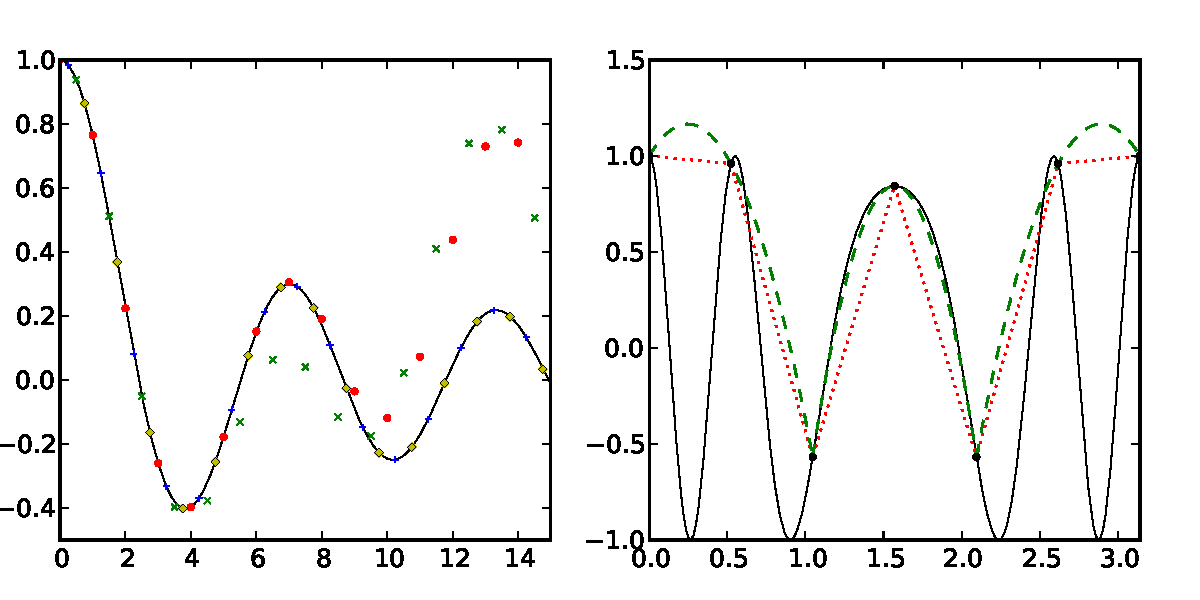
\includegraphics[width=\textwidth]{plots/bessel_int}
  \caption{Links: numerische Lösungen für das Besselintegral
    \eqref{eq:besselint}. Die durchgezogene schwarze Linie markiert
    die analytische Lösung. Blaue Plus-Symbole und gelbe Rauten
    markieren Trapez- bzw. Simpsonregel mit jeweils 20 Stützstellen.
    Rote Punkte und grüne Kreuze markieren dieselben Quadraturformeln,
    aber mit nur 6 Stützstellen. Rechts: in schwarz ist der Integrand
    von \eqref{eq:besselint} für $x=12$ dargestellt. Die schwarzen
    Punkte markieren darauf die 6 Stützstellen, durch die das Integral
    abgeschätzt werden soll. Rot gepunktet sind die linearen
    Näherungen, die in der Trapezregel integriert werden, grün
    gestrichelt die quadratischen Näherungen der zusammengesetzten
    Simpsonregel. Es ist klar, dass diese keine zufriedenstellende
    Auflösung des Integrals liefern können.}
  \label{fig:bessel_int}
\end{figure}

Als Beispiel für die numerische Integration soll uns noch einmal die
Besselfunktion erster Ordnung $J_\nu(x)$ dienen, also die Lösung der
Besselschen Differentialgleichung. Wie man durch Einsetzen in die
Differentialgleichung "`leicht"' sieht, ist $J_0(x)$ gegeben durch das
bestimmte Integral
\begin{equation}
  \label{eq:besselint}
  J_0(x) = \frac{1}{\pi} \int_0^\pi  \cos(x\sin(\tau))\,d\tau,
\end{equation}
das wir numerisch mit Hilfe der zusammengesetzten Trapez- und
Simpsonregel berechnen wollen. Wie Abbildung~\ref{fig:bessel_int}
links zeigt, gelingt dies mit nur 20 Stützpunkten recht
zufriedenstellend, sechs Stützpunkte allerdings ist für beide Regeln
nicht ausreichend. Zum Vergleich: die numerische Lösung der
Differentialgleichung mit dem Verfahren dritter Ordnung benötigt
dreihundert Stützpunkte, liefert aber auch eine Abschätzung der
Funktion an jedem Stützpunkt, während das Integral für jeden Punkt neu
gelöst werden muss.

Der Grund, dass sechs Stützstellen nicht ausreichen, ist im Prinzip
derselbe, wie wir ihn schon bei Abbildung~\ref{fig:num_diff} gesehen
haben: mit nur sechs Stützstellen lassen sich bei höheren $x$ die
Schwingungen nicht mehr auflösen, siehe Abbildung~\ref{fig:bessel_int}
rechts. Dies lässt sich auch durch das Verfahren höherer Ordnung nicht
korrigieren, sondern nur durch eine hinreichend kleine
Schrittweite. In diesem Fall sollte $h \ll 2\pi/x$ bzw. $N \gg x/2$
sein, so dass
\begin{equation}
  \abs{x\left(\sin(\tau + h) - \sin(\tau)\right)} \approx x h
  \abs{cos(\tau)} \ll 2\pi,
\end{equation}
damit der äußere Cosinus ausreichend aufgelöst wird.  Für größere $x$
als im Graphen gezeigt wird also auch $N=20$ nicht ausreichend sein.

\subsection{\keyword{Romberg-Integration}}
\index{Integration>Romberg-}

Ist $f\in C^{2k+2}([a,b])$ und
\begin{equation}
  T_f(h) = h\left(\frac{f(a)}{2} + \sum_{i=1}^{(b-a)/h - 1} f(a + i h) +
    \frac{f(b)}{2}\right) + \O(h^2)
\end{equation}
die (zusammengesetzte) Trapezformel zur Schrittweite $h$, so gilt die
\emph{\keyword{Euler-McLaurin-Summenformel}}
\begin{equation}
  T_f(h) = \int_a^b f(x)\,dx + \sum_{i=1}^k h^{2i}\alpha_i + \O(h^{2k-2})
\end{equation}
mit
\begin{equation}
  \alpha_i = \frac{b_{2i}}{(2i)!}\left(f^{(2i-1)}(b) - f^{(2i-1)}(a)\right).
\end{equation}
$b_{2i}$ bezeichnet dabei die Bernoullizahlen, die $\alpha_i$ hängen also
nicht von $h$ ab. 

In anderen Worten bedeutet das, dass sich der die Trapezregel in einer
Umgebung der 0 wie ein Polynom in $h^2$ verhält!  Damit können wir --
sofern wir die Werte $\alpha_i$ bestimmen können -- durch Auswerten
des Polynoms bei $h=0$, also bei unendlich kleiner Schrittweite, das
gesuchte Integral bis auf einen Fehler der Ordnung $\O(h^{2k-2})$
ausrechnen.

Für $b-a$-periodische $C^\infty$-Funktionen sind offenbar alle
$\alpha_i=0$, daher strebt die Trapezformel $T_f(h)$ für diese
schneller als jede Potenz von $h$ gegen das gesuchte Integral.

Für nichtperiodische Funktionen kann man im allgemeinen die $\alpha_i$
nicht analytisch bestimmen, weil das die Kenntnis hoher Ableitungen
erfordert. Um das gesuchte Polynom $T_f(h)$, und damit die $\alpha_i$,
trotzdem zu bestimmen, berechnet man zunächst $T_{i,0}=T_f(h_i)$ für
paarweise verschiedene Schrittweiten $h_0>h_1>\ldots>h_k>0$, und
bestimmt dann $T_f(h)$ als das interpolierende Polynom durch diese
Punkte. Dann kann man mit Hilfe des Neville-Aitken-Schemas das
interpolierende (Fehler-)Polynom in $h^2$ an der Stelle $0$ auswerten:
\begin{equation}
  \label{eq:richardson}
  T_{i,j} = T_{i+1,j-1} + \frac{T_{i+1,j-1} -
    T_{i,j-1}}{\frac{h_i^2}{h_{i+j}^2} -1}
  \quad\text{für}\; i=0(1)k-j, j=1(1)k.
\end{equation}
Dann gilt $T_{0,k} = T_f(0) + \O(h^{2k+2}) = \int_a^b f(x)\,dx +
\O(h^{2k+2})$. Eine solche Extrapolation von Schrittweiten $h>0$ auf
die Schrittweite Null heißt auch
\emph{\keyword{Richardson-Extrapolation}}.

Wählt man nun $h_i = \frac{b-a}{2^i}$, so vereinfacht sich
\eqref{eq:richardson} zu
\begin{equation}
  T_{ij} = T_{i+1,j-1} + \frac{T_{i+1,j-1} -
    T_{i,j-1}}{4^j - 1} = \frac{4^j T_{i+1,j-1} -
    T_{i,j-1}}{4^j - 1},
\end{equation}
was als \emph{Romberg-Integration} bezeichnet wird. Diese Wahl
der Schrittweiten hat auch den Vorteil, dass die Summe für $h_i$ bei
der Berechnung von $h_{i+1}$ wiederverwendet werden kann:
\begin{equation}
  T_f(h_{i+1}) = \frac{1}{2} T_f(h_i) +
  h_{i+1}\sum_{l=0}^{2^i-1} f\left(a + h_i\left(l
      + \frac{1}{2}\right)\right)
\end{equation}
Da sich der Aufwand für die Berechnung aller $T_f(h_i)$ mit jeder
Stufe verdoppelt, ist der Gesamtaufwand nicht wesentlich größer als
der Aufwand zur Berechnung der niedrigsten Stufe $T_f(h_k)$ alleine,
bei deutlicher Verbesserung der
Fehlerabschätzung. Codebeispiel~\ref{lst:romberg} am Ende des Kapitels
zeigt eine einfache, aber effiziente Implementation des
Rombergverfahrens mit Hilfe von SciPy. Alternativ bietet auch SciPy
selber eine Implementation des Verfahrens,
\scipy{scipy.integrate.romberg(f, a, b)}.

\lstinputlisting[style=floating,firstline=10,
caption={Romberg-Integration von $4(1+x^2)^{-1}$. Das Programm
  berechnet $\pi$ auf 16 Stellen genau.},
label=lst:romberg]{romberg.py}
\afterpage{\clearpage}
  
\subsection{Beispiel: Fehlerintegral}

Als Beispiel für die Romberg-Integration ist das Besselintegral aus
dem vorherigen Abschnitt wenig geeignet, da die zu integrierende
Funktion $b-a$-periodisch und $C^\infty$ ist. Dadurch konvergiert
bereits die einfache Trapezregel schneller als jedes Polynom, und
bereits mit nicht sehr kleinen Schrittweiten erreicht die Trapezregel
Maschinengenauigkeit. Da andererseits die Schrittweite wie beschrieben
hinreichend klein sein muss, bleibt nicht genügend Raum, um durch
Extrapolation noch etwas zu verbessern. 

\begin{figure}
  \centering
  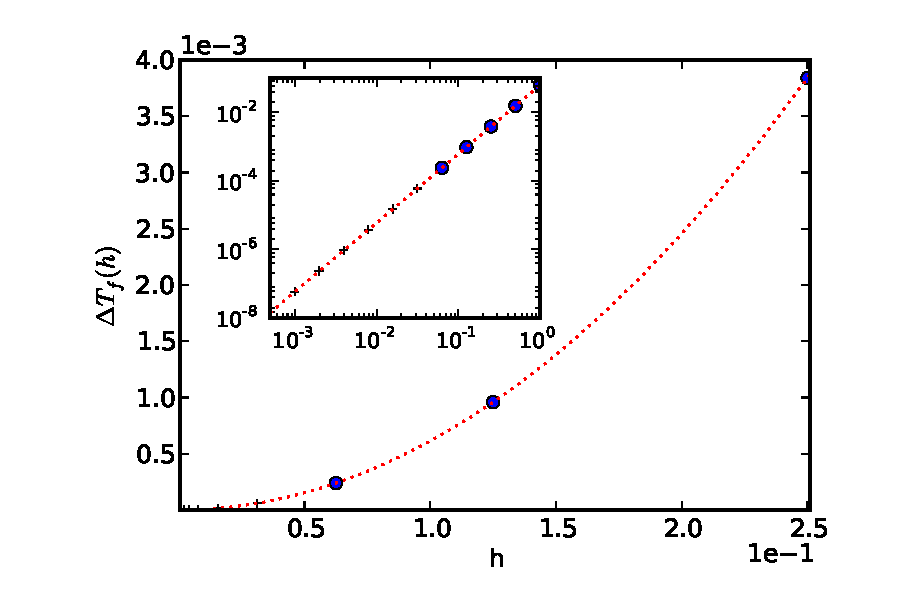
\includegraphics[width=0.75\textwidth]{plots/romberg}
  \caption{Romberg-Integration am Beispiel von $\int_0^1 e^{-x^2}\,dx
    = \sqrt{\pi}\erf(1)/2 =: T_0$. Aufgetragen ist der Fehler $\Delta
    T_f(h) = T_f(h) - T_0$ als Funktion der Schrittweite $h$ (im Einschub
    in doppeltlogarithmischer Skala). Sowohl Kreuze also auch blaue
    Kreise markieren Berechnungen mit der Trapezregel. Durch die mit
    blauen Kreisen markierten Datenpunkte wurde dann das
    interpolierende Polynom bestimmt und rot gestrichelt
    eingezeichnet. Während der beste benutzte Datenpunkt eine
    Genauigkeit von etwa $6\cdot10^{-5}$ erreicht, hat der
    extrapolierte Wert eine Genauigkeit von $3\cdot 10^{-16}$.  }
  \label{fig:romberg}
\end{figure}

Stattdessen wollen wir hier das Fehlerintegral $\int_0^1 e^{-x^2}\,dx
= \sqrt{\pi}\erf(1)/2$ verwenden (siehe Abbildung~\ref{fig:romberg}).
Dabei sind die Randwerte bereits der ersten Ableitung stark
verschieden, so dass $T_f(h)$ tatsächlich polynomielle Form hat und um
die Null herum in einer weiten Umgebung nahezu quadratisch ist. Daher
kann die Extrapolation den Fehler signifikant senken.  Im Beispiel
werden Schrittweiten der Trapezregel von 1 bis $1/16$ betrachtet. Bei
Schrittweite $1/16$ beträgt der Fehler der Trapezregel noch etwa
$6,0\cdot 10^{-5}$, während das Integral durch die Extrapolation von 5
Datenpunkten das Integral bis auf $3,3\cdot 10^{-16}$ korrekt
bestimmt, also Maschinengenauigkeit.

\subsection{\keyword{Gauß-Quadratur}}
\index{Integration>Gauß-Quadratur}

Bis jetzt hatten wir uns vor allem mit äquidistanten oder aber ganz
freien Gittern beschäftigt. Wenn aber die zu integrierende Funktion
analytisch gegeben ist, so können wir die Stützpunkte frei
wählen. Welche Stützpunkte sind dann optimal? Bei der Gauß-Quadratur
suchen wir Stützstellen $x_i$ und dazugehörige Gewichte $\alpha_i$, so
dass für Polynome $f$ mit möglichst hohem Grad noch
\begin{equation}
  \int_{-1}^1 f(x)\, dx = I_n f := \sum_{i=1}^n \alpha_i f(x_i)
\end{equation}
gilt, also dies Polynome exakt integriert werden. Die feste Wahl der
Integralgrenzen $a=-1$ und $b=1$ ist dabei keine Einschränkung, weil
jedes endliche Integral auf diesen Bereich transformiert werden kann:
\begin{equation}
  \int_a^b f(x)\, dx = \frac{(b-a)}{2} \int_{-1}^{1}f\bigl(
  \frac{a+b}{2} + x'\frac{b-a}{2}\bigr)\, dx'.
\end{equation}

Welchen Polynomgrad können wir so erreichen?  Auf der einen Seite
integrieren schon die Newton-Cotes-Formeln mit $n$ Stützstellen
Polynome bis Grad $n-1$ exakt. Auf der anderen Seite ist für das
Polynom $p(x) = \prod_{i=1}^n (x-x_i)^2$ jede Näherung $I_n p = 0$,
während offenbar $\int_{a}^{b} p(x)\,dx>0$. Daher kann es also kein
Verfahren geben, dass alle Polynome bis Grad $2n$ exakt
integriert. Ein Grad darunter, also $2n-1$ ist allerdings möglich, und
wird durch die Gauß-Quadratur erreicht.

Um ein Polynom $2n-1$ Grades eindeutig zu bestimmen, benötigen wir
$2n$ Stützstellen. Da wir aber nur $n$ Stützstellen benutzen wollen,
liegt es nahe, an diesen auch die Ableitungen einzubeziehen, was ein
Spezialfall der Hermite-Interpolation ist. Wie man leicht sieht, ist
\begin{equation}
  p(x) = \sum_{i=1}^n L_i^2(x)\Bigl\{f(x_i)\bigl[1-2L_i'(x_i)(x-x_i)\bigr] +
    f'(x_i)(x-x_i)\Bigr\}
\end{equation}
das gesuchte Polynom $2n-1$-Grades durch die Stützstellen $(x_i,
f(x_i), f'(x_i))$. $L_i$ bezeichnet die Lagrangepolynome aus Gleichung
\eqref{eq:lagrange}. Daraus ergibt sich die \emph{Hermite-Quadratur}
\begin{equation}
  \int_{-1}^1 f(x)\, dx \approx \int_{-1}^1 p(x)\, dx =
  \sum_{i=1}^{n} \alpha_i f(x_i) + \sum_{i=1}^{n} \beta_i f'(x_i)
\end{equation}
mit
\begin{equation}
  \alpha_i = \int_{-1}^1 L_i^2(x)\bigl[1-2L_i'(x_i)(x-x_i)\bigr]\,dx
  \quad\text{und}\quad
  \beta_i = \int_{-1}^1 L_i^2(x)(x-x_i)\, dx.
\end{equation}

\noindent Ziel ist nun, die Lage der Knoten $x_i$ so zu wählen, dass
die Ableitungen, die wir ja im allgemeinen gar nicht kennen, aus der
Näherungen entfallen:
\begin{equation}
  \label{eq:gaussortho}
  0 \stackrel{!}{=} \beta_i = \prod_{k\neq i}\frac{1}{x_i-x_k}
  \int_{-1}^1 L_i(x)\omega(x)\, dx,
\end{equation}
mit $\omega_n(x):=\prod_{i=1}^n(x-x_i)$. Da die $L_i$ eine Basis der
Polynome vom Grad $n-1$ bilden, bedeutet dies, dass $\omega_n$
bezüglich des üblichen Skalarprodukts $(f,\,g) = \int_{-1}^1
f(x)g(x)\,dx$ senkrecht auf dem Raum der Polynome vom Grad $n-1$
stehen muss. Mit $\beta_i=0$ vereinfacht sich außerdem
\begin{equation}
  \alpha_i = \int_{-1}^1 L_i^2(x)\,dx - 2L_i'(x_i)\beta_i
  = \int_{-1}^1 L_i^2(x)\, dx.
\end{equation}

Wir suchen also ein Polynom $\omega_n$ mit Höchstkoeffizient $1$ und
Grad $n$, dass senkrecht auf alles Polynomen vom Grad $n-1$ steht. Die
Nullstellen dieses Polynoms sind dann die gesuchten Stützstellen
$x_i$.  Die Existenz und Eindeutigkeit von $\omega_n$ kann man mit
Hilfe des Gram-Schmidt-Orthogonalisierungserfahrens konstruktiv
zeigen, dass wir später genauer kennenlernen werden. Die Idee ist
dabei, die Basisvektoren $\{1, x, x^2,\ldots\}$ schrittweise so zu
transformieren, dass sie senkrecht zu einanderstehen.

Dies ergibt, bis auf einen Vorfaktor, die
\emph{\keyword{Legendrepolynome}}, die rekursiv zum Beispiel so
berechnet werden können:
\begin{align}
  P_0(x) &= 1\nonumber\\
  P_1(x) &= x\nonumber\\
  P_n(x) &= \frac{1}{n}\Bigl((2n-1)xP_{n-1}(x) -
    (n-1)P_{n-2}(x)\Bigr).
\end{align}
{\samepage Die Nullstellen der ersten dieser Polynome und die
zugehörigen Gewichte sind
\begin{center}
  \renewcommand{\arraystretch}{1.2}
  \begin{tabular}{r|l|l}
    Grad & Nullstelle & Gewicht\\
    \hline\hline
    1    & $x_0=0$         & $\alpha_0=2$\\
    \hline
    2    & $x_{0,1} = \pm \sqrt{\nicefrac{1}{3}}$ &
    $\alpha_{0,1} = 1$ \\
    \hline
    3    & $x_{0,2} =  \pm \sqrt{\nicefrac{3}{5}}$ &
    $\alpha_{0,2}=\nicefrac{5}{9}$\\
    {}   & $x_1 =  0$                             &
    $\alpha_1=\nicefrac{8}{9}$\\
  \end{tabular}
\end{center}}
In SciPy implementiert \scipy{scipy.integrate.fixed_quad(f, a, b,
  n=5)} die Gauß-Quadratur mit den Nullstellen der
Legendrepolynome. \argd{n} gibt dabei die Anzahl der Stützstellen an,
die benutzt werden sollen.

Um andere Gauß-Quadraturen zu entwickeln, kann man gewichtete
Skalarprodukte betrachten. Wir definieren
\begin{equation}
  (f,g)_w := \int_{-1}^1 f(x)g(x)w(x)\, dx
\end{equation}
als das zur Gewichtsfunktion $w(x)>0$ gehörige Skalarprodukt. Dies
ändert unsere Orthogonalitätsbeziehung \eqref{eq:gaussortho} in
\begin{equation}
  0 \stackrel{!}{=} (L_i,\omega)_w = \int_{-1}^1 L_i(x)\omega(x)w(x)\, dx.
\end{equation}
Wenn wir die ursprüngliche Hermite-Interpolation beibehalten wollen,
bedeutet dies, dass wir auch das Zielintegral entsprechend anpassen
müssen, also nun
\begin{equation}
  \int_{-1}^1 f(x) w(x)\, dx \approx \int_{-1}^1 p(x) w(x)\, dx
  \sum_{i=1}^{n} \alpha_i f(x_i) + \sum_{i=1}^{n} \beta_i f'(x_i)
\end{equation}
berechnen mit
\begin{equation}
  \alpha_i = \int_{-1}^1 L_i^2(x)w(x)\, dx.
\end{equation}

Die Legendrepolynome bzw.\ deren Nullstellen gehören also zur
Gewichtsfunktion $w(x)=1$. Die Gewichtsfunktion
$w(x)=\nicefrac{1}{\sqrt{1-x^2}}$ hingegen liefert als Stützstellen
die Nullstellen der Chebyshev-Polynome $T_n(x)$, vergleiche
\eqref{eq:chebyshev}. Die Gewichte sind in diesem Fall sehr einfach,
nämlich $\pi/n$. Um das offene Intervall $(-\infty,\infty)$ zu
betrachten, kann die Gewichtsfunktion $e^{-x^2}$ benutzt werden, zu
der die orthogonalen Polynome die Hermitepolynome sind.

Als letztes soll noch erwähnt werden, dass die Gauß-Quadratur für alle
Gewichtsfunktionen mit steigender Anzahl von Stützstellen gegen das
tatsächliche Integral konvergiert, im Gegensatz zun den
Newton-Cotes-Formeln.

\subsection{Unendliche Integrale und Singularitäten}

\begin{figure}
  \centering
  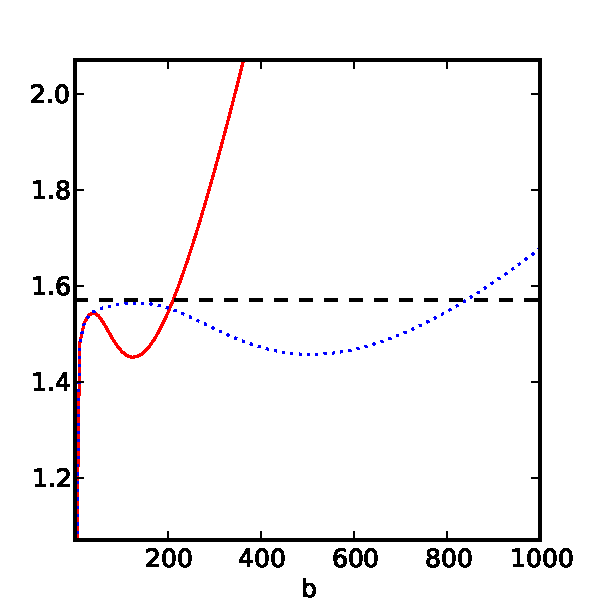
\includegraphics[width=0.5\textwidth]{plots/inf_int}
  \caption{Romberg-Verfahren für das Integral $\int_0^{b}
    \frac{1}{1+x^2}\, dx$, als Funktion von $b$. Die blau gepunktete
    Linie markiert die Ergebnisse des Verfahrens mit 128 Stützstellen,
    die rote durchgezogene Linie mit 32 Stützstellen. Die schwarz
    gestrichelte Linie markiert $\nicefrac{\pi}{2}$, also den
    Grenzwert des Integrals gegen unendlich. Eine Kombination von $b$
    und Anzahl Stützstellen zu finden, die diesen Grenzwert gut
    approximiert, ist also sehr schwierig.}
  \label{fig:inf_int}
\end{figure}

Alle genannten numerischen Integrationsverfahren lösen Integrale mit
Singularitäten nur schlecht. Unendliche Integrationsgrenzen sind, bis
auf die Gauß-Quadratur mit Hermitepolynomen, gar nicht möglich. In
ersterem Falle müssen sehr viele Stützpunkte in der Nähe der
Singularität liegen, im zweiten Fall muss das unendliche Integral
durch ein möglichst großes, endliches Intervall approximiert
werden. Allerdings ist es oft möglich, solche Probleme durch
Variablensubstitution zu umgehen.  So ist zum Beispiel
\begin{equation}
  \int_1^{\infty} \frac{f(x)}{x^2}dx \stackrel{z = \frac{1}{x}}{=}
  \int_0^1 f\left(\frac{1}{z}\right)dz.
\end{equation}
Fällt $f'(x)$ für große $x$ gegen $0$ ab, so dass $f$ gegen eine
Konstante strebt, dann ist die Ableitung von $f(1/z)$ gegen $0$
beschränkt, und die Funktion gut integrierbar. Im Unterschied zum
ursprünglichen Integral ist das neue Integral aber eigentlich und
damit mit den genannten Verfahren einfach zu lösen.

Als Beispiel soll die Berechnung von $\pi/2$ gemäß der Formel
\begin{equation}
  \frac{\pi}{2} = \int_0^{\infty} \frac{1}{1+x^2}\, dx
\end{equation}
dienen. Mit obiger Transformation folgt
\begin{equation}
  \int_0^{\infty} \frac{1}{1+x^2}\, dx
  = \int_0^1 \frac{1}{1+x^2}\, dx +  \int_0^1 \frac{1}{1+z^{-2}}z^{-2}\, dz
  = 2\int_0^1 \frac{1}{1+x^2}\, dx.
\end{equation}
Durch Romberg-Integration auf nur 32 Stützstellen kann der Ausdruck
auf der rechten Seite bis auf 14 Stellen genau ausgewertet
werden.

Abbildung~\ref{fig:inf_int} zeigt hingegen, was bei 32 bzw. 128
Stützstellen geschieht, wenn man stattdessen $\int_0^b
\frac{1}{1+x^2}\, dx$ für große $b$ mit Hilfe des Rombergverfahrens
bestimmt. Das Ergebnis hängt stark von der Integrationsgrenze $b$ ab,
und so ist es praktisch unmöglich, zu sagen, was der tatsächliche Wert
des Integrals für $b \rightarrow \infty$ ist. Durch Anpassen der
Anzahl der Stützpunkte an $b$ und damit Konstanthalten der
Schrittweite lässt sich zwar das Integral stabilisieren, trotzdem
müsste man mehrere Werte von $b$ mit hohen Anzahlen an Stützstellen
ausprobieren, um eine gute Näherung sicherzustellen. Im Beispiel
erreicht keines der beiden Extrema vorne mehr als 3 Stellen
Genauigkeit. Daher sollte man stets lieber versuchen, das Integral
durch Substitutionen auf eine endliche Form zu bringen.

\subsection{Mehrdimensionale Integration, \keyword{Monte-Carlo-Integration}}
\index{Integration>Monte-Carlo-}
\label{sec:mc}

Bis jetzt haben wir uns nur mit eindimensionalen Integralen
beschäftigt. Im Prinzip ist es nicht schwer, die obigen Verfahren auch
auf höhere Dimensionen zu erweitern, etwa die zusammengesetzte 
Mittelpunktsregel auf zwei Dimensionen:
\begin{equation}
  \int_a^b \int_c^d f(x, y)\, dx\, dy \approx
  \frac{(b-a)(d-c)}{NM} \sum_{i=0}^{N-1} \sum_{j=0}^{M-1}
  f\bigl(a + (b-a)\frac{i}{N}, c + (d-c)\frac{j}{N}\bigr).
\end{equation}
Hatte man allerdings bei einer hinreichend glatten Funktion bereits
mit hundert Stützstellen gute Ergebnisse erzielen können, benötigt man
nun etwa $100^2=10,000$ Stützstellen.  Mit steigender Anzahl der
Dimensionen wird dies schnell unmöglich zu handhaben. Für die
sogenannte \emph{Zustandssumme} eines Vielteilchensystems zum
Beispiel, einer zentralen Größe in der statistischen Physik, muss etwa
über allen Koordinaten des Phasenraums integriert werden.  Bei nur
hundert Teilchen entspräche das bereits 600 Dimensionen ($3$
Ortskoordinaten plus $3$ Geschwindigkeiten pro Teilchen). Sollten in
jeder dieser Koordinaten nur 2 Stützpunkte benutzt werden, wären
insgesamt trotzdem über $2^{600}= 4\cdot 10^{180}$ Stützpunkte zu
berücksichtigen! Für diesen exponentiellen Anstieg, der bei
praktischen allen hochdimensionalen Problemen auftritt, hat R.~Bellman
den Begriff "`Curse of dimensionality"' geprägt.

Um solche hochdimensionalen Integrale trotzdem annähern zu können,
kann man die Monte-Carlo-Integration einsetzen. Diese benutzt, dass
\begin{equation}
  \mean{\frac{1}{N} \sum_{i=1}^N f(\xi_i)} = \mean{f}_{V} =
  \int_{x\in V} f(x)\,dx / |V|,
\end{equation}
wobei $\xi_i$ verschiedene Ziehungen einer Zufallsvariablen sind, die
gleichverteilt in $V$ ist. $V$ ist dabei ein endliches Untervolumen
des $\RR^n$, $|V|$ sein Volumen. Daher lässt sich das Integral von $f$
als
\begin{equation}
  \int_{x\in V} f(x)\,dx \approx \frac{|V|}{N} \sum_{i=1}^N f(\xi_i)
\end{equation}
nähern, wobei $\xi_i$ hinreichend gute (Pseudo-)Zufallsvektoren aus
$V$ sein müssen. Wie diese generiert werden, ist Thema des nächsten
Kapitels. Was ist nun der Fehler dieser Näherung? Da die $\xi_i$ gemäß
Konstruktion unabhängig sind, lässt sich der Fehler gut mit Hilfe der
Standardabweichung $\sigma(f)$ abschätzen, und beträgt
$|V|\sigma(f)/\sqrt{N}$. Die Standardabweichung kennen wir im
allgemeinen nicht, können sie aber gemäß~\eqref{eq:varest} als
\begin{equation}
  \sigma^2(x) \approx \frac{1}{N-1} \left[\sum_{i=1}^N f(\xi_i)^2 -
    N\left(\sum_{i=1}^Nf(\xi_i)\right)^2\right]
\end{equation}
zusammen mit der Integration abschätzen.

Als SciPy-Code sieht eine Monte-Carlo-Integration noch einfacher als
die Trapezregel aus. Hier ein Code, der zweidimensional über
$[a,b]\times[c,d]$ integriert:
\begin{lstlisting}
from numpy.random import uniform

def montecarlo(f, a, b, c, d, N):
    volumen = (b-a)*(d-c)
    return volumen*sum(f(uniform(a,b,N), uniform(c,d,N)))/N
\end{lstlisting}

Da die Standardabweichung eine Konstante ist, fällt der Fehler der
Monte-Carlo-Integration im allgemeinen wie $\O(N^{-1/2})$. Im
Vergleich dazu fällt der Fehler der Trapezregel im eindimensionalen
wie $\O(N^{-2})$, sofern $f$ genügend glatt ist. Wenn man bei der
Trapezregel die Anzahl der Stützpunkte verdoppelt, dann muss man bei
der Monte-Carlo-Integration mehr als eine Größenordnung mehr Punkte
aufwenden, um dieselbe Verbesserung in der Genauigkeit zu erreichen!

Bei mehrdimensionalen Integralen sieht die Situation allerdings anders
aus. Bei der Trapezregel mit ingesamt $N$ Stützstellen entfallen pro
Dimension $N^{1/n}$ viele Stützstellen, wenn diese auf einem Würfel
gleichmässig in allen Dimensionen verteilt werden.  Die Genauigkeit
ist damit $\O(N^{-2/n})$.  Ab fünf Dimensionen ist damit die
Monte-Carlo-Integration der Trapezregel überlegen.  Ein anderer Fall,
in dem die Monte-Carlo-Integration der Trapezregel überlegen sein
kann, ist wenn die Funktion $f$ nicht genügend glatt oder nicht einmal
stetig ist.

\subsection{\texorpdfstring{Beispiel: Monte-Carlo-Integration von
    $\pi$}{Beispiel: Quasi-Monte-Carlo-Integration von pi}}

Als Beispiel soll diesmal eine andere Methode zur Bestimmung von
$\pi$ dienen, nämlich die Integration der charakteristischen Funktion
\begin{equation}
  \chi_{D^2}(x, y)=
  \begin{cases}
    1 & \text{falls}\; x^2 + y^2 < 1\\
    0 & \text{sonst}
  \end{cases}
\end{equation}
im Bereich $[-1,1]^2$. Das ergibt dann gerade den Kreisinhalt, also
\begin{equation}
  \int_{x\in[-1,1]}\int_{y\in[-1,1]}\chi_{D^2}(x, y)\,dx\,dy
  = \pi.
\end{equation}

\begin{figure}
  \centering
  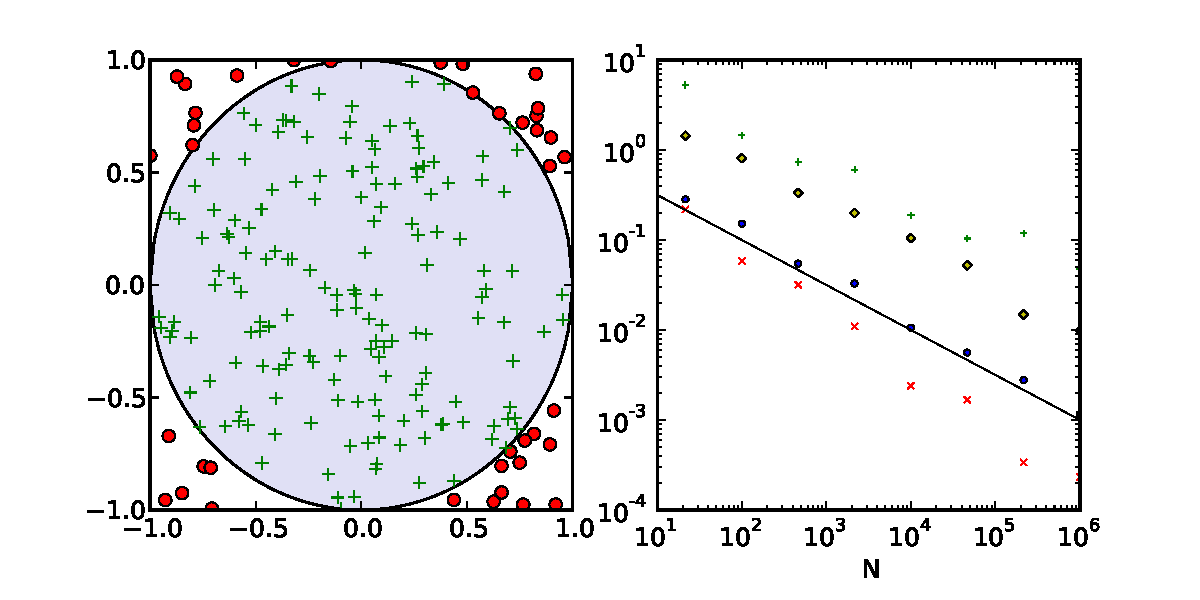
\includegraphics[width=\textwidth]{plots/pi}
  \caption{Links: Illustration der Monte-Carlo-Integration. Die
    Funktion $\chi_{D^2}$ wird über 200 zufällige Punkte (rote Kreise
    und grüne Kreuze) innerhalb $[-1,1]^2$ gemittelt. An den grünen
    Kreuzen ist $\chi_{D^2}=1$, für die roten Punkte ist es
    Null. Rechts: Genauigkeit der Integralnäherungen als Funktion der
    Anzahl der Stützstellen $N$.  Blaue Punkte markieren die mittlere
    Genauigkeit der zweidimensionalen Monte-Carlo-Integration wie
    links skizziert, die roten Kreuze die entsprechende
    Mittelpunktsregel. Gelbe Rauten und grüne Kreuze zeigen die
    Genauigkeiten von Monte-Carlo-Integration und Mittelpunktsregel
    für die 5-Kugel, bei der die Monte-Carlo-Integration schon klar
    überlegen ist. Die durchgezogene Linie entspricht einer Skalierung
    von $N^{-1/2}$, wie man sie für die Monte-Carlo-Integration
    erwartet.}
  \label{fig:pi}
\end{figure}

Abbildung~\ref{fig:pi} skizziert links die Monte-Carlo-Integration von
$\chi_{D^2}$, rechts zeigt sie gemessene Fehler bei
Monte-Carlo-Integration und Mittelpunktsregel. Dabei wurde neben
$\chi_{D^2}$ auch $\chi_{D^5}$ integriert, also das Volumen der
fünfdimensionalen Kugel ($8\pi^2/15$). Der Fehler der
Monte-Carlo-Integration ist als mittlerer Fehler von zwanzig Aufrufen
gemessen, wobei durch die große Anzahl von Abtastungen die
Schwankungen klein sind.

Für das ursprüngliche, zweidimensionale Problem (blaue Punkte und rote
Kreuze) ist die Trapezregel überlegen, auch wenn sie in zwei
Dimensionen nicht die erwartete Skalierung mit $1/N$ erreicht. Das ist
zu erwarten, da die zu integrierende Funktion ja nicht stetig
ist. Auch der nichtmonotone Abstieg der Fehler ist durch die
Unstetigkeit und die Auflösung des Kreisrands bedingt. Beim
fünfdimensionalen Problem aber sieht es wie angekündigt anders aus,
hier ist die Monte-Carlo-Integration besser. Tatsächlich sind nicht
nur die mittleren Abweichungen kleiner als bei der Trapezregel,
sondern es ist sogar sehr unwahrscheinlich, ein ebenso schlechtes
Ergebnis zu erzielen. Für solche Integrale ist also die
Monte-Carlo-Methode in jedem Falle vorzuziehen.

\subsection{\keyword{Quasi-Monte-Carlo-Integration}}
\index{Integration>Quasi-Monte-Carlo-}

Bei der Monte-Carlo-Integration nutzen wir (Pseudo-)Zufallszahlen, um
durch zufällige Abtastung möglichst gut den mittleren Wert der zu
integrierenden Funktion zu bestimmen. Wie wir gesehen haben, sind im
Mehrdimensionalen Zufallszahlen zu diesem Zweck besser geeignet als
ein regelmäßiges Gitter --- das entspräche der ja der
Trapezregel. Aber sind Zufallszahlen optimal?

Tatsächlich nicht, denn etwa Abbildung~\ref{fig:optical_test} links
zeigt, dass Zufallszahlen nicht so homogen verteilt sind, wie man
annehmen würde. Dies ist kein Fehler des betrachteten
Zufallszahlengenerators, sondern ein prinzipielles Problem echter
Zufallssequenzen, die sogenannte \emph{\keyword{Diskrepanz}}. Unsere
Erwartung an eine Reihe von $N$ gleichverteilten Zufallszahlen ist,
dass jedes Intervall $[a,b]\subseteq [0,1]$ von etwa $(b-a)N$
Zufallszahlen getroffen wird. Dies ist aber bei echten Zufallszahlen
erst bei sehr großen $N$ der Fall. Das bedeutet, dass es bei der
Monte-Carlo-Integration immer Bereiche gibt, die von einer echten
Zufallsreihe über- oder unterrepräsentiert werden. Hat aber einer
dieser Bereiche einen großen Anteil am betrachteten Integral, führt
dies zu entsprechenden Fehlern.

\subsubsection{\keyword{Quasizufallszahlen}}

Anstelle von Zufallszahlen benutzt man daher für die
Monte-Carlo-Integration besser \emph{Quasizufallszahlen}, die nicht
mehr wirklich zufällig sind, sondern eine möglichst geringe Diskrepanz
bieten. Ziel ist es also, möglichst alle Bereiche mit genau so vielen
Zahlen abzudecken, wie man nach Gleichverteilung erwarten würde. Ein
Beispiel ist die \emph{\keyword{Halton-Folge}}, die eine Reihe mit
niedriger Diskrepanz im Wertebereich $[0,1]$ ist.

Um die Halton-Folge zu definieren, wählen wir für jede Dimension eine
andere Primzahl $p$ als Basis und schreiben die natürlichen Zahlen in
Basis $p$. Um daraus die gewünschte Zerlegung des Intervalls $[0,1]$
zu erhalten, benutzen wir einfach die Stellen der $p$-Darstellung als
Nachkommastellen, in umgekehrter Reihenfolge:
\begin{center}
  \begin{minipage}[t]{0.49\textwidth}
    \centering
    \begin{tabular}[t]{l|r|l|l}
      $n$ & binär & Stellenumkehr & Ergebnis\\\hline
      1 &   1 & ,1 & \nicefrac{1}{2}\\\hline
      2 &  10 & ,01 & \nicefrac{1}{4}\\
      3 &  11 & ,11 & \nicefrac{3}{4}
    \end{tabular}
  \end{minipage}
  \begin{minipage}[t]{0.49\textwidth}
    \centering
    \begin{tabular}[t]{l|r|l|l}
      $n$ & binär & Stellenumkehr & Ergebnis\\\hline
      4 & 100 & ,001 & \nicefrac{1}{8}\\
      5 & 101 & ,101 & \nicefrac{5}{8}\\
      6 & 110 & ,011 & \nicefrac{3}{8}\\
      7 & 111 & ,111 & \nicefrac{7}{8}
    \end{tabular}
  \end{minipage}
\end{center}
Für $p=3$ ergibt sich analog aus der ternären Darstellung
\begin{center}
  \begin{minipage}[t]{0.49\textwidth}
    \centering
    \begin{tabular}[t]{l|r|l|l}
      $n$ & ternär & Stellenumkehr & Ergebnis\\\hline
      1 &   1 & ,1 & \nicefrac{1}{3}\\
      2 &   2 & ,2 & \nicefrac{2}{3}\\\hline
      3 &  10 & ,01 & \nicefrac{1}{9}\\
      4 &  11 & ,11 & \nicefrac{4}{9}\\
    \end{tabular}
  \end{minipage}
  \begin{minipage}[t]{0.49\textwidth}
    \centering
    \begin{tabular}[t]{l|r|l|l}
      $n$ & ternär & Stellenumkehr & Ergebnis\\\hline
      5 &  12 & ,21 & \nicefrac{7}{9}\\
      6 &  20 & ,02 & \nicefrac{2}{9}\\
      7 &  21 & ,12 & \nicefrac{5}{9}\\
      8 &  22 & ,22 & \nicefrac{8}{9}
    \end{tabular}
  \end{minipage}
\end{center}
Die Umkehrung der Stellen hat den Vorteil, dass die $p^n$-tel
nacheinander möglichst gleichmäßig das Intervall füllen, was ja gerade
einer niedrigen Diskrepanz entspricht. Die sich ergebende Folge heißt
eine \emph{van der Corput-Folge}.

Die mehrdimensionale Halton-Folge ist dann die Folge, die aus der
Verschränkung einer van Corput-Folge für jede Dimension entsteht. Bei
zwei Dimensionen mit Basen 2 und 3 ergibt sich also
\begin{equation}
  \left(\nicefrac{1}{2}, \nicefrac{1}{3}\right),
  \left(\nicefrac{1}{4}, \nicefrac{2}{3}\right),
  \left(\nicefrac{3}{4}, \nicefrac{1}{9}\right),
  \left(\nicefrac{1}{8}, \nicefrac{4}{9}\right),
  \left(\nicefrac{5}{8}, \nicefrac{7}{9}\right),
  \left(\nicefrac{3}{8}, \nicefrac{2}{9}\right),
  \left(\nicefrac{7}{8}, \nicefrac{5}{9}\right),\ldots
\end{equation}

Die folgende Routine berechnet die ersten $N$ Glieder der van der
Corput-Folge zur Basis $p$. Dazu wird solange von den natürlichen
Zahlen $1,2,\ldots,N$ die unterste Stelle abgezogen und mit der
reziproken Potenz auf das Ergebnis addiert, bis alle Stellen von auch
der höchsten Zahl, $N$, bearbeitet wurden:
\begin{lstlisting}
from numpy import *
def vanderCorput(N, p):
    # zu wandelnde Zahlen
    numbers = arange(1,int(N)+1)
    # bitumgekehrtes Ergebnis
    result = zeros(N)
    # Wert der aktuellen, inversen Stelle
    frac = 1.0 / p

    # solange die groesste Zahl noch Stellen hat
    while numbers[-1] > 0:
        # unterste Stelle abschneiden
        digit = numbers % p
        numbers /= p
        # ... und zum Ergebnis hinzufuegen
        result += frac*digit
        frac /= p

    return array(result)
\end{lstlisting}
Um eine Monte-Carlo-Integration mit Quasizufallszahlen durchzuführen,
müssen im Beispielcode zum Abschnitt~\ref{sec:mc} lediglich die
Aufrufe von \lstinline!uniform(a,b,N)! durch
\lstinline!a + (b-a)*vanderCorput(N, p)! ersetzt werden. Üblicherweise
wählt man dabei $p=2$ für die erste Dimension, $p=3$ für die zweite,
und so weiter.

\subsection{\texorpdfstring{Beispiel: Quasi-Monte-Carlo-Integration von $\pi$}{Beispiel: Quasi-Monte-Carlo-Integration von pi}}

\begin{figure}
  \centering
  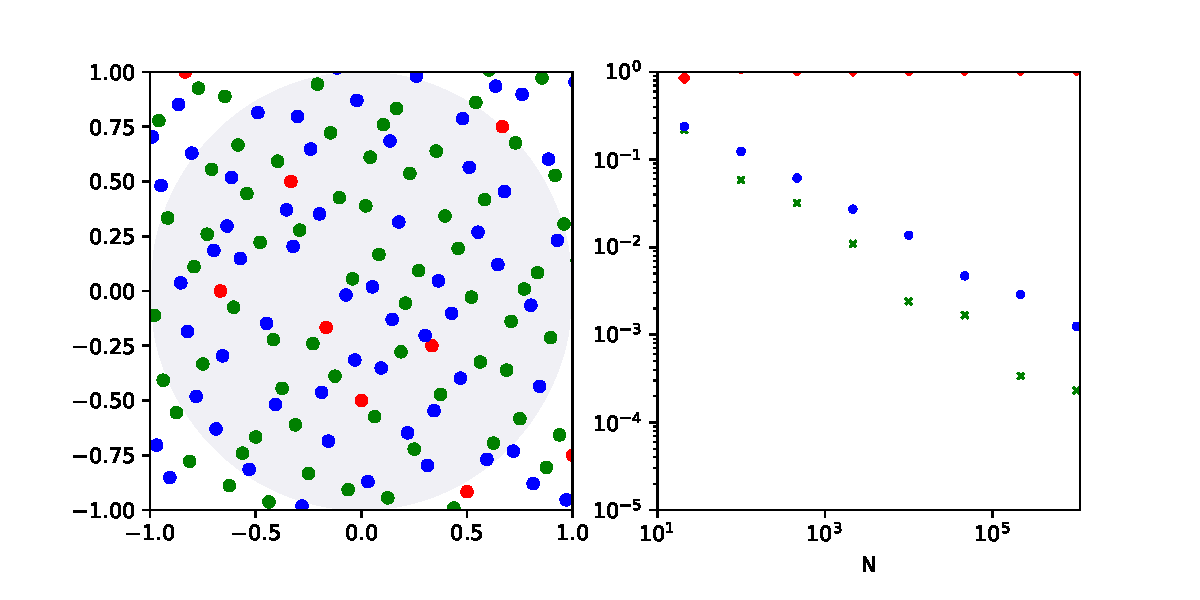
\includegraphics[width=\textwidth]{plots/quasirandom}
  \caption{Quasi-Monte-Carlo-Integration von $\pi$. Wie in
    Abbildung~\ref{fig:pi} sind links die aus der Halton-Folge
    gezogenen Punkte dargestellt, wobei die ersten zehn Punkte rot
    gefärbt sind, die nächsten hundert Punkte blau und die restlichen
    grün. Auf der rechten Seite sind die Ergebnisse der Integration zu
    sehen, wobei blaue Kreise die Monte-Carlo-Integration mit
    Pseudozufallszahlen angeben, grüne Kreuze die Trapezregel und rote
    Diamanten die Quasi-Monte-Carlo-Integration.}
  \label{fig:qmc}
\end{figure}

Abbildung~\ref{fig:qmc} zeigt nochmals die Integration von $\pi$ mit
Hilfe der Monte-Carlo-Integration, allerdings diesmal nicht mit
Pseudozufallszahlen, sondern der Halton-Folge, also
Quasizufallszahlen. Wie man gut sieht, sind die Quasizufallszahlen
scheinbar zufällig, aber sehr viel homogener als echte oder
Pseudozufallszahlen über das Quadrat verteilt, insbesondere auch schon
bei niedrigen Anzahlen von Punkten.  Die Integration mit
Quasizufallszahlen wird kurz als \emph{Quasi}-Monte-Carlo-Integration
bezeichnet, und ist für die unstetige Indikatorfunktion nicht nur der
Monte-Carlo-Integration mit Zufallszahlen überlegen, sondern auch der
Trapezregel.

%%% Local Variables: 
%%% mode: latex
%%% TeX-master: "padc.tex"
%%% TeX-PDF-mode: t
%%% End: 

% Dies ist Teil der Vorlesung Physik auf dem Computer, SS 2012,
% Axel Arnold, Universitaet Stuttgart.
% 
% Dieses Werk ist unter einer Creative Commons-Lizenz vom Typ
% Namensnennung-Weitergabe unter gleichen Bedingungen 3.0 Deutschland
% zugänglich. Um eine Kopie dieser Lizenz einzusehen, konsultieren Sie
% http://creativecommons.org/licenses/by-sa/3.0/de/ oder wenden Sie sich
% schriftlich an Creative Commons, 444 Castro Street, Suite 900, Mountain
% View, California, 94041, USA.

\chapter{\keyword{Zufallszahlen}}
\index{Zufallszahlen>echte}

Im letzten Kapitel wurden für die Monte-Carlo-Integration
Zufallszahlen benötigt. In diesem Kapitel wird besprochen, wie diese
auf dem Computer generiert werden, welche Arten es gibt, und wie die
Qualität einer Zufallsreihe bestimmt werden kann. Außerdem lernen wir
weitere Anwendungen von Zufallszahlen kennen.

Zunächst aber klären wir, was Zufallszahlen im strengen Sinn sind. Wir
betrachten ein Experiment, dass wiederholt voneinander unabhängige
Ergebnisse $x \in M$ liefert.  Dann heißt ein Ergebnis einer solchen
Messung eine \emph{Zufallszahl}. Aufgrund der Konstruktion ist für
jede Zufallszahl $x$ der Erwartungswert gleich und unabhängig von
allen anderen Messungen. Betrachtet wir eine unendliche
Menge von Zufallszahlen, so sind die Zufallszahlen in dieser Menge
stets gleich verteilt, und zwar mit einer Verteilung $P(x)$, die durch
die Art des Experiments bestimmt ist.

Ein solches Experiment wäre zum Beispiel der Wurf eines Würfels, der
Ergebnisse aus $M=\{1,\ldots,6\}$ liefert. Ist dieser Würfel ideal, so
gilt $P(x) =\nicefrac{1}{6}$ für alle $x\in M$. Eine konkrete
Folge von Zufallszahlen wäre dann zum Beispiel
\begin{align*}
&633142563552446623663665614512446522561664446144244634522555 \\
&523121622535453613443366636251342661262345213346341313326554 \\
&221663665263462152654312621424115144626242451444653655341323\ldots
\end{align*}
und mit wachsender Folgenlänge würde der Anteil an Einsen, Zweien und
so weiter gegen jeweils $\nicefrac{1}{6}$ der Gesamtmenge
konvergieren.

Um echte Zufallszahlen bereitzustellen, müsste der Computer
vergleichbar ein (miniaturisiertes) Experiment mit bekannter,
stochastischer Verteilung der Messergebnisse durchführen. Wie Linux
zeigt, ist so etwas durchaus möglich, indem viele verschiedene
Hardwaredaten kombiniert werden, wie etwa Bits aus dem Netzwerkverkehr
oder der Mausposition. Diese Daten werden noch so transformiert, dass
sie gleichverteilte Bytes ergeben, die unter \texttt{/dev/random}
ausgelesen werden können. Wenn nichts weiter angegeben ist, wird auf
dem Computer übrigens üblicherweise von einer Gleichverteilung der
Zufallszahlen ausgegangen, also $P(x) = \nicefrac{1}{\abs{M}}$.

\section{\keyword{Pseudozufallszahlen}}
\index{Zufallszahlen>Pseudo-}

Für physikalische Anwendungen benutzt man allerdings keine echten
Zufallszahlen, sondern sogenannte \emph{Pseudozufallszahlen}. Dies
sind deterministische Zahlenfolgen, die aber "`hinreichend"' zufällig
aussehen; wir werden später sehen, was genau das
heißt. Pseudozufallszahlen haben zwei Vorteile. Zum einen lassen sich
solche Zahlen erheblich schneller berechnen als etwa die echten
Zufallszahlen des Linux-Kernels (um gut einen Faktor 80 auf modernen
Prozessoren), zum zweiten macht dies Computerexperimente exakt
reproduzierbar. Beobachtet man also bei einem Durchlauf ein
ungewöhnliches Verhalten, das man genauer analysieren möchte, kann man
das Experiment exakt wiederholen und dabei zum Beispiel zusätzliche
Messungen vornehmen.

Wie werden solche Pseudozufallszahlen generiert? Für diese Aufgabe
gibt es verschiedene Algorithmen, sogenannte
\emph{\keyword{Zufallszahlengeneratoren}} (engl. \emph{random number
  generator} oder \emph{RNG}). Diese liefern bei jedem Aufruf eine
Zufallszahl, meist eine gleichverteilte Ganzzahl. Die Bandbreite
reicht vom sehr guten, aber aufwändigen Mersenne-Twister bis zu den
einfachen linearen Kongruenzgeneratoren, die wir nun kennenlernen
werden.

Das Hauptmaß für die Güte eines solchen Zufallszahlengenerators ist
seine \emph{Periode}. Denn da jeder Zufallsgenerator einen internen
Zustand hat, der durch $N$ viele Bits dargestellt wird, muss sich nach
höchstens $2^N$ Aufrufen der interne Zustand wiederholen. Da es sich
aber um einen deterministischen Algorithmus handelt, wiederholt sich
die folgende Reihe ab dann exakt. Daher sind alle Generatoren
periodisch. Durch geeignete Wahl des Algorithmus ist die Periode meist
nahe dem theoretischen Maximum, also etwa $2^{32}\approx 4$ Milliarden
bei 32 Bit.

Das hört sich recht viel an, aber bei einer typischen
Molekulardynamiksimulation werden pro Zeitschritt und Teilchen 3
Zufallszahlen benötigt.  Bei zehntausend Teilchen werden damit pro
Schritt 30,000 Zufallszahlen gezogen, und der Generator wiederholt
sich nach weniger als 200,000 Zeitschritten. Da sich die
Teilchenpositionen in dieser Zeit wahrscheinlich schon stark geändert
haben, spielt dies in in der Praxis keine Rolle.  Bei Isingmodellen,
bei denen zufällig Spins auf einem Gitter invertiert werden,
betrachtet man allerdings nicht selten Gitter von einigen Millionen
Spins. In diesem Fall sind bessere Generatoren wesentlich.  Der
Mersenne-Twister-Generator hat zum Beispiel einen internen Zustand von
2,5 Kilobyte und eine Periode von $\approx 10^{6000}$, was für die
meisten Anwendungen ausreichend sein dürfte.

In Python stellt das Modul \texttt{random} verschiedene effiziente und
hochwertige Methoden zur Zufallszahlenberechnung bereit. Die Methode
\scipy{random.randint(a,b)} etwa liefert eine gleichverteilte
Zufallszahl aus dem Interval $[a,b]$; anders als bei \lstinline!range!
etwa ist also auch die obere Grenze
einbegriffen. \scipy{random.unifom(a,b)} liefert analog eine
gleichverteilte Fließkommazahl im Interval
$[a,b]$. \scipy{random.gauss(mu, sigma)} schließlich liefert eine
normalverteilte Fließkommazahl mit Erwartungswert \argd{mu} und
Standardabweichung \argd{sigma}.

NumPy hat ein eigenes \texttt{random}-Modul, das zusätzlich Vektoren
von Zufallszahlen generieren kann, indem einfach neben den Parametern
eine weitere ganze Zahl, die gewünschte Anzahl $N$ von Zufallszahlen,
angeben wird, also zum Beispiel \scipy{numpy.random.normal(mu, sigma,
  N)}. Achtung: anders beim \texttt{random}-Modul von Python ist bei
\scipy{numpy.random.randint(a, b, N)} \argd{b} \emph{nicht}
eingeschlossen!

\subsection{Linearer Kongruenzgenerator}
\index{Kongruenzgenerator>linearer}

Der (lineare) Kongruenzgenerator (LCG) ist der einfachste Typ eines
Zufallszahlengenerators. Der interne Zustand ist dabei lediglich eine
ganze Zahl $x_i$ von $0$ bis $m-1$, die gemäß
\begin{equation}
  x_{i+1} = a x_i + b \bmod m
\end{equation}
in den neuen inneren Zustand $x_{i+1}$ transformiert wird.  Die
eigentliche Zufallszahl sind einige (oder alle) der Bits des Zustands
$x_i$.  $m$, $a$ und $b$ sowie die Menge der für die Zufallszahl
benutzten Bits sind die Konstanten, die den Algorithmus festlegen,
$x_0$ der Startwert oder \emph{\keyword{Seed}}.  Die Konstanten $m$,
$a$ und $b$ sollten keinesfalls einfach zufällig gewählt werden, da
Knuth gezeigt hat, dass nur unter gewissen Bedingungen die Periode
eines solchen Generators tatsächlich $m$ ist~\cite{knuth81b}.  Bei
zufälliger Wahl der Konstanten wird die Periode meist sehr viel kürzer
sein.

Der Zufallsgenerator \texttt{rand48} der POSIX-C-Bibliothek ist ein
Beispiel eines LCGs.  Er benutzt einen Modul von $m=2^{48}$,
$a=25,214,903,917$ und $b=11$.  Als Zufallszahlen werden dann die
obersten 31 Bits von $x_i$ benutzt, also die Bits 17 bis 47.  Ältere
Versionen der Standard-C-Bibliothek benutzten für die Funktion
\texttt{rand} $m=2^{32}$, $a=1,103,515,245$ und $b=12,345$, wovon die
unteren 31 Bit als Zufallszahl genutzt werden.

Die Wahl von $m=2^{48}$ bzw. $m=2^{32}$ hat den einfachen Grund, dass
sich sehr einfach modulo $m=2^b$ rechnen lässt -- man berücksichtigt
einfach nur die ersten $b-1$ Bits und ignoriert alle höheren. Denn
\begin{equation}
  \label{eq:lcgmod}
  \left(\sum_{i=0}^\infty b_i 2^i\right) \bmod 2^b =
  \sum_{i=0}^\infty b_i \underbrace{\left(  2^i \bmod 2^b \right)}_{=
      0\,\text{für}\; i\ge b} \bmod 2^b = \sum_{i=0}^{b-1} b_i 2^i.
\end{equation}
Daher kann der klassische \texttt{rand} in C etwa wie folgt
implementiert werden:
\begin{lstlisting}[language=C]
unsigned int state = 1;

void rand_seed(unsigned int seed)
{
  state = seed;
}

unsigned int rand()
{
  const unsigned int a = 1103515245, b = 12345;
  state = a * state + b;
  return state & ((1u<<31) - 1);
}
\end{lstlisting}
Die Funktion \lstinline!seed! dient zum Setzen des internen Zustands,
also $x_0$, \lstinline!rand! liefert dann bei jedem Aufruf eine neue
Zufallszahl.

Dass die Modulo-Operation für eine Zweierpotenz als Modul ein
einfaches Abschneiden der hohen Bits ist, hat allerdings auch einen
gewissen Nachteil.  Die ersten $k$ Bits der Zufallszahl bleiben beim
Abschneiden aller Bits $k+1,\ldots$ übrig.  Das bedeutet, dass diese
anscheinend von einem Generator mit kürzerer Periode $2^{k+1}$
generiert werden.  Insbesondere wechselt das unterste Bit mit jedem
Schritt seinen Wert oder ist konstant.  Dies ist der Grund, warum
\texttt{rand48} die untersten 17 Bit verwirft.

Dieses Problem lässt sich umgehen, in dem der Modul als Primzahl
gewählt wird. In diesem Fall kann $b=0$ gewählt werden, so dass
\begin{equation}
  x_{i+1} = a x_i = a^i x_0 \bmod m,
\end{equation}
wobei offenbar $x_0\neq 0$ sein muss. Wenn $a$ als eine primitive
Einheitswurzel des endlichen Körpers $\FF_m$ gewählt wird, dann
durchläuft diese Reihe einmal alle Elemente außer der Null. Daher hat
ein solcher Generator eine Periode von $m-1$.

$m$ wird meist als Mersennesche Primzahl, also von der Form $m=2^b -
1$, gewählt, wobei $b$ etwa so groß wie die Bitlänge des internen
Zustands ist. Dadurch ist die Periode des Generators nahezu maximal.
Die Implementation ist allerdings etwas schwieriger, weil jetzt die
oberen Bits nicht einfach abgeschnitten werden können. Nach Park und
Miller ist ein Beispiel eines solchen Generators $m=2^{31}-1$ und
$a=16807$, der auch als \texttt{MINSTD} bezeichnet wird und wie folgt
implementiert werden kann:
\begin{lstlisting}[language=C]
int state = 1;

void minstd_seed(unsigned int seed)
{
  state = seed;
}

unsigned int minstd()
{
  const int m = (1u << 31) - 1, a = 16807;
  state = ((long int)state)*a % m;
  return state;
}
\end{lstlisting}
Die Typumwandlung in \lstinline!long int! stellt dabei sicher, dass
das Produkt der beiden 32-Bit-Zahlen in 64-Bit-Arithmetik gerechnet
wird, so dass keine Stellen verloren gehen.

\subsection{Verzögerter Fibonaccigenerator}
\index{Fibonaccigenerator}
\index{Fibonaccigenerator>verzögerter}

Um eine längere Periode zu erzielen, könnte man im Prinzip zu immer
größeren Moduln $m$ übergehen. Allerdings wird es immer schwieriger,
entsprechende Konstanten zu bestimmen, und auch das Rechnung mit
Zahlen großer Bitlänge ist aufwändiger. Eine einfache Alternative
sind \emph{verzögerte Fibonaccigeneratoren}, die ähnlich wie ein LCG
funktionieren, aber mehrere vorherige Werte benutzen:
\begin{equation}
  x_n = x_{n-a} + x_{n-b} \bmod m,
\end{equation}
wobei diesmal $m$ beliebig ist und im allgemeinen einfach als die
Bittiefe des Rechners gewählt wird. Anstelle der Addition kann auch
die bitweise Addition modulo 2 benutzt werden.  Diese
Exklusiv-Oder-Operation war früher schneller als eine Addition und
wurde daher gern benutzt, bringt sonst allerdings eher Nachteile.  Der
interne Status des Zufallszahlengenerators besteht in diesem Fall aus
$\max(a,b)$ vielen $x_i$, die meist in einem
\emph{\keyword{Ringspeicher}} gespeichert werden.  Um diesen zu Anfang
zu füllen, benutzt man üblicherweise einen LCG, der nur einen
Startwert braucht.

Im Fall $a=b=1$ spricht man von einem Fibonaccigenerator, $a$ und $b$
sind ansonsten die Verzögerungen. Der Name stammt von den
Fibonaccizahlen, die ja der analogen Rekursion $x_n = x_{n-1} +
x_{n-2}$ genügen. Der Fibonaccigenerator selber, also $a=b=1$, ist
nicht sehr geeignet, gerade für den in der Physik häufigen Fall von
Dreierblöcken zeigt er unerwünschte Korrelationen.

Anders sieht es bei den verzögerten Fibonaccigeneratoren aus. Sofern
\begin{equation}
  x^a + x^b + 1
\end{equation}
ein primitives Polynom modulo zwei ist, also nicht faktorisierbar, hat
der verzögerte Fibonaccigenerator eine Periodenlänge von mindestens
$2^a-1$. Um einen 32-Bit-LCG an Periodenlänge zu übertreffen,
sind also wenigstens 32 Registerplätze im Ringspeicher nötig. Stoll
und Kirkpatrick geben als Parameter $a=250$, $b=103$ an, eine andere
mögliche Kombination ist $a=521$, $b=168$.

\begin{figure}
  \centering
  \begin{tikzpicture}[thick, x=0.95\textwidth,y=\baselineskip]
    \newcommand{\mycount}{10}%
    \newcommand{\myfirst}{21}%
    \newcommand{\mysecond}{24}%
    \pgfmathsetmacro{\mywidth}{1.0/\mycount}
    
    \draw (1.3*\mywidth, 2) node[anchor=west] {$p = 1$} ;
    \draw[very thick, ->]
    (1.5*\mywidth, 1.5) --
    (1.5*\mywidth, 1) ;

    \draw (4.3*\mywidth, 2) node[anchor=west] {$p + 10 - 7 \bmod 10 = 4$} ;
    \draw[very thick, ->]
    (4.5*\mywidth, 1.5) --
    (4.5*\mywidth, 1) ;

    \draw (2.3*\mywidth, -5) node[anchor=west] {$p' = 2$} ;
    \draw[very thick, ->]
    (2.5*\mywidth, -4.5) --
    (2.5*\mywidth, -4) ;

    \pgfmathsetmacro{\last}{\myfirst + \mycount-1}%
    \foreach \idx in {\myfirst,...,\last} {
      \pgfmathsetmacro{\x}{mod(\idx - 20 + \mycount,
        \mycount)*\mywidth}
      \ifthenelse{\equal{\idx}{\myfirst}}{
        \draw[fill=green!50!white] (\x,0) rectangle +(\mywidth, 1);
      }{}
      \ifthenelse{\equal{\idx}{\mysecond}}{
        \draw[fill=blue!50!white] (\x,0) rectangle +(\mywidth, 1);
      }{}
      \draw (\x,0) rectangle +(\mywidth, 1);
      \draw (\x + 0.5*\mywidth, 0.5) node {$x_{\idx}$};
    }

    \draw (2.5*\mywidth, -1.5) node {$x_{n} = x_{n-10} + x_{n-7}$} ;
    \draw[very thick, dotted, ->]
    (1.5*\mywidth, 0) --
    (1.5*\mywidth, -0.5) --
    (2.5*\mywidth, -0.5) --
    (2.5*\mywidth, -1) ;
    \draw[very thick, dotted, ->]
    (4.5*\mywidth, 0) --
    (4.5*\mywidth, -0.5) --
    (3.5*\mywidth, -0.5) --
    (3.5*\mywidth, -1) ;
    \draw[very thick, dotted, ->] (1.5*\mywidth, -2) -- (1.5*\mywidth, -3) ;

    \renewcommand{\myfirst}{22}%
    \renewcommand{\mysecond}{25}%
    \newcommand{\mylast}{31}%
    \pgfmathsetmacro{\last}{\myfirst + \mycount-1}%
    \foreach \idx in {\myfirst,...,\last} {
      \pgfmathsetmacro{\x}{mod(\idx - 20 + \mycount, \mycount)*\mywidth}
      \ifthenelse{\equal{\idx}{\mylast}}{
        \draw[fill=red!50!white] (\x,-4) rectangle +(\mywidth, 1);
      }{}
      \ifthenelse{\equal{\idx}{\myfirst}}{
        \draw[fill=green!20!white] (\x,-4) rectangle +(\mywidth, 1);
      }{}
      \ifthenelse{\equal{\idx}{\mysecond}}{
        \draw[fill=blue!20!white] (\x,-4) rectangle +(\mywidth, 1);
      }{}
      \draw (\x,-4) rectangle +(\mywidth, 1);
      \draw (\x + 0.5*\mywidth, -3.5) node {$x_{\idx}$};
    }
  \end{tikzpicture}
  
  \caption{Illustration eines Ringspeichers für $b=10$ Werte. $p$ gibt
    die aktuelle Position des ältesten Elements im Ringspeicher an, im
    Beispiel steht an Stelle $p=1$ der Wert $x_{21}$. Das neueste
    Element ist $x_{30}$, daher wollen wir $x_{31}=x_{21} + x_{24}$
    berechnen. $x_{21}$ befindet sich gerade an der Stelle $p$,
    $x_{24}$ dementsprechend $10-7 = 3$ Positionen weiter rechts,
    wobei Positionen jenseits des rechten Randes links wieder
    hereinlaufen. Im nächsten Schritt ist dann $p=2$, und das zweite
    Element an der Stelle 4. Die Folgenwerte sind also wie auf einem
    Ring gespeichert.}
  \label{fig:ringspeicher}
\end{figure}

In Code sieht ein einfacher verzögerter Fibonaccigenerator so aus:
\begin{lstlisting}[language=C]
  /* Position des am weitesten verzoegerten Beitrags x_{n-250}
     Dieser wird im Ringspeicher durch den neuen Wert ersetzt,
     da nicht mehr gebraucht */
  int position = 0;
  // Der Ringspeicher
  unsigned int state[250];

  void r250_seed(unsigned int seed) {
    // minstd zur Initialisierung
    minstd_seed(seed);
    for (int i = 0; i < 250; ++i)
      state[i] = minstd();
    position = 0;
  }

  unsigned int r250() {
    const unsigned int m = (1u << 31) - 1;
    unsigned int newval =
      (state[position] + state[(position + 250 - 103) % 250]) % m;
    state[position] = newval;
    // Ringspeicher weiterschieben
    position = (position + 1) % 250;
    return newval;
  }
}
\end{lstlisting}
Abbildung~\ref{fig:ringspeicher} illustriert dabei die Funktion und
Indizierung des Ringspeichers.

\section{Andere Verteilungen}

Die bisher besprochenen Zufallszahlengeneratoren liefern stets ganze
Zahlen in einem gewissen Intervall, \texttt{rand48} zum Beispiel
im Intervall $[0,2^{31}-1]$, \texttt{MINSTD} im Intervall
$[1,2^{31}-1]$. Um daraus gleichverteilte Ganzzahlverteilungen in
beliebigen Intervallen zu erzeugen, kann man die Zufallszahl einfach
skalieren. Ist also $\xi$ eine Zufallszahl, die gleichverteilt aus
$[a,b]$ gezogen wird, so ist
\begin{equation}
  \xi' = \frac{\xi - a}{b-a}
\end{equation}
gleichverteilt in $[0,1]$ und umgekehrt
\begin{equation}
  \xi'' = a' + \frac{(b'-a')(\xi - a)}{b-a}
\end{equation}
gleichverteilt in $[a',b']$. Dabei muß bei Ganzzahlarithmetik zuerst
multipliziert und dann dividiert werden, da $\xi' \le 1$. Zusätzlich
ist $b$ meist knapp an der Bitlänge der Architektur, daher muss das
Produkt mit doppelter Bitzahl berechnet werden. Da die Prozessoren,
die zum wissenschaftlichen Rechen benutzt werden, meist auch sehr
schnell Fließkommazahlen verarbeiten, kann alternativ auch $\xi'$ in
in Fließkommadarstellung berechnet werden und daraus $\xi''$. Soll
$\xi''$ ganzzahlig sein, kann es dabei einfach gerundet werden. Diesen
Weg benutzt zum Beispiel Python. Auf diese Weise können natürlich auch
(pseudo-)zufällige gleichverteilte Fließkommazahlen erzeugt werden,
insbesondere \emph{Standardzufallszahlen}\index{Standardzufallszahl},
also Fließkommazahlen im Bereich $[0,1]$.

Wie aber können nun etwa normalverteilte Zufallszahlen erzeugt werden?
Hierfür lernen wir nun mehrere Verfahren kennen, die
Standardzufallszahlen in im Prinzip beliebige andere Verteilungen
umwandeln.

\subsection{\keyword{Verwerfungsmethode}}
\index{Rejection sampling}

Angenommen, wir wollen Zufallsvektoren gleichverteilt aus einer
Kreisscheibe vom Radius $1$ ziehen, d.~h.~, wir wollen Zufallsvektoren
$p=(x,y)$ ziehen, die gemäß der Dichte
\begin{equation}
  \rho(x, y) = \begin{cases}
    \nicefrac{1}{\pi} & \text{für}\; x^2+y^2\le 1\\
    0     & \text{sonst}
  \end{cases}
\end{equation}
verteilt sind.  Abbildung~\ref{fig:pi} links zeigt, wie man dies
bewerkstelligen könnte: man zieht zunächst zwei unabhängig
gleichverteilte Zufallszahlen auf $[-1,1]$ und interpretiert diese als
Koordinaten $p = (x, y)$. Liegt $p$ in der Kreisscheibe, akzeptieren
wir dies als unseren Zufallsvektor, ansonsten versuchen wir es einfach
erneut. Da die Wahrscheinlichkeit, gezogen zu werden, für alle
Kreisscheibenpunkte gleich ist, sind die zurückgelieferten $p$
gleichverteilt. Als Code sieht dies so aus:
\begin{lstlisting}
from numpy.random import uniform

def kreisscheibe():
    while True:
        x = uniform(-1, 1)
        y = uniform(-1, 1)
        if x**2 + y**2 <= 1:
            return (x, y)
\end{lstlisting}
Da wir im Mittel nur $1-\pi/4$ der gezogenen Punkte benutzen, brauchen
wir $\nicefrac{4}{(4-\pi)}$ mal mehr Zufallszahlen, als wir als
Koordinaten der Punkte zurückliefern. Im Falle des Kreises ist der
Verlust nicht sehr hoch, aber ist die zulässige Struktur kleiner,
können sehr viele Zufallszahlen zurückgewiesen werden, und die
Verwerfungsmethode wird ineffizient.

\begin{figure}
  \centering
  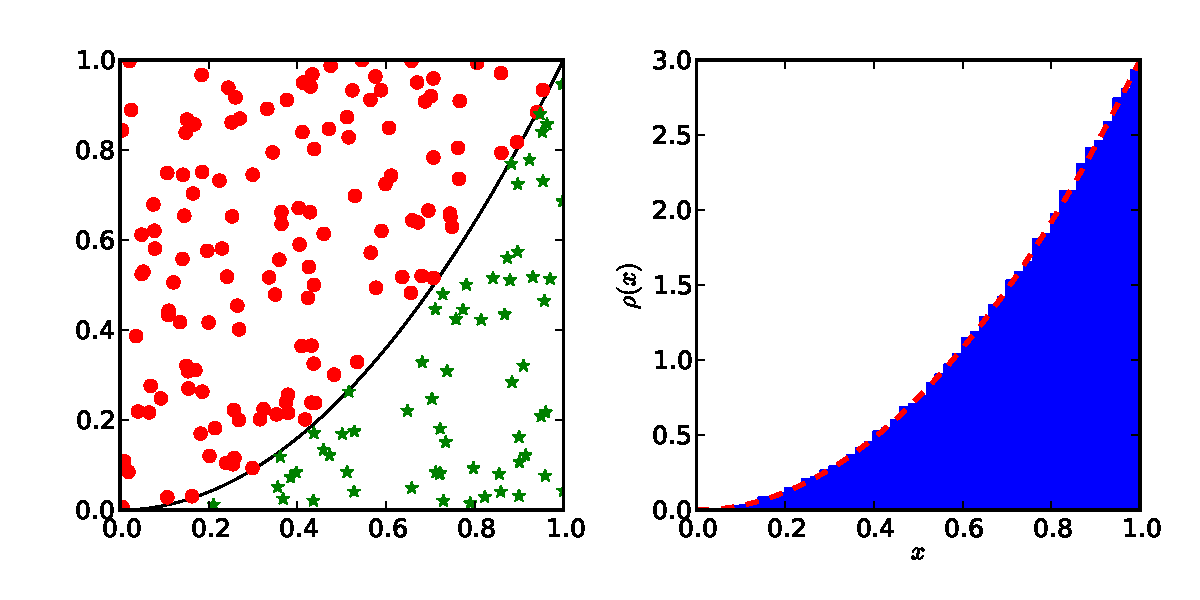
\includegraphics[width=\textwidth]{plots/rejection}
  \caption{Verwerfungsmethode zur unnormierten Verteilung
    $\rho(x)=x^2$ für $0\le x \le 1$. Links sind einige gezogene
    Punkte eingezeichnet, von denen die grünen Sterne akzeptiert
    wurden, die roten Kreise abgelehnt. Der schwarze Strich stellt
    $\rho(x)$ dar. Rechts sind die beobachteten Häufigkeiten der
    Punkte als Balken dargestellt. Diese stimmen gut mit der
    normierten Dichte $3x^2$ überein, die rot gestrichelt
    eingezeichnet ist. Hier werden im Schnitt etwa drei Zufallszahlen
    pro Aufruf der Verwerfungsmethode benötigt.}
  \label{fig:rejection}
\end{figure}

Im Falle der Kreisscheibe war die Dichte $\rho(x, y)$ der gesuchten
Verteilung sehr einfach, nämlich entweder $0$ oder $1/\pi$. Die
Verwerfungsmethode lässt sich aber auch bei komplizierteren $\rho$
anwenden. Wir betrachten nun eine Dichte $\rho:\RR^n\to [0,1]$, so
dass $\rho$ außerhalb $[0,1]^n$ Null ist. Dann müssen die Punkte $p$
mit relativen Wahrscheinlichkeiten $\rho(p)$ gezogen werden. Das lässt
sich einfach bewerkstelligen, indem wir zunächst einen Punkt $p$ durch
Ziehen von $n$ Standardzufallsvariablen gleichverteilt in $[0,1]^n$
bestimmen. Wir ziehen nun eine weitere Standardzufallszahl $u$ und
akzeptieren $p$ nur dann, wenn $u\le\rho(p)$. Die Wahrscheinlichkeit,
$p$ tatsächlich zu ziehen, ist dann
\begin{equation}
  P(u \le\rho(p)) = \rho(p).
\end{equation}

Die korrekte Wahrscheinlichkeit für einen Punkt $p$ im Würfel ist die
infinitesimale Dichte $\rho(p)\,dx^n$. Da der Normierungsfaktor $dx^n$
für alle $p$ gleich ist, können wir diesen vernachlässigen, da die
relativen Wahrscheinlichkeiten auf $[0,1]^n$ trotzdem korrekt
sind. Das bedeutet auch, dass die Eingabe-"`Dichte"' $\rho(p)$ gar nicht
normiert sein muss --- die Verwerfungsmethode liefert stets
Ergebnisse, die gemäß der normierten Dichte
\begin{equation}
  \tilde\rho(p) := \rho(p) / \int_{[0,1]^n} \rho(q)\,dq^n
\end{equation}
verteilt sind. Damit können auch Dichten behandelt werden, die nicht
in $[0,1]$ liegen, so lange sie beschränkt sind, denn man kann in
diesem Fall
\begin{equation}
  \rho'(p) = \frac{\rho(p) + \min_{p\in [0,1]^n} \rho(p)}{
    \max_{p\in [0,1]^n} \rho(p) - \min_{p\in [0,1]^n} \rho(p)} \in [0,1]
\end{equation}
betrachten. Die Normierungseigenschaft ist auch sehr günstig, wenn die
Normierungskonstante nicht einfach bestimmt werden kann, etwa bei sehr
hochdimensionalen Räumen. Dies ist die Grundlage des
Metropolissampling, dass eine zentrale Rolle in der numerischen
statistischen Physik spielt. Abbildung~\ref{fig:rejection} illustriert
die Verwerfungsmethode und ihre Normierungseigenschaft.

Im Falle der Kreisscheibe hatten wir übrigens auch von der
Normierungseigenschaft Gebrauch gemacht, denn eigentlich ist $\rho(p)$
Null außerhalb der Kreisscheibe und $\nicefrac{1}{\pi}$ innerhalb. Da
wir aber die Punkte innerhalb automatisch akzeptiert haben, haben wir
formal ein $\rho'$ betrachtet mit $\rho'(p) = 1$ auf der
Kreisscheibe. Dank der Normierungseigenschaft haben wir damit trotzdem
die korrekte Verteilung erzeugt.

Als Python-Code sieht die allgemeinere Verwerfungsmethode nicht
wesentlich schwieriger aus:
\begin{lstlisting}
from numpy.random import uniform

def verwerfungsmethode(rho, n):
    while True:
        p = uniform(0, 1, n)
        u = uniform(0, 1)
        if u < rho(p):
            return p
\end{lstlisting}
\argd{rho} muss dabei eine Pythonfunktion sein, die als einziges
Argument ein $n$-dimensionales Numpy-Array akzeptiert.

Die Verwerfungsmethode kann so erweitert werden, dass die benutzten
Zufallszahlen  nicht gleichverteilt sind, sondern etwa
normalverteilt. Das erlaubt, die Verwerfungsmethode auch bei über dem
gesamten $\RR^n$ nichtverschwindenden Dichten zu benutzen. Siehe
hierzu zum Beispiel \textcite{knuth81b}. Wie man solche
normalverteilten Zufallszahlen erzeugt, lernen wir nun kennen.

\subsection{\keyword{Inversionsmethode}}

Wegen der Beschränkung auf einen Würfel können wir die
Verwerfungsmethode nicht benutzen, um zum Beispiel normalverteilte
Zufallszahlen aus gleichverteilten zu generieren. Wir benötigen also
noch eine andere Methode, um auch unbeschränkte Verteilungen erzeugen
zu können. Hier bietet sich die Inversionsmethode an.

Sei $\rho:\RR\to \RR$ eine normierte Wahrscheinlichkeitsdichte, zu der
wir passend Zufallszahlen ziehen wollen. Dann definieren wir die
Verteilungsfunktion zu $\rho$ als
\begin{equation}
  F_\rho(x) := P(u_\rho \le x) = \int_{-\infty}^{x} \rho(x')\, dx',
\end{equation}
wobei $u_\rho$ eine $\rho$-verteilte Zufallszahl ist.  $F_\rho(x)$
gibt also die Wahrscheinlichkeit an, einen Wert kleiner als $x$ zu
beobachten, und bildet daher die reelle Achse monoton wachsend in das
Intervall $[0,1]$ ab. Das $p$-Quantil ist nun die Umkehrung
$F_\rho^{-1}(p)$, also diejenige Grenze $x$, bei der ein gezogener
Wert mit Wahrscheinlichkeit $p$ kleiner als $x$ ist. Es gilt also
\begin{equation}
  F_\rho\left(F_\rho^{-1}(p)\right) = p.
\end{equation}

$F_\rho^{-1}(u)$ ist eine $\rho$-verteilte Zufallsvariable, wenn $u$
eine Standardzufallszahl ist, also gleichverteilt auf $[0,1]$. Denn
\begin{equation}
  P(F_\rho^{-1}(u) \le x) = P(u \le F_\rho(x)) = F_\rho(x).
\end{equation}
Sofern also die Quantilfunktion einfach zu invertieren ist, lassen
sich so sehr bequem Zufallszahlen erzeugen, indem $F_\rho^{-1}$ auf
Standardzufallszahlen angewendet wird.

\subsubsection{\keyword{Box-Muller-Verfahren}}

\begin{figure}
  \centering
  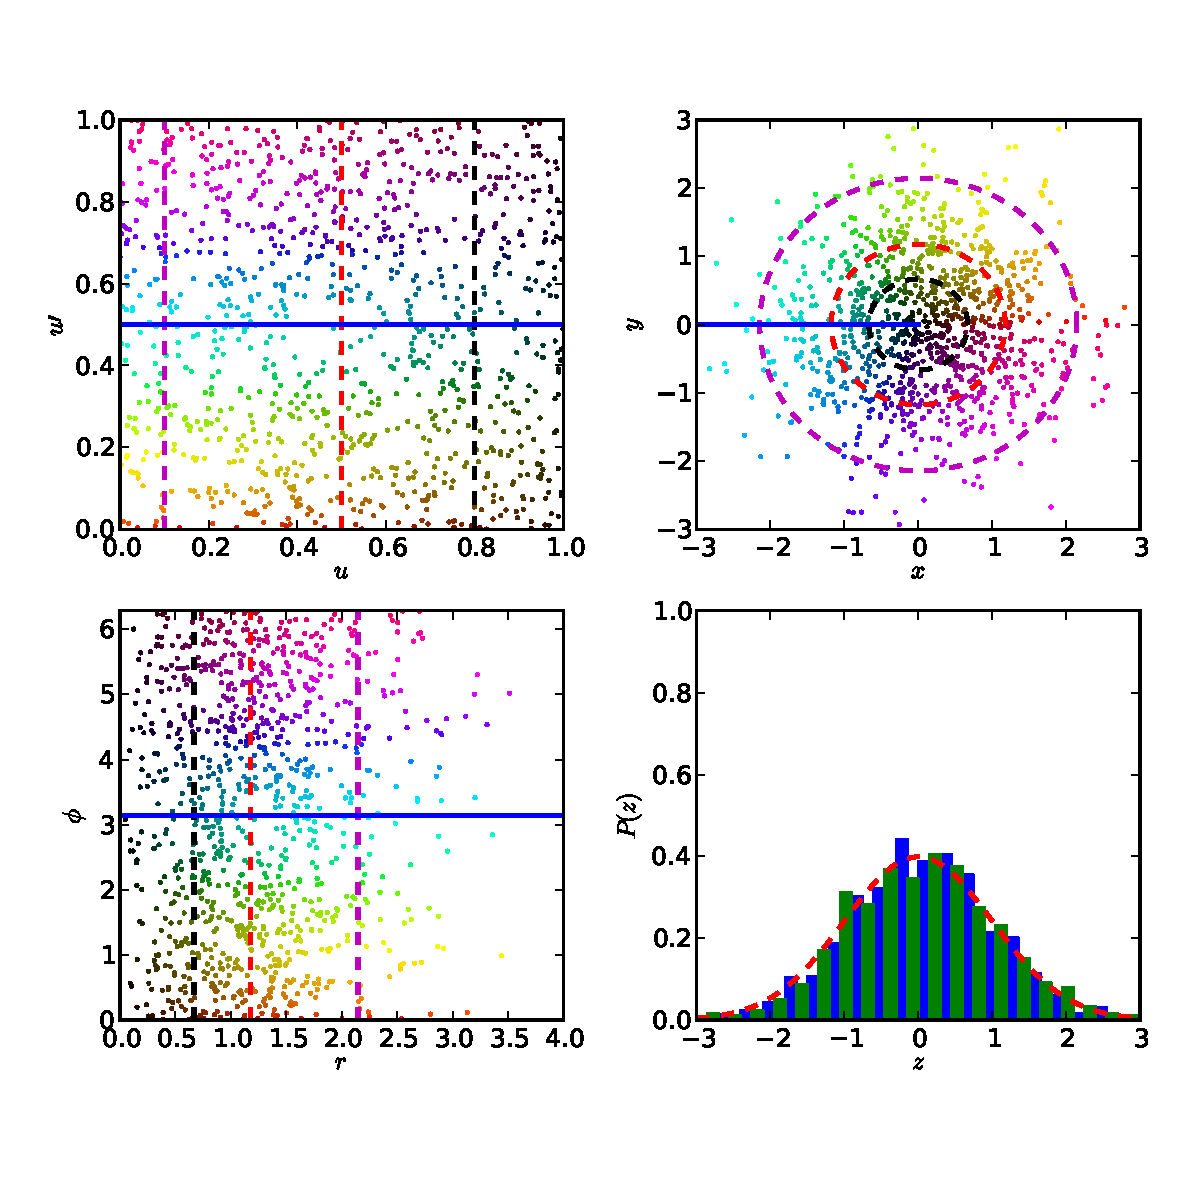
\includegraphics[width=\textwidth]{plots/inversion}
  \caption{Illustration des Box-Muller-Verfahrens zur Erzeugung von
    normalverteilten Zufallszahlen. Die Punkte werden zunächst
    gleichverteilt auf $[0,1]^2$ erzeugt (links oben), dann
    gemäß \eqref{eq:expquantil} auf das Gebiet
    $[0,\infty)\times[0,2\pi]$ transformiert (links unten), und
    schließlich in kartesische Koordinaten (rechts oben). Die Punkte
    sind in allen drei Graphen stets gleich gefärbt, und zwar mit
    wechselnder Farbe im Winkel und sinkender Intensität nach
    außen. Rechts unten sind die gemessenen Verteilungen von $x$ und
    $y$ sowie die erwartete Gaußverteilung gezeigt.}
  \label{fig:boxmuller}
\end{figure}

Mit Hilfe der Inversionsmethode können wir nun auch normalverteilte
Zufallszahlen erzeugen. Allerdings nicht auf direktem Wege, da das
Integral der Gaußfunktion, die Fehlerfunktion, nicht einfach
analytisch zu invertieren ist. Box und Muller gehen daher ähnlich wie
bei der Bestimmung des uneigentlichen Integrals von $e^{-x^2}$ vor
und weichen auf zwei Dimensionen aus.

Wir betrachten also einen Zufallsvektor $(x, y)$ mit Dichte $\rho(x,
y) = \frac{1}{2\pi}e^{-\frac{1}{2}(x^2 + y^2)}$. In Polarkoordinaten
$(\phi,r)$ transformiert diese Dichte zu
\begin{equation}
  \rho(\phi, r) = \frac{1}{2\pi}e^{-\frac{1}{2}r^2} r.
\end{equation}
Wir benötigen also einen gleichverteilten Zufallswinkel $\phi\in
[0,2\pi]$, sowie einen Abstand $r\in [0,\infty)$ mit Dichte $\rho_r(r)
= e^{-\frac{1}{2}r^2} r$. Die zugehörige Verteilungsfunktion ist
\begin{equation}
  F_{\rho_r}(r) = \int_0^r e^{-\frac{1}{2}s^2} s\, ds = 1 - e^{-\nicefrac{r^2}{2}},
\end{equation}
dessen Umkehrung, also das $p$-Quantil,
\begin{equation}
  \label{eq:expquantil}
  F_{\rho_r}^{-1}(p) = \sqrt{-2\log(1 - p)}.
\end{equation}
Da, falls mit $p$ auch $p-1$ gleichverteilt auf $[0,1]$ ist, ergibt
sich durch Rücktransformation in kartesische Koordinaten das
Box-Muller-Verfahren als
\begin{align}
  x  = \sqrt{-2\log(u)}\cos(2\pi u')\\
  y = \sqrt{-2\log(u)}\sin(2\pi u')
\end{align}
mit zwei Standardzufallszahlen $u$, $u'$. Diese werden in zwei
unabhängige, normalverteilte Zufallszahlen $z$ und $z'$
transformiert. Anders als bei der Verwerfungsmethode erhält man also
genauso viele normalverteilte Zufallszahlen wie gleichverteilte
verbraucht werden, allerdings müssen diese immer paarweise erzeugt
werden. Abbildung~\ref{fig:boxmuller} illustriert die Anwendung der
Inversionsmethode zur Erzeugung normalverteilter Zufallszahlen.

\subsection{Zufällige Punkte auf Kugel und Kugeloberfläche}

Wie wir bereits gesehen haben, lassen sich mit Hilfe der
Verwerfungsmethode gleichverteilt Positionen in der Kreisscheibe
ziehen, und analog natürlich auch Positionen aus jeder Kugel im
$\RR^n$. Allerdings nimmt die Akzeptanzrate mit steigendem $n$ rasch
ab, da die $n$-Kugel nur noch einen kleinen Teil von $[-1,1]^n$
belegt. Bis etwa $n=4$ ist die Verwerfungsmethode allerdings sehr
effizient, was für die meisten physikalischen Anwendungen reicht.

Sollen Punkte auf der Kugeloberfläche gezogen werden, so können diese
im Prinzip aus über der Kugel gleichverteilten Punkten $p$ gewonnen
werden, indem diese auf die Oberfläche projiziert werden, also
$p/\norm{p}$ betrachtet. Allerdings benötigt man auf diese Weise $n$
Zufallszahlen, um einen Zufallsvektor auf der nur $n-1$-dimensionalen
Oberfläche zu generieren, zusätzlich zu den Verlusten durch die
Verwerfungsmethode. Daher ist es im Einzelfall besser, eine geschickte
Parametrisierung der Oberfläche zu nutzen.

Für die Oberfläche der zweidimensionalen Kugel, also den Kreis, ist
dies sehr einfach, da dieser über einen Winkel $\phi\in [0,2\pi]$
gleichmäßig parametrisiert wird. Wird also eine Standardzufallszahl
$u$ gezogen, so sind die Punkte
\begin{equation}
  \begin{split}
    x &= r\sin(2\pi u)\\
    y &= r\cos(2\pi u)
  \end{split}
\end{equation}
gleichverteilt auf einem Kreis vom Radius $r$ um Null.

Für die Oberfläche der dreidimensionalen Kugel, also die 2-Sphäre, ist
nicht etwa die gebräuchliche Parametrisierung über zwei Winkel am
besten, sondern die Parametrisierung in Zylinderkoordinaten $\phi$ und
$z$.  Der Winkel $\phi$ ist offenbar gleichverteilt und kann als $2\pi
u$ bestimmt werden, wobei $u$ eine Standardzufallsvariable ist.  $z$
ist erstaunlicherweise ebenso gleichverteilt, da $\rho(z)$
proportional zum Flächeninhalt des jeweiligen Rings ist, dividiert
durch den gesamten Flächeninhalt, also
\begin{equation}
  \rho(z) = \frac{1}{4\pi r^2} 2\pi \sqrt{r^2 - z^2} \sqrt{1 +
    \left(\frac{d}{dx}\sqrt{r^2 - z^2}\right)^2} = \frac{1}{2r}
\end{equation}
für $-r\le z\le r$.

Um eine gleichverteilte Position auf der Kugeloberfläche zu ziehen,
genügt es daher, zwei Standardzufallszahlen $u$ und $u'$ zu
berechnen, und diese gemäß
\begin{equation}
  \label{eq:2sphere}
  \begin{split}
    z &= r(2u' - 1)\\
    y &= \sqrt{r^2-z^2}\cos(2\pi u)\\
    x &= \sqrt{r^2-z^2}\sin(2\pi u)
  \end{split}
\end{equation}
zu transformieren.

\section{Qualitätsanalyse}
\index{Pseudozufallszahlen>Qualitätsanalyse}

Um die Qualität eines Zufallszahlengenerators zu testen, gibt es eine
Vielzahl von Standardtests. Der Grund dafür ist, dass es leider keinen
einzelnen Test gibt, der sicherstellt, dass es keinerlei Korrelationen
in der generierten Folge gibt. Ein solcher Test müßte jede mögliche
Teilmenge bilden und mit allen Zahlen korrelieren, was praktisch nicht
möglich ist. Daher sollte ein guter Zufallszahlengenerator möglichst
viele der folgenden Tests erfüllen, auch wenn dies keine Garantie ist,
dass er im Einzelfall nicht doch zu kritischen Korrelationen führt,
die im schlimmsten Fall das Ergebnis beieinflussen.

Für eine bestimmte Anwendung genügt es natürlich, wenn er nur die
Tests erfüllt, deren getestete Korrelationen Einfluß auf das System
haben. Zum Beispiel werden bei einer Molekulardynamiksimulation in
drei Dimensionen Paarkorrelationen unwichtig sein, aber
Tripletkorrelationen problematisch.  Bei einem zweidimensionalen
Isingmodell hingegen wird es genau umgekehrt sein.  In jedem Fall aber
sollte die Periode des Generators wie besprochen groß genug sein.

Für die im folgenden beschriebenen Tests nehmen wir an, dass der zu
testende Zufallszahlengenerator Standardzufallszahlen liefert, also
gleichverteilt im Intervall $[0,1]$.  Solche Zufallszahlen werden wie
beschrieben standardmäßig auf dem Computer erzeugt und im Bedarfsfall
auf andere Verteilungen transformiert.

\subsubsection{Statistiktests}
\index{$\chi^2$-Test}

\begin{figure}
  \centering
  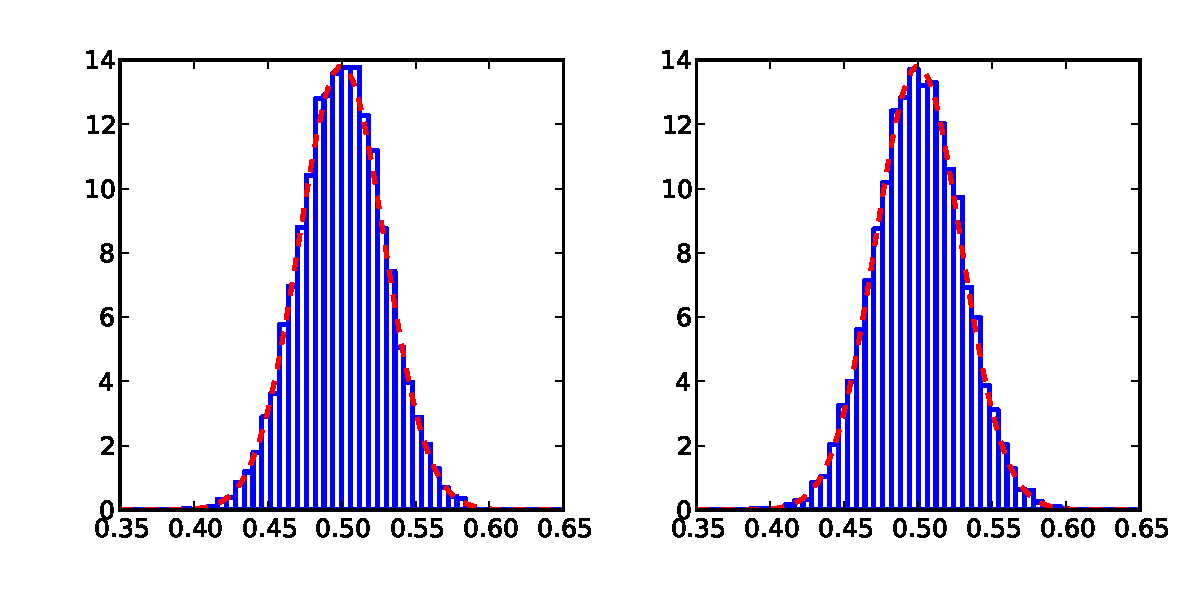
\includegraphics[width=\textwidth]{plots/statistics_test}
  \caption{Verteilung von $\overline{x} = \sum_{i=1}^{100} x_i$,
    ermittelt aus 20,000$\times$100 Werten der Zufallsgeneratoren
    \texttt{rand} (links) und \texttt{minstd} (rechts). Rot
    gestrichelt ist jeweils die erwartete Normalverteilung mit Varianz
    $\nicefrac{1}{\sqrt{1200}}$ eingezeichnet.}
  \label{fig:statistics_test}
\end{figure}

Sind die erzeugten Zufallszahlen $x_i$ tatsächlich gleichverteilt auf
$[0,1]$, so gilt für den Mittelwertschätzer
\begin{equation}
  \mean{\overline{x}} =
  \mean{\frac{1}{N} \sum_{i=1}^N x_i}
  = \mean{x} = \frac{1}{2}
\end{equation}
und für dessen Varianz nach \eqref{eq:esterr}
\begin{equation}
  \sigma(\overline{x}) = \frac{1}{\sqrt{N}} \sigma(x) =
  \frac{1}{\sqrt{12 N}}.
\end{equation}
Für immer größere $N$ sollte daher $\overline{x}$ gegen
$\nicefrac{1}{2}$ konvergieren.

Wird $\overline{x}$ sehr oft für disjunkte Zufallszahlenmengen $\{x_i,
i=1(1)N\}$ gemessen, so sollte $\overline{x}$ außerdem für große $N$
gemäß dem Gesetz der großen Zahlen praktisch normalverteilt sein, mit
der oben angegebenen Varianz. Dies kann mit Hilfe von
\eqref{eq:varest} überprüft werden, man kann aber auch direkt das
Histogram der Verteilung von $\overline{x}$ darauf überprüfen, dass es
wie erwartet normalverteilt ist.  Abbildung~\ref{fig:statistics_test}
zeigt die Verteilung von $\overline{x}$ am Beispiel von
\texttt{MINSTD} und \texttt{rand}, sowie die erwartete
Normalverteilung.  Diese Art von Test wird auch als $\chi^2$-Test
bezeichnet.

\subsubsection{Poincar\'e-Schnitte}
\index{Würfeltest}\index{Quadrattest}

\begin{figure}
  \centering
  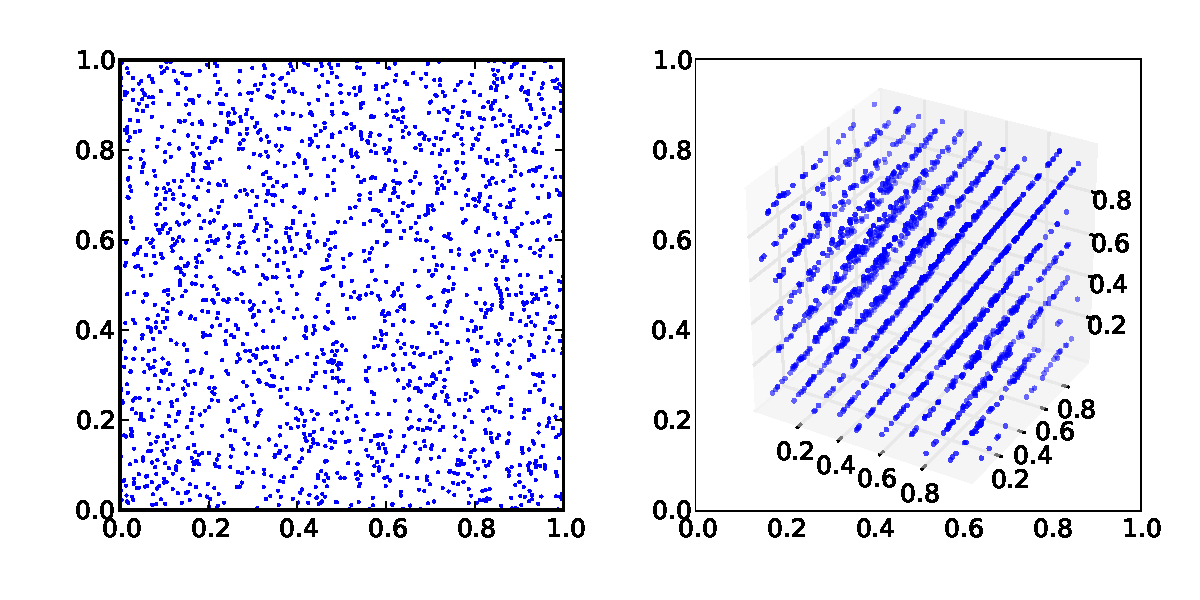
\includegraphics[width=\textwidth]{plots/optical_test}
  \caption{Quadrat- und Würfeltest mit 2,000 Auswertung am Beispiel
    des berüchtigten \texttt{RANDU}-Zufallszahlengenerators. Der
    zweidimensionale Poincar\'e-Schnitt ist homogen und unauffällig,
    aber in drei Dimensionen fallen die nur sehr wenigen Hyperebenen
    des Generators deutlich auf.}
  \label{fig:optical_test}
\end{figure}

Lineare Kongruenzgeneratoren haben nach einem Satz von Marsaglia die
Eigenschaft, dass im $\RR^n$ $n$ aufeinanderfolgende Zufallszahlen,
als Vektor aufgefasst, auf Hyperebenen liegen. Problematisch wird
dies, wenn die Anzahl der Hyperebenen sehr klein ist. Für $n=2$ und
$3$ kann man das sehr bequem überprüfen, in dem man den
Poincar\'e-Schnitt $(x_k, x_{k+1})$, $k=0,1,\ldots$ bzw. sein
dreidimensionales Äquivalent $(x_k, x_{k+1}, x_{k+2})$, $k=0,1,\ldots$
betrachtet. Da alle Punkte in $[0,1]^2$ bzw $[0,1]^3$ liegen, heißen
dieses Tests auch Quadrat- oder Würfeltests. Diese Punktwolken sollten
das Quadrat bzw. den Würfel homogen füllen und keine Strukturen
aufweisen. In zwei Dimensionen können wir das sehr rasch erfassen, in
drei Dimensionen muss man die Punktewolke rotieren, um nach
Hyperebenen zu suchen.

Abbildung~\ref{fig:optical_test} demonstriert dies für den
berüchtigten \texttt{RANDU}-LCG ($m=2^{31}$, $a=65,539$,
$b=0$). Dieser ist wegen des $2^{31}$-Moduls sehr schnell auf
32-Bit-Rechnern zu implementieren und war daher früher sogar auf
einigen Großrechnern zu finden. In der zweidimensionalen Darstellung
sind keine Auffälligkeiten zu sehen, aber ausgerechnet in den
physikalisch wichtigen drei Dimensionen zeigt sich, dass es lediglich
eine Handvoll verschiedener Hyperebenen gibt, so dass mit diesem
Generator erzeugte 3d-Vektoren kaum als zufällig gelten können.

\subsubsection{\keyword{Fouriertest}}
\index{Spektraltest}

\begin{figure}
  \centering
  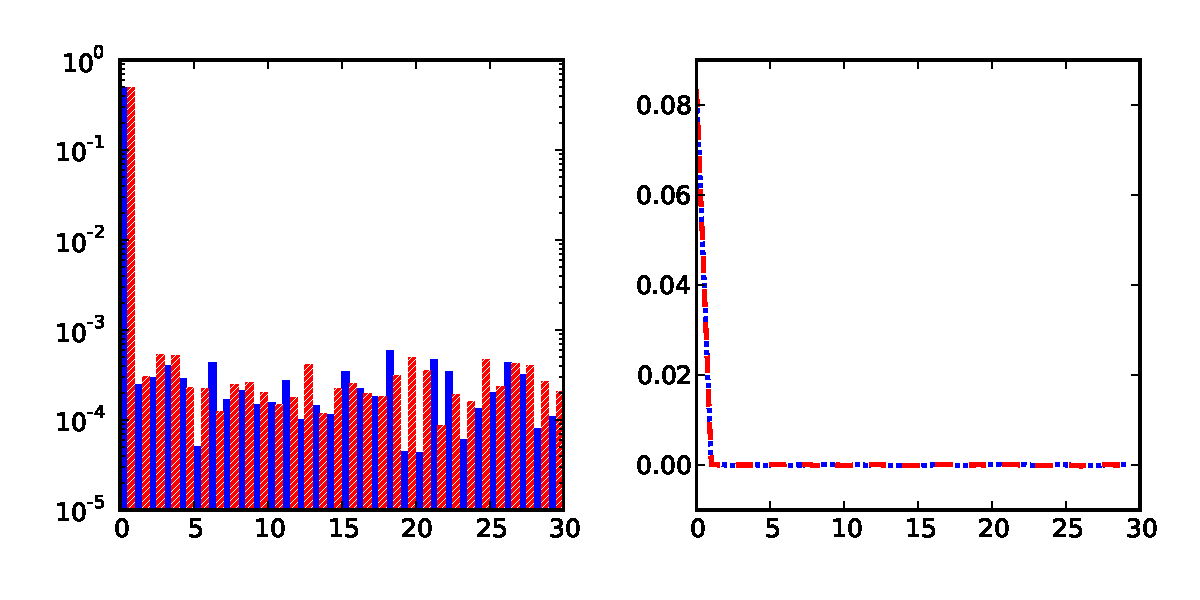
\includegraphics[width=\textwidth]{plots/fft_tests}
  \caption{Spektraltest (links) und Autokorrelationsfunktion (rechts)
    für die Zufallszahlengeneratoren \texttt{rand} und
    \texttt{MINSTD}. \texttt{rand} ist als blaue Fläche bzw. gepunktet
    eingezeichnet, \texttt{MINSTD} rot gestrichelt.  Im linken Graph
    sind die DFT-Amplituden normiert dargestellt, also dividiert durch
    die Anzahl der Zufallszahlen, so dass die 0-te Mode $1/2$ beträgt.}
  \label{fig:fft_tests}
\end{figure}

Wird eine lange Reihe von Standardzufallszahlen diskret
Fourier-transformiert, so sollte die 0-te Mode eine Amplitude von
$N/2$ aufweisen, da diese ja die Summe der Zufallszahlen angibt. Alle
anderen Moden sollten vernachlässigbar kleine, gleichmässige
Amplituden haben, entsprechend einem weißen Rauschen. Die Amplituden
aller Frequenzen ungleich $0$ sollte außerdem mit der Länge der
transformierten Zufallszahlenreihe sinken. Dieser Test wird auch als
Spektraltest bezeichnet. Abbildung~\ref{fig:fft_tests} zeigt die
DFT am Beispiel von \texttt{rand} und \texttt{MINSTD}.

\subsubsection{\keyword{Autokorrelationstest}}

Neben der diskreten Fouriertransformierten kann man auch die
Autokorrelationsfunktion der Zufallsreihe $u$ bestimmen, also
\begin{equation}
  C(u,u)(k) = \frac{1}{N}\,\text{iDFT}
  \bigl(\overline{\text{DFT}(u)(n)}\,\text{DFT}(u)(n)\bigr)(k).
\end{equation}
Für eine Zufallsreihe sind alle paarweise verschiedenen Werte
unkorreliert, also muss
\begin{equation}
  C(u,u)(k) = \sigma^2(u)\delta_k = \frac{1}{12}\delta_k
\end{equation}
gelten. Dies ist in Abbildung~\ref{fig:fft_tests} rechts
demonstriert.

\section{Beispiel: \keyword{Random walk}}

\begin{figure}
  \centering
  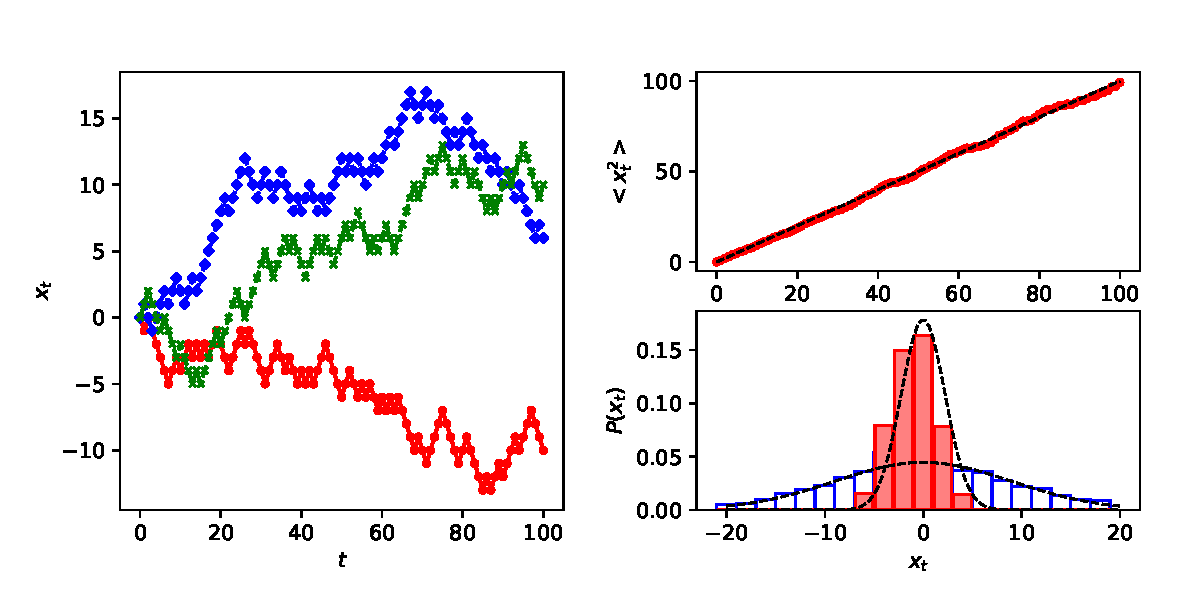
\includegraphics[width=\textwidth]{plots/rw}
  \caption{Links: 3 mögliche Random walks gemäß \eqref{eq:rw}, als
    Funktion der Zeit $t$. Rechts oben ist das mittlere
    Verschiebungsquadrat als Funktion der Zeit gezeigt, gemittelt über
    1000 Random walks. Die gestrichelte Linie markiert dabei das
    analytisch erwartete Ergebnis $\mean{x_T^2}=T$. Rechts unten
    die Verteilungen der Positionen zu den Zeitpunkten $t=5$ (rote,
    gefüllte Balken) und $t=80$ (blaue, offene Balken). Gestrichelt sind
    wieder die jeweils erwarteten Normalverteilungen eingezeichnet.}
  \label{fig:rw}
\end{figure}

Als Beispiel für die Anwendung von Zufallszahlen in der physikalischen
Simulation soll der Randomwalk ("`Irrfahrt"') dienen, der in vielen
Problemen der statistischen Physik eine Rolle spielt. Das klassische
Beispiel ist die Brownsche Bewegung von Partikeln in Wasser oder
anderen Flüssigkeiten. Diese wird durch die unzähligen Stöße der
Lösungsmittelmoleküle auf das betrachtete Teilchen erklärt.

Hat das betrachtete Teilchen einen Durchmesser von nur 1$\mu$m, so
befinden sich an seiner Oberfläche zu jedem Zeitpunkt ca. eine halbe
Milliarde Lösungsmittelmoleküle. Deren Bewegung explizit simulieren zu
wollen, ist aussichtslos. Auf der anderen Seite passieren selbst in
kurzer Zeit genügend Zusammenstöße, so dass die zeitdiskretisierte
Kraft auf das Teilchen gut als zufällig und, wegen des Gesetzes der
großen Zahlen, normalverteilt angenommen werden kann. Der Mittelwert
ist dabei offenbar Null, da die Zufallsstöße keine Vorzugsrichtung
haben sollten, die Varianz werden wir mit der Diffusionskonstanten in
Verbindung bringen.

Um diesen Prozess zu simulieren, können wir uns zunächst auf ein
eindimensionales Modell beschränken, da die Stöße in den
einzelnen Koordinaten unabhängig sind. Indem wir das Gesetz der großen Zahl
andersherum anwenden, können wir außerdem eine beliebige, aber
symmetrische Verteilung der Stöße annehmen. Die einfachste Möglichkeit
ist, einfach mit gleicher Wahrscheinlichkeit dieselbe Distanz vor-
oder zurückzugehen.

Wir betrachten also ein Teilchen mit Position $x_t$ zum Zeitpunkt
$t=1, 2,\ldots$, so dass
\begin{equation}
  \label{eq:rw}
  x_{t+1} = x_t +
  \begin{cases}
    -1 & \text{mit Wahrscheinlichkeit \nicefrac{1}{2}}\\
    +1 & \text{mit Wahrscheinlichkeit \nicefrac{1}{2}}.
  \end{cases}
\end{equation}

Ein \emph{Random walk} ist eine Folge $x_t$, die durch eine solche
einfache stochastische Bewegungsgleichung beschrieben wird.
Abbildung~\ref{fig:rw} zeigt links drei mögliche solche Random
walks. Sie wurden durch eine Routine ähnlich der folgenden generiert: 
\begin{lstlisting}
def rw(N):
    x = 0
    xt = [ x ] 
    for move in randint(0,2,N):
        if   move == 0: x += -1
        elif move == 1: x +=  1
        xt.append(x)
    return xt
\end{lstlisting}

Dieses Modell ist so einfach, dass wir seine statistischen
Eigenschaften fast vollständig analytisch berechnen können. So ist zum
Beispiel
\begin{equation}
  \mean{x_t} = \mean{\sum_{s=1}^{t} u_s} = 0, 
\end{equation}
wobei $u_{s} = x_{s} - x_{s-1}$ den $s$-ten Schritt des Random walks
bezeichnet, und daher $\mean{u_s} = 0$ gilt. Die mittlere Position des
Random walks bleibt also stets am Ausgangspunkt. Allerdings wird die
Verteilung der Punkte $x_t$ mit $t$ immer breiter, denn für das
mittlere Verschiebungsquadrat gilt
\begin{equation}
  \label{eq:sigmarw}
  \mean{x_t^2} =
  \mean{\sum_{s,r=1}^{t} u_su_r} = \sum_{s=1}^{t}\mean{u_s^2}
  = t\sigma^2(u_s) = t.
\end{equation}
Für hinreichend große $t$ kennen wir damit auch die
Wahrscheinlichkeitsdichte der Positionen, die gemäß dem Gesetz der
großen Zahlen praktisch Gaußsch ist:
\begin{equation}
  \rho(x, t) = \rho(x_t) \approx \frac{1}{\sqrt{2\pi\sigma^2}}
  \exp\left(-\frac{x_t^2}{2\sigma^2}\right).
\end{equation}
Die Varianz ist dabei $\sigma^2 = \sigma^2(x_t) = \mean{x_t^2}$, also
das mittlere Verschiebungsquadrat.

Abbildung~\ref{fig:rw} zeigt rechts oben das mittlere
Verschiebungsquadrat $\sigma^2(x_t)$, gemittelt über 1,000 Random
walks. $\sigma^2(x_t)$ ist tatsächlich mit guter Genauigkeit ungefähr
$t$, wobei die Abweichung für große $t$ größer sind, da dort die
Verteilung von $x_t$ breiter ist, und damit auch der Fehlerbalken der
Varianz. Rechs unten werden für $t=5$ und $t=80$ die Verteilungen der
Positionen gezeigt. Selbst für $t=5$ werden diese gut durch die
Gaußglocke beschreiben.  Trotzdem sollte man sich erinnern, dass die
Verteilung nicht wirklich Gaußsch ist, da offenbar $\abs{x_t}\le t$
gilt. Denn der maximale Abstand ist erreicht, wenn wir $t$-mal nur
nach links oder rechts gehen. Während also die Gaußverteilung
prinzipiell beliebig hohe Werte mit sehr kleiner Wahrscheinlichkeit
zulässt, ist die tatsächliche Verteilung beschränkt.

Das Modell lässt sich leicht auf mehrere Dimensionen erweitern, denn
die Zufallsbewegungen in den einzelnen Koordinaten sind ja
unabhängig. Die mittlere Position des Random walks in $n$ Dimensionen
ist damit immer noch konstant gleich der Ausgangsposition, das
mittlere Verschiebungsquadrat die Summe der Verschiebungsquadrate der
Koordinaten, also $\mean{x_t^2} = n t \sigma^2(u)$, wobei
$\sigma^2(u)$ das Verschiebungsquadrat der einzelnen Dimensionen
bezeichnet.

\subsubsection{Diffusion}

Was ist nun die Bedeutung von der Konstanten $D=\sigma^2(u) =
\sigma^2(x_t)/t$?  Wir verallgemeinern den Random walk, der bisher in
Zeit um $\Delta t=1$ und Raum um $\pm\Delta x = \pm 1$ gesprungen ist,
auf beliebige Werte $\Delta x$ und $\Delta t$. Dann gilt offenbar $D =
\sigma^2(u) = \Delta x^2/\Delta t$. Wir betrachten nun die
Master-Gleichung der diskreten Wahrscheinlichkeitspopulationen
\begin{equation}
  \Delta p(x, t + \Delta t) = p(x, t + \Delta t) - p(x, t) =
  \frac{1}{2}p(x - \Delta x, t) +
  \frac{1}{2}p(x + \Delta x, t) - p(x, t).
\end{equation}
Die erste Term der rechten Seite besagt, dass das Teilchen beim Sprung
$t\to t +\Delta$ mit Wahrscheinlichkeit $\frac{1}{2}$ an der Stelle
$x$ landet, wenn es sich zum Zeitpunkt $t$ an der Stelle $x-\Delta x$
befand. Der darauffolgende Term bedeutet dasselbe für $x+\Delta$, und
der letzte Term, dass das Teilchen nicht an der aktuellen Stelle
bleiben kann.

\begin{figure}
  \centering
  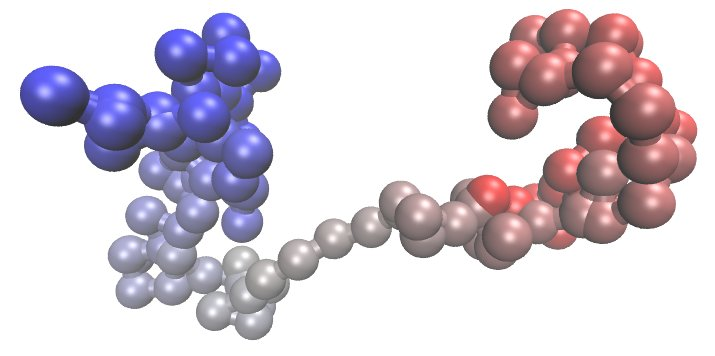
\includegraphics[width=0.6\textwidth]{plots/polymer}
  \caption{Kontinuierlicher Random walk als einfaches Polymermodell mit
    $n=100$ Monomeren. Das Polymer wurde mit der Simulationssoftware
    \textsc{ESPResSo}~\cite{espresso} erzeugt und dem
    Visualisierungstool \texttt{VMD}~\cite{vmd} gezeichnet.}
  \label{fig:contrw}
\end{figure}

Wir multiplizieren nun linker Hand mit $\Delta t^{-1}$ und rechter Hand mit
$\Delta x^{-2}$:
\begin{equation}
  \frac{\Delta p(x, t + \Delta t)}{\Delta t} =
  \frac{D}{2\Delta x^2} \left(p(x - \Delta x, t) +
    p(x + \Delta x, t) - 2 p(x, t)\right).
\end{equation}
Lassen wir nun $\Delta t\to 0$ und $\Delta x\to 0$ gehen, wird aus
dieser Gleichung die Differentialgleichung
\begin{equation}
  \frac{\delta p}{\delta t} p(x, t) =
  D\frac{\delta^2 p}{\delta x^2} p(x, t).
\end{equation}
Dies ist nichts anderes als die Diffusionsgleichung mit
Diffusionskonstante $D$. Die Varianz $D=\sigma^2(u)$ unseres
Zufallsschritts ist also genau die Diffusionskonstante unserer
makroskopischen Teilchen, und durch geeignete Wahl von $\sigma^2(u)$
können wir die Diffusionskonstante unserer Random walk-Teilchen
einstellen.

\subsubsection{Random walks als Polymermodell}
\index{Random walk>kontinuierlicher}

Man kann für den mehrdimensionalen Random walk leicht zeigen, dass es
keinen wesentlichen Unterschied macht, wenn die nächsten Positionen
nicht diskret $\pm 1$ in allen Dimensionen gewählt werden, sondern zum
Beispiel kontinuierlich oder auf einer Sphäre, d.h.,
\begin{equation}
  x_{t+1} = x_t + u \quad\text{mit}\; \norm{u}=1,\,u\text{ gleichverteilt}.
\end{equation}
Ein solcher kontinuierlicher Random walk kann mit Hilfe von
\eqref{eq:2sphere} leicht numerisch erzeugt werden, ein Beispiel ist
in Abbildung~\ref{fig:contrw} gezeigt.

Die letztere Wahl ist ein einfaches Modell für Polymere unter
bestimmten Voraussetzungen (in einem sogenannten
$\theta$-Lösungsmittel).  In diesem Fall ist $t$ allerdings keine
Zeitachse, sondern zählt einfach die Monomere entlang der Polymerkette
durch.

In guten Lösungsmitteln streckt sich das Polymer etwas mehr. Auch dies
lässt sich durch einen Random walk modellieren, bei dem die Monomere
eine endliche Ausdehnung haben und nicht überlappen können. Ein
solcher Random walk heißt auch \emph{Self avoiding walk}, weil er sich
selbst nicht kreuzen kann. In unserem einfachen Random walk-Modell
\eqref{eq:rw} entspricht das der Bedingung $x_t\neq x_s$ für alle
$s\neq t$ und ist auf dem Computer relativ einfach zu erstellen.

Um einen Self avoiding walk zu generieren, erzeugt man einfach einen
Random walk, und überprüft mit jedem neuen Punkt, ob dieser einem
anderen Monomer näher kommt als die Größe der Monomere zulässt. In
diesem Fall muss man allerdings ganz von vorne beginnen, da sonst
extrem ungünstige Konfigurationen bevorzugt werden. Bei diesen würde
ja quasi beliebig lange probiert, den nächsten Punkt zu setzen, selbst
wenn es nur eine verschwindend geringe Wahrscheinlichkeit gibt, diesen
Punkt zufällig zu treffen. Daher werden taschenartige Konfigurationen
sehr viel wahrscheinlicher, als sie zufällig auftreten würden. Ab etwa
100 Monomeren ist die Wahrscheinlichkeit, einen Random walk
abzulehnen, schon sehr hoch, und die Erzeugung eines Self avoiding
walks dementsprechend aufwändig.

Auch von der Theorie her ist der Self avoiding walk sehr viel
komplizierter. So gilt etwa $\mean{x_N^2} \sim N^{2\nu}$ mit
$\nu\approx 0.588$, so dass das Polymer im Mittel tatsächlich etwas
mehr gestreckt ist als der Random walk mit $\nu=\nicefrac{1}{2}$. Der
Wert von $\nu$ für den Self avoiding walk kann, anders als beim Random
walk, nicht analytisch berechnet werden, sondern nur aufwändig
numerisch genähert.

Der Self avoiding walk wie auch der der einfache Random walk spielen
nach wie vor eine wichtige Rolle in der Polymerphysik, insbesondere
beim Aufsetzen von Polymersimulationen. Daher besitzt etwa
Simulationssoftware \textsc{ESPResSo}~\cite{espresso} einen eigenen
Befehl, um solche Zufallsketten zu erzeugen.

\subsubsection{Diffusionslimitierte Aggregation}

\begin{figure}
  \centering
  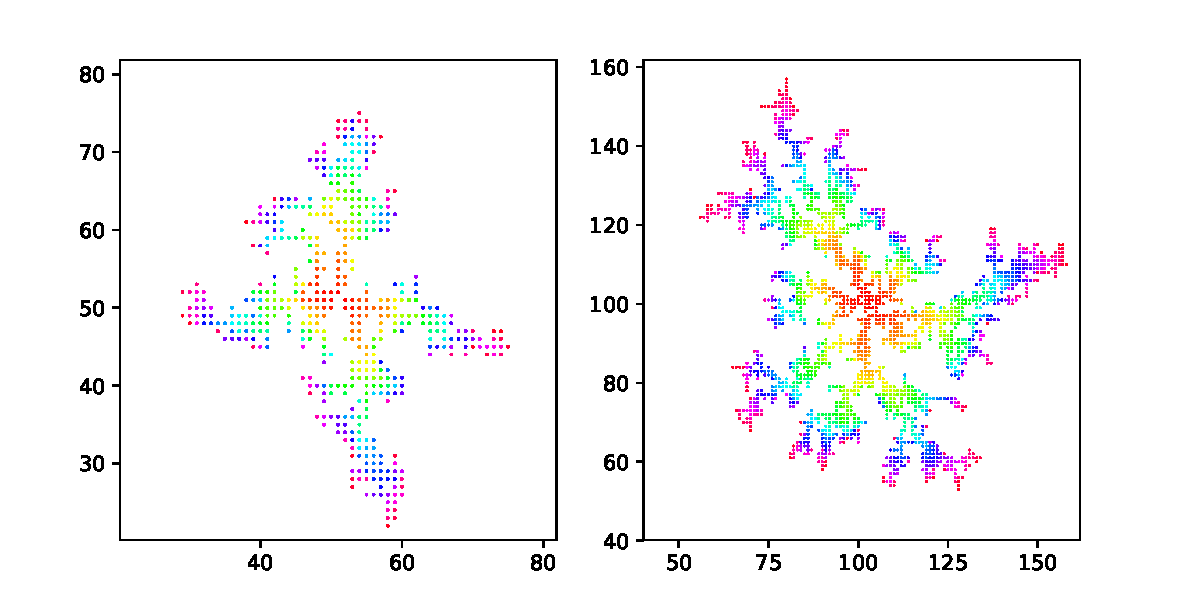
\includegraphics[width=\textwidth]{plots/dla}
  \caption{Cluster aus diffusionslimitierter Aggregation mit $N=500$
    (links) und $N=2000$ (rechts) Teilchen. Die Teilchen sind in der
    Reihenfolge der Anlagerung farblich codiert.}
  \label{fig:dla}
\end{figure}

Eine weitere Anwendung des Random walks ist die diffusionslimitierte
Aggregation, die etwa die Bildung von Rußaggregaten modelliert. Dabei
wird davon ausgegangen, dass sich diese aus einem Keim durch
Anlagerung von weiteren Teilchen bilden, die aus dem Unendlichen heran
diffundieren.

Für die Modellierung werden Random walks genutzt, die zufällig auf
einer Kugelsphäre um den Keim gestartet werden, bis sie entweder am
Cluster anlagern oder sich zu weit vom Kreis entfernt
haben. Abbildung~\ref{fig:dla} zeigt zwei solche DLA-Cluster mit 500
und 2000 Teilchen auf einem zweidimensionalen Gitter. Die beiden
Cluster haben eine sehr ähnliche Struktur, auch wenn die Maßstäbe
deutlich anders sind. Das hängt damit zusammen, dass solche
diffusionslimitierte Aggregate selbstähnliche Fraktale
sind. Listing~\ref{lst:dla} zeigt den Python-Code zur Erzeugung
solcher zweidimensionaler DLAs.

Die zentrale Frage beim Studium von DLA-Clustern ist die nach ihrer
fraktalen Dimension. In drei Dimensionen legen wir zu ihrer Bestimmung
konzentrische Kugeln mit Radius $R$ um den Keim eines sehr großen
Clusters, und zählen die Anzahl der Teilchen $N(R)$ in dieser
Kugel. Die fraktale Dimension ist dann
\begin{equation}
  d = \lim_{R\to\infty}\frac{\log N(R)}{\log R}.
\end{equation}
In der Praxis betrachtet man natürlich einfach mehrere große Cluster
verschiedener Größe, um $d$ abzuschätzen.  Wäre der Cluster solide mit
Teilchendichte $\rho$, so wäre $N(R) = \rho \frac{4\pi}{3} R^3$ und
\begin{equation}
  \frac{\log N(R)}{\log R} = \frac{\log\left( \rho
      \frac{4\pi}{3} R^3\right)}{\log R} =
  3 + \frac{\log\left( \rho\frac{4\pi}{3}\right)}{\log R},
\end{equation}
die fraktale Dimension also wie erwartet 3. Der DLA-Cluster in drei
Dimensionen hat übrigens eine fraktale Dimension von $\approx 1,6$,
ist also bei weitem kein solides Objekt. Daher werden solche Cluster
gerne als Katalysatoren verwendet, da sie eine entsprechend große
Oberfläche haben.

\raggedbottom \lstinputlisting[style=multipage, caption={Code zur
  Erzeugung eines DLA-Clusters auf einem zweidimensionalen Gitter
  \argd{world}. Die Eingabeparameter sind die Größe \argd{M} des
  Gitters, sowie die Anzahl der Punkte des zu erzeugenden Aggregats
  \argd{N}. Das Aggregat entsteht durch sukzessive Anlagerung mit
  Hilfe von Random walks, die auf einem langsam wachsenden Kreis um
  das aktuelle Aggregat starten. Der Radius \argd{R} diese Kreises ist
  stets um 5 Gittereinheiten größer als der Umkreis des Clusters.},
label=lst:dla]{dla.py}

\section{Beispiel: \keyword{Perkolation}}

Ein anderes Beispiel eines Zufallsalgorithmus ist die Perkolation,
also die Frage, wann ein Zufallsmedium einen durchgehenden Kanal
zulässt oder nicht. Anwendungsbeispiele sind etwa poröse Medien, die
Flüssigkeiten nur passieren lassen, falls es einen durchgehenden
Hohlraum gibt, oder eine Mischung von Isolator und Leiter, die nur
leitet, wenn es eine leitende Verbindung gibt.

Modellieren lässt sich dies als ein Gitter, dessen Zellen mit einer
gewissen Wahrscheinlichkeit $p$ besetzt sind. Die Frage ist dann, ab
welcher kritischen Wahrscheinlichkeit $p_c$ es im Regelfall einen
Cluster von benachbarten, besetzten Feldern gibt, der das gesamte
System in einer Richtung durchzieht, man sagt,
\emph{perkoliert}. Diese Grenze lässt sich durch Untersuchen sehr
vieler zufälliger Besetzungen untersuchen.

Die Besetzungen sind dabei natürlich durch stochastisches Belegen des
Gitters sehr einfach zu erzeugen, algorithmisch etwas schwieriger ist
nur, zu bestimmen, ob es einen perkolierenden Cluster gibt, also
einen, der eine Seite mit der gegenüberliegenden verbindet.

Eine Möglichkeit ist, die Struktur von einer Seite aus gewissermaßen
zu "`fluten"', und zu sehen, ob man dabei die gegenüberliegende Seite
erreicht. Erreichen heißt hier, dass es einen zusammenhängenden Pfad
von paarweise benachbarten, besetzten Punkten gibt. Um dies zu
überprüfen, erzeugen wir zunächst eine Liste der besetzten Punkte am
Start\-rand.  Dann fügen wir zu dieser Liste alle benachbarten Punkte
hinzu, und wiederholen dies solange, bis keine neuen Elemente mehr zur
Liste hinzugefügt wurden. Die Liste enthält dann alle Punkte, die
Verbindung zum Startrand haben. Wir müssen nur noch überprüfen, ob in
dieser Liste Punkte am gegenüberliegenden Rand auftauchen.

\begin{figure}
  \centering
  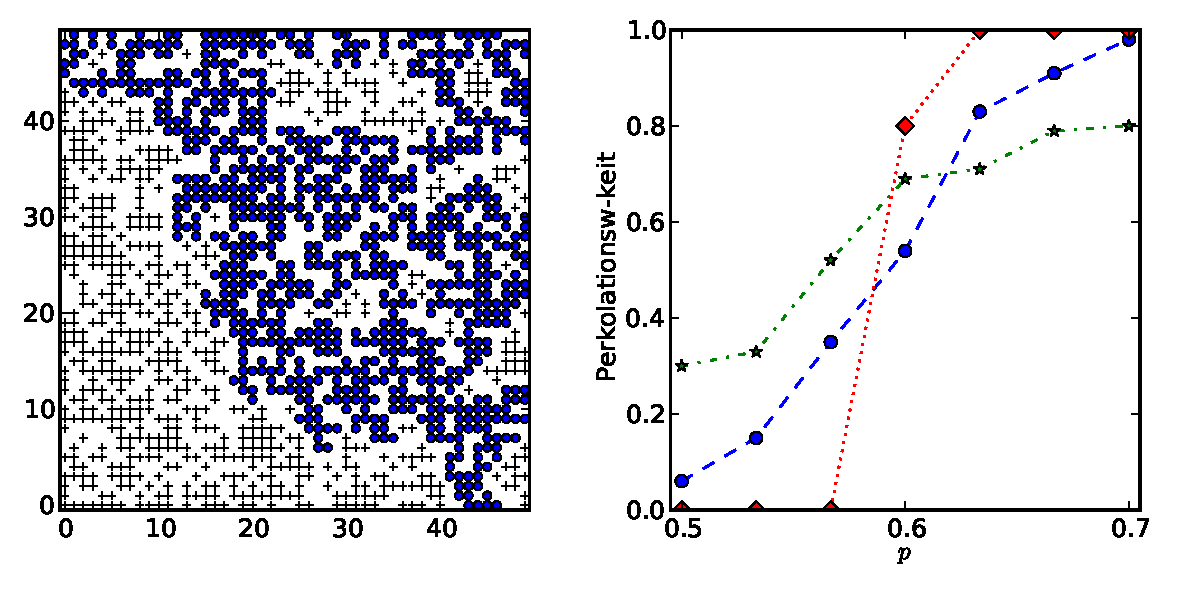
\includegraphics[width=\textwidth]{plots/percolation}
  \caption{Ein perkolierender Cluster auf einem $50^2$-Gitter mit
    $p=0,6$. Blaue Punkte markieren den Cluster, Kreuze andere, mit
    diesem Cluster nicht verbundene, aber besetzte Gitterpunkte. Im
    rechten Graph ist für $L=5$ (grüne Sterne), $L=20$ (blaue
    Diamanten) und $L=100$ mit welcher Wahrscheinlichkeit bei
    Besetzung $p$ ein perkolierender Cluster gefunden wurde. Für
    $L=100$ ist dies ein bereits sehr scharfer 0--1-Übergang in Nähe
    von $0,6$.}
  \label{fig:percolation}
\end{figure}

In dieser Form wäre der Algorithmus recht langsam, weil man ständig
wieder Punkte hinzufügen würde, die bereits in der Liste sind, und
diese erneut untersucht. Um dies zu vermeiden, führt man einfach eine
zweite Liste der Punkte, deren Nachbarn noch nicht untersucht
wurden. Ein Punkt, der noch nicht in der Liste der verbunden Punkte
steht, wird dann nicht nur zu dieser, sondern auch zur Liste der zu
bearbeitenden Punkte hinzugefügt. Dann müssen nur die Nachbarn der
Punkte in dieser Liste betrachtet werden, und sobald die Nachbarn
eines Punkts einmal untersucht wurden, kann dieser aus der Liste der
zu bearbeitenden Punkte gestrichen werden. Da er aber immer noch als
verbunden markiert ist, wird er auch nie ein zweites Mal in die Liste
der zu bearbeitenden Punkte eingefügt werden. Der Algorithmus
terminiert also, da die abzuarbeitende Liste irgendwann leer ist. Ein
entsprechendes Python-Skript ist in Listing~\ref{lst:percolation} zu
sehen.

Abbildung~\ref{fig:percolation} zeigt links einen perkolierenden
Cluster für ein Gitter mit Besetzungwahrscheinlichkeit $p=0,6$, es
sind also etwas mehr als die Hälfte der Punkte besetzt. Rechts ist für
verschiedene Besetzungswahrscheinlichkeiten aufgetragen, wie
wahrscheinlich es ist, einen perkolierenden Cluster zu beobachten. Wie
man sieht, ist $p=0,6$ nicht ohne Grund gewählt, denn dies ist sehr
dicht am kritischen Perkolationsschwellwert. Der tatsächliche Wert des
Schwellwerts ist $p_c\approx 0,593$ im Limit unendlicher Gittergröße,
wie man zeigen kann. Mit steigender Kantenlänge wird der Übergang
bereits bei endlichen Gittern relativ scharf, bei $L=100$ ist der
Grenzbereich weniger als $0,06$ in $p$ breit. Bei einer Besetzung von
$0,56$ ist Perkolation äußerst unwahrscheinlich, bei $0,6$ gibt es
hingegen schon für die Mehrheit der Gitter einen perkolierenden
Cluster.

Ähnlich wie beim Random walk kann auch die Perkolation in unzähligen
Variationen betrachtet werden, etwa andere zugrundeliegende Gitter,
höhere Dimensionen oder auch kontinuierliche Modelle.

\raggedbottom \lstinputlisting[style=multipage,
caption={Code zur Schätzung des Perkolationsschwellwerts auf einem
  zweidimensionalen quadratischen Gitter \argd{world}. Die Liste
  \argd{connected} enthält die alle Punkte, die mit dem oberen Rand
  verbunden sind, die Liste \argd{connected_undone} diejenigen
  verbundenen Punkte, deren Nachbarn noch untersucht werden
  müssen.}, label=lst:percolation]{percolation.py}

%%% Local Variables: 
%%% mode: latex
%%% TeX-master: "padc"
%%% TeX-PDF-mode: t
%%% End: 

% Dies ist Teil der Vorlesung Physik auf dem Computer, SS 2012,
% Axel Arnold, Universitaet Stuttgart.
% 
% Dieses Werk ist unter einer Creative Commons-Lizenz vom Typ
% Namensnennung-Weitergabe unter gleichen Bedingungen 3.0 Deutschland
% zugänglich. Um eine Kopie dieser Lizenz einzusehen, konsultieren Sie
% http://creativecommons.org/licenses/by-sa/3.0/de/ oder wenden Sie sich
% schriftlich an Creative Commons, 444 Castro Street, Suite 900, Mountain
% View, California, 94041, USA.

\chapter{Lineare Algebra \textrm{II}}
\index{Gleichungssysteme>lineare}

Wie wir bereits an der Besselgleichung gesehen haben, lassen sich
gewöhnliche Differentialgleichungen in einer Dimension recht einfach
auf lineare Gleichungssysteme abbilden. Diese haben Bandstruktur und
sind effizient zu lösen.  In mehr als einer Dimension ist das
allerdings im allgemeinen nicht mehr der Fall. Betrachten wir zum
Beispiel die Poissongleichung in zwei Dimensionen:
\begin{equation}
  \label{eq:laplace}
  \Delta \phi = \frac{\partial^2 \phi}{\partial x^2} +
  \frac{\partial^2 \phi}{\partial y^2} = \rho.
\end{equation}
Wir diskretisieren nun wie gewohnt $\phi(x,y)$ in beiden Dimensionen
zu $\phi_{k, l} = \phi(k h, l h)$, $k,l=(1)N$. Den Laplace-Operator
erhalten wir dann in erster Ordnung als
\begin{align}
  \label{eq:laplacedisc}
  \Delta \phi(k h, l h) \approx
  \frac{1}{h^2}\bigl(\phi_{k+1,l} -
  2\phi_{k,l}  + \phi_{k-1,l}\bigr) + 
  \frac{1}{h^2}\bigl(\phi_{k,l+1} -
  2\phi_{k,l}  + \phi_{k,l-1}\bigr)\nonumber\\
  = \frac{1}{h^2}\bigl(
  \phi_{k,l+1} + \phi_{k+1,l} - 4\phi_{k,l} +
  \phi_{k-1,l} + \phi_{k,l-1}\bigr).
\end{align}
Der Einfachheit halber nehmen wir periodische Randbedingungen an, so
dass wir diese Gleichung für jeden Gitterpunkt aufstellen
können. Allerdings wäre die resultierende Matrix singulär; um die
Differenzialgleichung mit periodischen Randbedingungen eindeutig lösen
zu können, müssen wir einen Funktionswert vorgeben.

Diese Gleichungen sind im Moment noch auf der Matrix $\phi_{k,l}$
definiert, die wir nun \emph{linearisieren} müssen, um die Gleichung
in der gewohnten Matrixform etwa an Python zu übergeben. Hierzu
speichern wir die Elemente von $\phi_{k,l}$ wie folgt:
\begin{equation}
  \Phi_{k + N l} = \phi_{k,l} \quad\text{für}\; k,l=1(1)N.
\end{equation}
Wie man sich leicht überlegt, ist diese Zuordnung eindeutig, wir
können also beliebig zwischen $\Phi_n$ und $\phi_{k,l}$ wechseln und
so etwa \eqref{eq:laplacedisc} auf den Vektor $\Phi_n$
übertragen. Dies ergibt dann $N^2$ Gleichungen für alle Datenpunkte,
die in Matrixform für $N=5$ zum Beispiel wie folgt aussehen:
\begin{equation}
  \label{eq:2d-laplace}
  \left( \text{\raisebox{-4\baselineskip}{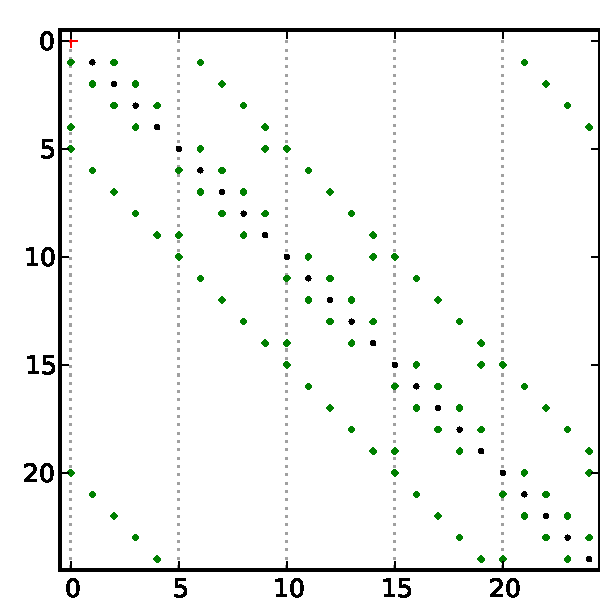
\includegraphics[height=8.5\baselineskip]{plots/2d-laplace}}} \;\right)
  \;\cdot\begin{pmatrix}
    \Phi_0 = \phi(0,0)\\
    \Phi_1 = \phi(h,0)\\
    \vdots\\
    \Phi_{4} = \phi(h,0)\\
    \Phi_{5} = \phi(0,h)\\
    \vdots\\
    \Phi_{24} = \phi(4h,4h)
  \end{pmatrix}
  =
  \begin{pmatrix}
    \Phi_0\\
    \rho(h,0)\\
    \vdots\\
    \rho(h,0)\\
    \rho(0,h)\\
    \vdots\\
    \rho(4h,4h)
  \end{pmatrix}
  .
\end{equation}
In der Matrix markieren grüne Punkte Einträge mit Wert $1/h^2$,
schwarze Punkte Einträge mit Wert $-4/h^2$ und das rote Kreuz den
Normierungseintrag mit Wert 1. Alle anderen Einträge sind Null.

Durch die periodischen Randbedingungen in $x$ und $y$ sind zwei
Nebendiagonalen weiter außen teilweise besetzt. Damit hat die
entstehende Matrix zwar immer noch Bandstruktur hat und ist dünn
besetzt, d.h. fast alle Einträge Null, allerdings ist sie nicht mehr
tridiagonal. Auch durch Umsortieren lässt sich dies nicht wesentlich
ändern, daher muss die volle Gaußelimination durchgeführt werden. Für
Gitter von $5\times 5$ Punkten ist das zwar noch unproblematisch, bei
einem Gitter von $100\times 100$ Punkten hat die volle Matrix
allerdings bereits $100,000,000$ Einträge, und die Gaußelimination
wird zu langsam. Noch schwieriger wird es in den meist benutzten
drei Dimensionen, da die volle Matrix schnell mehrere Milliarden
Einträge hat.

Neben der Ineffizienz des Gaußverfahrens bringt das Arbeiten mit der
vollen Matrix allerdings auch Speicherprobleme mit sich, denn eine
volle Matrix aus dem $\RR^{100,000\times 100,000}$ benötigt bei
einfacher Genauigkeit über 37GB Speicher. Dünn besetzte Matrizen
dieser Größe sind allerdings durchaus handhabbar, denn nur wenige
Matrixelemente sind überhaupt ungleich Null. Indem man nur diese
Elemente geschickt speichert, lassen sich sogar noch weitaus größere
Matrizen bewältigen. Auf derartigen Datenstrukturen kann die
Gaußelimination allerdings nicht effizient eingesetzt werden, da diese
die Matrixstruktur durch die Zeilenadditionen rasch zerstört.

Im folgenden lernen wir nun schnellere, iterative Gleichungslöser
kennen, mit denen auch solche und größere Gleichungssysteme handhabbar
werden. Außerdem können diese Verfahren auch auf große, dünn besetzte
Matrizen angewandt werden. Weiter lernen wir die QR-Zerlegung als
weitere Matrixzerlegung kennen, die eine wichtige Rolle bei der
Bestimmung von orthogonalen Basen und der 
Optimierung spielt. Sie kann auch zur Berechnung von Eigenwerten und
-vektoren benutzt werden, was dieses Kapitel abschließt.

\section{Iterative Gleichungslöser}

Wir betrachten eine reguläre Matrix $A\in\RR^{n,n}$ und einen Vektor
$b\in\RR^n$. Gesucht ist dann die Lösung $\overline{x}\in\RR^n$ mit
\begin{equation}
  \label{eq:axb}
  A\overline{x} = b.
\end{equation}

Die Gaußelimination liefert diese bei unendlicher Genauigkeit exakt,
allerdings mit dem hohen Aufwand $\O(n^3)$. Wir haben allerdings
bereits gesehen, dass iterative Verfahren wie etwa das Newtonverfahren
zur Lösung nichtlinearer Gleichungssysteme quadratisch
konvergieren. Hierzu gibt es mehrere mögliche Ansätze, etwa das
CG-Verfahren, das auf einem Optimierungsproblem beruht und das wir
später kennenlernen werden. Zunächst suchen wir aber iterative
Verfahren der Form
\begin{equation}
  \label{eq:itgl}
  x^{(i+1)} = G(x^{(i)}) = T x_i + r
\end{equation}
mit $r\in\RR^n$ und $T\in\RR^{n,n}$, $\norm{T}<1$. Der Banachsche
Fixpunktsatz gewährleistet, dass diese sukzessive Substitution für
jeden Startwert konvergiert, wobei die Norm $\norm{\cdot}$ wiederum
geeignet gewählt werden kann.

Wie müssen wir nun $T$ wählen, damit einerseits $x^{(i)}\to \overline{x}$
für $i\to\infty$, andererseits aber $T$ und $r$ einfach zu berechnen
sind? Da $\norm{T} < 1$ sein soll, muss $r$ bereits eine
Näherungslösung sein. Es sollte also $r = B^{-1}b$ sein, wobei $B$
eine geeignete, einfach zu invertierende Näherung von $A$ ist. Dann
gilt
\begin{equation}
  \overline{x} = T\,\overline{x} +
  B^{-1}b
  \stackrel{!}{=} T\,\overline{x} +
  B^{-1}A\,\overline{x}
  = \left(T + B^{-1}A\right)\overline{x},
\end{equation}
was sich offenbar durch Wahl von $T = I - B^{-1}A$ erfüllen
lässt. Solange also $B^{-1}$ einfach zu bestimmen ist, lassen sich
sowohl $T$ als auch $r$ einfach berechnen.

\subsection{\keyword{Jacobiverfahren}}

Das erste Verfahren nach diesem Schema, dass wir kennenlernen, ist
das Jacobiverfahren. Die Matrix $A$ wird dazu als Summe einer
Diagonalmatrix sowie einer linken, unteren und einer rechten oberen
Dreiecksmatrix mit verschwindender Diagonale zerlegt, also $A = L + D
+ U$ mit
\begin{equation}
  l_{ik}=
  \begin{cases}
    a_{ik} & \text{für}\; i<k\\
    0 & \text{sonst}
  \end{cases},\quad
  d_{ik} =
  \begin{cases}
    a_{ik} & \text{für}\; i=k\\
    0 & \text{sonst}
  \end{cases}\quad\text{und}\;
  u_{ik} =
  \begin{cases}
    a_{ik} & \text{für}\; i>k\\
    0 & \text{sonst}
  \end{cases}.
\end{equation}
Die Diagonalmatrix $D$ soll dabei die Rolle der leicht zu
invertierenden Matrix übernehmen. Dazu müssen die Diagonalelemente
alle von Null verschieden sein, was sich bei einer regulären Matrix
$A$ durch Vertauschen von Zeilen und/oder Spalten immer erreichen
lässt.

Setzen wir also $T=I-D^{-1}A$ und $r=D^{-1}b$ in \eqref{eq:itgl} ein,
so erhalten wir das \emph{Jacobiverfahren}
\begin{align}
  x^{(i+1)} = \left(I - D^{-1}A\right)x^{(i)} + D^{-1}b\nonumber\\
  = -D^{-1}\left(L + U\right)x^{(i)} + D^{-1}b
\end{align}
mit der Diagonalmatrix $D$, so dass $d^{-1}_{jj} =
\frac{1}{a_{jj}}$. Komponentenweise bedeutet dies, dass
\begin{equation}
  \label{eq:jacobicomp}
  x_j^{(i+1)} = \frac{1}{a_{jj}}\left(b_j - \sum_{k\neq j} a_{jk}x_k^{(i)}\right).
\end{equation}
Mit anderen Worten, dass Jacobiverfahren löst jede Zeile nach der
Variablen auf der Diagonale auf.

\index{strikt diagonaldominant}
Wann konvergiert dieses Verfahren? Eine gängige Voraussetzung ist,
dass die Matrix $A$ strikt diagonaldominant ist, also
\begin{equation}
  \sum_{k\neq i} \abs{a_{ik}} < \abs{a_{ii}}\quad\text{für}\; i=1(1)n.
\end{equation}
Diese Bedingung ist sehr stark, zum Beispiel erfüllen weder die Matrix
aus dem Eingangsbeispiel noch etwa die für die Spline-Interpolation
benötigten Matrizen diese Bedingung, da in beiden Fällen das
Diagonalelement betragsmäßig die Summe der Nebenelemente
ist. Allerdings sind die bei der sogenannten Finite-Elemente
Modellierung zur Diskretisierung von Differentialgleichungen
entstehenden Matrizen meist strikt diagonaldominant. Daher spielen
Löser für diese Art von Matrizen auch kommerziell eine wichtige Rolle.

Ist $A$ strikt diagonaldominant, so nutzen wir die Maximumsnorm
\begin{equation}
  \norm{A}_\infty := \max_{i=1}^n \sum_{k=1}^n \abs{a_{ik}},
\end{equation}
die eine Matrixnorm definiert. Dann gilt
\begin{equation}
  \norm{T}_{\infty} = \norm{I-D^{-1}A}_{\infty} =
  \max_{i=1}^n \sum_{k\neq i} \frac{\abs{a_{ik}}}{\abs{a_{ii}}} < 1,
\end{equation}
die sukzessive Substitution und damit das Jacobiverfahren konvergieren
also. Außerdem ist die Konvergenz linear, genauer gilt
\begin{equation}
  \frac{\norm{x_{n+1} - \overline{x}}_\infty}{\norm{x_{n} - \overline{x}}_\infty}
  \le \sum_{k\neq i} \frac{\abs{a_{ik}}}{\abs{a_{ii}}},
\end{equation}
wobei $\norm{x}_\infty := \max_{i=1}^n \abs{x_i}$ die
Vektormaximumsnorm bezeichnet. Je größer also die Diagonaleinträge
gegenüber den Nebeneinträgen sind, desto schneller konvergiert das
Verfahren, zum Beispiel wenn die Matrix eine kleine Störung der
Einheitsmatrix ist.

\subsubsection{Indizierte Matrixspeicherung}
\index{indizierte Matrixspeicherung}
\index{Indexformat}

Wie man an der komponentenweisen Darstellung \eqref{eq:jacobicomp} gut
sieht, kann das Jacobiverfahren auch auf dünnbesetzten Matrizen
implementiert werden. Zum einen wird die Matrix $A$ beim Verfahren
nicht verändert, sondern nur der erheblich kleinere Lösungsvektor, zum
anderen wird nur zeilenweise summiert, was eine indizierte Speicherung
ermöglicht.  Dazu wird für jede Zeile $j$ lediglich der
Diagonaleintrag $a_{jj}$ explizit gespeichert, sowie eine Liste mit
Einträgen $(k, a_{jk})$, die die restlichen Elemente $\neq 0$
enthält. Eine Implementation des Jacobiverfahrens muss dann lediglich
für jede Zeile die Summe $\sum_{k\neq j} a_{jk}x_k^{(i)}$ mit
Hilfe der zur Zeile gehörigen Liste bilden, von $b_j$ abziehen und
durch $a_{jj}$ teilen.

In unserem einführenden Beispiel wären pro Zeile neben der Diagonalen
maximal vier weitere Einträge nötig, unabhängig davon, wie fein die
Schrittweite gewählt wird. Die Matrix \eqref{eq:2d-laplace} würde
damit so dargestellt:
{\small
  \begin{align}
    1, \{\} \;&\mathop{\widehat{=}}\; \left(1, 0, \ldots, 0\right)
    \nonumber\\
    -\frac{4}{h^2}, \left\{
      \left(3, \frac{1}{h^2}\right), \left(1, \frac{1}{h^2}\right),
      \left(7, \frac{1}{h^2}\right), \left(22, \frac{1}{h^2}\right)
    \right\}
    \;&\mathop{\widehat{=}}\;
    \left(\frac{1}{h^2}, -\frac{4}{h^2}, \frac{1}{h^2}, 0, 0, 0, 1, 0,
      \ldots, 0, 1, 0, 0, 0\right)\nonumber\\
    -\frac{4}{h^2}, \left\{
      \left(4, \frac{1}{h^2}\right), \left(2, \frac{1}{h^2}\right),
      \left(8, \frac{1}{h^2}\right), \left(23, \frac{1}{h^2}\right)
    \right\}
    \;&\mathop{\widehat{=}}\;
    \left(0, \frac{1}{h^2}, -\frac{4}{h^2}, \frac{1}{h^2}, 0, 0, 0, 1, 0,
      \ldots, 0, 1, 0, 0\right)\nonumber\\
    &\vdots\\
    a_{jj}, \left\{(k_1, a_{jk_1}),(k_2, a_{jk_2}), \ldots\right\}
    \;&
  \end{align}}

\subsection{\keyword{Gauß-Seidel-Verfahren}}

Wird \eqref{eq:jacobicomp} zeilenweise abgearbeitet, so müssen die
bereits berechneten Werte $x_j^{(i+1)}$ zwischengespeichert werden,
da für die restlichen Zeilen ja noch die alten Werte $x_k^{(i)}$
benötigt werden. Beim Gauß-Seidel-Verfahren werden stattdessen die
bereits berechneten, neueren Werte benutzt:
\begin{equation}
  \label{eq:gscomp}
  x_j^{(i+1)} = \frac{1}{a_{jj}}\left(b_j -
    \sum_{k=1}^{j-1} a_{jk}x_k^{(i+1)} - \sum_{k=j+1}^n a_{jk}x_k^{(i)}\right).
\end{equation}
Dies erspart einerseits die getrennte Speicherung der neuen
Näherungslösung $x_k$, andererseits ist die neue Näherungslösung näher
an der Lösung, so dass es durchaus sinnvoll erscheint, diese neuen, besseren
Werte für die verbleibenden Zeilen zu nutzen.

Mit der Zerlegung $A=L + D + U$ wie beim Jacobiverfahren ergibt sich
in Matrixschreibweise
\begin{equation}
  x^{(i+1)} = -D^{-1}L x^{(i+1)} - D^{-1} U x^{(i)} + D^{-1}b
  \;\implies\;
  (D + L)x^{(i+1)} = - U x^{(i)} + b
\end{equation}
und damit
\begin{equation}
  x^{(i+1)} = -(D+L)^{-1} U x^{(i)} - (D+L)^{-1}b.
\end{equation}
Das Gauß-Seidel-Verfahren ist also auch vom Typ \eqref{eq:itgl}, mit
der etwas komplexeren Matrix $B= D + L$. Tatsächlich ist auch
\begin{equation}
  \label{eq:gst}
  T = I - (D + L)^{-1} A = (D + L)^{-1}(D + L - A) = -(D+L)^{-1} U.
\end{equation}
Man kann zeigen, dass $\norm{T}_\infty$ beim Gauß-Seidel-Verfahren
kleiner ist als beim Jacobi-Verfahren. Das bedeutet allerdings im
allgemeinen nicht, dass das Gauß-Seidel-Verfahren schneller ist, trotz
dessen, dass teilweise mit prinzipiell besseren Näherungen gerechnet
wird. Man spart allerdings den Speicherplatz, um $x^{(i+1)}$
zwischenzuspeichern.

Genauso wie das Jacobiverfahren kann auch das Gauß-Seidel-Verfahren
auf indizierten Matrixformaten benutzt werden, wobei die beiden Summen
in \eqref{eq:gscomp} entweder gleichzeitig aufaddiert werden, oder die
Listen der Nichtdiagonalelemente in Elemente links und rechts der
Diagonalen aufgeteilt.

Insbesondere für die parallele Verarbeitung, die mit der heutigen
weiten Verbreitung von Mehrkern-Prozessoren ein wichtiger Faktor ist,
ist das Gauß-Seidel-Verfahren allerdings ungeeignet, da die Berechnung
jeder Zeile die Ergebnisse der vorherigen erfordert. Das
Jacobi-Verfahren kann hingegen auf so viele Prozessoren verteilt
werden, wie die Matrix Zeilen hat, was eine effiziente Verarbeitung
selbst auf modernen Graphikkarten ermöglicht.

\subsection{\keyword{Relaxationsverfahren}}
\index{Successive over-relaxation}
\index{SOR}

Beim Relaxationsverfahren (Successive over-relaxation, SOR) wird statt
$B = D + L$ die Matrix $B = D/\omega + L$ mit einem Relaxationsfaktor
$\omega$ betrachtet. Durch geeignete Wahl von $\omega$ können dann
auch nicht strikt diagonaldominante Matrizen behandelt
werden. Allerdings kann man nur zeigen, dass $0<\omega< 2$ gelten
muss, aber ein Wert $\omega$, der zu schneller Konvergenz führt, muss
durch Ausprobieren gefunden werden.

\begin{figure}
  \centering
  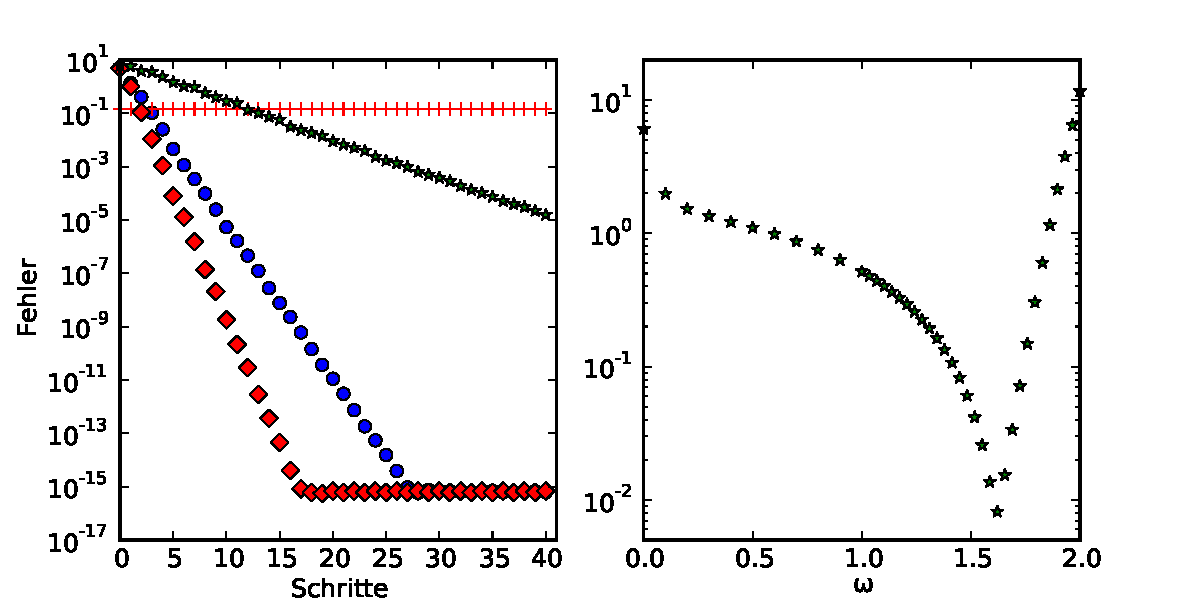
\includegraphics[width=\textwidth]{plots/iterative}
  \caption{Konvergenz von Jacobi-, Gauß-Seidel- und
    Relaxationsverfahren. Zum einen wird die Matrix $A$ aus
    \eqref{eq:2d-laplace} betrachtet, die wie gesagt nicht strikt
    diagonaldominant ist. Zum anderen wird eine Matrix $B$ mit
    genausovielen, normalverteilten Einträgen, betrachtet, die strikt
    diagonaldominant gemacht wurde, in dem $b_{i,i} = 1+ \sum_{k\neq
      i}\abs{b_{ik}}$ gesetzt wurde. Links sind die Fehler
    $\norm{Bx-b}_2$ von Jacobi- und Gauß-Seidel-Verfahren für die
    Matrix $B$ mit blauen Punkten bzw. roten Rauten eingezeichnet. Die
    roten Kreuze zeigen hingegen den Fehler des Gauß-Seidel-Verfahrens
    für die Matrix $A$, das nicht konvergiert. Grüne Sterne
    schließlich zeigen den Fehler des SOR-Verfahrens, das mit
    $\omega=1,63$ auch bei Matrix $A$ konvergiert. Der rechte Graph
    zeigt den Fehler des SOR-Verfahrens in Abhängigkeit von $\omega$
    nach 20 Schritten.}
  \label{fig:sor}
\end{figure}

In Matrixschreibweise gilt analog zu \eqref{eq:gst}
\begin{multline}
  T = I - \omega(D + \omega L)^{-1} A =\\
  (D + \omega L)^{-1}(D + \omega L - \omega A) = -(D+\omega L)^{-1}
  \left[\omega U + (\omega-1) D\right]
\end{multline}
und damit
\begin{equation}
  x^{(i+1)} = -(D+\omega L)^{-1}
  \left[\omega U + (\omega-1) D\right]x^{(i)} +
  \omega(D + \omega L)^{-1} b
\end{equation}
beziehungsweise, analog zum Gauß-Seidel-Verfahren,
\begin{equation}
  x^{(i+1)} = -\omega D^{-1}L x^{(i+1)}
  -\left[\omega D^{-1}U + (\omega-1)I\right]x^{(i)} +
  \omega D^{-1}b.
\end{equation}
In Komponentenschreibweise schließlich ergibt sich
\begin{equation}
  x_j^{(i+1)} = \frac{\omega}{a_{jj}}\left(
    b_j
    - \sum_{k=1}^{j-1} a_{jk} x_k^{(i+1)}
    - \sum_{k=j+1}^{n} a_{jk} x_k^{(i)}\right)
  + (1-\omega) x_j^{(i)}.
\end{equation}
Das SOR-Verfahren mit $\omega=1$ entspricht also genau dem
Gauß-Seidel-Verfahren. Andere Werte von $\omega$ gewichten zwischen
der vorherigen Näherung und der nächsten
Gauß-Seidel-Iterierten. Insofern ist es erstaunlich, dass auch Werte
$\omega>1$ sinnvoll sein können, die die vorherige Näherung quasi
bestrafen.

In Python sieht das SOR-Verfahren in etwa so aus:
\lstinputlisting[firstline=10]{sor.py}
Die Routine erwartet als Eingabe eine quadratische $n\times n$-Matrix
\lstinline!A! und einen $n$-Vektor \lstinline!b!, den
Relaxationsfaktor \lstinline!omega! und die aktuelle Näherung
\lstinline!x!. Diese wird in dieser Routine wie beschrieben von der
neuen Näherung überschrieben, die übergebene Variable \lstinline!x!
also geändert.

Abbildung~\ref{fig:sor} zeigt das Fehlerverhalten von Jacobi-,
Gauß-Seidel- und SOR-Verfahren für die nicht strikt diagonaldominante
Matrix $A$ aus \eqref{eq:2d-laplace} im Eingangsbeispiel und eine
zufällige strikt diagonaldominante Matrix. Wie man sieht, konvergieren
sowohl Jacobi- wie auch Gauß-Seidel-Verfahren sehr schnell mit
exponentieller Rate, sofern die Matrix strikt diagonaldominant ist.
Keines der beiden Verfahren konvergiert aber für die Matrix $A$, im
Gegensatz zum SOR-Verfahren, dass auch bei dieser Matrix mit
exponentieller Rate konvergiert.

Im rechten Graphen sieht man allerdings auch, dass die Wahl von
$\omega$ die Konvergenz stark beeinflusst. Die Matrix $A$ ist ein
Beispiel, bei dem $\omega$ in jedem Fall größer als 1 gewählt werden
muss, um Konvergenz zu erzielen, die optimale Rate erreicht man in
diesem Fall mit $\omega=1,63$. Dabei ist die Konvergenz sehr sensitiv
von $\omega$ abhängig -- bereits mit $\omega=1,5$ oder $1,75$ ist der
Fehler nach 20 Schritten um eine Größenordnung schlechter.

\section{QR-Zerlegung und Orthogonalisierung}
\index{QR-Zerlegung}

Neben der LU-Zerlegung spielt in der Numerik noch eine zweite
Zerlegung eine wichtige Rolle, die QR-Zerlegung. Dabei wird eine
Matrix $A\in\CC^{m,n}$ in eine orthonormale Matrix $Q$ und eine rechte
obere Dreiecksmatrix $R$ zerlegt, so dass $A=QR$.  Orthonormal
bedeutet hier, dass die Spaltenvektoren von $Q$ bezüglich des
Skalarprodukts $(u,v) := u^Hv$ paarweise orthogonal und normiert
sind. Das ist äquivalent zu $Q^HQ=I$, wobei der obere Index $^H$
jeweils die Hermitesche bezeichnet.

Anders als bei der LU-Zerlegung existiert eine solche Zerlegung immer,
ist aber dafür nicht eindeutig. So gibt es Zerlegungen sowohl mit
$Q\in\CC^{m,n}$ und $R\in\CC^{n,n}$, als auch mit $Q\in\CC^{m,m}$ und
$R\in\CC^{m,n}$. Wir werden Verfahren kennenlernen, die beide Formen
erzeugen. Die erstere Form kann dabei auch so verstanden werden, dass
eine orthogonale Basis gesucht wird, die denselben Raum aufspannt wie
die Spaltenvektoren von $A$.

Ist $A$ quadratisch, und regulär, so ist auch $Q$ quadratisch und
$Q^H=Q^{-1}$. Außerdem gilt $\abs{\det Q} = 1$. Eine solche Matrix
heißt \emph{unitär}. Praktisch kann man sich unitäre Matrizen als
Drehungen und Spiegelungen vorstellen. Daher sind alle wesentlichen
Eigenschaften der Matrix $A$ in $R$ enthalten. Insbesondere kann die
QR-Zerlegung auch benutzt werden, um bequem $Ax=b$ zu lösen, da ja
\begin{equation}
  Ax=QRx\stackrel{!}{=} b\quad\implies\;
  Rx=Q^H b,
\end{equation}
was durch einfach Rücksubstitution gelöst werden kann. Wir werden
später sehen, dass die QR-Zerlegung auch bei nichtquadratischen
Matrizen bei der "`Lösung"' von $Ax=b$ wichtig ist, weil sie bestimmte
verwandte Optimierungsaufgaben löst.

\subsection{\keyword{Gram-Schmidt-Verfahren}}
\index{Orthogonalisierung}

\begin{figure}
  \centering
  \begin{tikzpicture}[x=8em,y=8em]
    \pgfmathsetmacro{\azx}{1.4}
    \pgfmathsetmacro{\azy}{0.3}
    \pgfmathsetmacro{\aox}{0.7}
    \pgfmathsetmacro{\aoy}{0.8}

    \draw[->] (0,0) -- (1.2,0);
    \draw[->] (0,0) -- (0,1.2);

    \draw[->] (0,0) -- (\aox,\aoy) node[above] {$a_2$};

    \pgfmathsetmacro{\l}{1.0/veclen(\azx,\azy)}
    \pgfmathsetmacro{\qzx}{\azx*\l}
    \pgfmathsetmacro{\qzy}{\azy*\l}

    \draw[very thick,->] (0,0) -- (\qzx,\qzy) node[below] {$q_1$};

    \pgfmathsetmacro{\scal}{\aox*\qzx + \aoy*\qzy}
    \pgfmathsetmacro{\qprjx}{\scal*\qzx}
    \pgfmathsetmacro{\qprjy}{\scal*\qzy}
    \pgfmathsetmacro{\qpox}{\aox - \qprjx}
    \pgfmathsetmacro{\qpoy}{\aoy - \qprjy}
    
    \pgfmathsetmacro{\l}{1.0/veclen(\qpox,\qpoy)}
    \pgfmathsetmacro{\qox}{\qpox*\l}
    \pgfmathsetmacro{\qoy}{\qpoy*\l}

    \draw[dotted, very thick,blue,->] (\qpox,\qpoy) -- (\aox,\aoy);
    \draw[dotted] (\qprjx,\qprjy) -- (\aox,\aoy);

    \draw[very thick,red,->] (0,0) -- (\qox,\qoy) node[left] {$q_2$};
    \draw (\qpox,\qpoy) node[left] {$q'_2$};

  \end{tikzpicture}

  \caption{Gram-Schmidt-Orthogonalisierung. $a_2$ wird in den Vektor
    $q'_2$ transformiert, der zu $q_1$ senkrecht steht, in dem die
    Projektion von $q_1$ auf $a_2$ (blau gepunktet) von $a_2$
    abgezogen wird. $q'_2$ wird schließlich noch normiert, um den
    nächsten Basisvektor $q_2$ zu erhalten.}
  \label{fig:gs}
\end{figure}

Das Gram-Schmidt-Verfahren ist das älteste Verfahren zur
QR-Zerlegung. Auf der anderen Seite ist es das allgemeinste Verfahren
und kann in beliebigen Hilberträumen eingesetzt werden. Das Verfahren
ist eigentlich nur eine Orthogonalisierung der Spaltenvektoren von
$A$, die als Nebenprodukt eine QR-Zerlegung liefert. Daher ist das
Verfahren auch als Gram-Schmidt-Orthogonalisierung bekannt. Wir werden
als Beispiel sehen, dass das Verfahren etwa auch zur Konstruktion von
orthogonalen Polynomen eingesetzt werden kann.

Seien zunächst $m$ \emph{linear unabhängige} Vektoren $\{a_j,
j=1(1)m\}$ aus einem beliebigen Hilbertraum $H$ gegeben. Ziel ist es
nun, diese in eine orthonormale Basis $\{q_j, j=1(1)m \}$ zu
transformieren. Wir beginnen mit $a_1$, das wir lediglich normieren
müssen:
\begin{equation}
  q_1 = \frac{a_1}{\norm{a_1}}.
\end{equation}
Den nächsten Vektor, $a_2$, dürfen wir nun nicht einfach normieren und
hinzufügen, da er ja nicht notwendigerweise orthogonal zu $q_1$
ist. Das können wir aber erreichen, in dem wir einfach die Anteile
parallel zu $q_1$ abziehen (vergleiche Abbildung~\ref{fig:gs}):
\begin{align*}
  q'_2 &= a_2 - (a_2, q_1)\,q_1\\
  q_2 &= \frac{q'_2}{\norm{q'_2}},
\end{align*}
wobei $(\cdot,\cdot)$ das Skalarprodukt des Hilbertraums $H$
bezeichnet.  Da $a_2$ und $a_1$ nach Voraussetzung linear unabhängig
sein sollen, gilt dies auch für $a_2$ und $q_1$, so dass $q'_2\neq
0$. Mit den weiteren Vektoren verfahren wir genauso, ziehen also
zunächst die Anteile der bereits berechneten Basisvektoren ab und
normieren den Rest:
\begin{align}
  \label{eq:gs}
  q'_k &= a_k - \sum_{i=1}^{k-1} (a_k, q_i)\,q_i\\
  q_k &= \frac{q'_k}{\norm{q'_k}}.
\end{align}
Da wir lineare Unabhängigkeit der $a_i$ vorausgesetzt haben, ist dabei
gesichert, dass $q'_k\neq 0$ für alle $k$. Außerdem gilt
\begin{align}
  (q'_k,q_l) = \left(a_k - \sum_{i=1}^{k-1} (a_k, q_i) q_i, q_l\right) =
  (a_k, q_l) - \sum_{i=1}^{k-1} (a_k, q_i) \underbrace{(q_i,
    q_l)}_{=\delta_{il}} = 0.
\end{align}
Die zu $q'_k$ parallelen $q_k$ sind damit paarweise orthogonal.

Gleichung \eqref{eq:gs} zeigt auch, dass die orthonormale Basis nicht
eindeutig ist, denn wir können genausogut
$q_k=-\nicefrac{q'_k}{\norm{q'_k}}$ wählen oder, im Falle eines
komplexen Hilbertraums, jeden beliebigen anderen anderen Faktor vom
Betrag 1.

Das Gram-Schmidt-Verfahren benötigt zur Funktion lediglich das
Skalarprodukt des zugrundeliegenden Hilbertraums, und kann daher auch
zur Orthonormalisierung etwa von Polynomen eingesetzt werden, wie wir
gleich sehen werden. Doch zunächst wollen wir uns den Fall ansehen,
dass $A=(a_j)\in\CC^{m,n}$ eine Matrix mit linear unabhängigen Spalten
ist, und die Vektoren $a_j$ deren Spaltenvektoren. Offenbar muss $m\ge
n$ gelten, sonst sind die Spalten linear abhängig. Wir setzen
$Q=(q_j)\in\CC^{m,n}$ die Matrix der mit dem Gram-Schmidt-Verfahren
orthonormierten Spaltenvektoren, und $R=(r_{ik})\in\CC^{n,n}$ mit
\begin{equation}
  r_{ik} =
  \begin{cases}
    (a_k, q_i)  & \text{falls}\; i < k\\
    \norm{q'_k} & \text{falls}\; i = k\\
    0           & \text{sonst}
  \end{cases}
\end{equation}
Dann gilt wegen \eqref{eq:gs}
\begin{equation}
  a_k = q_k\norm{q'_k} + \sum_{i=1}^{k-1} (a_k, q_i) q_i =
  \sum_{i=1}^n  q_i r_{ik}
\end{equation}
und damit $A=QR$ mit $Q^HQ=I$. Ist $m=n$, so ist dann $Q$ die gesuchte
unitäre Matrix und $R$ die rechte obere Dreiecksmatrix der
QR-Zerlegung.

Das Verfahren benötigt bei quadratischen Matrizen genauso wie die
Gauß-Elimination $\O(n^3)$ Schritte, da für jeden Vektor $\O(n)$
Skalarprodukte berechnet werden müssen. Außerdem arbeitet das
Verfahren auf vollen Matrizen, was, wie schon gesagt, bei dünn
besetzten Matrizen ungünstig ist und die Anwendbarkeit bei großen
Matrizen einschränkt. Auch hier gibt es daher alternative Verfahren,
von denen wir gleich die Householder-Spiegelungen und Givensrotationen
kennenlernen werden.

\subsubsection{Beispiel: Legendrepolynome}

Da sich das Gram-Schmidt-Verfahren auf beliebige Hilberträume anwenden
lässt, können wir zum Beispiel den Hilbertraum der Polynome
betrachten, mit dem Skalarprodukt
\begin{equation}
  (f, g) := \int_{-1}^1 f(x)g(x)\, dx.
\end{equation}
Dann sind die Polynome $1,x,x^2,\ldots$ linear unabhängig, da die
Koeffizientendarstellung eines Polynoms ja eindeutig ist. Andererseits
sind diese Polynome aber nicht orthonormal bezüglich $(\cdot,\cdot)$,
da zum Beispiel
\begin{equation}
  (1, x) =  \int_{-1}^1 x\, dx = \frac{1}{2}.
\end{equation}

Wir benutzen nun das Gram-Schmidt-Verfahren, um eine orthogonale Basis
zu erzeugen. Da  $(1, 1) = 2$ ist
\begin{equation}
  q_1 = \frac{1}{\sqrt{2}}
\end{equation}
Weiter ist
\begin{equation}
  q'_2 = x - \left(x, \frac{1}{\sqrt{2}}\right) \cdot \frac{1}{\sqrt{2}} = 
  x
\end{equation}
und damit wegen $(x,x) = \nicefrac{2}{3}$
\begin{equation}
  q_2 = \sqrt{\frac{3}{2}} q'_1 =
  \sqrt{\frac{3}{2}} x.
\end{equation}

Analog erhalten wir
\begin{equation}
  q'_3 = x^2 - \frac{3}{2} (x^2, x) \cdot x - \frac{1}{2}(x^2, 1) \cdot 1 = 
  x^2  - \frac{1}{3}
\end{equation}
und
\begin{equation}
  q_3 = \sqrt{45}{8}\left(x^2  - \frac{1}{3}\right).
\end{equation}
Bis auf Vorfaktoren sind dies die ersten drei Legendrepolynome, die
sich auf diese Weise berechnen lassen. Analog ergeben sich die
Chebyshev-Polynome $T_n$, wenn für dieselbe Basis bezüglich
\begin{equation}
  (f, g)_T := \int_{-1}^1 \frac{f(x)g(x)}{\sqrt{1-x^2}}\, dx
\end{equation}
das Gram-Schmidt-Verfahren durchgeführt wird.

\subsubsection{Modifiziertes Gram-Schmidt-Verfahren}
\index{Gram-Schmidt-Verfahren>modifiziertes}

Numerisch ist das Gram-Schmidt-Verfahren nicht sehr stabil, denn falls
zwei Vektoren $a_j$ beinahe parallel sind, kommt es durch Auslöschung
bei der Berechnung der Projektionen zu großen
Rundungsfehlern. Numerisch besser ist das modifizierte
Gram-Schmidt-Verfahren, bei dem die Projektion eines jeden neu
erzeugten Vektors sofort von allen anderen abgezogen wird. Wir setzen
also $Q^{(0)}=A$ und weiter für $k=1(1)n$:
\begin{align}
  \label{eq:modgs}
  q_k^{(k)} &= q_k^{(k-1)}/r_{kk}\nonumber\\
  q_l^{(k)} &= q_l^{(k-1)} - r_{ki}\,q_k^{(k)}\quad\text{für}\; l>k\\
  q_l^{(k)} &= q_l^{(k-1)} \quad\text{für}\; l<k,\nonumber
\end{align}
mit
\begin{align}
  r_{kk} &= \norm{q_k^{(k-1)}}\nonumber\\
  r_{ki} &= \left(q_l^{(k-1)}, q_k^{(k)}\right) =  \left(a_l, q_k^{(k)}\right).
\end{align}

Der folgende Python-Code führt das modifizierte Gram-Schmidt-Verfahren
auf der Matrix $A$ aus, die schrittweise in die orthonormale Matrix
$Q$ transformiert wird, während $R$ mit berechnet wird. Dadurch, dass
in jedem Schritt der neu berechnete Basisvektor von allen weiteren
abgezogen wird, ist der nächste zu berechnende Vektor $q_k$ bereits
orthogonal zu den bisherigen Basisvektoren und muss lediglich
normalisiert werden:
\lstinputlisting[firstline=10]{gramschmidt.py}

\subsection{\keyword{Householder-Verfahren}}
\index{Householder-Spiegelung}

Wie bereits gesagt, sind unitäre Matrizen nichts anderes als
verallgemeinerte Drehungen und Spiegelungen. Insbesondere ist das
Produkt von unitären Matrizen wieder unitär. Die beiden folgenden
Verfahren zur QR-Zerlegung konstruieren $Q$ daher als Produkt von $l$
einfachen elementaren unitären Matrizen $Q_i$, wobei $l$ vom Verfahren
abhängt, wie auch der Typ der Matrizen $Q_i$. Diese transformieren $A$
schrittweise in rechte obere Dreiecksform:
\begin{equation}
  \label{eq:unitprod}
  Q_l\cdots Q_2Q_1A = R\quad\implies\; A =
  \underbrace{Q_1^H\cdots Q_{l-1}^HQ_l^H}_Q R.
\end{equation}

Bei der QR-Zerlegung mittels Householder-Spiegelungen werden nun $m$
Spiegelungen konstruiert, so dass nacheinander die Spalten von $A$
unterhalb der Diagonalen Null werden, und $A$ auf rechte obere
Dreiecksgestalt transformiert wird. Während also das
Gram-Schmidt-Verfahren die Matrix $A$ in $Q$ transformiert und dabei
$R$ als Nebenprodukt anfällt, wird hier $A$ in $R$ transformiert, und
$Q$ fällt als Nebenprodukt ab. Oft wird $Q$ gar nicht explizit
benötigt, und es ist geschickter, nur die Householder-Spiegelungen zu
speichern, die wir nun zunächst definieren wollen.

\begin{figure}
  \centering
  \begin{tikzpicture}[x=8em,y=8em]
    \pgfmathsetmacro{\ax}{0.8}
    \pgfmathsetmacro{\ay}{0.5}

    \pgfmathsetmacro{\l}{veclen(\ax,\ay)}
    \pgfmathsetmacro{\vx}{\ax + \l}
    \pgfmathsetmacro{\vy}{\ay}
    \pgfmathsetmacro{\tmp}{veclen(\vx,\vy)}
    \pgfmathsetmacro{\vx}{\vx/\tmp}
    \pgfmathsetmacro{\vy}{\vy/\tmp}

    \pgfmathsetmacro{\vpx}{\ax - \l}
    \pgfmathsetmacro{\vpy}{\ay}
    \pgfmathsetmacro{\tmp}{veclen(\vpx,\vpy)}
    \pgfmathsetmacro{\vpx}{\vpx/\tmp}
    \pgfmathsetmacro{\vpy}{\vpy/\tmp}

    \draw[->] (0,0) -- (1.2,0);
    \draw[->] (0,0) -- (0,1.2);

    \draw[->] (0,0) -- (\ax,\ay) node[above] {$a_1$};

    \draw[very thick, red, ->] (0,0) -- (\l,0) node[below] {$\norm{a_1} e_1$};

    \draw[very thick, red, dotted, ->] (0,0) -- (-\l,0) node[below] {$-\norm{a_1} e_1$};

    \draw[thick, blue, dotted, ->] (0,0) -- (\vx,\vy) node[above] {$v$};

    \draw[thick, blue, ->] (0,0) -- (\vpx,\vpy) node[above] {$v'$};

    \draw[dashed] (\ax,\ay) -- (-\l, 0);
    \draw[dashed] (\ax,\ay) -- ( \l, 0);

  \end{tikzpicture}

  \caption{Illustration der Householder-Konstruktion. Der Vektor $a_1$
    soll mittels einer Spiegelung auf einen der Vektoren
    $\pm\norm{a_1}e_1$ abgebildet werden. Die zugehörigen
    Householdervektoren sind dann gerade die beiden Winkelhalbierenden
    $v=a+\norm{a_1}e_1$ und $v'=a-\norm{a_1}e_1$. Bei der Spiegelung
    von $v$ wird $a_1$ auf $\norm{a_1} e_1$ abgebildet (durchgezogene
    Linien), bei Spiegelung von $v'$ auf $-\norm{a_1} e_1$
    (gestrichelte Linien).}
  \label{fig:householder}
\end{figure}

Sei also $v\in\RR^m$ ein Vektor mit $\norm{v}^2_2=v^Hv=1$. Dann ist die
zugehörige Householder-Spiegelung definiert als
\begin{equation}
  S_v = I - 2vv^H
\end{equation}
Ist $w = \lambda v$, so gilt $S_vw = w - 2vv^Hw = -w$, $w$ wird also
an der Null gespiegelt. Ist hingegen $w\perp v$, also $v^Hw=0$, dann
ist $S_vw = w$. $S_v$ lässt also die zu $v$ senkrechte Hyperebene
invariant, während Vektoren parallel zu $v$ gespiegelt werden.
Außerdem gilt $S_v^H = S_v$ und $S_v^HS_v = I - 4vv^H + 4vv^Hvv^H =
I$, damit auch $S_v^2=I$, und $S_v$ ist unitär.

Wie können wir nun eine Householder-Spiegelung konstruieren, so dass
diese die erste Spalte $a_1$ von $A$ auf die erste Koordinatenachse
abbildet? Wie man sich leicht überlegt, muss dann $v$ eine der beiden
Winkelhalbierenden sein (vergleiche
Abbildung~\ref{fig:householder}). Diese sind von der Form
\begin{equation}
  v = \frac{a_1 + \lambda e_1}{\norm{a_1 +\lambda e_1}}
\end{equation}
mit
\begin{equation}
  \lambda = \pm\norm{a_1}.
\end{equation}
Für die numerische Stabilität ist es günstiger, Auslöschungen zu
vermeiden, daher wählt man
\begin{equation}
  \lambda = \text{sgn}(a_{11}) \norm{a_1},
\end{equation}
wobei $\text{sgn}(a_{11})$ das Vorzeichen von $a_{11}$ bezeichnet.
Durch die Wahl dieses Vorzeichens ist der unnormierte Spiegelvektor
\begin{equation}
  \tilde{v}_j = \begin{cases}
    \text{sgn}(a_{11})(\abs{a_{11}} + \norm{a_1}_2) & \text{für}\; j=1\\
    a_j & \text{für}\; j>1,
  \end{cases}
\end{equation}
so dass es zu keiner Auslöschung kommen kann. Der eigentliche
Spiegelvektor ist der normierte Vektor $v =
\tilde{v}/\norm{\tilde{v}}_2$.

Bei der Implementation ist es natürlich wichtig, $S_v$ \emph{nicht}
explizit zu berechnen. Es gilt aber
\begin{equation}
  \label{eq:hhupdate}
  S_vA = A - 2v v^HA = A - 2 v (v^HA)
\end{equation}
Man berechnet also lediglich einmal den Vektor $t = v^HA$, und zieht
dann das $t_j$-fache von $v_j$ von der Spalte $a_j$ ab. Um weitere
Spalten von $A$ auf rechte obere Dreiecksform zu bringen, fixieren wir
die bereits bearbeiteten Koordinaten, und betrachten nur noch eine
Spiegelung in den verbleibenden Koordinaten. Dann sieht für die $k$-te
Spalte der unnormierte Spiegelvektor so aus:
\begin{equation}
  \tilde{v}^{(k)}_j = \begin{cases}
    0 & \text{für} j < k\\
    \text{sgn}(a_{kk})(\abs{a_{kk}} + \sqrt{\sum_{l = k}^m a_l^2}) & \text{für}\; j=k\\
    a_j & \text{für}\; j>k,
  \end{cases}
\end{equation}
und der normierte Spiegelvektor ist $v^{(k)} =
\tilde{v}^{(k)}/\norm{\tilde{v}^{(k)}}_2$. Die Wurzel entspricht der
Norm des Restvektors $(a_{kk},\ldots,a_{mk})$. Nach $\min(m,n)-1$
Schritten ist dann $A$ auf Dreiecksform transformiert.

Um die Matrix $Q$ zu erhalten, müssen wir gemäß \eqref{eq:unitprod}
das Produkt der Spiegelungen in umgekehrte Reihenfolge berechnen, da
ja $S_v = S_v^H$. Wurden nacheinander die Spiegelungen mit Vektor
$v_1, v_2,\ldots,v_{l}$ angewandt, suchen wir also die Matrix
\begin{equation}
  Q = S_{v^{(1)}}^HS_{v^{(2)}}^H\cdots S_{v^{(l)}}^H =
  = I\,S_{v^{(1)}}S_{v^{(2)}}\cdots S_{v^{(l)}}.
\end{equation}
Um diese zu berechnen, müssen wir nur die Identität von rechts mit den
Spiegelungen multiplizieren, was analog \eqref{eq:hhupdate} geht:
\begin{equation}
  \label{eq:hhupdateh}
  AS_v  = A - 2Av v^H = A - 2(Av) v^H.
\end{equation}
Vielfach ist es aber gar nicht nötig, $Q$ explizit zu kennen, dann
kann man einfach die Vektoren $v^{(k)}$ speichern und bei Bedarf $Qw$
für einen beliebigen Vektor $w$ ausrechnen, in dem die Spiegelungen in
umgekehrter Reihenfolge auf $w$ angewandt werden.

In Python könnte eine QR-Zerlegung mittels Householder-Spiegelungen
so aussehen:
\lstinputlisting[firstline=10]{householder.py}
Die Funktionen \lstinline!multiplyleft! und \lstinline!multiplyright!
implementieren \eqref{eq:hhupdate} bzw. \eqref{eq:hhupdateh}, die
Hauptschleife muss also nur den Spiegelvektor $v^{(k)}$ berechnen und
auf $R$ und $Q$ entsprechend anwenden.

Ist $A$ nicht quadratisch oder singulär, dann müssen unter Umständen
Spalten getauscht werden, wenn die gesamte führende Spalte der
aktuellen Restmatrix Null ist. Spaltentauschmatrizen sind ebenfalls
unitäre, selbstinverse Matrizen, werden allerdings von rechts
anmultipliziert. Anders als das Gram-Schmidt-Verfahren kann das
Householder-Verfahren also auf beliebige Matrizen angewandt
werden. Man erhält dann eine allgemeine Zerlegung
\begin{equation}
  A = Q \cdot \begin{pmatrix}
    R' & K \\
    0 & 0
  \end{pmatrix} \cdot S,
\end{equation}
wobei $R'$ eine reguläre rechte obere Dreiecksmatrix ist, $Q$ das
unitäre Produkt der Householder-Spiegelungen und $S$ die unitäre
Matrix der eventuell nötigen Spaltenvertauschungen.

Jedes Matrix-Update gemäß \eqref{eq:hhupdate} benötigt im wesentlichen
$\O(nm)$ Operationen, die Methode insgesamt daher $\O(mn^2)$
Operationen, bei quadratischen Matrizen also wie auch das
Gram-Schmidt-Verfahren $\O(n^3)$ Schritte.

Die QR-Zerlegung mit Hilfe von Householder-Spiegelungen ist in SciPy
als \scipy{scipy.linalg.qr(A)} implementiert und liefert die Zerlegung
$Q$ und $R$ zurück. Wird das Schlüsselwortargument \argd{pivoting} auf
\texttt{True} gesetzt, werden zusätzlich noch Spalten getauscht und
die neuen Spaltenindizes zusätzlich zurückgegeben.

\subsection{Givens-Rotationen}
\index{Givens-Rotation}

Spiegelungen sind prinzipiell Operationen, die die gesamte Matrix
betreffen, wie \eqref{eq:hhupdate} zeigt. Wie das
Gram-Schmidt-Verfahren ist daher auch das Householder-Verfahren nicht
für dünn besetzte Matrizen geeignet und schlecht zu
parallelisieren. Daher setzt man in der Praxis gerne Givens-Rotationen
ein.

Eine Givensrotation ist eine Drehung in zwei Koordinaten, also eine
Matrix der Gestalt:
\begin{equation}
  G_{i,k,\phi} = \begin{matrix}
    \\
    i\rightarrow\\
    \\
    k\rightarrow\\
    \\
  \end{matrix}\begin{pmatrix}
    I      & 0 & \ldots& 0&0\\
    0      & c & 0 & s & 0 \\
    \vdots & 0 & I & 0 & \vdots\\
    0      & -s & 0 & c & 0 \\
    0      & 0 & \ldots& 0 &I
  \end{pmatrix}
\end{equation}
mit $c=\cos(\phi)$ und $s=\sin(\phi)$ und einem beliebigen Winkel
$\phi$. Die beiden Cosinusterme befinden sich stets auf der
Diagonalen. Offenbar ist $G_{i,k,\phi}$ eine unitäre Matrix, als
$G_{i,k,\phi}^HG_{i,k,\phi}=I$.

\begin{figure}
  \centering
  \begin{tikzpicture}[x=8em,y=8em]
    \pgfmathsetmacro{\ax}{0.6}
    \pgfmathsetmacro{\ay}{0.95}

    \pgfmathsetmacro{\l}{veclen(\ax,\ay)}
    \pgfmathsetmacro{\a}{atan(\ay/\ax)}

    \pgfmathsetmacro{\cx}{\l*cos(\a/2)}
    \pgfmathsetmacro{\cy}{\l*sin(\a/2)}

    \draw[->] (0,0) -- (1.2,0);
    \draw[->] (0,0) -- (0,1.5);

    \draw[dotted] (\ax,\ay) -- node[right,pos=0.7] {$r\cos(\phi)$} (\ax,0);

    \draw[very thick, ->] (0,0) -- node[left] {$r$} (\ax,\ay) node[above] {$(x,y)$};

    \draw[very thick, red, ->] (0,0) -- node[below,pos=0.3,black] {$r\sin(\phi)$} (\l,0) node[below]
    {$(r, 0)$};
    
    \draw[thick, dashed, ->] (\ax,\ay) arc (\a:0:\l);
    \draw (\cx,\cy) node[right] {$\phi$};
  \end{tikzpicture}

  \caption{Illustration der Givens-Konstruktion. Der Vektor $(x,y)$
    soll um den Winkel $\phi$ auf die $x$-Achse gedreht werden. Dann
    gilt $\cos(\phi) = \nicefrac{x}{r}$  und $\sin(\phi) =
    \nicefrac{x}{r}$ mit $r=\sqrt{x^2+y^2}$.}
  \label{fig:givens}
\end{figure}

Wir können nun eine solche Drehung benutzen, um das linke untere
Element $a_{n,1}$ einer Matrix $A$ auf $0$ zu bekommen. Dazu drehen
wir die beiden untersten Zeilen der Matrix entsprechend:
\begin{equation}
  \begin{pmatrix}
    I & 0 & 0\\
    0 & c  & s\\
    0 & -s  & c
  \end{pmatrix}
  \cdot
  \begin{pmatrix}
    \vdots & \ddots\\
    x & \ldots\\
    y & \ldots
  \end{pmatrix}
  \stackrel{!}{=}
  \begin{pmatrix}
    \vdots & \ddots\\
    r & \star\\
    0 & \star
  \end{pmatrix}
\end{equation}
mit $x=a_{n-1,1}$ und $y=a_{n,1}$ sowie $r=\sqrt{x^2 + y^2}$.  Die
Sterne deuten dabei an, dass sich die gesamten beiden letzten Zeilen
potentiell ändern. Den Drehwinkel muss man dabei gar nicht explizit
bestimmen, da $c=\cos(\phi) = x/r$ und $s=\cos(\phi) = y/r$
(vergleiche Abbildung~\ref{fig:givens}).

Ist $r$ allerdings klein, ist diese Formel numerisch nicht stabil. Im
Falle, dass $\abs{x}\ge\abs{y}$, berechnet man daher besser
\begin{align}
  \label{eq:calccs}
  r'&=\sqrt{1 + \left(\nicefrac{y}{x}\right)^2}\nonumber\\
  c &=\text{sgn}(x)\frac{1}{r'}\\
  s &= \frac{y}{\abs{x}r'}\nonumber,
\end{align}
und analog im
umgekehrten Falle.

Nachdem wir nun das linke unterste Element $a_{n,1}$ auf Null gedreht
haben, können wir mit dem nächsthöheren Element $a_{n-1,1}$ fortfahren
und dieses auf $a_{n-2,1}$ drehen. Wir fahren fort, bis die erste
Spalte mit Ausnahme des ersten Elements auf Nullen gedreht ist. Analog
können wir nun in den folgenden Spalten unten anfangend alle Elemente
bis auf das Diagonalelement auf Null drehen.

Auch die Givens-Rotationen werden dabei nicht als
Matrix-Multiplikation berechnet, da sich bei Multiplikation von links
tatsächlich ja nur zwei Zeilen lesen und neu schreiben. Für die
Berechnung von $Q$ müssen wir nach \eqref{eq:unitprod} die hermiteschen der
Rotationen von rechts anmultiplizieren, was einer Modifikation zweier
Spalten entspricht. Die Hermitesche bzw. Transponierte der Drehung
ergibt sich einfach durch Drehung in der umgekehrten Richtung, also
Vorzeichenwechsel des Sinusterms.

\clearpage

In Python sieht das Givens-Verfahren so aus:
\lstinputlisting[firstline=10]{givens.py}
Die Routinen \lstinline!multiplyleft! und \lstinline!multiplyright!
implementieren wieder die Multiplikation mit einer Givensmatrix von
links bzw. rechts. Die Routine \lstinline!calccs! implementiert die
stabilisierte Berechnung der Sinus- und Cosinusterme gemäß \eqref{eq:calccs}.

Bei einer vollbesetzten Matrix benötigt das Verfahren damit insgesamt
$\O(mn)$ Drehungen, die allerdings jeweils nur zwei Zeilen der Matrix
verändern, also $\O(n)$ Rechenaufwand haben. Daher benötigt das
Verfahren insgesamt wieder $\O(mn^2)$.

Anders als das Householder-Verfahren eignen sich Givensrotationen aber
auch für parallele Verarbeitung und dünn besetzte Gitter. Denn für das
Verfahren ist es im Prinzip egal, auf welche Zeile die zu entfernende
gedreht wird, es müssen ja nicht notwendigerweise benachbarte Zeilen
sein. Daher reicht es, nur die besetzten Elemente unterhalb der
Diagonalen jeweils nacheinander auf die Diagonale drehen. Bei der
$5\times 5$-Matrix des Eingangsbeispiels \eqref{eq:laplacedisc} sind
daher lediglich 50 statt 300 Drehungen nötig.

\section{Eigenwerte}
\index{Eigenwert}
\index{Eigenvektor}

In der Quantenmechanik spielt die Berechnung von Eigenwerten- und
Vektoren, also von Eigenenergien und -zuständen, eine zentrale Rolle.

Gegeben ist wieder eine Matrix $A\in\RR^{n,n}$. Wir suchen
nichttriviale Vektoren $v\in\RR^n$ und Skalare $\lambda$, so dass
\begin{equation}
  Av = \lambda v \quad\iff\quad (A-\lambda I)v = 0.
\end{equation}
Die Formulierung auf der rechten Seite zeigt, dass für alle Eigenwerte
$\lambda$ die Matrix $A-\lambda I$ singulär sein muss, also
\begin{equation}
  \det (A-\lambda I) = 0.
\end{equation}
Die Determinante ist aber letztlich nichts weiter als ein Polynom
$n$-ten Grades in $\lambda$, dessen Nullstellen gerade die Eigenwerte
sind. Das Newtonverfahren konvergiert für Polynome, so dass wir mit
seiner Hilfe die Eigenwerte im Prinzip bestimmen können.

Das Problem ist, dass $\lambda$ eine Variable ist, so dass wir nicht
auf die QR- oder LU-Zerlegung zurückgreifen können. Wir müssen also
die Matrix zum Beispiel entlang der ersten Zeile entwickeln, und $n$
Unterdeterminanten der Größe $n-1$ berechnen. Diese wiederum erfordern
$n-1$ Unterdeterminanten der Größe $n-2$, und so weiter. Ingesamt also
sind $n!$ viele Unterteilungsschritte nötig, was selbst bei moderat
großen Matrizen nicht handhabbar ist und außerdem schnell zur
Anhäufung von Fehlern führt. Daher wird dieses einfache Variante nur
bei Matrizen in bis zu vier Dimensionen genutzt, für größere Matrizen
hingegen Näherungsverfahren, die wir nun kennen lernen werden.

\subsection{\keyword{Vektoriteration}}

Sei die Matrix $A$ zunächst diagonalisierbar, also
$A=Q\,\text{diag}(\lambda_1,\ldots,\lambda_n)Q^H$ mit einer unitären Matrix
$Q$. Dann gilt für eine beliebigen Vektor $x^{(0)}\neq 0$
\begin{equation}
  \tilde{x}^{(i)} := A^i x^{(0)} = Q\,\text{diag}(\lambda_1,\ldots,\lambda_n)^i Q^H x^{(0)}
  = \sum_{k=1}^n (q_k, x^{(0)}) \lambda_k^i q_k.
\end{equation}
Ist nun $\abs{\lambda_1}>\abs{\lambda_k}$ für alle $k>1$, also der
betragsmäßig größte Eigenwert $\lambda_1$ nicht entartet, so ist
$\lambda_1^i\gg\lambda_k^i$ für große $i$. Daher wird $\tilde{x}_i$
mit wachsender Anzahl Iterationen zunehmend parallel zu einem
Eigenvektor zu $\lambda_1$. Allerdings wird dabei $\tilde{x}_i$
gleichzeitg immer größer bzw. kleiner, wenn $\abs{\lambda_1} > 1$
bzw. kleiner 1 ist. Um numerische Probleme zu vermeiden, muss
$\tilde{x}_i$ noch normiert werden.

Dies führt zum Verfahren der Vektoriteration oder von-Mises-Iteration.
Man wählt einen Startvektor $x^{(0)}\neq 0$, und berechnet dann
iterativ
\begin{equation}
  x^{(i+1)} = \frac{A x^{(i)}}{\norm{A x^{(i)}}_2}.
\end{equation}
Hat die Matrix $A$ einen nicht entarteten betragsmäßig größten
Eigenwert, so konvergiert $x^{(i)}$ gegen einen dazugehörigen
Einheitseigenvektor, falls $x^{(0)}$ nicht gerade exakt senkrecht auf
dem Eigenraum steht. In der Praxis ist dies aufgrund numerischer
Ungenauigkeiten wenigstens für eine der Iterierten immer der
Fall. Außerdem konvergiert $\left(x^{(i)}\right)^HAx^{(i)}$ gegen
diesen Eigenwert.

Ist der betragsmäßig größte Eigenwert entartet, aber es gibt keine
weiteren Eigenwerte mit gleichem Betrag, so konvergiert
$\left(x^{(i)}\right)^HAx^{(i)}$ immer noch gegen den betragsmäßig größten
Eigenwert. Gibt es mehrere betragsgleiche, aber unterschiedliche
größte Eigenwerte (etwa $\pm 1$), konvergiert dieses Verfahren nicht.

Das Verfahren konvergiert vergleichsweise langsam, und findet nur den
betragsmäßig größten Eigenwert. Man könnte zwar versuchen, den neuen
Startwert durch Orthogonalisierung senkrecht zum Eigenraum des größten
Eigenvektors zu wählen, aber im allgemeinen verhindern wieder numerische
Ungenauigkeiten, dass das Verfahren gegen einen anderen Eigenwert
konvergiert.

Zumindest einen weiteren Eigenwert kann man finden, in dem man die
\emph{geshiftete} Matrix $A - \lambda_1I$ betrachtet, für die
$\lambda_1$ notwendigerweise dem betragsmäßig kleinsten Eigenwert,
nämlich 0, entspricht. Der gefundene Eigenwert $\mu_1$ entspricht
einen Eigenwert $\lambda_1 + \mu_1$ der Ursprungsmatrix $A$.

\subsubsection{Beispiel: Fibonaccizahlen}

Die Fibonaccizahlen sind definiert als $F_0 = 0$, $F_1=1$ und
$F_{i+2} = F_{i+1} + F_i$ für $i \ge 0$. Dies lässt sich auch als
Vektoriteration schreiben:
\begin{equation}
  \begin{pmatrix}
    F_0\\
    F_1
  \end{pmatrix}=
  \begin{pmatrix}
    0\\
    1
  \end{pmatrix}
  \quad\text{und}\;
  \begin{pmatrix}
    F_{i+1}\\
    F_{i+2}
  \end{pmatrix}=
  \underbrace{\begin{pmatrix}
      0 & 1\\
      1 & 1
    \end{pmatrix}}_A\cdot
  \begin{pmatrix}
    F_i\\
    F_{i+1}
  \end{pmatrix}.
\end{equation}
In diesem Fall ist es natürlich möglich, die Eigenwerte und -vektoren
von $A$ analytisch zu bestimmen. Die Eigenwerte sind die Nullstellen
\begin{equation}
  det(A-\lambda I) = -\lambda(1-\lambda) - 2 = \left(\lambda
    -\frac{1}{2}\right)^2 - \frac{5}{4},
\end{equation}
also $\lambda_{\pm} = \frac{1}{2} \left(1 \pm \sqrt{5}\right)$. Davon
ist $\lambda_+ > 1$ der größere Eigenwert, und $\lambda_-<1$. Die
dazugehörigen Eigenvektoren sind
\begin{equation}
  x_{\pm} =
  \begin{pmatrix}
    1\\
    \frac{1}{2} \left(1 \pm
      \sqrt{5}\right)
  \end{pmatrix}.
\end{equation}
Der Startwert $(0,1)^T$ der Fibonaccireihe ergibt sich in der Basis
der Eigenvektoren als
\begin{equation}
  x_0 = 
  \begin{pmatrix}
    0\\
    1
  \end{pmatrix} =
  \frac{1}{\sqrt{5}} x_+ - \frac{1}{\sqrt{5}} x_-.
\end{equation}
Betrachten nun die $x$-Komponente von $A^ix_0$, können wir die
Fibonaccizahlen auch als
\begin{equation}
  F_i = \frac{1}{\sqrt{5}}\lambda_+^i + \frac{1}{\sqrt{5}}\lambda_-^i
  = \frac{1}{\sqrt{5}} \left(\frac{1 + \sqrt{5}}{2}\right)^i
  - \frac{1}{\sqrt{5}} \left(\frac{1 - \sqrt{5}}{2}\right)^i \in\NN
\end{equation}
schreiben. Insbesondere ist $F_i = \O_{i\to\infty}\left(\left(\frac{1
      + \sqrt{5}}{2}\right)^i\right)$, unabhängig davon, welche
Startwerte benutzt werden, solange diese nicht gerade parallel zu
$x_-$ sind.

\subsection{\keyword{QR-Algorithmus}}

Da die Vektoriteration nicht alle Eigenwerte und -vektoren liefert,
brauchen wir noch ein anderes Verfahren, das alle Eigenwerte berechnen
kann. Dieser Abschnitt führt hierzu den QR-Algorithmus von Francis und
Kublanovskaya ein.

Grundlage dieses iterativen Algorithmus ist, wie der Name schon sagt,
die QR-Zerlegung. Wir starten mit $A^{(0)} = A\in\CC^{n,n}$. In jedem
Iterationsschritt berechen wir eine QR-Zerlegung
$A^{(k)}=Q^{(k)}R^{(k)}$, und setzen
\begin{equation}
  A^{(k+1)} = R^{(k)}Q^{(k)} = \left(Q^{(k)}\right)^HA^{(k)}Q^{(k)}.
\end{equation}
Die letzere Umformung zeigt, dass $A^{(k+1)}$ dieselben Eigenwerte wie
$A^{(k)}$ und damit auch $A$ hat. Konvergiert dieses Verfahren,
bedeutet dies, dass $Q^{(k)}\approx I$ für große $k$, und damit ist
$A^{(k+1)}$ nahezu rechte obere Dreiecksmatrix, deren Eigenwerte wir
von der Diagonalen ablesen können. Hat $A$ keine entarteten
Eigenwerte, so konvergieren die $A^{(k)}$ sogar gegen eine
Diagonalmatrix. Dies gilt allerdings nur, solange der Algorithmus über
komplexen Matrizen durchgeführt wird, die stets eine Schursche
Normalform haben. Der reellwertige Algorithmus hingegen führt nur zu
einer Matrix mit $2\times 2$-Blöcken auf der Diagonalen, die jeweils
zwei komplex konjugierten Eigenwerten über $\CC$ entsprechen.

Eine einfache Erweiterung des Verfahrens zerlegt nicht $A^{(k)}$,
sondern $A^{(k)} - \mu_kI = \tilde{Q}^{(k)}\tilde{R}^{(k)}$, wobei $\mu_k$ eine
Näherung für einen Eigenwert ist. Oft wird einfach $\mu_k = a_{n,n}$
gewählt. Die nächste Iterierte ist dann
\begin{equation}
  A^{(k+1)} = \tilde{R}^{(k)}\tilde{Q}^{(k)} + \mu_kI,
\end{equation}
der Shift wird also einfach wieder rückgängig gemacht.

Der Algorithmus benötigt sehr viele, teure QR-Zerlegungen. Um den
Rechenaufwand zu vermindern, kann man die Matrix zunächst durch
Householder-Spiegelungen auf Hessenberg-Form bringen, die dann mit
Hilfe von Givens-Rotationen sehr schnell QR-zerlegt werden kann.

Eine einfache Implementation des QR-Algorithmus mit Shift für eine
Matrix mit reellen Eigenwerten kann wie folgt aussehen:
\lstinputlisting[firstline=10]{qr.py}
Die Routine liefert einen Vektor aus Eigenwerten mit Hilfe des
Householder-Verfahrens von SciPy. \argd{tolerance} gibt dabei den
maximalen Betrag eines Subdiagonalelements an, der noch akzeptiert
wird.  Hat \argd{A} komplexe Eigenwerte, können auch Element eins
unter der Diagonalen nicht verschwinden. Dann muss zum einen
das Kriterium muss dann entsprechend angepasst werden, zum zweiten
kann dann natürlich nicht einfach die Diagonale zurückgeliefert
werden. Echte, also reelle Eigenwerte sind dann solche, die weder
links noch unterhalb auf der Subdiagonalen Nachbarn haben, die anderen
entsprechen komplexen Eigenwerten.

\subsection{Inverse Iteration}
\index{inverse Iteration}

Die Eigenvektoren ergeben sich im Prinzip aus dem Produkt aller
$Q^{(k)}$. Einfacher ist es aber, eine sogenannte inverse Iteration
durchzuführen. Ist $\lambda$ eine gute Approximation eines Eigenwerts
$\lambda_0$ der Matrix $A\in\CC^{n,n}$, so ist $\mu = (\lambda_0
-\lambda)^{-1}$ ein sehr großer Eigenwert von $(A-\lambda I)^{-1}$,
und der Eigenvektor $v$ zu $\mu$ ist auch ein Eigenvektor von $A$ zu
$\lambda$. Ist zum Beispiel $\lambda$ eine auf 5 Stellen genaue
Näherung, so ist $\abs{\mu}\approx 100.000$.

Da $\mu$ sehr groß ist, konvergiert die Vektoriteration für
$(A-\lambda I)^{-1}$ sehr schnell. Dazu wird natürlich nicht die
Inverse berechnet, sondern man startet wie gewohnt mit einem Startwert
$x^{(0)}\neq 0$ und löst
\begin{equation}
  (A - \lambda I) \tilde{x}^{(i+1)} = x^{(i)}
\end{equation}
durch Gaußelimination mit Pivotisierung. Die neue Iterierte wird noch
normiert:
\begin{equation}
  x^{(i+1)} = \frac{\tilde{x}^{(i+1)}}{\norm{\tilde{x}^{(i+1)}}_2}.
\end{equation}
Bei einer sehr guten Eigenwertnäherung oder auch durch kleine
numerische Fehler kann es passieren, dass das Pivotelement der
Gaußelimination numerisch exakt Null ist. In diesem Fall wird es
einfach durch eine sehr kleine Zahl ersetzt. Da letztlich nur die
Richtung ausschlaggebend ist, konvergiert dieses Verfahren extrem
schnell gegen den zu $\lambda$ gehörigen Eigenvektor.

Die inverse Iteration, die zu einem gegebenen nicht-entarteten
Eigenwert den Eigenvektor bestimmt, sieht wie folgt aus:
\lstinputlisting[firstline=10]{inverse_iteration.py}
\argd{l} ist hier der Eigenwert $\lambda$, zu dem der Eigenvektor
gesucht wird. Hier gibt die Toleranz an, wie sehr $Ax$ von $\lambda x$
abweichen darf.

\subsubsection{Beispiel: Fibonaccizahlen numerisch}

Der QR-Algorithmus mit Shift $a^{(k)}_{n,n}$ soll nun anhand des
Fibonaccibeispiels illustriert werden, für das dieser Algorithmus sehr
schnell konvergiert, wie die folgende Tabelle illustriert:
\begin{center}
  \renewcommand{\arraystretch}{1.3}
  \begin{tabular}{r|c|c|c}
    Iteration & $A^{(k)}$ & Stellen $\lambda_+$ &  Stellen $\lambda_-$\\
    0 & $\begin{pmatrix}
      0.00000000 &  1.00000000\\
      1.00000000 &  1.00000000
    \end{pmatrix}$
    & 0 & 0\\
    1 & $\begin{pmatrix}
      -0.50000000 &  0.50000000\\
      0.50000000 & 1.50000000
    \end{pmatrix}$
    & 0 & 0\\
    2 & $\begin{pmatrix}
      -0.61764706 &  0.02941176\\
      0.02941176 & 1.61764706
    \end{pmatrix}$
    & 3 & 3\\
    3 & $\begin{pmatrix}
      -0.61803399 &  0.00000509\\
      0.00000509 & 1.61803399
    \end{pmatrix}$
    & 10 & 10\\
    4 & $\begin{pmatrix}
      -0.61803399 & -0.00000000\\
      0.00000000 & 1.61803399
    \end{pmatrix}$ & 15 & 17
  \end{tabular}
\end{center}
Die letzten beiden Spalten geben die Anzahl der korrekt bestimmten
Nachkommastellen des größten bzw. kleinsten Eigenwerts an. Nach dem
vierten Schritt verbessert sich daran nichts mehr, da beide Eigenwerte
bis auf Maschinengenauigkeit bestimmt sind.  Um die zugehörigen
Eigenvektoren zu bestimmen, können wir die inverse Iteration benutzen,
die in diesem Fall für beide Eigenvektoren innerhalb von nur einem
Schritt auf Maschinengenauigkeit konvergiert.

Wie sieht es nun mit größeren Matrizen aus? Ist eine Matrix
$A\in\RR^{10,10}$ symmetrisch mit Standardzufallszahlen gefüllt,
konvergiert das Verfahren in etwa 200 Schritten so, dass unterhalb der
Diagonalen keine Werte betragsmäßig größer als $10^{-5}$ stehen. Auch
hier konvergiert die inverse Iteration innerhalb eines Schritts
praktisch bis auf Maschinengenauigkeit gegen den zugehörigen
Eigenvektor.

%%% Local Variables: 
%%% mode: latex
%%% TeX-master: "padc.tex"
%%% TeX-PDF-mode: t
%%% End: 

% Dies ist Teil der Vorlesung Physik auf dem Computer, SS 2012,
% Axel Arnold, Universitaet Stuttgart.
% 
% Dieses Werk ist unter einer Creative Commons-Lizenz vom Typ
% Namensnennung-Weitergabe unter gleichen Bedingungen 3.0 Deutschland
% zugänglich. Um eine Kopie dieser Lizenz einzusehen, konsultieren Sie
% http://creativecommons.org/licenses/by-sa/3.0/de/ oder wenden Sie sich
% schriftlich an Creative Commons, 444 Castro Street, Suite 900, Mountain
% View, California, 94041, USA.

\chapter{Optimierung}
\index{Optimierung}

Bei der Optimierung betrachtet man eine Funktion $f:M\to R$, die
\emph{Zielfunktion}, mit einer beliebigen \emph{zulässigen Menge} $M$.
Gesucht ist $x\in M$, so dass $f(x) \le f(x')$ für alle $x'\in M$. Man
schreibt kurz
\begin{equation}
  \label{eq:min}
  \min_{x\in M} f(x).
\end{equation}
Die Menge $M$ ist dabei oft eine Teilmenge des $\RR^n$, die zum
Beispiel durch \emph{Nebenbedingungen} der Form $g(x)\ge 0$
beschrieben wird.

Ein Beispiel einer solchen Aufgabe haben wir bereits im Zusammenhang
mit Funktionsfits kennengelernt. Bei diesem Problem sind Daten $(x_i,
y_i)\in\RR^m\times\RR$, $i=1(1)n$ sowie eine parametrisierte Funktion
$f_v(x)$ gegeben, wobei $v$ freie Parameter sind. Gesucht
wird
\begin{equation}
  \label{eq:fit}
  \min_{v} \sum_{i=1}^n (f_v(x_i) - y_i)^2.
\end{equation}

Im Spezialfall, dass $f_v$ linear ist, also von der Form
$f_{\tilde{v},v_0}(x) = \tilde{v}^Tx + v_0$, ist dies in
Vektorschreibweise äquivalent zur Aufgabe
\begin{equation}
  \label{eq:min2}
  \min_{(\tilde{v},v_0)\in\RR^{m+1}} \sum_{i=1}^n (\tilde{v}^Tx_i -
  v_0 - y_i)^2 = \min_{v\in\RR^{m+1}} \norm{A v - b}_2.
\end{equation}
mit
\begin{equation*}
  b =
  \begin{pmatrix}
    y_1\\
    \vdots\\
    y_n
  \end{pmatrix}
\quad\text{und}\;
A =
\begin{pmatrix}
  (x_1)_1 & \ldots & (x_1)_m & 1\\
  \vdots &        & \vdots & \vdots\\
  (x_n)_1 & \ldots & (x_n)_m & 1\\
\end{pmatrix}.
\end{equation*}

Die klassische lineare Regression benutzt die 2-Norm und versucht
damit, die mittlere Abweichung zu minimieren. Bei bestimmten Aufgaben
ist aber nicht der mittlere, sondern der maximale Fehler
ausschlaggebend. Dies ist zum Beispiel der Fall bei der
Kraftfeldoptimierung für Molekulardynamiksimulationen, bei der eine
Parametrisierung eines Potentials gesucht wird, die bekannte
experimentelle Daten möglichst gut wiedergibt. Offenbar ist die Güte
einer solchen Näherung durch den maximalen Fehler in einer Eigenschaft
bestimmt und nicht durch den durchschnittlichen Fehler.  Aus
\eqref{eq:min2} wird dann
\begin{equation}
  \label{eq:mininf}
  \min_{v\in\RR^{m+1}} \norm{A v -
    b}_\infty = \min_{v\in\RR^{m+1}} \max_{i=1}^n \abs{(A v)_i - y_i}.
\end{equation}
Obwohl sich scheinbar nicht viel geändert hat, hat dieses Problem eine
ganz andere Struktur, für die andere Lösungsmethoden benutzt
werden. Um dies zu verstehen, fügen wir eine weitere Variable
$v_{m+2}$ zum Parameterraum hinzu. Diese soll $v_{m+2} = \norm{A v -
  b}_\infty$ erfüllen, also $v_{m+2}$ minimal mit $-v_{m+2}\le (A v)_i
- y_i \le v_{m+2}$ für $i=1(1)n$. Damit wird aus \eqref{eq:mininf}
eine Minimierungsaufgabe mit linearer Zielfunktion und
Nebenbedingungen:
\begin{equation}
  \label{eq:chebyshevappr}
  \min_v (0,\ldots,\,0,\,1)^T v\quad\text{unter der Bedingung}\;
  \begin{pmatrix}
    A  & e\\
    -A & e
  \end{pmatrix} v \ge
  \begin{pmatrix}
    b\\
    -b
  \end{pmatrix},
\end{equation}
wobei $e=(1,\ldots,1)^T$. Eine solche Aufgabe heißt auch
\emph{\keyword{lineares Programm}} und wird mit Verfahren wie den
Simplexalgorithmus behandelt. Lineare Programme spielen auch in der
Spiele- und Wirtschaftstheorie eine große Rolle.

Die ursprünglich gestellte Aufgabe \eqref{eq:min} oder auch
\eqref{eq:fit} sehen in ihrer allgemeinen Form natürlich auch
nichtlineare Funktionen vor, etwa wenn eine Exponentialfunktion an
Daten angeglichen werden soll oder wenn das Minimum einer komplexeren
Energiefunktion gesucht ist.  In diesem Fall spricht man von
nichtlinearer Optimierung.  Sofern die Zielfunktion zweifach stetig
differenzierbar ist, ist aus der Analysis bekannt, dass im Minimum die
Ableitung verschwindet. Die Nullstellen der Ableitung lassen sich im
Prinzip mit Hilfe des Newtonverfahrens finden, wir lernen aber
bessere, auf die Optimierung zugeschnittene Varianten kennen.

Eine nichtlineare Funktion kann mehrere Minima aufweisen. Ähnlich wie
das Newtonverfahren konvergieren die Verfahren zur nichtlinearen
Optimierung im Allgemeinen nur lokal gegen das nächstgelegene Minimum.
Solche Optimierungsverfahren heißen daher \emph{lokal}. Falls eine
Zielfunktion sehr viele lokale Minima hat, ist es für diese Verfahren
unter Umständen schwierig bis unmöglich, das \emph{globale} Minimum
\eqref{eq:min} zu finden. Dies gilt insbesondere, wenn
Nebenbedingungen gegeben sind, weil sich dann das Minimum auch
irgendwo auf dem Rand der zulässigen Menge befinden kann. Trotzdem
spielen lokale Optimierungsmethoden eine wichtige Rolle, etwa bei der
Energieminimierung. Bei diesem ersten Schritt typischer
Molekulardynamiksimulationen werden die Teilchen zunächst so
verschoben, dass die Energie lokal minimiert wird. Dadurch kann die
eigentliche Simulation mit größeren Zeitschritten begonnen
werden. Eine globale Optimierung ist dabei unnötig, da das System
während der Simulation sowieso nicht im Energieminimum verharrt,
sondern einen hoffentlich ausreichend großen Teil des Phasenraums
besucht.

Die globale Optimierung, also die Suche nach dem kleinsten lokalen
Minimum, ist hingegen vor allem bei der Suche nach Grundzuständen
wichtig. Auch viele praktische Probleme, etwa die Fahrplanoptimierung,
sind globale Optimierungsprobleme. Lokale Verfahren setzen außerdem
die Differenzierbarkeit der Zielfunktion voraus. Ist dies nicht der
Fall oder die zulässige Menge diskret, scheiden lokale Verfahren
ebenfalls aus. Leider gibt es für die allgemeine globale Optimierung
mit nichtlinearen Zielfunktionen oder über diskreten zulässigen Mengen
keine Verfahren mit gesicherten Konvergenzaussagen, wir werden aber
zwei physikalisch bzw.\ biologisch motivierte Verfahren kennenlernen.

\section{Ausgleichsrechnung und \keyword{Pseudoinverse}}
\index{Moore-Penrose-Inverse}

Wir betrachten zunächst lineare Optimierungsprobleme der Form
\begin{equation}
  \label{eq:optnorm2}
  \min_{x\in\RR^n} \norm{Ax-b}_2,
\end{equation}
\dh\,, wir suchen den Vektor $x$, so dass $Ax$ möglichst nahe an $b$
liegt, wobei $A\in\RR^{m,n}$ und $b\in\RR^{m}$.  Solche Probleme
ergeben sich zum Beispiel bei der Ausgleichsrechnung
\eqref{eq:min2}.

Ist $m = n$ und $A$ regulär, so ist die Lösung unmittelbar klar,
nämlich $A^{-1}b$. Ist aber $m>n$, dann ist das Gleichungssystem
$Ax=b$ im Allgemeinen nicht lösbar; \eqref{eq:optnorm2} besagt dann,
dass wir dasjenige $x$ suchen, dass das Gleichungssystem möglichst gut
löst. Um diese Aufgabe zu lösen, formen wir sie zunächst etwas um:
\begin{equation}
  \norm{Ax - b}^2_2 = (Ax - b)^T(Ax - b)
  = x^TA^TAx - 2b^TAx + b^Tb.
\end{equation}
Es handelt sich also um eine quadratische Optimierungsaufgabe, deren
Minimum $x$
\begin{equation}
  \nabla \norm{Ax - b}^2_2 = \left(\frac{\partial}{\partial x_i} \norm{Ax -
    b}^2_2\right)_i = 2x^TA^TA - 2b^TA = 0
\end{equation}
erfüllt. Hat $A$ linear unabhängige Spalten, so ist $A^TA$ invertierbar,
und wir finden die Lösung als
\begin{equation}
  x = (A^TA)^{-1}A^Tb.
\end{equation}

Ist in \eqref{eq:optnorm2} $m < n$, so ist das Gleichungssystem im
allgemeinen nicht eindeutig zu lösen. Wir können aber die Lösung
minimaler Norm $\norm{x}$ suchen. Dies führt zu der
Optimierungsaufgabe mit Nebenbedingungen
\begin{equation}
  \label{eq:optnorm2bild}
  \min_{x\in\RR^n} \norm{x}_2\quad\text{unter der Bedingung}\; Ax=b.
\end{equation}
Diese Aufgabe können wir ganz ähnlich wie im Falle $m>n$ lösen. Hat
$A$ wenigstens linear unabhängige Zeilen, so ist $AA^T$ invertierbar,
und wir können
\begin{equation}
  x = A^T(AA^T)^{-1}b
\end{equation}
definieren. Dann erfüllt $x$ offenbar die Nebenbedingung $Ax=b$, und
alle anderen zulässigen $x'$ liegen in $x + \text{Kern}(A) = x +
\text{Bild}(A^T)^\perp$. Da $x\in\text{Bild}(A^T)$, gilt
$\norm{x'}=\norm{x} + \norm{x-x'}\ge \norm{x}$. Mit anderen Worten,
$x$ löst die Optimierungsaufgabe \eqref{eq:optnorm2bild}.

Die auftretenden Matrizen $(A^TA)^{-1}A^T$ und $A^T(AA^T)^{-1}$ sind
Spezialfälle der \emph{Pseudoinversen} oder
\emph{Moore-Penrose-Inversen} für allgemeine Matrizen. Der Name
Pseudoinverse rührt daher, dass diese unter den gegebenen
Nebenbedingungen die Gleichungen invertieren, so gut es geht. Die
Pseudoinverse findet also das $x$ mit minimaler Norm unter allen $x$,
für die $\norm{Ax-b}_2$ minimal ist.  Moore und Penrose haben
abstrakte Bedingungen für die Pseudoinverse definiert, die von den
obigen Ausdrücken erfüllt werden. Die Pseudoinverse für beliebige
Matrizen kann durch eine sogenannte Singulärwertzerlegung bestimmt
werden kann. Diese kann in dieser Vorlesung leider nicht behandelt
werden, aber wir werden zumindest sehen, wie bei Matrizen mit
maximalem Zeilen- oder Spaltenrang die Pseudoinverse mit Hilfe
der QR-Zerlegung bestimmt werden kann, ohne $A^TA$ oder $AA^T$
berechnen und invertieren zu müssen. In SciPy berechnet
\scipy{scipy.linalg.pinv(A)} bequem die Moore-Penrose-Pseudoinverse
für eine beliebige Matrix \argd{A}.

Sei also $A\in\RR^{m,n}$ eine Matrix mit maximalem Spaltenrang,
insbesondere $m \ge n$. Aus dem Householder- oder Givensverfahren
erhalten wir
\begin{equation}
  A = 
  \begin{pmatrix}
    Q_1 & Q_2
  \end{pmatrix}
  \cdot
  \begin{pmatrix}
    R_1\\
    0
  \end{pmatrix},
\end{equation}
wobei $R_1$ eine reguläre rechte obere $n\times n$-Dreiecksmatrix ist,
und $Q_1$ die zugehörigen $n$ ersten Spalten der unitären Matrix $Q$.
Dann ist
\begin{equation}
  (A^TA)^{-1}A^Tb = (R_1^TQ_1^TQ_1 R_1)^{-1}A^Tb =
  R_1^{-1}\left(R_1^T\right)^{-1}A^Tb,
\end{equation}
was durch bequemes Vorwärts- und Rückwärtseinsetzen ohne
Matrixinversion gelöst werden kann. Wie man sieht, wird in diesem Fall
die Matrix $Q$ nicht benötigt.

Hat umgekehrt $A$ maximalen Zeilenrang, insbesondere also $m \le n$,
dann zerlegen wir $A^T$ mit Hilfe von Householder- oder
Givensverfahren wie oben in eine reguläre rechte obere $m\times
m$-Dreiecksmatrix $R_1$ und orthonormale Matrizen $Q_1\in\RR^{n,m}$
und $Q_2\in\RR^{n,n-m}$. Dann gilt entsprechend
\begin{equation}
  A^T(AA^T)^{-1}b = A^T(R_1^TQ_1^TQ_1 R_1)^{-1}b =
  A^TR_1^{-1}\left(R_1^T\right)^{-1}b.
\end{equation}

Für Zielfunktionen von der Form $\norm{Ax-b}_2$, also gewissermaßen
das Optimierungs-Äquivalent von linearen Gleichungssystemen, lässt
sich also das Optimierungsproblem mit Hilfe der Pseudoinversen
geschlossen lösen.

\section{Nichtlineare Optimierung}
\index{Optimierung>lokale}
\index{Optimierung>nichtlineare}

Für nichtlineare, aber wenigstens zweifach stetig differenzierbare
Zielfunktionen $f:\RR^n\to \RR$ gilt in freien Minima $x$
\begin{equation}
  \label{eq:mingrad}
  \nabla f(x) = 0.
\end{equation}
Dies garantiert allerdings nicht, dass eine gefundene Nullstelle auch
ein Minimum ist, dazu muss zusätzlich noch die Hessesche Matrix
$f''(x)$ positiv definit sein. Selbst in diesem Fall ist der gefundene
Punkt nur ein \emph{lokales} Minimum, also nur in einer kleinen
Umgebung sind alle anderen Punkte höher. Eine Funktion kann aber
natürlich ohne weiteres mehrere Minima haben, die sich nur durch
erneute Suche finden lassen. Insbesondere ist es praktisch unmöglich,
das \emph{globale} Minimum zu finden; damit werden wir uns später noch
einmal beschäftigen.

Für \eqref{eq:mingrad} können wir das mehrdimensionale Newtonverfahren
formulieren. Wir wählen also einen Startpunkt $x^{(0)}$ in der Nähe
des Minimums und setzen
\begin{equation}
  x^{(k+1)} = x^{(k)} - f''\left(x^{(k)}\right)^{-1}\nabla f\left(x^{(k)}\right),
\end{equation}
wobei
\begin{equation}
  f''(x) = 
  \left(\frac{\partial^2}{\partial x_j\partial x_k}f(x)\right)_{k,j} = 
  \begin{pmatrix}
    \frac{\partial^2}{\partial x_1^2}f(x) & \ldots &
    \frac{\partial}{\partial x_1\partial x_n}f(x)\\
    \vdots               &        & \vdots \\
    \frac{\partial}{\partial x_1\partial x_n}f(x) & \ldots &
    \frac{\partial^2}{\partial x_1^2}f(x)
  \end{pmatrix}.
\end{equation}
Bei großen Dimensionen $n$ kann es rasch sehr aufwendig werden,
$f''(x)$ zu berechnen, dies ist aber auch nötig, um zu überprüfen,
ob das gefundene Extremum auch tatsächlich ein Minimum ist. Daher
ist dieses Verfahren nicht optimal. Besser sind die folgenden
Verfahren, die ohne $f''(x)$ auskommen.

\subsection{\keyword{Verfahren des steilsten Abstiegs}}
\index{Gradientenabstiegsverfahren}

Da das Newtonverfahren, das wir oben auf die Ableitung angewendet
haben, auf einer Taylorentwicklung erster Ordnung
basiert, basiert die Optimierung mit Hilfe des Newtonverfahrens in
gewisser Weise auf einer Taylorentwicklung zweiter Ordnung. Was können
wir nun mit der praktikableren Taylorentwicklung erster Ordnung
erreichen? Diese ist zunächst einmal
\begin{equation}
  \label{eq:steepestdescentexpand}
  f(x + \lambda d) = f(x) + \lambda \nabla f(x)^Td + \O(\lambda^2)
\end{equation}
für eine Richtung $d$ und \emph{Schrittweite} $\lambda > 0$.  Anders
als beim Newtonverfahren können wir nun nicht das Minimum dieser
Näherung als neue Iterierte benutzen, da die Näherung linear ist und
daher kein Minimum hat. Daher können wir lediglich versuchen, $f$ zu
verringern. Da $\lambda>0$ ist und wir für kleine $\lambda$ die
quadratischen Anteile vernachlässigen können, muss $\nabla f(x)^Td < 0$
gelten. Eine Richtung $d$, die dies erfüllt, heißt
\emph{Abstiegsrichtung}.

Den maximalen Abstieg erreichen wir, wenn $d = -\nabla f(x)$; diese
Richtung heißt daher auch steilster Abstieg. Für das \emph{Verfahren
  des steilsten Abstiegs} (auch \emph{Gradientenabstiegsverfahren}
wählt man zunächst einen Startwert $x^{(0)}$ und setzt dann
\begin{equation}
  \label{eq:steepestdescent}
  x^{(k+1)} = x^{(k)} - \lambda \nabla f\left(x^{(k)}\right)
\end{equation}
mit einer geeigneten Schrittweite $\lambda>0$. Im einfachsten Falle
ist $\lambda$ eine kleine Konstante, zum Beispiel $0,01$.

\subsection{\keyword{Schrittweitensteuerung}}
\index{Armijo-Schrittweite}

Besser ist aber, die Schrittweite so zu wählen, dass das Verfahren
sicher absteigt. Dafür gibt es verschiedene Verfahren, von denen hier
nur die recht effizienten \emph{Armijo-Schrittweiten} besprochen
werden.

Entlang der festgelegten Richtung $d$ ist die Optimierung nur noch ein
eindimensionales Problem, und wegen \eqref{eq:steepestdescentexpand}
gibt es für alle $\alpha<\nicefrac{1}{2}$ eine kleine Umgebung von
$x$, in der
\begin{equation}
  \label{eq:armijo}
  f(x + \lambda d) \le f(x) + \alpha\lambda \nabla f(x)^Td
\end{equation}
gilt. Wir wählen $\lambda$ so, dass diese Bedingung erfüllt ist, und
natürlich möglichst groß. $\alpha\in(0,\,\nicefrac{1}{2})$ bestimmt
dabei den Mindestabstieg, den wir erreichen wollen. Um $\lambda$ zu
bestimmen, beginnen wir einfach mit $\lambda_0=1$, und setzen
anschließend $\lambda_{k+1} = \rho\lambda_{k}$, solange
\eqref{eq:armijo} nicht erfüllt ist. $\rho\in (0,1)$ ist dabei eine
weiter Verfahrenskonstante, die bestimmt, wie rasch wir $\lambda$
verkleinern. Um die Bedingung zu überprüfen, benötigen wir lediglich
die beiden reellen Konstanten $\nabla f(x)^Td$ und $f(x)$ und müssen
in jedem Schritt $f(x + \lambda d)$ neu auswerten.  $\alpha$ wird
meist eher klein gewählt, etwa $0,1$, denn je strikter diese
Bedingung, desto kleiner wird die Schrittweite. Umgekehrt sollte man
$\rho$ nicht zu klein wählen, weil sonst unnötig kleine
Schrittweiten benutzt werden.

Die Schrittweitensteuerung setzt nur eine Abstiegsrichtung $d$ voraus,
und kann daher zum Beispiel auch auf das Newton-Verfahren angewandt
werden, dessen Richtung $d=-f''\left(x^{(k)}\right)^{-1}\nabla
f\left(x^{(k)}\right)$ ist. Diese Richtung ist dann eine
Abstiegsrichtung, wenn $\nabla f\left(x^{(k)}\right)
f''\left(x^{(k)}\right)^{-1} \nabla f\left(x^{(k)}\right)$, also, wenn
$f''\left(x^{(k)}\right)^{-1}$ positiv definit ist. Dies ist zumindest
in einer Umgebung eines Minimums der Fall.

\subsubsection{Beispiel: Gradientenabstiegsverfahren mit
  Schrittweitensteuerung}
\label{sec:armijosd}

In Python sieht das Verfahren des steilsten Abstiegs mit
Armijo-Schrittweiten so aus:
\lstinputlisting[firstline=10]{armijo.py}%
Die Funktion \lstinline!armijo_steepest_descent! benötigt dabei als
Eingabeparameter Pythonfunktionen \argd{f} und \argd{gradf}, die die
zu minimierende Funktion und ihren Gradienten zurückliefern. Die
Konstanten \argd{alpha} und \argd{rho} entsprechen den Konstanten
$\alpha$ und $\rho$ des Armijo-Verfahrens. Die Vorgaben $\alpha=0,1$
und $\rho=0,5$ sind übliche Werte, die meist zu guter Konvergenz
führen. Das Verfahren bricht ab, wenn $\norm{\nabla f(x^{(k)})}<$
\argd{tol}, also die Tangente hinreichend flach und damit ein Minimum
hinreichend gut gefunden ist, oder wenn eine maximale Anzahl an
Schritten, \argd{maxiter}, überschritten wird. Dies vermeidet ein
Einfrieren durch zu kleine Schrittweiten. Dies passiert insbesondere,
wenn der Funktionswert im Minimum sehr groß oder klein ist, so dass
nur wenige Stellen zur Optimierung verbleiben.

\begin{figure}
  \centering
  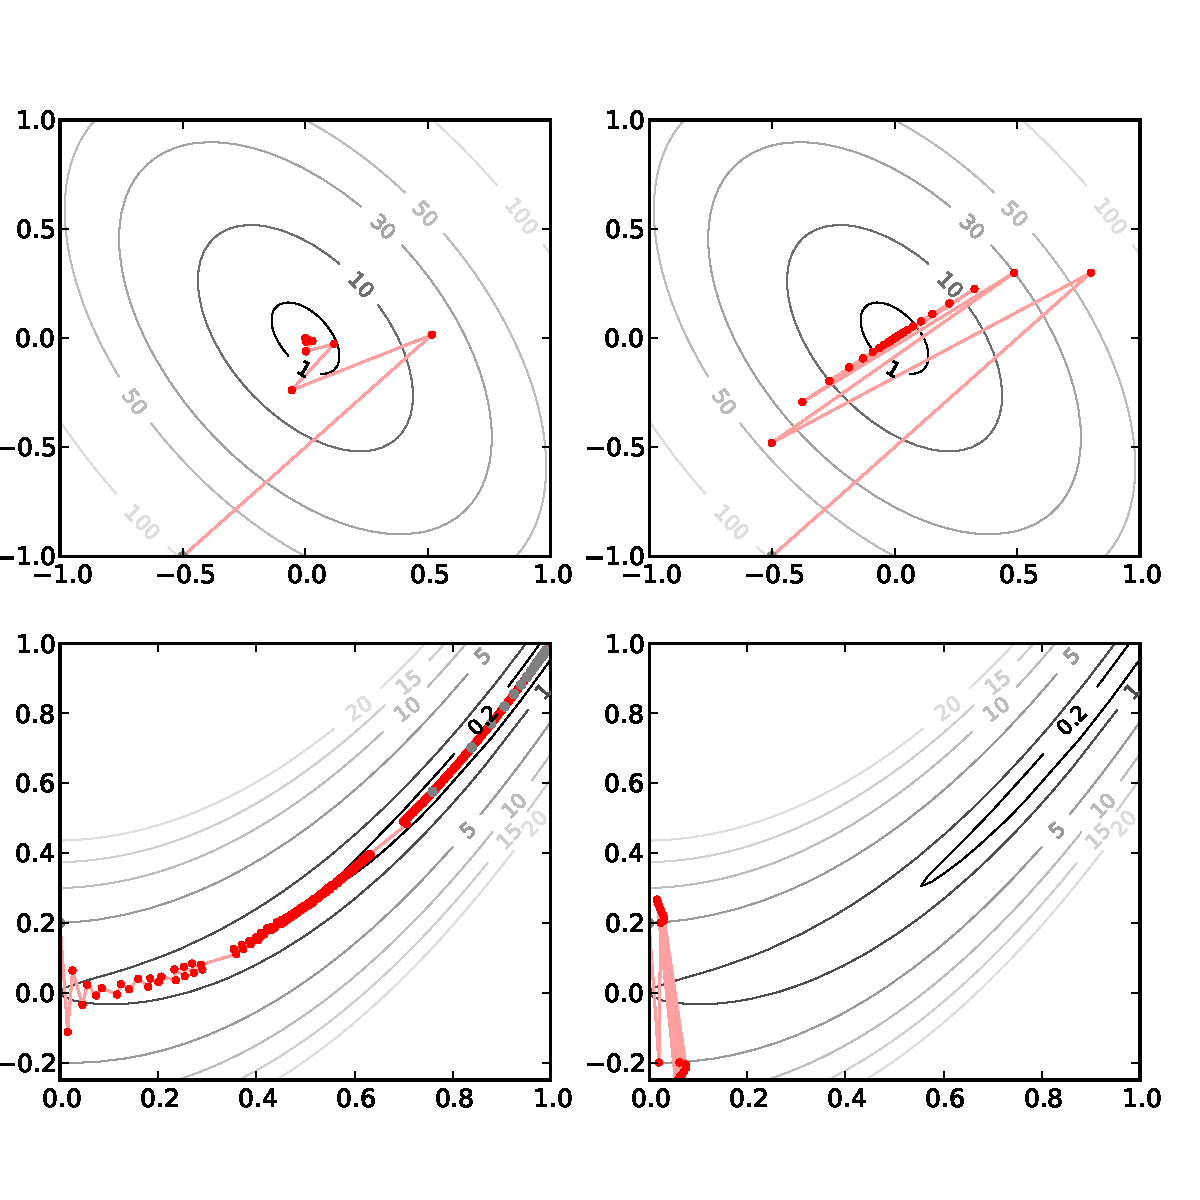
\includegraphics[width=\textwidth]{plots/steepestdescent}
  \caption{Verfahren des steilsten Abstiegs für eine quadratische
    Funktion (oben) und die Rosenbrockfunktion (unten). Links werden
    Armijo-Schrittweiten mit $\alpha=0,1$ und $\rho=0,5$, rechts eine
    konstante Schrittweite von $0,01$ verwendet. Die roten Punkte
    markieren die Iterierten $x^{(k)}$, die Höhenlinien illustrieren
    die zu optimierende Funktion. Für die quadratische Funktion
    konvergieren beide Verfahren gegen das Minimum bei $(0,\,0)$, und
    auch das Armijo-Verfahren wählt eine konstante Schrittweite von
    etwa $0,0078$. Durch diesen etwas kleineren Wert zielt das das
    schrittweitengesteuerte Verfahren weniger über das Minimum hinaus
    und braucht nur 11 statt 35 Schritte für 10 Stellen
    Genauigkeit. Bei der Rosenbrockfunktion benötigt das
    schrittweitengesteuerte Verfahren etwa 1700 Iterationen dafür.
    Jeder 200. Punkt ist im Graphen grau gefärbt, um die extrem
    langsame Konvergenz zu visualisieren. Für die konstante
    Schrittweite $0,01$ konvergiert das Verfahren gar nicht, wie die
    eingezeichneten ersten zehn Punkte zeigen.} \label{fig:armijo}
\end{figure}

Als Beispiel betrachten wir das Verfahren des steilsten Abstiegs für
zwei auf der Ebene definierte Funktionen. Die erste Funktion ist eine
quadratische Funktion
\begin{equation}
  \label{eq:quadgl}
  f(x, y) = 40 x^2 + 30(x + y)^2 + 20 y^2,
\end{equation}
die ihr Minimum bei $(0,0)$ hat, die zweite Funktion ist die
Rosenbrockfunktion\index{Rosenbrockfunktion}
\begin{equation}
  f_{\text{Rosenbrock}}(x, y) = (1-x)^2 + 100(y-x^2)^2.
\end{equation}
Diese hat ihr Minimum offenbar bei $(1,1)$, ist aber das
Optimierungsäquivalent zur Rungefunktion. Denn während das Minimum in
einem sehr steilen Tal liegt, ist der Gradient entlang der Talsohle
sehr flach. Die meist gierigen Optimierungsverfahren finden daher sehr
schnell in die Talsohle, kommen dort aber nur noch langsam ins Ziel,
da die Hauptabstiegsrichtung vorwiegend in die Talsohle statt
entlang dieser zeigt.

Abbildung~\ref{fig:armijo} zeigt die Anwendung des Verfahrens des
steilsten Abstiegs mit und ohne Schrittweitensteuerung auf die beiden
Funktionen und illustriert dabei die beiden Hauptschwächen des
Gradientenabstiegsverfahrens. Einerseits neigt es dazu, über das
Minimum hinauszuschießen, und sich dadurch langsam in das Minimum
einzupendeln. Dies lässt sich durch die Schrittweitensteuerung
begrenzen. Andererseits muss der steilste Abstieg nicht in Richtung
des Minimums zeigen, in diesem Fall neigt das Verfahren des steilsten
Abstiegs dazu, sich dem Minimum in Zick-Zack-Kurven mit sehr geringer
Schrittweite zu nähern.

Bei zu großer Schrittweite kann das Verfahren sogar gar nicht
konvergieren. Da von vornherein die maximale Ableitung meist nicht
bekannt ist, ist also eine Schrittweitensteuerung unerlässlich.

\subsection{\keyword{CG-Verfahren}}
\index{konjugierter Gradient}

Wir betrachten nun einen wichtigen Spezialfall, nämlich quadratische
Funktionen der Form
\begin{equation}
  \label{eq:cgfunktion}
  f(x) = \frac{1}{2}x^TAx - x^Tb
\end{equation}
mit positiv definiter Matrix $A\in\RR^{n,n}$.  Dies bedeutet, dass $A$
symmetrisch ist und $x^TAx>0$ für alle Vektoren $x\neq 0$ erfüllt,
etwa, weil alle Eigenwerte positiv sind.  Positiv definite Matrizen
treten zum Beispiel bei quantenmechanischen Rechnungen auf.

Für Funktionen der Form \eqref{eq:cgfunktion} gibt es ein iteratives
Verfahren, dass bei unbegrenzter Genauigkeit in spätestens $n$
Schritten gegen die exakte Lösung konvergiert. Dieses Verfahren ist
das konjugierte Gradienten-Verfahren (englisch conjugate gradient,
daher kurz auch CG-Verfahren).
Das Optimierungsproblem $\min f(x)$ kann dabei auch als Gleichung
aufgefasst werden, da
\begin{equation}
  Ax = b \quad\iff\quad x\;\text{minimiert}\;f(x) = \frac{1}{2}x^TAx - x^Tb.
\end{equation}
Daher wird das CG-Verfahren auch als effizienter
Gleichungslöser für positiv definite Matrizen behandelt.

Um das Minimum iterativ zu suchen, starten wir mit einem beliebigen
Startwert $x^{(0)}$ (zum Beispiel 0), und verfeinern die aktuelle
Näherung gemäß $x^{(k+1)} = x^{(k)} + \lambda^{(k)}d^{(k)}$ so, dass
wir uns dem Minimum nähern. Wie wir gesehen haben, ist der steilste
Abstieg, also in Richtung des negierten Gradienten $r^{(k)} =
b-Ax^{(k)}$, nicht ideal. Die Idee des CG-Verfahrens ist nun, die
Richtungen $d^{(k)}$ in gewisser Weise stets senkrecht zu einander zu
wählen, so dass Hin- und Herpendeln oder Zick-Zack-Kurse
ausgeschlossen sind. Tatsächlich wählt man die Abstiegsrichtungen
senkrecht in dem durch $A$ induzierten Skalarprodukt, also so, dass
$(d^{(i)}, d^{(k)})_A := \left(d^{(i)}\right)^TAd^{(k)}=0$ für $i\neq
k$. Man sagt auch, dass $d^{(i)}$ und $d^{(k)}$ $A$-konjugiert sind,
daher der Name des Verfahrens.

\begin{figure}
  \centering
  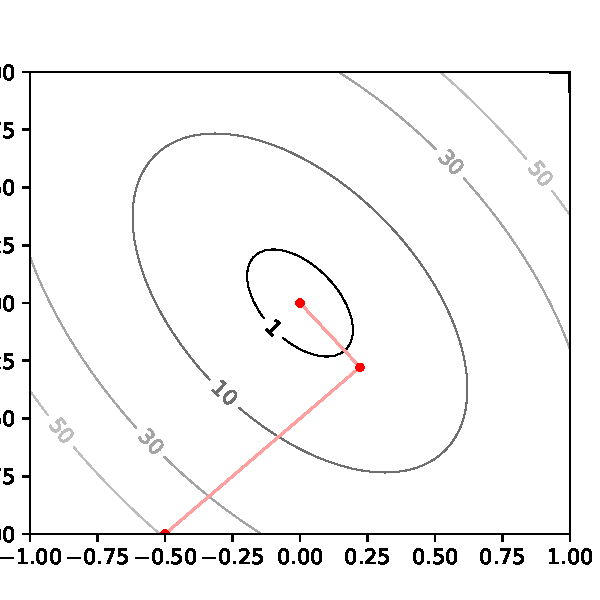
\includegraphics[width=0.5\textwidth]{plots/cg}
  \caption{CG-Verfahren für die quadratische Funktion aus
    \eqref{eq:quadgl}. Die Höhenlinien stellen die zu optimierende
    quadratische Funktion dar, die roten Punkte markieren die
    Iterierten des CG-Verfahrens, das in nur 2 Schritten konvergiert.}
  \label{fig:cg}
\end{figure}

Die $d^{(k)}$ werden konstruiert, indem die
Gradientenabstiegsrichtungen $r^{(k)}$ mit Hilfe des
Gram-Schmidt-Verfahrens zueinander senkrecht bezüglich
$(\cdot,\cdot)_A$ gemacht werden. Dabei muss aufgrund der Wahl der
Richtungen $d^{(k+1)}$ nur senkrecht zu $d^{(k)}$ gemacht werden, zu
den anderen bisherigen Richtungen steht $d^{(k+1)}$ dann automatisch
senkrecht. Der Vorfaktor kann dabei vereinfacht werden:
\begin{equation}
  \frac{(r^{(k+1)}, d^{(k)})_A}{(d^{(k)}, d^{(k)})_A}
  = -\frac{\left(r^{(k+1)}\right)^Tr^{(k+1)}}{\left(r^{(k)}\right)^Tr^{(k)}}.
\end{equation}

Die Schrittweite kann bei einer quadratischen Funktion so bestimmt
werden, das $\lambda$ die Funktion entlang der Richtung $d$, also
\begin{equation}
  \frac{1}{2}(x+\lambda d)^TA(x+\lambda d) - b^T(x+\lambda d)
  =  \frac{1}{2}x^TAx - b^Tx + \lambda d^T(Ax - b) + \frac{1}{2}\lambda^2 d^TAd,
\end{equation}
minimiert. Es ergibt sich
\begin{equation}
  \lambda^{(k)}  =  \frac{\left(d^{(k)}\right)^Tr^{(k)}}{\left(d^{(k)}\right)^TAd^{(k)}}.
\end{equation}

Zusammengefasst ergibt sich das CG-Verfahren in Python als
\lstinputlisting[firstline=10]{cg.py}%
Das Verfahren bricht ab, wenn $\norm{r^{(k)}} <$ \argd{tol}, anstatt
stur $n$ Schritte zu berechnen, da durch numerische Ungenauigkeiten
unter Umständen 1-2 zusätzlich Schritte nötig werden können. Umgekehrt
können natürlich auch weniger Schritte notwendig sein, wenn der
Startwert günstig liegt.

Abbildung~\ref{fig:cg} illustriert das CG-Verfahren an der selben
quadratischen Funktion, für die das schrittweitengesteuerte
Gradientenabstiegsverfahren 11 Schritte brauchte, um 10 Stellen
Genauigkeit zu erreichen. Das CG-Verfahren hingegen konvergiert in nur
zwei Schritten auf Maschinengenauigkeit, also etwa 17 Stellen.

Da das Verfahren auch als Gleichungslöser sehr gute Eigenschaften hat
und wegen der überwiegenden Skalar- und Matrix-Vektorprodukte auch
sehr einfach auf dünnbesetzten Matrizen eingesetzt werden kann, ist es
eines der meist genutzten Verfahren. Daher gibt es natürlich auch eine
SciPy-Implementation, \scipy{scipy.sparse.linalg.cg(A, b)}.

\subsection{Nebenbedingungen und Straffunktionen}
\index{Straffunktion}
\index{Penalty function}

Mit dem Verfahren des steilsten Abstiegs und den Armijo-Schrittweiten
haben wir ein stabiles und meist schnell konvergierendes Verfahren, um
lokal freie Minima zu suchen. Was aber kann man tun, wenn zusätzlich
noch Nebenbedingungen gegeben sind? Wir suchen nun also $\min_{x\in M}
f(x)$, wobei die zulässige Menge
\begin{equation}
  M=\left\{ x | g_i(x)\ge 0,\,i=1(1)m \right\}
\end{equation}
ist. Bekannte Verfahren sind etwa die sequenzielle quadratische
Programmierung (SQP) oder das Verfahren von Gill und
Murray~\cite{gill78a}. Hier lernen wir einen anderen, physikalisch
motivierten Ansatz kennen.

Dazu setzen wir voraus, dass nicht nur die zu minimierende Funktion
$f:\RR^n\to\RR$ stetig differenzierbar ist, sondern auch die
Funktionen $g_i:\RR^n\to\RR$, die die Nebenbedingungen
definieren. Wäre nun $g_i(x)=-\infty$ für alle $x\notin M$ oder
zumindest kleiner als das gesuchte Minimum von $f$ in $M$, so wäre
\begin{equation}
  \min_{x\in M} f(x) = \min_{x\in\RR^n} f(x) + \sum_{i=1}^m \min(0,
  g_i(x))^2.
\end{equation}
In der Praxis ist einerseits $g_i(x)$ im Allgemeinen endlich,
andererseits kennen wir aber auch kein Verfahren, um eine höchst
unstetige Funktion zu minimieren. Wenn wir uns die Nebenbedingungen
aber als Banden vorstellen, über die ein iterativer Algorithmus nicht
hinausschreiten darf, könnte man diese zunächst weicher gestalten, so
dass der Algorithmus den zulässigen Bereich etwas verlassen kann, und
dann die Banden mit der Zeit immer härter gestalten, so dass der
Algorithmus schließlich in den zulässigen Bereich gedrückt
wird. Befindet sich das Minimum über $M$ am Rand von $M$, wird die
gefundene Näherungslösung daher immer minimal außerhalb von $M$
liegen. Ist dies ein Problem, etwa weil $f$ außerhalb $M$ nicht
ausgewertet werden kann, kann man stattdessen auf Barrieremethoden
ausweichen, bei denen die Banden bereits innerhalb von $M$ beginnen
und am Rand von $M$ singulär sind.

Beim Straffunktionsverfahren minimieren wir also die modifizierte
Funktion
\begin{equation}
  \label{eq:penalty}
  q_{\sigma}(x) = f(x) + \sum_{i=1}^m \min(0,
  \sigma g_i(x))^2.
\end{equation}
Der hintere Teil $p_{\sigma}(x) = \sum_{i=1}^m \min(0, \sigma
g_i(x))^2$ wird dabei Straffunktion (Penalty function)
genannt, weil er Punkte außerhalb des zulässigen Bereichs mit höheren
Funktionswerten bestraft.

\begin{figure}
  \centering
  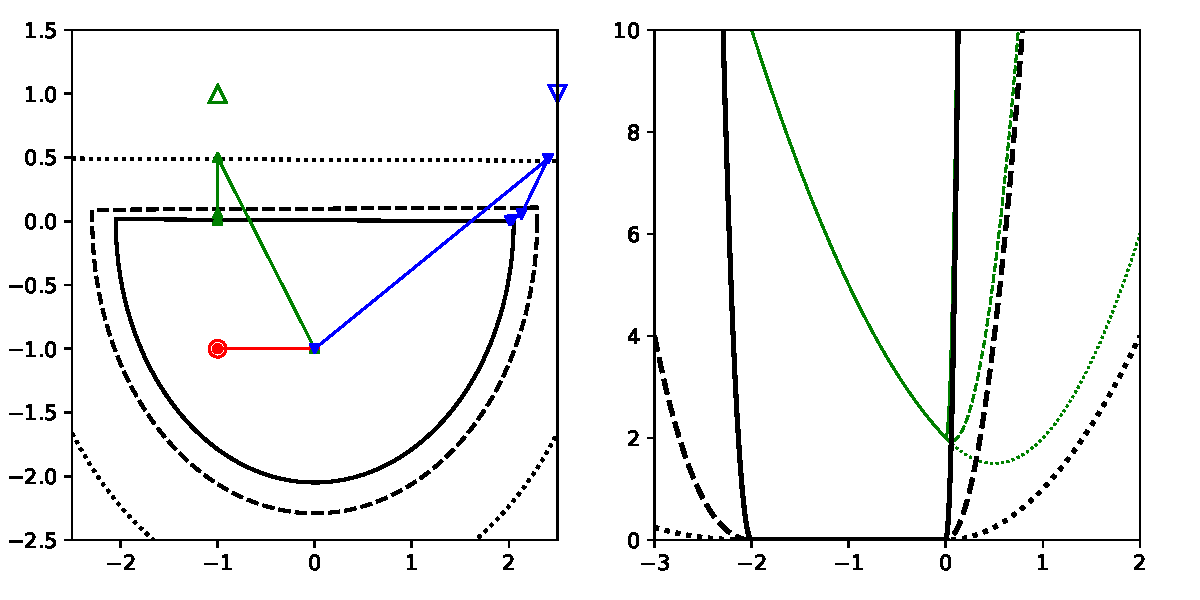
\includegraphics[width=\textwidth]{plots/penalty}
  \caption{Straffunktionsverfahren für einen Halbkreis. Die
    durchgezogenen, gestrichelten, und gepunkteten Linien markieren
    die Isolinien $p_{\sigma}(x)=\nicefrac{1}{2}$ in den Schritten 1,2
    und 5. Minimiert wird jeweils der Abstand zum den mit offenen
    Symbolen markierten drei Punkten. Der rote Kreis liegt im inneren,
    das Verfahren braucht nur einen Aufruf des freien Optimierers. Für
    die grünen und blauen Dreiecke sind jeweils mehrere Aufrufe nötig,
    wobei das blaue, nach unten zeigende Dreieck so gewählt ist, dass
    das Minimum in der Ecke liegt. Im rechten Graphen sind die
    Straffunktionen entlang der $y$-Achse, also $p_{\sigma}(0,y)$, für
    dieselben Schritte gezeigt. Dünner grün sind die korrespondieren
    Zielfunktionen $q_{\sigma}(0,y)$ eingezeichnet.}
  \label{fig:penalty}
\end{figure}

Um das Minimum zu finden, starten wir mit recht kleinem
$\sigma_0>0$. Auf $q_{\sigma_0}$ wenden wir dann ein
Optimierungsverfahren für freie Optimierung an, etwa das Verfahren des
steilsten Abstiegs mit Schrittweitensteuerung. Aufgrund der
Konstruktion ist der Gradient von $q_{\sigma}$ recht einfach zu berechnen:
\begin{equation}
  \nabla q_{\sigma}(x) = \nabla f(x) + \sum_{i=1}^m 2\sigma^2\min(0,
  g_i(x))\nabla g_i(x).
\end{equation}

Sinnvollerweise wählt man einen Startpunkt im Inneren von $M$. Ist im
gefundenen, freien Minimum von $q$ bereits $g_i(x)\ge - \tau$ mit
gewünschter Toleranz $\tau$ erfüllt, ist das Minimum gefunden, und
liegt sehr wahrscheinlich im Inneren vom $M$. Ansonsten wird
$\sigma_k$ erhöht und erneut die Minimierung gestartet, allerdings
naheliegenderweise mit dem bereits gefundenen Minimum als
Startwert. Die Lage des Minimums ändert sich dabei, da ja wegen der
Abbruchbedingung wenigstens eine Nebenbedingung noch nicht erfüllt
war, und sich diese durch die Änderung von $\sigma_k$ ändert. Solange
danach $g_i(x)\ge - \tau$ nicht erreicht ist, passen wir $\sigma_k$ an
und iterieren weiter.
$\sigma_k$ kann auf verschiedene Weisen gewählt werden, es muss nur
$\sigma_k\to \infty$ für $k\to\infty$ gelten. Eine Möglichkeit ist
etwa $\sigma_k=k^a$ , wobei man $a>1$ nicht zu groß wählen sollte, zum
Beispiel $a=2$.

Abbildung~\ref{fig:penalty} illustriert das Verfahren am Beispiel
einer Abstandsminimierung zu einem Halbkreis. Wir suchen also
\begin{equation}
  \min_{x\in M} \norm{x - p}_2\quad\text{mit}\;
  M = \{ (x,y)\,|\, g_i(x,y) \ge 0, i=1,2 \}
\end{equation}
mit
\begin{equation*}
  g_1(x, y) = 4 - x^2-y^2\quad\text{und}\; g_2(x,y) = -10y.
\end{equation*}
Dies entspricht offenbar $\norm{(x,y)}_2\le 2$ und $y<0$, also dem
Halbkreis. Im Beispiel werden drei verschiedene Punkte betrachtet und
mit Hilfe des Straffunktionsverfahrens und einem
schrittweitengesteuerten Gradientenverfahren der nächste Punkt im
Halbkreis gesucht. Der Straffaktor $\sigma$ wurde als $0,1\,k^2$
gewählt, mit $k=1,2,\ldots$ der Iterationsschritt. $p=(-1,\,-1)$ liegt
selber im Inneren des Halbkreises und wird daher gleich im ersten
Optimierungsschritt als nächster Punkt gefunden. Für die beiden
anderen Punkte, $p=(-1,\,1)$ und $p=(2,5,\,1)$, sind nur die Gerade
beziehungsweise beide Ungleichungen gleichzeitig aktiv; auch hier
werden die nächsten Punkte am Rand des Halbkreises innerhalb weniger
Iterationen gefunden. Auf der rechten Seite sieht man, dass die
Straffunktionen sehr steil werden. Daher ist eine
Schrittweitensteuerung hier besonders wichtig.

\section{Lineare Programme und Simplexalgorithmus}
\index{lineares Programm}
\index{Simplexalgorithmus}

Wie wir in der Einleitung gesehen hatten, führt die lineare Regression
mit Maximumsnorm zu einem ganz anderen Typ von Problem, bei dem die
Zielfunktion linear ist. Dadurch liegt das Minimum notwendigerweise
auf dem Rand der zulässigen Menge. Sind zusätzlich noch die
Nebenbedingungs(un-)gleichungen linear
(vgl. Abbildung~\ref{fig:simplex}), spricht man von einem
\emph{linearen Programm}. Programm hat hier also erst einmal nichts
mit Computern zu tun. Solche linearen Programme spielen auch in der
Optimierung von Wirtschaftsprozessen eine wichtige Rolle ("`Operations
research"'), da Gewinn und produzierte Mengen bei unverändertem Preis
linear von einander abhängen.

\begin{figure}
  \centering
  \begin{tikzpicture}[x=8em,y=8em]
    \draw[->] (-0.1,0) -- (1.2,0);
    \draw[->] (0,-0.1) -- (0,1.2);

    % zulässiger Bereich
    \draw (1,0) -- (0,1) ;
    \fill[pattern=north east lines,rotate around={135:(1,0)}] (1,0) rectangle +(1.414,-0.1) ;
    \fill[pattern=north east lines] (0,0) rectangle +(1,-0.1) ;
    \fill[pattern=north east lines] (0,0) rectangle +(-0.1,1) ;

    % Zielfunktion
    \pgfmathsetmacro{\gradx}{-0.3}
    \pgfmathsetmacro{\grady}{ 0.4}
    \pgfmathsetmacro{\perpx}{\grady}
    \pgfmathsetmacro{\perpy}{-\gradx}

    \draw[very thick,->=triangle 45] (0.5,0.2) -- +(\gradx,\grady);

    % Isolinien
    \foreach \l in {0,0.2,0.4,...,0.8} {
      \pgfmathsetmacro{\ll}{(1-\l)/(\perpx+\perpy)}     
      \draw (0, \l) -- (\ll*\perpx,\l+\ll*\perpy);
    }

    \foreach \l in {0.2,0.2,0.4,...,0.8} {
      \pgfmathsetmacro{\ll}{(1-\l)/(\perpx+\perpy)}     
      \draw (\l, 0) -- (\l + \ll*\perpx, \ll*\perpy);
    }

    % Minimum
    \filldraw (1, 0) circle (0.04);

  \end{tikzpicture}
  \hspace{4em}
  \begin{tikzpicture}[x={(4em,2em)},y={(4em,-2em)},z={(0em,5em)}]
    \draw (xyz cs:x=-.1) -- (xyz cs:x=0);
    \draw (xyz cs:y=-.1) -- (xyz cs:y=0);
    \draw (xyz cs:z=-.1) -- (xyz cs:z=0);

    \draw[thick,->] (xyz cs:x=0) -- (xyz cs:x=1.3) node[right] {$x$};
    \draw[thick,->] (xyz cs:y=0) -- (xyz cs:y=1.3) node[right] {$y$};
    \draw[thick,->] (xyz cs:z=0) -- (xyz cs:z=1.3) node[above] {$z$};

    \draw[color=green,fill=green!80!white,opacity=0.5]
    (xyz cs:z=1) -- (xyz cs:x=1) -- (xyz cs:y=1) -- cycle;
    \draw[color=green]
    (xyz cs:z=1) -- (xyz cs:x=1) -- (xyz cs:y=1) -- cycle;

    \draw[color=green]
    (xyz cs:z=1) circle (0.02)
    (xyz cs:x=1) circle (0.02)
    (xyz cs:y=1) circle (0.02);

    \draw[color=red]
    (xyz cs:z=1,x=0.5) -- (xyz cs:z=0.2,y=0.8);

    \draw[color=red]
    (xyz cs:z=1,x=0.5)   circle (0.02)
    (xyz cs:z=0.2,y=0.8) circle (0.02);
  \end{tikzpicture}
  \caption{Links: Illustration eines linearen Programms. Die
    Nebenbedingungen sind $x\ge 0$, $y\ge 0$ und $1 - x \ge y$; die
    Schraffuren markieren den ausgeschlossenen Bereich. Der Pfeil
    deutet den Gradienten der Zielfunktion an, die Linien im
    zulässigen Bereich sind Isolinien des Potentials. Hier findet sich
    das Minimum in der mit einem Punkt markierten rechten unteren
    Ecke. Rechts: Dreidimensionaler zulässiger Bereich $x\ge 0$ mit
    weiterer Nebenbedingung. Ist eine Nebenbedingung $a^Tx=b$ gegeben,
    so sind nur Punkte mit Koordinaten $\ge 0$ aus dieser Ebene
    zulässig, also aus dem grünen Dreieck. Die Projektion dieses
    Dreiecks in die $xy$-Ebene entspricht dem zulässigen Bereich in
    der linken Illustration. Die Ecken lassen sich durch die Menge der
    Koordinaten, die nicht Null sind, vollständig beschreiben. Die
    unterste Ecke etwa hat nur $y$ aktiv, die obere $z$. Sind zwei
    Nebenbedingungen gegeben, so ist die resultierende zulässige Menge
    eine Gerade (hier rot eingezeichnet). Die Ecken werden nun durch
    zwei aktive Koordinaten beschrieben, hier $y$ und $z$ für die
    vordere Ecke, und $x$ und $z$ für die hintere.}
  \label{fig:simplex}
\end{figure}

Lineare Programme können in einer Vielzahl von Formen definiert
werden, wir betrachten hier die Normalform
\begin{equation}
  \label{eq:simplexprob}
  \min c^Tx \quad\text{unter den Nebenbedingungen}\; x\ge 0,\;Ax=b
\end{equation}
mit $c\in\RR^n$, $A\in\RR^{m,n}$ und $b\in\RR^{m}$. Die Anzahl $m$ der
Gleichungsbedingungen ist dabei nicht festgelegt. Da $x$ ein Vektor
ist, bedeutet $x\ge 0$ einfach, dass alle Komponenten größer als Null
sein sollen. Alle linearen Nebenbedingungen lassen sich so
formulieren, eventuell unter Zuhilfenahme von weiteren Variablen.

Betrachten wir zwei Beispiele. Die in der Abbildung~\ref{fig:simplex}
gegebene Nebenbedingung $1 - x \ge y$ ist nicht von der obigen
Form. Wir führen deswegen eine neue Variable $z=1-x-y$ ein, die dann
$z\ge 0$ erfüllen muss. Wir erhalten die Normalform mit $c'=(c_0, c_1,
0)$, da $z$ ja nicht zur Zielfunktion beiträgt, sowie $A=(1,\,1,\,1)$
und $b=1$. Abbildung~\ref{fig:simplex} rechts zeigt den resultierenden
zulässigen Bereich im dreidimensionalen Raum.

Auch das Problem
\begin{equation}
  \min_v (0,\ldots,\,0,\,1)^T v\quad\text{unter der Bedingung}\;
  \begin{pmatrix}
    A & e\\
    -A & e
  \end{pmatrix} v \ge
  \begin{pmatrix}
    b\\
    -b
  \end{pmatrix},
\end{equation}
das sich bei der linearen Regression mit Maximumsnorm ergibt
(vgl.~\eqref{eq:chebyshevappr}), ist nicht in Normalform. Zum einen
müssen wir die Nebenbedingungsungleichungen in Gleichungen
transformieren. Dazu führen wir einfach eine Schattenvariable
$z_i=a_i^Tv - b_i$ pro Ungleichung $a_i^Tv\ge b_i$ ein. Dann ist
$z_i\ge 0$ offenbar äquivalent zur ursprünglichen Ungleichung. Zum
anderen sind aber die Variablen $v$ frei, während wir voraussetzen,
dass $v\ge 0$. Um dies zu beheben, teilen wir jede Variable in $v=v_+
- v_-$ mit $v_\pm\ge 0$ auf und ergänzen $A$ und $c$ entsprechend. Das
ergibt die äquivalente Aufgabe%
{\samepage\vspace{0.2em}% für die TikZ-Deko
  \begin{equation}
    \label{eq:chebyshevapprnf}
    \min_x (\tikzlabel{vpl}0,\ldots,\,0,\,1\tikzlabel{vpr},
    \tikzlabel{vml}0,\ldots,\,0,\,-1\tikzlabel{vmr},
    \tikzlabel{zl}0,\ldots,\,0\tikzlabel{zr})^T v
  \end{equation}
  \begin{tikzpicture}[overlay, remember picture]
    \draw[decorate,decoration=brace] ($(vpl) + (0,1em)$) --
    node[above] {$v_+$} ($(vpr) + (0,1em)$);
    \draw[decorate,decoration=brace] ($(vml) + (0,1em)$) --
    node[above] {$v_-$} ($(vmr) + (0,1em)$);
    \draw[decorate,decoration=brace] ($(zl) + (0,1em)$) --
    node[above] {$z$} ($(zr) + (0,1em)$);
  \end{tikzpicture}}
mit der neuen Variablen $x=(v_+,v_-,z)$ und den Nebenbedingungen $x\ge 0$
und
{\samepage\vspace{0.2em}% für die TikZ-Deko
\begin{equation*}
  \begin{pmatrix}
    \tikzlabel{vpl}A  & e\tikzlabel{vpr} & 
    \tikzlabel{vml}-A & -e\tikzlabel{vmr} &
    \tikzlabel{zl} -I & 0\tikzlabel{zr}\\
    -A & e &  A & -e & 0 & -I
  \end{pmatrix}
  x =
  \begin{pmatrix}
    b\\
    -b
  \end{pmatrix}.
\end{equation*}
\begin{tikzpicture}[overlay, remember picture]
  \draw[decorate,decoration=brace] ($(vpl) + (0,1em)$) --
  node[above] {$v_+$} ($(vpr) + (0,1em)$);
  \draw[decorate,decoration=brace] ($(vml) + (0,1em)$) --
  node[above] {$v_-$} ($(vmr) + (0,1em)$);
  \draw[decorate,decoration=brace] ($(zl) + (0,1em)$) --
  node[above] {$z$} ($(zr) + (0,1em)$);
\end{tikzpicture}}

Wie können wir Aufgabe \eqref{eq:simplexprob} lösen? Sofern die
zulässige Menge beschränkt ist, beschreiben die Nebenbedingungen immer
einen Polyeder. Man kann nun zeigen, dass sich ein Optimum immer in
einer der Ecken dieses Polyeders befindet. Der
\emph{Simplexalgorithmus} besucht nacheinander die Ecken des
Polyeders, wobei die Zielfunktion ständig kleiner wird. Da es nur
endliche viele Ecken gibt, findet der Algorithmus das Minimum
irgendwann. Es gibt pathologische Beispiele, in denen der Algorithmus
alle Ecken absuchen muss. Im Allgemeinen konvergiert der
Simplexalgorithmus aber schnell.

Die Methode zerfällt dabei in zwei Phasen. In der ersten Phase muss
eine gültige Ecke bestimmt werden, in der zweiten Phase müssen wir
dann von einer gültigen Ecke aus eine neue, benachbarte Ecke mit
niedrigerer Zielfunktion finden. Wir beginnen mit der Beschreibung der
zweiten Phase, da die die erste Phase die zweite Phase benutzt, um ein
erweitertes Problem zu lösen, dass erlaubt, eine erste Ecke zu finden.

\subsubsection*{Phase II}

Wir nehmen an, dass die Matrix $A$ maximalen Zeilenrang hat, also alle
doppelten Gleichung eliminiert wurden; dies wird später die erste
Phase übernehmen.  Außerdem sei $x$ eine Ecke des Polyeders.

Wie stellen wir diese Ecke dar? Abbildung~\ref{fig:simplex}
illustriert, dass eine Ecke einfach durch die Menge der aktiven, also
von Null verschiedenen Koordinaten beschrieben werden kann. Da wir
angenommen haben, dass $A\in\RR^{m,n}$ linear unabhängige Zeilen hat,
beschreibt $Ax=b$ einen $n-m$-dimensionalen Unterraum, dessen Ecken
jeweils $m$ aktive Koordinaten haben.

Sei $B=\{j_1,\ldots,k_m\}$ die Menge der in der aktuellen Ecke aktiven
Koordinaten, die sogenannten Basiskoordinaten, und
$N=\{1,\ldots,n\}\backslash B$ die Menge der
Nichtbasiskoordinaten. $A_B = (a_{j_1},\ldots,a_{j_m})\in\RR^{m,m}$
sei die zu den Basisvariablen $x_B = (x_{j_i})_i\in\RR^m$ gehörende
Teilmatrix, sowie $A_N$ analog die zu den Nichtbasisvariablen
gehörende Teilmatrix. Dann gilt $x_N=0$ und damit $A_Bx_b = b$.
Der Zielfunktionswert in $x$ ist deshalb
\begin{equation}
  c^Tx = c_B^Tx_B = c_BA_B^{-1}b.
\end{equation}
Wir betrachten nun eine beliebigen anderen Punkt $u\in M$, also $u\ge
0$ und $Au=A_Bu_B + A_Nu_N = b$. Dann ist
\begin{equation}
  \label{eq:simplexub}
  u_b = A_B^{-1}(b - A_Nu_N) = x_B - A_B^{-1}A_Nu_N
\end{equation}
und damit
\begin{equation}
  c^Tu = c_B^T(x_B - A_B^{-1}A_Nu_N) + c_N^Tu_N = c^Tx +
  \underbrace{\left(c_N - A_N^T\left(A_B^{-1}\right)^Tc_B\right)^T}_{r}u_n.
\end{equation}
Da $u_N\ge 0$ ist, kann die Zielfunktion nur verkleinert werden, wenn
eine Komponente $r_s < 0$ ist. Ist dies nicht der Fall, haben wir also
unser Optimum gefunden.

Sei nun also $s$ so gewählt, dass $r_s< 0$ minimal. Dann können wir
unser Ergebnis verbessern, indem wir $u_s>0$ wählen, aber alle
anderen Elemente von $u_N$ weiterhin bei 0 belassen. Wir nehmen also
$s$ in die Basiskoordinaten $B$ auf. Damit diese eine Basis bleiben,
müssen wir nun noch sehen, welche Gleichung dafür herausfällt. Aus
\eqref{eq:simplexub} folgt, dass $u_B = x_B - u_s A_B^{-1}a_s$.  Auch
im neuen Punkt muss aber $u_B\ge 0$ gelten, daher können wir $u_N$ nur
so groß wählen, bis für die erste Basisvariable $x_t= u_s
(A_B^{-1}a_s)_t$ gilt. Dann gilt $u_t=0$, \dh diese Basisvariable
geht in die Nichtbasis über.
Wir suchen also
\begin{equation}
  u_s = \min \left\{\frac{x_{j_k}}{(A_B^{-1}a_s)_k} | k\in B,
      (A_B^{-1}a_s)_k > 0\right\} =:
  \frac{x_{j_t}}{(A_B^{-1}a_s)_t}
\end{equation}
Sind dabei alle $(A_B^{-1}a_s)_k < 0$, so dass das Minimum gar nicht
existiert, können wir $u_B$ unbegrenzt groß machen. Also ist der
zulässige Bereich unbeschränkt, und wir müssen abbrechen, da die
Funktion beliebig klein werden kann und also kein Minimum hat.

Wir tauschen nun in der Basis $B$ die gefundene beschränkende
Basisvariable  $j_t$ durch $s$ aus und erhalten die
neue Basis $B'$. In $A_B$ wird dabei einfach die Spalte $t$ durch
$a_s$ ersetzt, also
\begin{equation}
  A_{B'} = A_B + (a_s - a_{j_t})e_t^T
\end{equation}
Für die Rechnungen benötigen wir aber $A_B^{-1}$, dass wir allerdings
auch mit einer Rang-1-Formel anpassen können. Die
Sherman-Morrison-Formel liefert
\begin{equation}
  \label{eq:simplexex}
  A_{B'}^{-1} = A_{B}^{-1} - \frac{A_B^{-1}a_s - e_t}{(A_B^{-1}a_s)_t}
  \left(e_t^TA_{B}^{-1}\right).
\end{equation}

\subsubsection*{Phase I}

Wie können wir nun eine zulässige erste Lösung mit zugehörigem
Basissatz und $A_B^{-1}$ finden? Die Idee ist, zunächst die Matrix
noch einmal stark zu erweitern, sodass eine gültige Ecke einfach zu
finden ist, aber nur die Ecken des ursprünglichen zulässigen Bereichs
optimal. Phase kann dann genutzt werden, um eine solche Ecke zu finden.

Dazu betrachten wir das neue Problem
{\samepage\vspace{0.2em}\begin{equation}
  \min_z (\tikzlabel{xl}0,\ldots,\,0,\tikzlabel{xr},
  \tikzlabel{yl}1,\ldots,\,1\tikzlabel{yr})^Tz
\end{equation}
\begin{tikzpicture}[overlay, remember picture]
  \draw[decorate,decoration=brace] ($(xl) + (0,1em)$) --
  node[above] {$x$} ($(xr) + (0,1em)$);
  \draw[decorate,decoration=brace] ($(yl) + (0,1em)$) --
  node[above] {$y$} ($(yr) + (0,1em)$);
\end{tikzpicture}}
mit der Variablen $z=(x,\,y)\in\RR^{n+m}$ und den Nebenbedingungen $z\ge 0$
und
\begin{equation*}
  \begin{pmatrix}
    \tilde{A} & I 
  \end{pmatrix}
  z =
  \tilde{b}
\end{equation*}
Dabei sind die $i$-ten Zeilen von $\tilde{A}$ und $\tilde{b}$
identisch mit denen von $A$ und $b$, nur werden die Vorzeichen
getauscht, falls $b_i<0$. Dies ändert die Lösungen des
Gleichungssystems nicht, aber es gilt $\tilde{b}\ge 0$. Durch die
Identität in den hinteren Spalten hat diese Matrix unabhängig vom
ursprünglichen $A$ maximalen Zeilenrang.

Sofern die ursprüngliche zulässige Menge nicht leer war, ist das
Minimum dieser Zielfunktion offenbar Null, nämlich dann, wenn alle
$y=0$ sind. Außerdem kennen wir einen zulässigen Punkt des neuen
Problems, nämlich $(0,\,\tilde{b})$, und die zugehörige Matrix
$A_B=I$.  Daher kennen wir auch $A_B^{-1}=I$, das im Folgenden dann
nur angepasst werden muss. Wir können also die Phase I des
Simplexalgorithmus unmittelbar auf diese Matrix anwenden.

Findet der Simplex-Algorithmus nun ein Minimum, dass von Null
verschieden ist, ist offenbar die ursprüngliche zulässige Menge leer
gewesen, und wir müssen abbrechen. Ist das Minimum hingegen Null und
alle $y=0$, also in der Nichtbasis, so haben wir unseren Startwert für
die Phase II gefunden. Es kann allerdings auch passieren, dass noch zu
$y$ gehörige Indizes $j_t>n$ in der Basis vorkommen. Dann müssen wir
eine echte Koordinate $s<n$ finden, die mit $j_t$ getauscht werden
kann. Dazu suchen wir ein $s$ mit $A_B^{-1}a_s)_t\neq 0$, so dass wir
wieder unsere Austauschformel \eqref{eq:simplexex} auf die Spalten $s$
und $j_t$ anwenden können. Finden wir kein solches $s$, dann kann man
zeigen,dass die ursprüngliche Matrix linear abhängige Zeilen hatte. In
diesem Fall wird die $j_t-n$-te Zeile gestrichen. In $A_B^{-1}$ müssen
entsprechend die $j_t-n$-te Spalte und $t$-te Spalte eliminiert
werden.

Quellcode~\ref{lst:simplex} zeigt eine Implementation des
Simplexverfahrens in Python.

\subsubsection{Beispiel: Polynomapproximation}
\index{Polynomapproximation}

\begin{figure}[t]
  \centering
  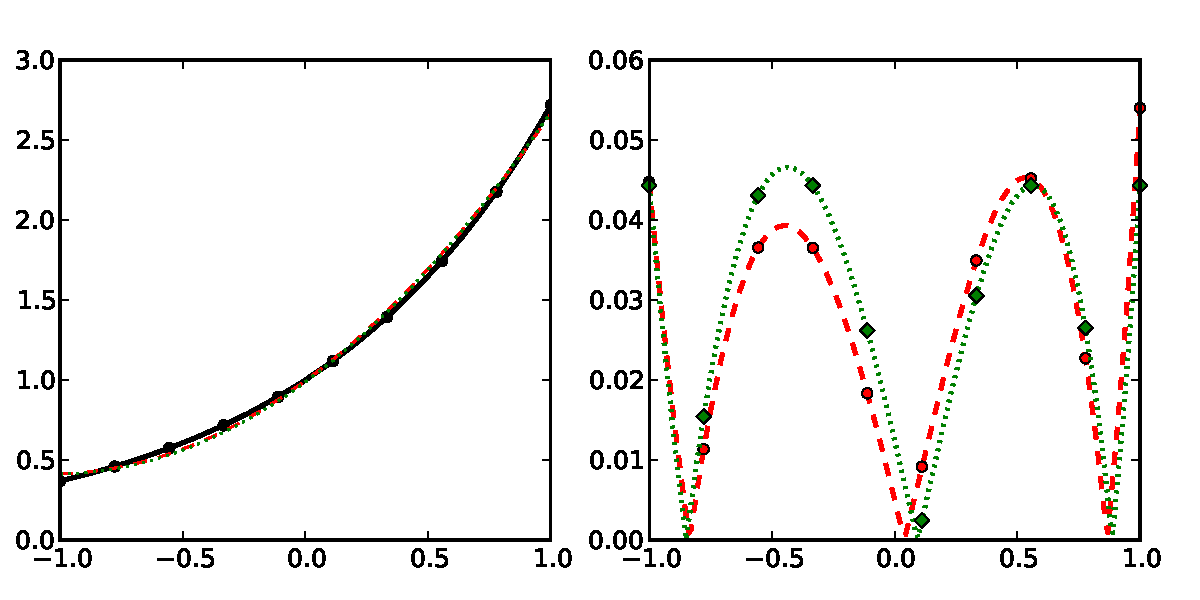
\includegraphics[width=\textwidth]{plots/qr_simplex_example}
  \caption{Polynomapproximation von $\exp(x)$ (durchgezogene Kurve
    links) im Bereich $[-1,1]$. Die Punkte markieren die 10
    Stützstellen. Anders als bei der Interpolation ist hier nur ein
    Polynom zweiten Grades gesucht, dass $\exp(x)$ an den gegebenen
    Stützstellen möglichst gut annähern soll. Die rot gestrichelte
    Lösung ist dabei die Lösung der kleinsten Quadrate, die grün
    gepunktete Lösung die mit minimaler maximaler Abweichung. Im
    rechten Graphen sind die absoluten Abweichungen zwischen den
    beiden Polynomnäherungen und $\exp(x)$ gezeigt. Die zweite Lösung
    erkauft sich eine niedrigere Abweichung am rechten Rand durch
    deutliche höhere Abweichung zwischen $-0,8$ und $0$. Die maximalen
    Fehler sind dadurch gleichmäßig über das Intervall verteilt.}
  \label{fig:polyapprox}
\end{figure}

Als Beispiel für den Simplexalgorithmus und gleichzeitig noch einmal
die Pseudoinversen soll das Beispiel der Polynomapproximation
dienen. Gegeben Stützstellen $x_i, y_i$, $i=1(1)m$, suchen wir ein
Polynom $p(x)=\sum_{i=0}^{n-1} c_ix^i$, so dass
\begin{equation}
  \norm{p(x_i) - y_i} = \norm{A c - b}
\end{equation}
minimal ist. Die Matrix $A$ ist dabei analog \eqref{eq:interpol} definiert:
\begin{equation}
  A=
  \begin{pmatrix}
    1 & x_1 & x_1^2 & \ldots & x_1^{n-1}\\
    \vdots & \vdots & & \vdots \\
    1 & x_m & x_m^2 & \ldots & x_m^{n-1}\\
  \end{pmatrix}
\end{equation}
und $b=(y_i)_i$. Ist $m=n$ und die $x$-Koordinaten der Stützstellen
$x_i$ paarweise verschieden, fällt die Polynomapproximation mit der
Interpolation zusammen, da der minimale Fehler $0$ offenbar durch das
eindeutige interpolierende Polynom erreicht wird.

Anders als bei der Interpolation wählt man aber im Allgemeinen $m\gg
n$, das Polynom kann also nicht alle Stützstellen passieren, und wird
im Allgemeinen keine Stützstelle exakt treffen. Dafür vermeidet die
Polynomapproximation das Rungeproblem, da die zusätzlichen Stützpunkte
verhindern, dass das Polynom zu weit von der Zielfunktion abweicht.
Das Minimum und der Algorithmus, mit dessen Hilfe dieses berechnet
werden kann, hängen von der verwendeten Norm ab. Ist $\norm{\cdot}$
die aus dem üblichen Skalarprodukt abgeleitete 2-Norm $\norm{\cdot}_2$,
so kann man das Minimum mit Hilfe der Pseudoinversen berechnen. Ist
die Norm hingegen die Maximumsnorm, berechnet sich das Ergebnis mit
Hilfe von \eqref{eq:chebyshevappr} bzw. \eqref{eq:chebyshevapprnf} und
dem Simplexalgorithmus.

Abbildung~\ref{fig:polyapprox} zeigt die Ergebnisse für die
Approximation von $\exp(x)$ in diesen Normen. Beide Näherungen
approximieren die Funktion hinreichend gut. Unterschiede zeigen sich
allerdings in den Absolutdifferenzen $\abs{p(x) - \exp(x)}$. Das in der
2-Norm approximierende Polynom minimiert den mittleren Fehler, indem
es einen kleineren Fehler im Intervall $<0$ durch eine höheren Fehler
bei 1 erkauft. Da dies nur ein Punkt ist, wiegt der verringerte Fehler
bei negativen Zahlen schwerer. Die Minimierung der maximalen
Abweichung hingegen führt dazu, dass sich der maximale Fehler sehr
gleichmäßig über das Intervall verteilt, auch wenn dafür die Fehler bei
negativen $x$ deutlich größer sind.

\afterpage{\raggedbottom
  \lstinputlisting[style=multipage,firstline=10,
  caption={Simplexalgorithmus zur Lösung des linearen Programms $\min
    c^Tx$ unter den Nebenbedingungen $Ax=b$, $x\ge 0$. Es werden keine
    besonderen Eigenschaften von $A$ vorausgesetzt, der Algorithmus
    eliminiert selbstständige redundante Zeilen.},
  label=lst:simplex]{simplex.py} \clearpage }


\section{Globale Optimierung}
\index{Optimierung>globale}

\begin{figure}
  \centering
  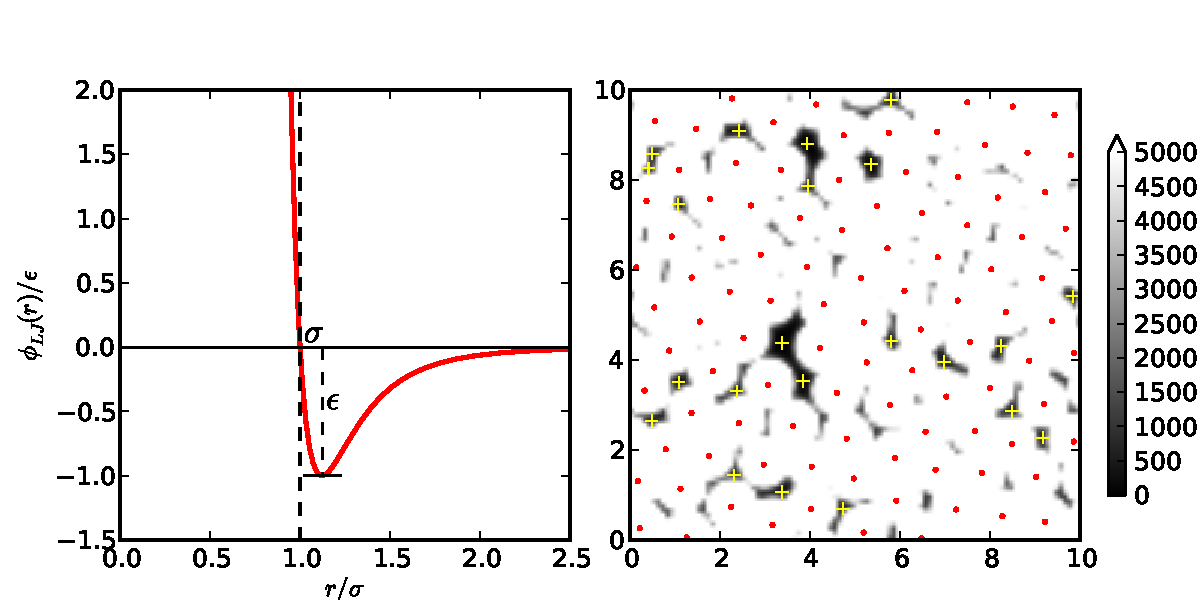
\includegraphics[width=\textwidth]{plots/lj}
  \caption{Links: das Lennard-Jones-Potential mit dem typischen Radius
    $\sigma$ und der Tiefe des attraktiven Tals von
    $\epsilon$. Rechts: Energielandschaft für ein LJ-Teilchen in einer
    zweidimensionalen LJ-Flüssigkeit. Rote Punkte markieren die
    Positionen anderer Teilchen, die Graustufen repräsentieren das
    Potential. Die gelben Kreuze markieren lokale Minima. Um diese zu
    finden, wurde zunächst das Potential an $100\times 100$ Punkten
    ausgewertet, und von allen Punkten mit einem Potential kleiner als
    1000 aus eine lokale Minimierung gestartet.}
  \label{fig:ljminima}
\end{figure}

Die Ausgleichsrechnung, also $\min \norm{Ax-b}_2$, und die linearen
Programme sind zwei Spezialfälle von Optimierung, bei denen ein
gefundenes Optimum stets auch ein globales Minimum ist. Das hängt
damit zusammen, dass die Zielfunktionen im Allgemeinen nur ein
(Ausgleichsrechnung) oder gar kein lokales Minimum (lineare
Programmierung) haben. Im Gegensatz dazu finden das Newtonverfahren
oder das Verfahren des steilsten Abstiegs stets nur lokale Minima,
also Punkte mit verschwindendem Gradienten, dafür aber bei fast
beliebiger Zielfunktion.

In der Praxis, und besonders in physikalischen Anwendungen, sind die
Zielfunktionen meist stark nichtlinear und besitzen zahlreiche lokale
Minima. Suchen wir etwa Grundzustände eines komplexen Systems, müssen
wir Minima der Energiefunktion finden, die meist so viele lokale
Nebenminima aufweist, dass es auch für einen Computer unmöglich ist,
alle zu untersuchen.

Als Beispiel betrachten wir ein in der statistischen Physik sehr
beliebtes Modell, das Lennard-Jonesium (LJ). Dabei handelt es sich um
Teilchen, die gemäß einem Potential
\begin{equation}
  \phi_{\text{LJ}}(r) = 4\epsilon\left[\left(\frac{\sigma}{r}\right)^{12} -
    \left(\frac{\sigma}{r}\right)^{6}\right]
\end{equation}
wechselwirken (vgl. Abbildung~\ref{fig:ljminima} links). Das Potential
hat ein Minimum der Tiefe $-\epsilon$ bei $\sqrt[6]{2}\sigma$ und wird
unterhalb $\sigma$ rasch sehr groß. $\phi_{\text{LJ}}$ ist ein
einfaches Modell für Edelgasatome mit einem Durchmesser von etwa
$\sigma$, die sich auf längere Abstände dispersiv ($\sim r^{-6}$)
anziehen.

In einer solchen zweidimensionalen Lennard-Jones-Flüssigkeit aus 100
Teilchen in einer $10\sigma\times 10\sigma$-Box wählen wir nun ein
Teilchen aus und halten die Koordinaten aller anderen Teilchen
fest. Abbildung~\ref{fig:ljminima} rechts zeigt die potentielle
Energie in Abhängigkeit von der Position des ausgewählten
Teilchens. Dies ist aber nichts anderes als ein zweidimensionaler
Schnitt durch die potentielle Energie als Funktion \emph{aller}
Teilchenkoordinaten. Um die lokalen Minima zu bestimmen, wurde
zunächst auf einem $100\times 100$-Raster das Potential ausgewertet,
und von allen hinreichend niedrigen Punkten aus eine lokale
Minimierung gestartet. Da bereits dieser Schnitt über 20 lokale Minima
aufweist, kann man sich vorstellen, wie viele lokale Minima die
Energie als Funktion aller 200 Teilchenkoordinaten aufweist.  Wegen
des ``Curse of dimension'' ist es in diesem Fall nicht mehr möglich,
eine Rasterung vorzunehmen. Es ist also aussichtslos, sämtliche lokale
Minima mit Hilfe eines lokalen Minimierungsverfahrens zu suchen.

Im Folgenden lernen wir zwei heuristische Methoden kennen, die auch
unter solchen Bedingungen meist akzeptable Näherungen für das globale
Minimum finden.

\subsection{\keyword{Simulated annealing}}

Simulated Annealing (Simulierte Abkühlung) basiert auf der
Beobachtung, dass durch gesteuerte, langsame Abkühlung das Wachstum
besonders gleichmäßiger Kristalle gefördert wird. Dies macht man sich
zum Beispiel bei der Härtung von Stahl zu Nutze. Letztendlich ist
Kristallisation aber nichts anderes als ein Optimierungsprozess, da
der Einkristall die energetisch minimale Struktur ist.

Um dies auf ein Optimierungsproblem zu übertragen, legt man die
Boltzmann-Statistik der statistischen Physik zugrunde, die besagt,
dass bei Temperatur $T$ alle Zustände gemäß
\begin{equation}
  P_T(x)\sim e^{-\beta E(x)}
\end{equation}
verteilt sind, wobei $E$ die potentielle Energie des Systems im
Zustand $x$ ist und $1/\beta=k_BT$ mit der Boltzmannkonstanten $k_B$.

Sei nun $x_0$ das globale Minimum der Energiefunktion $E$. Dann ist
für alle $x$
\begin{equation}
  P_T(x)\sim e^{-\beta E(x)} = e^{-\beta E(x_o)}e^{\beta [E(x_0) - E(x)]}
  \sim e^{-\beta [E(x) - E(x_0)]} \le 1,
\end{equation}
da $E(x) - E(x_0)\ge 0$. Bei niedrigen Temperaturen ist $\beta$ sehr
groß, so dass alle Zustände mit einer größeren Energie als $E(x_0)$
rasch sehr unwahrscheinlich werden. Durch Abkühlen wird es also
tatsächlich sehr wahrscheinlich, das globale Minimum zu finden. Um
damit ein Optimierungsproblem $\min_{x} E(x)$ global zu lösen, fassen
wir die Elemente der zulässigen Menge als Zustände auf, und die zu
minimierende Funktion $E$ als Energie dieser Zustände.

Im Prinzip könnte man nun mit Hilfe der Verwerfungsmethode versuchen,
$P_T$-verteilte zufällige Zustände zu erzeugen. Wie wir im
Eingangsbeispiel gesehen haben, schwankt die Energielandschaft
allerdings oft stark, so dass die meisten Punkte extrem kleine
Akzeptanzraten hätten. Dies sorgt für astronomisch hohe
Verwerfungsraten, so dass es mit dieser Methode unmöglich ist, die
Boltzmann-Verteilung abzutasten. In der statistischen
Physik benutzt man als Ausweg das \emph{Monte-Carlo-Sampling} von
N. Metropolis.

\index{Monte-Carlo-Sampling}\index{Metropolis-Methode} Ziel dieser
Methode ist es, nacheinander Punkte $x_i$ zu erzeugen, die
$P_T$-verteilt sind, so dass die Folge $x_i$ unsere Verteilung
repräsentiert. Nehmen wir nun an, dass unser aktueller Punkt bereits
$P_T$-verteilt gezogen wurde, müssen wir also den nächsten Punkt so
wählen, dass wir die Verteilung nicht ändern. Dazu wählen wir
zufällige Übergänge $x_i\to x_{i+1}$ so, dass für zwei beliebige
Punkte $x$ und $y$ die Übergänge $x\to y$ und $y\to x$ mit gleicher
Wahrscheinlichkeit ausgewählt werden. Eine Möglichkeit ist der
klassische \emph{Metropolis-Schritt}
\begin{equation}
  y = x_i + d,\quad\text{mit}\; d\;\text{gleichverteilt auf einer
    Kugel vom Radius}\; r.
\end{equation}
$r$ ist dabei in gewisser Weise die maximale Schrittweite dieses
Algorithmus. Dies erzeugt eine Gleichverteilung der Punkte; um die
korrekte Verteilung zu erzeugen, setzen wir $x_{i+1}=y$ mit
Wahrscheinlichkeit proportional zu
\begin{equation}
  p(y) = \min(e^{-\beta [E(y) - E(x_i)]}, 1) = \min(P(y)/P(x_i), 1).
\end{equation}
Ist also $E(y) \le E(x_i)$, akzeptieren wir den Schritt immer, ist
$E(y) > E(x_i)$, dann mit Wahrscheinlichkeit $e^{-\beta [E(y) -
  E(x_i)]}$. Die Verwerfungsmethode liefert uns einen einfachen
Algorithmus, diese Verteilung zu erzeugen --- wir ziehen eine
Standardzufallszahl $u$ und setzen $x_{i+1}=y$, falls $u<p(y)$ und
$x_{i+1}=x_i$ sonst.

\begin{figure}
  \centering
  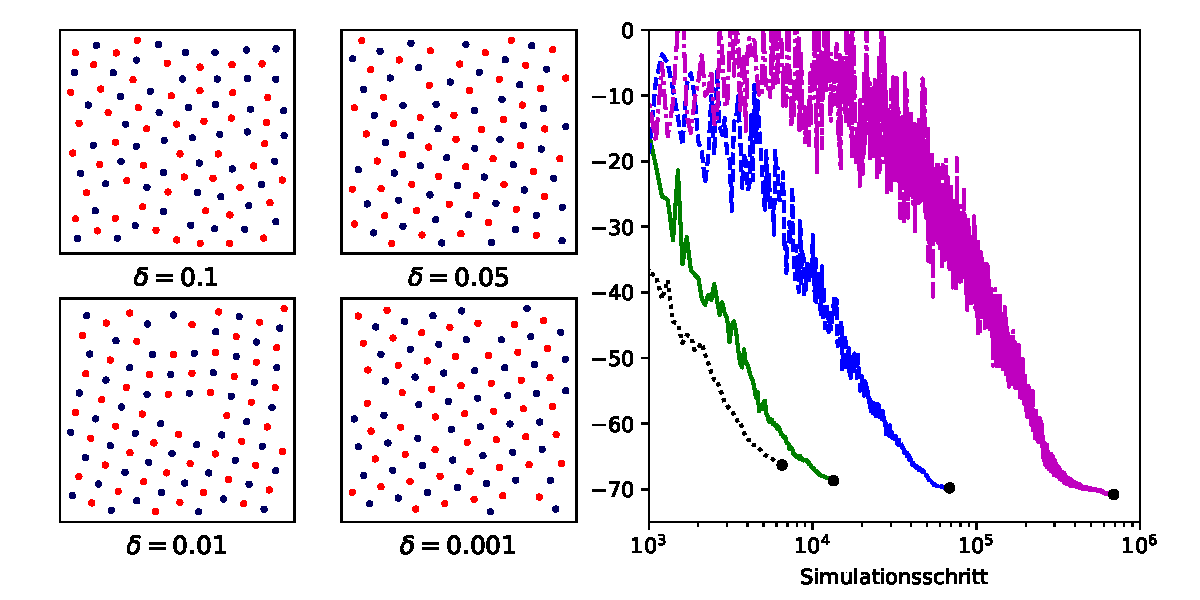
\includegraphics[width=\textwidth]{plots/simulated_annealing}
  \caption{Simulated Annealing eines zweidimensionalen
    Salzschmelzemodells. Links sind die gefundenen Grundzustände für
    verschiedene Abkühlraten $\epsilon$ gezeigt, rechts die
    dazugehörigen potentiellen Energien als Funktion der Zeit (schwarz
    gepunktet $\epsilon=0,1$, grün durchgezogen $\epsilon=0,05$, blau
    gestrichelt $\epsilon=0,01$ und magentafarbene Strichpunkte
    $\epsilon=0,005$). Der eigentlich Grundzustand wäre ein
    NaCl-artiges Gitter, das aber nicht gefunden wird, auch wenn die
    Simulationen immer größere Gitterflächen zeigen. Die Unterschiede
    in den finalen Energien sind sehr klein, was nochmals zeigt,
    dass auch dieses Problem sehr viele Nebenminima aufweist.}
  \label{fig:simanneal}
\end{figure}

Beim Simulated Annealing werden die Punkte mit Hilfe der
Metropolis-Methode $P_T$-verteilt erzeugt, und gleichzeitig die
Temperatur langsam abgesenkt. Dadurch sollte die Verteilung langsam
gegen $P_0$ konvergieren, in der nur noch das oder die globalen Minima
eine nichtverschwindende Wahrscheinlichkeit haben. Dementsprechend
konvergiert die Folge $x_i$ gegen ein globales Minimum. Problematisch
kann sein, dass die korrekte Verteilung der $x_i$ natürlich nur
sichergestellt werden kann, wenn auch hinreichend viele $x_i$
generiert werden. Das bedeutet, dass die Temperatur langsam abgesenkt
werden sollte, wobei ``langsam'' vom Problem abhängt.

Die funktionale Form der Temperaturkurve ist frei
wählbar. Typischerweise wählt man eine exponentielle Form
\begin{equation}
  T_{i+1} = (1-\delta)T
\end{equation}
mit kleinem $\delta > 0$ (etwa $10^{-6}$). Dann wird natürlich $T=0$
nie erreicht, allerdings sind kleine $T$ meist ausreichend. Alternativ
kann man eine lineare Form wählen
\begin{equation}
  T_{i+1} = T_i - \delta,\quad\text{solange}\; T_i>\delta.
\end{equation}

Simulated Annealing funktioniert nicht nur mit dem
Metropolis-Schritt, sondern auch mit allen anderen möglichen
Monte-Carlo-Schritten, wie sie in der Vorlesung
"`Simulationsmethoden"' behandelt werden. Auch Molekulardynamik kann
genutzt werden, um Zustände im kanonischen Ensemble, also bei
konstanter Temperatur, zu erzeugen.

\subsubsection{Beispiel: zweidimensionale Salzschmelze}
Als Beispiel zeigt Abbildung~\ref{fig:simanneal} Daten zur
Kristallisation eines einfachen NaCl-Modells. Hier wechselwirken die
Teilchen mit einem Potential
\begin{equation}
  \phi_{ij} = q_iq_j\frac{4\sigma\epsilon}{r}  +
  \begin{cases}
    4\epsilon\left(\frac{\sigma}{\norm{x_i-x_j}}^{12} -
      \frac{\sigma}{\norm{x_i-x_j}}^{6}\right) + \epsilon
    & \text{für}\; \norm{x_i-x_j} < \sqrt[6]{2}\sigma\\
    0 & \text{sonst}.
  \end{cases}
\end{equation}
Die Hälfte der Teilchen haben dabei Ladung $q_i=1$, die andere Hälfte
$q_i=-1$. Der erste Teil des Potentials ist das Coulombpotential
aufgrund der elektrostatischen Anziehung bzw. Abstoßung, der zweite
besteht aus dem repulsiven Teil des LJ-Potentials und simuliert die
Volumenausschlußwechselwirkung. Die Teilchen arrangieren sich aufgrund
des Volumenausschlusses recht schnell in einem Gitter, es kostet
allerdings sehr viel Energie, dann Plätze zu tauschen. Daher gibt es
zahlreiche Nebenminima.

Im Beispiel wurde statt des Metropolisalgorithmus eine
Molekulardynamiksimulation mit Hilfe von ESPResSo~\cite{espresso}
benutzt. Auch hier kann die Temperatur gesteuert werden. Links zeigt
Abbildung~\ref{fig:simanneal} die gefundenen Annäherungen für
Grundzustände, rechts sind deren Energien gezeigt. Trotz der recht
langen Simulationszeiten sind die gefundenen Grundzustände noch nicht
optimal --- das wäre ein quadratisches Gitter mit alternierender
Besetzung. Eine Monte-Carlo-Simulation könnte hier übrigens deutlich
effizienter sein, allerdings nur, wenn auch sogenannte
Identitätstauschschritte benutzt werden, bei denen zwei beliebige
Teilchen ihre Ladungen austauschen und so die Energiebarrieren
umgehen.

\subsection{Genetische Algorithmen}

Für die Untersuchung noch komplexerer Kristallstrukturen, etwa mit -3-
und 5-wertigen Ionen, ist der obige Ansatz immer noch nicht effizient
genug, da er dazu neigt, in lokalen Minima stecken zu bleiben. Besser
wäre es, Elementarzellen des Kristalls durchzuprobieren, und nach
derjenigen mit minimaler Energie zu suchen. Leider ist auch diese
Optimierung noch sehr umfangreich, und die Menge der möglichen
Kristallstrukturen lässt sich nicht einfach als Vektorraum beschreiben.

In solchen Fällen sind genetische Algorithmen ein biologisch
inspirierter Ansatz, um trotzdem eine globale Minimierung durchführen
zu können. Dabei ist das \emph{Genom} nicht mehr ein DNS-Molekül,
sondern eine Zeichenkette aus reellen Zahlen, Bits oder ähnlichem, die
jeweils ein Element der ursprünglichen zulässigen Menge codieren (also
zum Beispiel eine mögliche Elementarzelle). Wir erzeugen zu Beginn der
genetischen Algorithmus zufällig eine große Menge von Individuen (etwa
einige 1000), indem wir zufällige entsprechende Zeichenketten
generieren.

Wie bei der natürlichen Evolution sollen sich im Verlauf die
"`fittesten"' Individuen sich vermehren und ungeeignetere aussterben.
Dazu definieren wir eine \emph{Fitnessfunktion}, die die Güte eines
Genoms bzw.\ des dadurch codierten Individuums misst. Im Falle der
Kristallgitteroptimierung wäre dies zum Beispiel die Energie eines
Gitters, dass aus der Elementarzelle entsteht, die vom Genom codiert
wird.

Wie werden nun Individuen vermehrt? Einfach, indem zufällige, kleine
Änderungen am Genom des sich vermehrenden Individuums vorgenommen
werden und dieses neue Genom in den Pool der vorhanden Individuen
aufgenommen wird. Dabei werden fittere Individuen häufiger
vermehrt. Das kann man auf verschiedene Weisen erreichen, zum
Beispiel, indem stets eine kleine Anzahl von Individuen zufällig
ausgewählt wird, und von diesen das fitteste vermehrt.  Dabei gibt es
zwei Typen von Änderungen am Genom: \emph{Mutationen}, also kleine
zufällige Änderungen im Genom, und \emph{Kreuzungen} zweier guter
Individuen. Dabei werden zufällig Abschnitte der beiden ausgewählten
Individuen zu einem neuen Genom kombiniert.

Um die Menge der Genome konstant zu halten, können bei diesem Prozess
auch Genome entfernt werden. Werden etwa die fittesten Individuen
einer zufällig gewählten Gruppe zur Vermehrung herangezogen, kann
gleichzeitig das am wenigste fitte Element dieser Gruppe gelöscht
werden.

L. Filion und M. Dijkstra~\cite{filion09a} haben einen solchen
Algorithmus benutzt, um die möglichen Kristallstrukturen in binären
kolloidalen Kristallen mit verschiedenen Größen und Ladungen
vorherzusagen. Dabei werden die Elementarzellen durch eine feste
Anzahl von Vektoren dargestellt. Hat die Elementarzelle $n$ Elemente,
stellen $n-1$ Vektoren $B_i$ die Relativpositionen der Elemente in der
Zelle dar, und 3 Vektoren $L_i$ legen die Relativpositionen der
räumlichen Kopien der Elementarzelle fest. In den meisten zufällig so
erzeugten Gittern überlappen Teilchen, so dass auch in diesem Fall ein
weiches Lennard-Jones-Potential die Volumenausschlusswechselwirkung
modelliert. Dadurch werden undefinierte Energiewerte vermeiden.

Zur Vermehrung werden zufällig zwei Individuen gewählt, deren Vektoren
$B_i$ zufällig um maximal $\pm 10\%$ gestreckt werden. Dann wird
zufällig $B_1,\ldots,\,B_k$ vom ersten Individuum mit
$B_{k+1},\ldots,\,B_n$ vom zweiten kombiniert, und analog die
$L_i$. Zusätzlich wird sicher gestellt, dass die $L_i$ linear
unabhängig sind, also tatsächlich ein Gitter aufspannen. Um die
Chancen des neuen Genoms zu erhöhen, wird für dieses die Energie lokal
minimiert, indem die Darstellung geeignet verdreht wird. Es ist durchaus
üblich, physikalisches Wissen in genetischen Algorithmen zu benutzen,
um bessere Genome zu erzeugen.

%%% Local Variables: 
%%% mode: latex
%%% TeX-master: "padc.tex"
%%% TeX-PDF-mode: t
%%% End: 

% Dies ist Teil der Vorlesung Physik auf dem Computer, SS 2012,
% Axel Arnold, Universitaet Stuttgart.
% 
% Dieses Werk ist unter einer Creative Commons-Lizenz vom Typ
% Namensnennung-Weitergabe unter gleichen Bedingungen 3.0 Deutschland
% zugänglich. Um eine Kopie dieser Lizenz einzusehen, konsultieren Sie
% http://creativecommons.org/licenses/by-sa/3.0/de/ oder wenden Sie sich
% schriftlich an Creative Commons, 444 Castro Street, Suite 900, Mountain
% View, California, 94041, USA.

\chapter{Differentialgleichungen}
\index{Differentialgleichung}

Fast alle physikalischen Probleme können durch Differentialgleichungen
(DGLs) beschrieben werden. Auch das einleitende Problem des
Fadenpendels ist wurde ja durch die Differentialgleichung
\begin{equation}
  \ddot\alpha = -\frac{g}{l}\sin(\alpha)
\end{equation}
beschrieben. Die analytische Lösung dieser und der meisten
Differentialgleichungen ist schwierig oder unmöglich, und daher sind
numerische Verfahren zum Lösen von DGLs wichtige Hilfsmittel, um
Modelle mit komplexen DGLs untersuchen zu können.

Im folgenden werden wir numerische Löser für verschiedene Klassen von
Differentialgleichungen kennenlernen. Für gewöhnliche
Differentialgleichungen mit skalarer Variable sind das die
Runge-Kutta-Verfahren, sowie das bereits in der Einleitung
besprochene, sehr gebräuchliche Velocity-Verlet-Verfahren.

Schwieriger ist die Lösung partieller Differentialgleichungen, die
mehrdimensionale Variablen und deren Ableitungen enthalten.  Diese
spielen besonders in der Physik eine wichtige Rolle, weil sie bei bei
zeit- und ortsabhängigen Prozessen quasi automatisch auftreten. Hier
lernen wir einige Bespiele kennen und wie diese mit Hilfe finiter
Differenzen oder Fouriertransformationen numerisch gelöst werden
können.

\section{Gewöhnliche Differentialgleichungen}
\index{Differentialgleichung>gewöhnliche}
\index{Differentialgleichung>explizite}

Wir betrachten Differentialgleichungen der Form
\begin{equation}
  \label{eq:explicitode}
  f^{(m)}(t) = F(t, f(t), \dot f(t), \ldots, f^{(m-1)}(t))
\end{equation}
mit $f:\RR\to\RR^n$. Diese heißen gewöhnlich, da sie nur von einer
Variablen, $t$ abhängen. Wie der Name $t$ schon vermuten lässt, wird
diese Variable meist mit der Zeit assoziert. Die spezielle Form
\eqref{eq:explicitode} wird auch \emph{explizite} gewöhnliche
Differentialgleichung $m$-ter Ordnung genannt, da wir voraussetzen,
dass sich die Gleichung global nach $f^{(m)}(t)$ auflösen lässt, und
$m$ Ableitungen involviert sind. \emph{Implizite} Gleichungen der Form
$F(t, f(t), \dot f(t), \ldots, f^{(m-1)}(t),f^{(m)}(t)) = 0$ sind
numerisch sehr viel schwieriger zu lösen, tauchen aber in der Physik
auch seltener auf, und werden daher hier nicht weiter besprochen.

Für die numerische Lösung beschränken wir uns weiter auf gewöhnliche
Differentialgleichungen erster Ordnung, also von der Form
\begin{equation}
  \label{eq:1storderode}
  \dot f(t) = F(t, f(t)),\quad f(0)\;\text{gegeben}.
\end{equation}
Dies ist tatsächlich keine Einschränkung, da sich jede explizite
Differentialgleichung $m$-ter Ordnung in eine höherdimensionale
Gleichung erster Ordnung transformieren lässt:
\begin{equation}
  \frac{d}{dt}\begin{pmatrix}
    f(t)\\
    \dot f(t)\\
    \vdots\\
    f^{(m-1)}(t)
  \end{pmatrix}
  =
  \begin{pmatrix}
    \dot f(t)\\
    \ddot f(t)\\
    \vdots\\
    f^{(m)}(t) = F(t, f(t), \dot f(t), \ldots, f^{(m-1)}(t))
  \end{pmatrix}
\end{equation}

Die Differentialgleichung des einleitenden Beispiels
\begin{equation}
  \ddot \alpha(t) = -\frac{g}{l}\sin(\alpha(t)),
\end{equation}
oder allgemeiner eine Kraftgleichung der Form
\begin{equation}
  \ddot x(t) = F[x(t)]
\end{equation}
wird so zum Beispiel zu
\begin{equation}
  \label{eq:explicitode}
  \frac{d}{dt}\begin{pmatrix}
    x(t)\\
    \dot x(t)
  \end{pmatrix}
  =
  \begin{pmatrix}
    \dot x(t)\\
    F[x(t)]
  \end{pmatrix}.
\end{equation}  
Der Startwert ist dann $(x(0), \dot x(0))$, also Anfangsposition und
-geschwindigkeit.

\subsection{\keyword{Runge-Kutta-Verfahren}}

Wir betrachten nun das allgemeine Problem~\eqref{eq:1storderode}, also
\begin{equation*}
  \dot f(t) = F[t, f(t)],\quad f(0)\;\text{gegeben}.
\end{equation*}
Wir suchen eine diskretisierte Näherung $y_n \approx f(t_n)$ mit
äquidistanten Zeitpunkten $t_n=n h$, $n=0,1,\ldots$, also Schrittweite
$h$. Es gilt
\begin{equation}
  f(t_{n+1}) = f(t_n+h) = f(t_n) + \int_{t_n}^{t_n+h} \dot f(t)\,dt
  =  f(t_n) + \int_{t_n}^{t_n+h} F[t, f(t)]\,dt.
\end{equation}
Da $y_0 = f(0)$ gegeben ist, liegt es nahe, $y_1 \approx f(h)$ durch
numerische Integration zu bestimmen, dann $y_2 \approx f(2h)$ durch
numerische Integration aus $y_1$ und so weiter. Das Problem dabei ist,
dass der Integrand $F[t, f(t)]$ die zu findende Funktion $f$
enthält. Um also $f(t)$ an Stellen $t\in [t_n, t_n + h]$ annähern zu
können, müssen wir die Zwischenwerte von $f$ wiederum durch
Integration gewinnen. Dies führt zur allgemeinen Form eines
$s$-stufigen Runge-Kutta-Verfahrens
\begin{equation}
  y_{n+1} = y_n + h\sum_{j=1}^s b_j k_j
\end{equation}
mit
\begin{equation}
  \label{eq:rkkj}
  k_j = F(t + h c_j, y_n + h \sum_{k=1}^s a_{jk} k_k)
\end{equation}
und Verfahrenskonstanten $b,c\in\RR^s$ und
$A=(a_{jk})\in\RR^{s,s}$. Die $k_j$ sind also Näherungen für $F[t + h
c_j, f(t_n + h c_j)]$ und erscheinen auf beiden Seiten
von~\eqref{eq:rkkj}. Ist $F(t,y)$ eine nichtlineare Funktion, ist eine
solche implizite Gleichung nur aufwändig zu lösen.

\index{Runge-Kutta-Verfahren>explizite}%
Daher werden meist \emph{explizite} Runge-Kutta-Verfahren verwendet,
bei denen $A$ eine linke untere Dreiecksmatrix mit Nulldiagonale ist,
also $a_{jk} = 0$ für $k\ge j$. Dann werden zur Berechnung von $k_j$
nur $k_k$, $k=1(1)j-1$ benötigt, die bereits berechnet sind. Eine
Implementierung eines Runge-Kutta-Verfahrens ähnelt dann sehr dem
Gauß-Seidel-Verfahren, dass ebenfalls die Zeilen der zu lösenden
Matrix sequentiell abarbeitet.

Das man trotzdem auch implizite Verfahren, also mit allgemeiner
Matrix, in Betracht zieht, hängt damit zusammen, dass diese stabiler
sind, und auch sogenannte steife DGLs lösen können. Ist $A$ linke
untere Dreiecksmatrix, aber die Diagonale nicht Null, spricht man von
DIRKs, diagonal-impliziten Runge-Kutta-Verfahren. Diese lassen sich
noch mit verhältnismäßig begrenztem Aufwand lösen, da pro $k_j$
lediglich eine eindimensionale Gleichung gelöst werden muss.

Der Fehler von Runge-Kutta-Verfahren wird üblicherweise durch die
Konvergenz- und Konsistenzordnung beschrieben. Die Konvergenzordnung
$p$ besagt, dass $\max \norm{y_n - f(t_n)} = \O(h^p)$, d.h.\ die
Näherung konvergiert gleichmäßig gegen $f(t_n)$. Die Konvergenz ist
meist schwer zu beweisen, einfacher ist die Konsistenzordnung $p$, die
nur fordert, dass $\norm{y_{n+1} - f(t_{n+1})} = \O(h^p)$, falls
$y_n=f(t_n)$. Konsistenz besagt also lediglich, dass ein Schritt
prinzipiell konvergiert. Ist die Funktion $F$ Lipschitz-stetig, also
etwa genügend glatt, dann gilt allerdings Konsistenzordnung =
Konvergenzordnung.

\index{Butcher-Tableau}%
Im folgenden werden einige der gebräuchlicheren Runge-Kutta-Verfahren
angegeben. Dabei hat sich das \emph{Butcher-Tableau}
\begin{center}
  \renewcommand{\arraystretch}{1.3}
  \begin{tabular}{r|l}
    c & A \\\hline
    & $b^T$
  \end{tabular}
\end{center}
als kurze Darstellung etabliert. Die $j$-te Zeile gibt an, zu welchen
Zeitpunkt $t_n + hc_j$ die Näherung $k_j$ berechnet wird, $a_{jk}$
sind die zu den benutzten Elementen $k_k$ gehörigen Gewichte der
numerischen Integration, und $b_j$ sind die Gewichte der
Näherungen $k_j$ in der Integration zu $y_{n+1}$.

Die Konstanten ergeben sich aus den benutzten
Quadraturformeln. Allerdings gibt es neben der Bedingung, dass die
Formeln möglichst explizit sein sollten, noch weitere
Stabilitätsbedingungen, die hier aber nicht beschrieben werden
können. Daher kann man nicht einfach beliebige Quadraturformeln
kombinieren, sondern sollte bei den im folgenden beschriebenen,
gebräuchlichen Formeln bleiben.

\subsubsection{Explizites Eulerverfahren}
\index{Eulerverfahren>explizites}

\begin{center}
  \renewcommand{\arraystretch}{1.3}
  \begin{tabular}{r|l}
    0 & \\\hline
    & 1
  \end{tabular}
\end{center}

Das Butcher-Tableau besagt nichts anders, als dass
\begin{equation}
  y_{n+1} = y_n + h F(t_n, y_n) \approx f(t_n) + h f'(t_n).
\end{equation}
Es handelt sich als um die direkte Integration per Rechteckregel, und
damit um ein Verfahren der Ordnung 1, d.h.\ der globale Fehler
$\O(h)$. Diese Verfahren entspricht der einfachen
Integration~\eqref{eq:simple} im einleitenden Beispiel. Das explizite
Eulerverfahren ist nicht sehr genau und nur für global
Lipschitz-stetige $F$ stabil. Daher sollte man es bei praktischen
Anwendungen im allgemeinen vermeiden.

\subsubsection{Implizites Eulerverfahren}
\index{Eulerverfahren>implizites}

\begin{center}
  \renewcommand{\arraystretch}{1.3}
  \begin{tabular}{r|l}
    1 & 1\\\hline
    & 1
  \end{tabular}
\end{center}

Wie der Name schon sagt, ist dies ein implizites Verfahren, genauer,
ein DIRK, bei dem in jedem Schritt die Gleichung
\begin{equation}
  k_1 = F(t_{n+1}, y_n + h k_1)
\end{equation}
gelöst werden muss. Dann ist die neue Näherung $y_{n+1} = y_n + h
k_1$. Durch Einsetzen ergibt sich 
\begin{equation}
  y_{n+1} = y_n + h F(t_{n+1}, y_{n+1}),
\end{equation}
das implizite Eulerverfahren ist also ebenfalls eine Rechteckregel,
aber mit dem neu zu bestimmenden Punkt $y_{n+1}$ als Aufpunkt. Die
Ordnung dieses Verfahrens ist ebenfalls 1. Anders als das explizite
Eulerverfahren ist das implizite Eulerverfahren ziemlich stabil, auch
wenn $F$ nicht Lipschitz-stetig ist. Der Nachteil ist, dass in jedem
Schritt eine nichtlineare Gleichung gelöst werden muss, was das
Verfahren recht aufwändig macht.

\subsubsection{Das Runge-Kutta-Verfahren}
\index{Runge-Kutta-Verfahren>4. Ordnung}

\begin{center}
  \renewcommand{\arraystretch}{1.3}
  \begin{tabular}{r|llll}
    0 & \\
    $\nicefrac{1}{2}$ & $\nicefrac{1}{2}$ \\
    $\nicefrac{1}{2}$ & 0 & $\nicefrac{1}{2}$ \\
    1 & 0 & 0 & 1 \\
    \hline
    & $\nicefrac{1}{6}$ &  $\nicefrac{1}{3}$ & 
    $\nicefrac{1}{3}$ &  $\nicefrac{1}{6}$
  \end{tabular}
\end{center}

Dies ist das erste Runge-Kutta-Verfahren, das zuerst 1901 von Kutta
beschrieben wurde. Wird von dem Runge-Kutta-Verfahren gesprochen, ist
daher dieses Verfahren gemeint. Bei genügend glattem $f$ hat es
Konvergenzordnung 4, ist also deutlich besser als die Eulerverfahren.

Wie können wir das Tableau verstehen?  Wir setzen
$\tau=\nicefrac{h}{2}$. Die zweite und dritte Zeile bestimmen zwei
Näherungen für $F[t_n+\tau, f(t_n+\tau)]$, zunächst mit Hilfe der
linken ($k_2$), und dann der rechten Ableitung ($k_3$). $k_4$ ist dann
eine Näherung für $F[t_n+h, f(t_n+h)]$. Diese Näherungen werden in die
Simpsonregel eingebracht, wobei $k_2$ und $k_3$ mit gleichen Gewichten
eingehen.

%Lotka-Volterra?


% \subsection{Velocity-Verlet-Integration}

% In der Einleitung hatten wir bereits besprochen, wie diese Gleichung
% mit Hilfe des Velocity-Verlet-Verfahrens numerisch gelöst werden kann.
% Dazu hatten wir die Lösung $f(t)$ äquidistant diskretisiert, also an
% Zeitpunkten $t_n=n\delta t$, $n=0,1,\ldots$, betrachtet.

% Wir setzen $\tau=\delta t/2$ und betrachten dann die
% Taylorentwicklungen für $t$ und $t+\delta t= t + 2\tau$ um $t + \tau$:
% \begin{align*}
%   f(t+\delta t) =& f(t+\tau) + \tau
%   \dot f(t + \tau) + \frac{\tau^2}{2}F[f(t+\tau)]
%   + \frac{\tau^3}{6}
%   \frac{d^3}{dt^3} f(t+\tau) + \O(\delta t^4)
%   \intertext{und}
%   f(t) =& f(t+\tau) - \tau
%   \dot f(t + \tau) + \frac{\tau^2}{2}F[f(t+\tau)]
%   - \frac{\tau^3}{6}
%   \frac{d^3}{dt^3} f(t+\tau) + \O(\delta t^4).
% \end{align*}
% und durch Subtraktion
% \begin{equation}
%   f(t+\delta t) = f(t) + 2\tau\,\dot f(t+\tau) + \frac{\tau^3}{3}
%   \frac{d^3}{dt^3} f(t+\tau)+ \O(\tau^4).
% \end{equation}
% Die Geschwindigkeiten an den halben Zeitschritten erhält man einfach
% durch $\dot f(t + \delta t /2) = \dot f(t) + \delta t\, F(t, f(t)) /
% 2$.

% Zusammengefasst ergibt sich der folgende \emph{Velocity-Verlet-Algorithmus}:
% \begin{align}
%   v\left(t + \frac{\delta t}{2}\right) &= v(t) + \frac{\delta t}{2} F(t) \\
%   f(t + \delta t) &= f(t) + v\left(t + \frac{\delta t}{2}\right) \\
%   v(t + \delta t) &= v\left(t + \frac{\delta t}{2}\right) + \frac{\delta t}{2}
%   F(t + \delta t),
% \end{align}
% der anders als die direkte Vorgehensweise vorher numerisch stabil ist
% und quasi keine Energieschwankungen aufzeigt, vergleiche
% Graph~\ref{fig:energie}. 
% Im Quellcode~\ref{lst:pendel} ist alternativ auch dieser Integrator
% implementiert. Obwohl er nur unwesentlich komplizierter ist als der
% einfache Integrator zuvor, erreicht etwa dieselbe Genauigkeit wie
% dieser mit einem Zehntel der Zeitschritte.

% Ist symplektisch

%3-Körperproblem?


% \section{Partielle Differentialgleichungen}


% \section{Lineare Differentialgleichungen}
% \index{Differentialgleichung>lineare}

% Wir betrachten Differentialgleichungen der Form
% \begin{equation}
%   \sum_{i=0}^n c_n(x)f^{(n)}(x) = d(x).
% \end{equation}
% Beispiele, die wir bereits kennengelernt haben, sind der harmonische
% Oszillator~\ref{eq:harmosz}, die Besselsche
% Differentialgleichung~\eqref{eq:besselode} und die
% Laplace-Gleichung~\eqref{eq:laplace}. Sind die Funktionen $c_n(x)$
% sogar konstant, lassen sich die Lösungen analytisch finden, ansonsten
% bieten sich finite Differenzen oder der Übergang in den Fourierraum
% an.

% Als Beispielproblem betrachten wir wieder die Laplace-Gleichung in
% zwei Dimensionen. 
% \subsection{Lösung durch Diskretisierung}

% Bsp: 2d-Laplace

% \subsection{Lösung im Fourierraum}
% Bsp: 2d-Laplace

% FEM FVM erwähnen
% Wärmeleitung, Diffusion
% Advektionsgleichung?


%%% Local Variables: 
%%% mode: latex
%%% TeX-master: "padc.tex"
%%% TeX-PDF-mode: t
%%% End: 


\raggedright
\printbibliography

\printindex

\end{document}

%%% Local Variables: 
%%% mode: latex
%%% TeX-master: t
%%% TeX-PDF-mode: t
%%% End: 
